\documentclass[11pt]{article}
\usepackage[margin=1in]{geometry}
\usepackage{amsmath, amssymb, amsthm}
\usepackage{mathtools}
\usepackage{hyperref}
\usepackage{algorithm}
\usepackage{algpseudocode}
\usepackage{graphicx}
\usepackage{float}
\usepackage[numbers,sort&compress]{natbib}

\usepackage{color-edits}
\addauthor{ev}{red}

\newtheorem{proposition}{Proposition}
\newtheorem{definition}{Definition}

\title{What Algorithms Can Transformers Learn In-Context?\\ Online selection of online algorithms}
\author{Senem I\c{s}\i{}k}

\begin{document}
\maketitle

\tableofcontents
\bigskip

\section{Introduction}
\label{sec:intro}

In-context learning is the phenomenon by which a sequence model, at test time, executes a procedure inferred from the data it sees in context --- potentially only noisy input-output pairs --- without any weight updates. Prior work has demonstrated transformers' ability to learn simple function classes, such as linear and Boolean functions, in context. The analogous question for online algorithms, however, has received less attention. This is a natural direction: online algorithms make decisions based on the sequence observed so far, while transformers are causal sequence models whose predictions are computed from the preceding context. Can transformers learn this kind of instance adaptability --- recovering and running the right algorithmic strategy for each evolving sequence --- or do they collapse onto a single fixed procedure tuned to the average training distribution?

\subsection{Related Work}

A growing literature studies in-context learning for familiar \emph{learning} rules, including least squares, ridge regression, Lasso, generalized linear models, and gradient descent \cite{akyurek_what_2023,baiTransformersStatisticiansProvable2023,garg_what_2022}. In particular, learning to do linear regression --- that is, learning to learn real-valued linear functions in context --- has attracted substantial attention, and recent work has begun to characterize, either mechanistically or by explicit construction, \emph{how} transformers are able to perform such computations \cite{akyurek_what_2023,baiTransformersStatisticiansProvable2023}. Recent work has also studied the in-context learning ability of transformers and LLMs through the problem of learning to learn certain Boolean function families \cite{bhattamishraUnderstandingInContextLearning2023}. See \cite{dongSurveyIncontextLearning2024} for a survey of the capabilities and challenges of in-context learning. This line of work gives an appealing meta-learning perspective: each prompt instantiates a learning task, and the model is trained to implement a learning rule in its forward pass.
Much less is known, however, about whether transformers can learn to learn and execute \emph{classical online algorithms} specifically. The behavior of such algorithms can in principle be represented as Boolean functions, given a sufficiently rich encoding of the input history, but prior work on Boolean function families \cite{bhattamishraUnderstandingInContextLearning2023} has not considered such online algorithms themselves as the target in-context learning task.

\subsection{Problem Statement}

Motivated by this connection, we introduce a model of in-context learning tailored to online algorithms, using a Bayesian stopping problem with a Normal--Normal conjugate prior as our testbed. We call this setting \emph{online selection of online algorithms}: at test time, the transformer sees a sequence with unknown noise level and must, on the fly, recover from the prefix it has observed the threshold rule corresponding to that noise level.

By varying whether the noise level is fixed or random across training distributions, we engineer a setting that discriminates between two hypotheses about the trained model:
\begin{itemize}
\item \textbf{Learning-algorithm hypothesis.} The transformer infers the noise level in context and applies the corresponding threshold rule, adapting per instance and generalizing across noise levels.
\item \textbf{Shortcut hypothesis.} The transformer applies a single training-distribution-tuned policy that ignores the noise level, matching the oracle in distribution but degrading sharply elsewhere.
\end{itemize}

This paper presents empirical evidence on which hypothesis holds under each training distribution, using payoff, threshold-trajectory, and action-agreement diagnostics on in-distribution, OOD, and per-sequence regime-shift test caches. A first pass at mechanistic interpretability --- linear-probing the frozen models' hidden states for the sufficient statistics, $\sigma$-posterior estimates, and continuation values that the algorithmic hypothesis predicts --- is reported in Section~\ref{sec:probe}, with a planned paired-ensemble permutation test for statistical grounding; additional follow-up tools are outlined in Appendix~\ref{sec:future}.

\section{Setup: A Bayesian Optimal Stopping Problem}
\label{sec:setup}

\subsection{Generative model}

For each sample $i \in \{1, \ldots, N\}$, draw a within-sequence noise scale $\sigma_i$ from a prior, draw a latent mean $\mu_i \sim \mathcal{N}(\mu_0, \tau_0^2)$, then draw a sequence
\[
X_1, X_2, \ldots, X_n \mid \mu_i, \sigma_i \;\overset{\text{i.i.d.}}{\sim}\; \mathcal{N}(\mu_i, \sigma_i^2).
\]
We fix $\mu_0 = 0$, $\tau_0 = 10$, horizon $n = 256$ throughout. The agent observes $X_t$ at each $t \in \{1, \ldots, n\}$ and chooses to \emph{stop} (collect $X_t$) or \emph{continue}; at $t = n$ it must stop. Both $\mu_i$ and (in the unknown-$\sigma$ setting) $\sigma_i$ are latent.

\subsection{Five training distributions}

We instantiate five training distributions, three with $\sigma$ fixed (\emph{static-variance}) and two with $\sigma$ random (\emph{random-variance}):
\begin{itemize}
\item $\mathcal{D}_1$: static, $\sigma = 1$ (data-dominant).
\item $\mathcal{D}_2$: static, $\sigma = 10$ (balanced).
\item $\mathcal{D}_3$: static, $\sigma = 100$ (prior-dominant).
\item $\mathcal{D}_{\mathrm{disc}}$: random, $\sigma \sim \mathrm{Uniform}\{1, 10, 100\}$, each with probability $1/3$.
\item $\mathcal{D}_{\mathrm{logu}}$: random, $\log_{10}\sigma \sim \mathrm{Uniform}(0, 2)$, equivalently $p(\sigma) = 1/(2\sigma\ln 10)$ on $[1, 100]$.
\end{itemize}
Both random-variance priors give equal weight to each decade of $\sigma$ --- the discrete prior trivially, the continuous prior by uniform-in-$\log_{10}\sigma$ construction.

\paragraph{Data- vs.\ prior-dominant regimes.} The labels (data-dominant, balanced, prior-dominant) refer to how much the conjugate posterior mean weights the sample mean $\bar X_t$ versus the prior mean $\mu_0$: at $t = 1$ the data weight is $\tau_0^2/(\tau_0^2 + \sigma^2) = 1/(1 + \rho)$ with $\rho := \sigma^2/\tau_0^2$. With $\tau_0 = 10$ this gives data weight $0.99$ at $\sigma = 1$ (data-dominant), $0.50$ at $\sigma = 10$ (balanced), and $0.01$ at $\sigma = 100$ (prior-dominant). Section~\ref{sec:regimes} tabulates the per-regime values; Appendix~\ref{app:adp-static} contains the derivation.

\paragraph{Supervision schemes (continuation-value / action).} Each training distribution is paired with one of two supervision schemes, abbreviated as the suffixes \texttt{\_cv} and \texttt{\_act} on model names:
\begin{itemize}
\item \emph{continuation-value} (\texttt{\_cv}): MSE regression against the Bayes-optimal continuation value $\widehat C_t^\star$ at every $t$ (real-valued target).
\item \emph{action} (\texttt{\_act}): binary cross-entropy against the oracle action $\mathbf{1}[X_t \ge \widehat C_t^\star]$ (binary target).
\end{itemize}
Five distributions $\times$ two supervisions gives ten trained models. Full loss formulas are in Section~\ref{sec:training-objective}.

The static-variance distributions $\mathcal{D}_1, \mathcal{D}_2, \mathcal{D}_3$ play a double role: training distributions for the single-regime models, and test regimes for all evaluation (Section~\ref{sec:regimes}). We name single-regime models by their training data (D1\_cv, D1\_act, etc.) when we need to disambiguate.

\subsection{Test regimes}
\label{sec:regimes}

Evaluation uses seven static-$\sigma$ test regimes spanning four orders of magnitude. Three coincide with the static-variance training distributions $\mathcal{D}_1, \mathcal{D}_2, \mathcal{D}_3$ at $\sigma \in \{1, 10, 100\}$ (in-prior for both random-variance training distributions). Four additional regimes at $\sigma \in \{0.3, 3, 30, 300\}$ are out-of-distribution for every training prior we use --- $\sigma = 3$ and $\sigma = 30$ interpolate between the discrete training values $\{1, 10, 100\}$ (in-prior support of $\mathcal{D}_{\mathrm{logu}}$ but not $\mathcal{D}_{\mathrm{disc}}$); $\sigma = 0.3$ and $\sigma = 300$ extrapolate beyond the support of both random-variance priors. Each regime corresponds to a noise-to-prior-precision ratio $\rho := \sigma^2/\tau_0^2$ with the data weight at $t = 1$ given by $1/(1 + \rho)$:

\begin{center}
\small
\begin{tabular}{l c c c c l}
\hline
test regime & $\sigma$ & $\sigma^2$ & $\rho$ & data weight at $t = 1$ & character \\
\hline
$\mathcal{D}_{\mathrm{ood,0.3}}$ (extrapolation, low) & $0.3$ & $0.09$  & $0.0009$ & $0.999$ & strongly data-dominant \\
$\mathcal{D}_1$ (data-dominant)              & $1$   & $1$     & $0.01$   & $0.99$  & plug-in is asymptotically Bayes \\
$\mathcal{D}_{\mathrm{ood,3}}$ (interpolation)         & $3$   & $9$     & $0.09$   & $0.92$  & between $\mathcal{D}_{\mathrm{disc}}$ training values \\
$\mathcal{D}_2$ (balanced)                   & $10$  & $100$   & $1$      & $0.50$  & no closed-form is asymptotic \\
$\mathcal{D}_{\mathrm{ood,30}}$ (interpolation)        & $30$  & $900$   & $9$      & $0.10$  & between $\mathcal{D}_{\mathrm{disc}}$ training values \\
$\mathcal{D}_3$ (prior-dominant)             & $100$ & $10000$ & $100$    & $0.01$  & prior-only is asymptotically Bayes \\
$\mathcal{D}_{\mathrm{ood,300}}$ (extrapolation, high)  & $300$ & $90000$ & $900$    & $0.0011$ & strongly prior-dominant \\
\hline
\end{tabular}
\end{center}

\paragraph{Datasets.} Training sequences are sampled fresh from the training distribution at each step (no fixed training set); the meaningful budget is gradient steps $\times$ batch size, specified in Section~\ref{sec:training}. Validation and test sets are pre-generated and held fixed at $N_{\mathrm{val}} = N_{\mathrm{test}} = 10^4$ sequences each (validation drawn from the training distribution, used for checkpoint selection only; test drawn per regime, used for all evaluation). Validation and test sets use disjoint random seeds. The OOD test caches use disjoint seeds and apply the same generative model with $\mu_i \sim \mathcal{N}(\mu_0, \tau_0^2)$ throughout.

\subsection{Bayes-optimal Oracle}
\label{sec:oracle}

Each training distribution induces a Bayes-optimal stopping policy that we use as the labeling target during training and as the in-distribution optimal threshold at evaluation. The continuation value $C_t$ has no closed form, so we approximate it by backward dynamic programming on a discretized belief state and store $\widehat C_t$ as a per-stage threshold table. Algorithms, grid sizing, convergence checks, and the marginal-likelihood derivation that the random-variance case relies on are deferred to Appendix~\ref{app:adp}.

\paragraph{Static-variance setting.} When $\sigma$ is fixed and known, only $\mu$ is latent; the Normal--Normal posterior depends on $X_{1:t}$ only through the running sum $S_t$, equivalently the sample mean $\bar X_t = S_t/t$, and is summarized by a one-dimensional belief --- the conjugate posterior mean $\mu_t$. We discretize $\mu_t$ on a per-stage uniform grid scaled to its marginal standard deviation across sequences and run backward induction with Gauss--Hermite quadrature for the predictive expectation (Appendix~\ref{app:adp-static}).

\paragraph{Random-variance setting.} When both $\mu$ and $\sigma$ are latent, the joint sufficient statistic for the posterior $p(\mu, \sigma \mid X_{1:t})$ is the pair $(S_t, Q_t)$ with $S_t := \sum_{s \le t} X_s$ and $Q_t := \sum_{s \le t} X_s^2$. The marginal log-likelihood $\log p(X_{1:t} \mid \sigma)$ has a closed form in $(S_t, Q_t)$ (equation~\eqref{eq:marginal-loglik}, derived in Appendix~\ref{app:adp-random}). We work in transformed coordinates $(\bar X_t, L_t)$ with $L_t := \log \hat\sigma_t^2$, discretize on a 2D grid with bilinear interpolation, and integrate the mixture predictive over $\sigma$ (a 3-point sum for $\mathcal{D}_{\mathrm{disc}}$, a Gauss--Legendre quadrature on $\log\sigma$ for $\mathcal{D}_{\mathrm{logu}}$) before applying Gauss--Hermite for the per-component expectation (Appendix~\ref{app:adp-random}).

\begin{equation}
\label{eq:marginal-loglik}
\log p(X_{1:t} \mid \sigma) = \mathrm{const}(t) - \frac{t}{2}\log\sigma^2 - \frac{1}{2}\log\!\left(1 + \frac{t\tau_0^2}{\sigma^2}\right) - \frac{1}{2}\!\left[\frac{Q_t}{\sigma^2} - \frac{\tau_0^2 S_t^2/\sigma^4}{1 + t\tau_0^2/\sigma^2}\right].
\end{equation}

\subsection{Labeling}
\label{sec:labeling}

For each training distribution we precompute the corresponding ADP threshold table $\{\widehat C_t\}$ once (Appendix~\ref{app:adp-static} for $\mathcal{D}_1, \mathcal{D}_2, \mathcal{D}_3$; Appendix~\ref{app:adp-random} for $\mathcal{D}_{\mathrm{disc}}, \mathcal{D}_{\mathrm{logu}}$). Both tables expose the same query: given the belief state at time $t$, return $\widehat C_t$.

For each sequence $X_{1:n}$ from training distribution $\mathcal{D}$, at each $t \in \{1, \ldots, n-1\}$ we update the belief state and query the table for $\widehat C_t$, then emit
\[
y_t^{\mathrm{cv}} \;:=\; \widehat C_t,
\qquad
y_t^{\mathrm{act}} \;:=\; \mathbf{1}[X_t \ge \widehat C_t].
\]
At $t = n$, $y_n^{\mathrm{act}} = 1$ deterministically and $y_n^{\mathrm{cv}} = 0$.

\paragraph{Hindsight (offline-prophet) labels.} As an alternative to the ADP-oracle labels, we also consider \emph{offline-prophet} labels --- $y_t^{\mathrm{cv}} := \max_{s > t} X_s$ and $y_t^{\mathrm{act}} := \mathbf{1}[X_t \ge \max_{s > t} X_s]$ --- which inspect the realised suffix rather than its expectation under optimal play. They are computed in $O(n)$ per sequence by a single reverse-cummax pass, with no ADP table. We use these labels to retrain the four random-variance models in Appendix~\ref{app:offline-supervision}; on the Gaussian--Gaussian generative model used here they yield within $0.02$ of the oracle-labeler's $R/R^\star$ on every regime --- a property of fast Gaussian tail decay (the prophet's over-waiting margin stays bounded) rather than a general result, but enough to let the labelling step be replaced by a trivial preprocessor at near-zero payoff cost \emph{on this model}.

\section{Portfolio of Baseline Algorithms}
\label{sec:baselines}

We compare the trained models against eight reference policies. The \emph{per-regime oracle} $\pi^\star_{\mathcal{D}_i}$ knows the test-regime $\sigma$ exactly and is Bayes-optimal under $(\mu_0, \tau_0^2, \sigma_i)$; it sets the per-regime optimal threshold $R^\star$. The \emph{known-$\sigma$ plug-in}, \emph{prior-only}, and \emph{myopic} rules also assume $\sigma$ is known and replace $\mu$ by the sample mean $\bar X_t$, the prior mean $\mu_0$, and the conjugate posterior mean $\mu_t$, respectively. The \emph{MAP-$\sigma$ plug-in} (one variant per training prior, $\mathcal{D}_{\mathrm{disc}}$ and $\mathcal{D}_{\mathrm{logu}}$) is the only data-only baseline that uses a prior over $\sigma$: it estimates $\hat\sigma_t^{\mathrm{MAP}}$ from $X_{1:t}$ via the closed-form posterior~\eqref{eq:marginal-loglik} and plugs the estimate into the known-$\sigma$ rule. The \emph{MLE-$\sigma$ plug-in} does the same but uses the Bessel-corrected within-sequence sample standard deviation $s_t = \sqrt{(Q_t - t\bar X_t^2)/(t-1)}$ as the $\sigma$-estimate, so it has no $\sigma$-prior; the ``MLE'' name is conventional (no prior, as opposed to MAP-$\sigma$) rather than literal (full details in Appendix~\ref{app:baselines}). The \emph{secretary} rule is scale-free: skip the first $\lfloor n/e \rfloor$ observations, accept the first subsequent value above their max. Finally, \emph{offline-hindsight} reports $\mathbb{E}[\max_t X_t]$ --- not implementable online, but a strict upper bound on every online policy. Closed-form expressions for all of these (the standardized continuation-value recursion $\eta_t$, plug-in formulas, and the offline-hindsight integral) are in Appendix~\ref{app:baselines}.

\section{Model and Training}
\label{sec:training}

\subsection{Architecture}

GPT-2 decoder backbone with $L = 8$ layers, embedding dimension $d_{\mathrm{emb}} = 128$, $M = 4$ heads, causal attention mask, no dropout. Roughly $1.6$M parameters. The standard GPT-2 language-modeling head is removed; the model is not trained to predict $X_{t+1}$ from $X_{1:t}$. Each scalar $X_t$ is mapped to the embedding by a learnable affine layer $\mathbf{e}_t = W_{\mathrm{in}}\, X_t + \mathbf{b}_{\mathrm{in}}$, followed by learned positional embeddings. The hidden state $\mathbf{h}_t$ at each position feeds either a continuation-value head $\widehat C_t = \mathbf{w}_{\mathrm{cv}}^\top \mathbf{h}_t + b_{\mathrm{cv}}$ or an action head $\hat a_t = \sigma(\mathbf{w}_{\mathrm{act}}^\top \mathbf{h}_t + b_{\mathrm{act}})$, trained against the oracle labels (Section~\ref{sec:labeling}). The causal mask enforces that the output at position $t$ depends only on $X_{1:t}$, matching the online structure of the stopping problem. Inputs $X_t$ enter raw; the continuation-value head produces $\widehat C_t$ in raw oracle units. No input-scale normalization is applied.

\subsection{Training objective}
\label{sec:training-objective}

We train ten models: five training distributions $\{\mathcal{D}_1, \mathcal{D}_2, \mathcal{D}_3, \mathcal{D}_{\mathrm{disc}}, \mathcal{D}_{\mathrm{logu}}\}$ $\times$ two supervisions (continuation-value, action). The model emits one prediction per timestep $t$ via the causal mask. We supervise at every $t \in \{1, \ldots, n-1\}$ (the terminal $t = n$ has no decision, since the agent must accept $X_n$): each timestep contributes its own oracle label and its own gradient signal, giving $n-1 = 255$ training signals per sequence. The per-sequence losses, with sequence-specific $\sigma_i$ used only for continuation-value loss normalization (the model never sees $\sigma_i$), are
\begin{align*}
\ell_{\mathrm{cv}}(\theta;\, X_{1:n},\, \sigma_i)
&\;=\; \frac{1}{(n-1)\,\sigma_i^{2}}\sum_{t=1}^{n-1}\!\Big(\widehat C_t(X_{1:t};\theta) - y_t^{\mathrm{cv}}\Big)^{\!2}, \\
\ell_{\mathrm{act}}(\theta;\, X_{1:n})
&\;=\; -\frac{1}{n-1}\sum_{t=1}^{n-1}\!\Big[\, y_t^{\mathrm{act}}\,\log \hat a_t + (1 - y_t^{\mathrm{act}})\,\log(1 - \hat a_t)\,\Big].
\end{align*}
Each is the within-sequence mean over per-step terms. The mini-batch loss is the further mean over $B = 64$ sequences sampled fresh from the training distribution.

The $1/\sigma_i^2$ factor normalizes the continuation-value loss so high-$\sigma$ and low-$\sigma$ sequences contribute equally: continuation-value errors scale with $\sigma$, and the divisor puts every regime on a common loss scale --- matching the regime-equal weighting of the headline payoff metric $R/R^\star$. Figure~\ref{fig:diagnostic-logu} shows this for $\mathcal{D}_{\mathrm{logu}}$\_cv: absolute continuation-value error scales with $\sigma$ (left panel); the normalized error is uniform across the prior (right panel).

\begin{figure}[H]
\centering
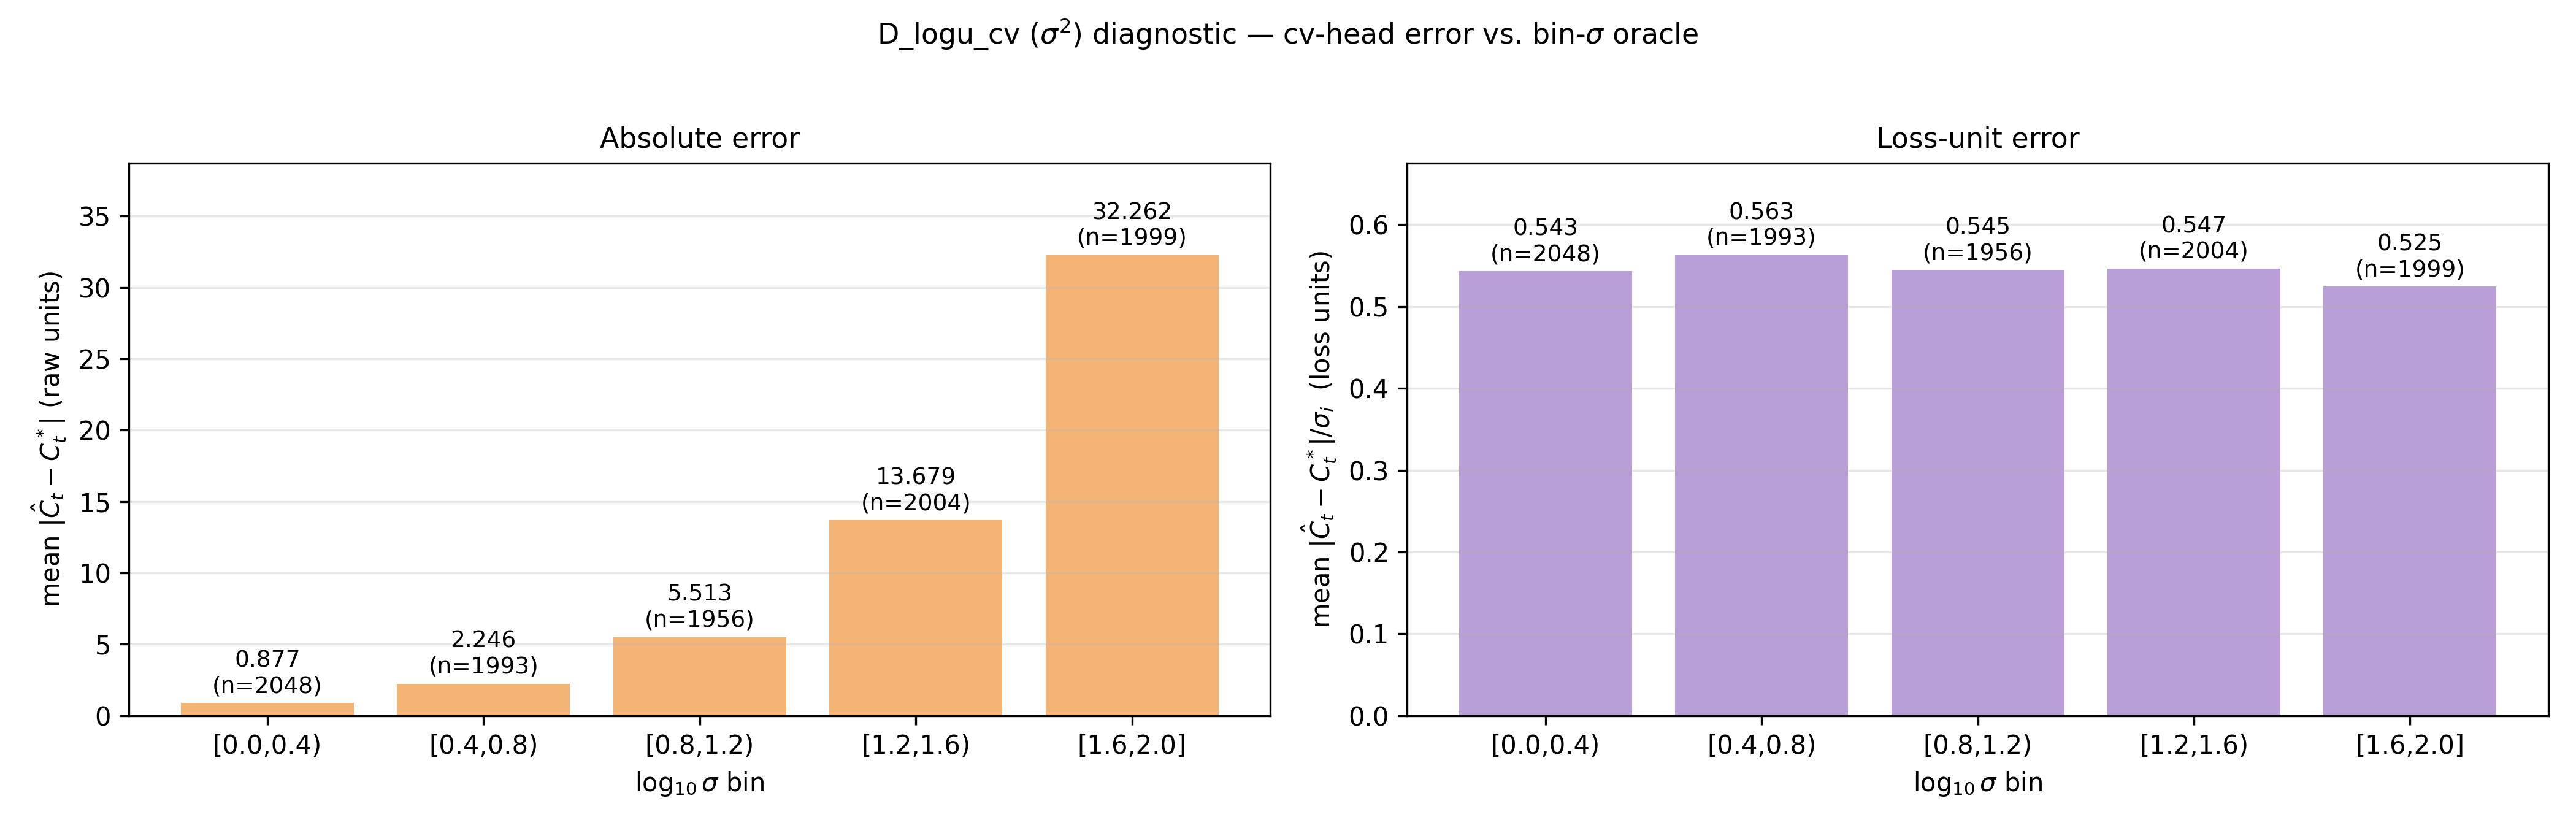
\includegraphics[width=\textwidth]{figures/diagnostic-logu.png}
\caption{Continuation-value error diagnostic for $\mathcal{D}_{\mathrm{logu}}$\_cv. Left: mean $|\widehat C_t - C^\star_t|$ per $\log_{10}\sigma$ bin (raw units); the absolute error scales with $\sigma$. Right: the same error in loss units ($|\widehat C_t - C^\star_t|/\sigma_i$); after the $1/\sigma_i^2$ normalization the error is uniform across all five bins.}
\label{fig:diagnostic-logu}
\end{figure}

Adam, peak learning rate $10^{-4}$, no weight decay, batch size $64$. Static-variance continuation-value models train for $2 \times 10^5$ steps; random-variance continuation-value models for $3 \times 10^5$ (additional steps for in-context regime estimation). Action models train for half their continuation-value counterpart's step count. Cosine schedule with $20\%$ linear warmup; learned absolute position embeddings; checkpoint selection by minimum validation loss.

\section{Experiments and results}
\label{sec:results}

All ten trained models are evaluated on each test regime. We report three metrics per (model, regime) cell: expected payoff $R(\pi; \mathcal{D}_i) := \mathbb{E}[X_{\tau_\pi}]$, competitive ratio $R/R^\star_{\mathcal{D}_i}$ relative to the per-regime oracle (the regime-invariant headline), and per-step action agreement against each baseline. Threshold trajectories (mean $\pm 1$ std over $N_{\mathrm{test}} = 10^4$ test sequences) are reported per continuation-value-supervised model and visualize whether the trained policy adapts to the test regime within the prefix.

\subsection{Static-variance shortcut}
\label{sec:res-static-shortcut}

Each single-regime model matches the per-regime oracle in-distribution and degrades sharply off-diagonally. The three columns labelled $\mathcal{D}_1$\_cv, $\mathcal{D}_2$\_cv, $\mathcal{D}_3$\_cv in the heatmap of Figure~\ref{fig:payoff-and-agreement} (shown in Section~\ref{sec:res-disc}) show this directly: each has a single saturated diagonal cell and pale off-diagonals, with the worst falling to $0.016$ ($\mathcal{D}_3$\_cv on $\mathcal{D}_1$). Action counterparts ($\mathcal{D}_1$\_act, $\mathcal{D}_2$\_act, $\mathcal{D}_3$\_act) are within $0.04$ of the continuation-value entries cell-for-cell.

Figures~\ref{fig:traj-d1cv}--\ref{fig:traj-d3cv} visualize the same effect at the threshold-trajectory level: each model's mean threshold sits flat at its training-distribution scale across all three test regimes, with no adaptation observable in the test prefix.

\begin{figure}[H]
\centering
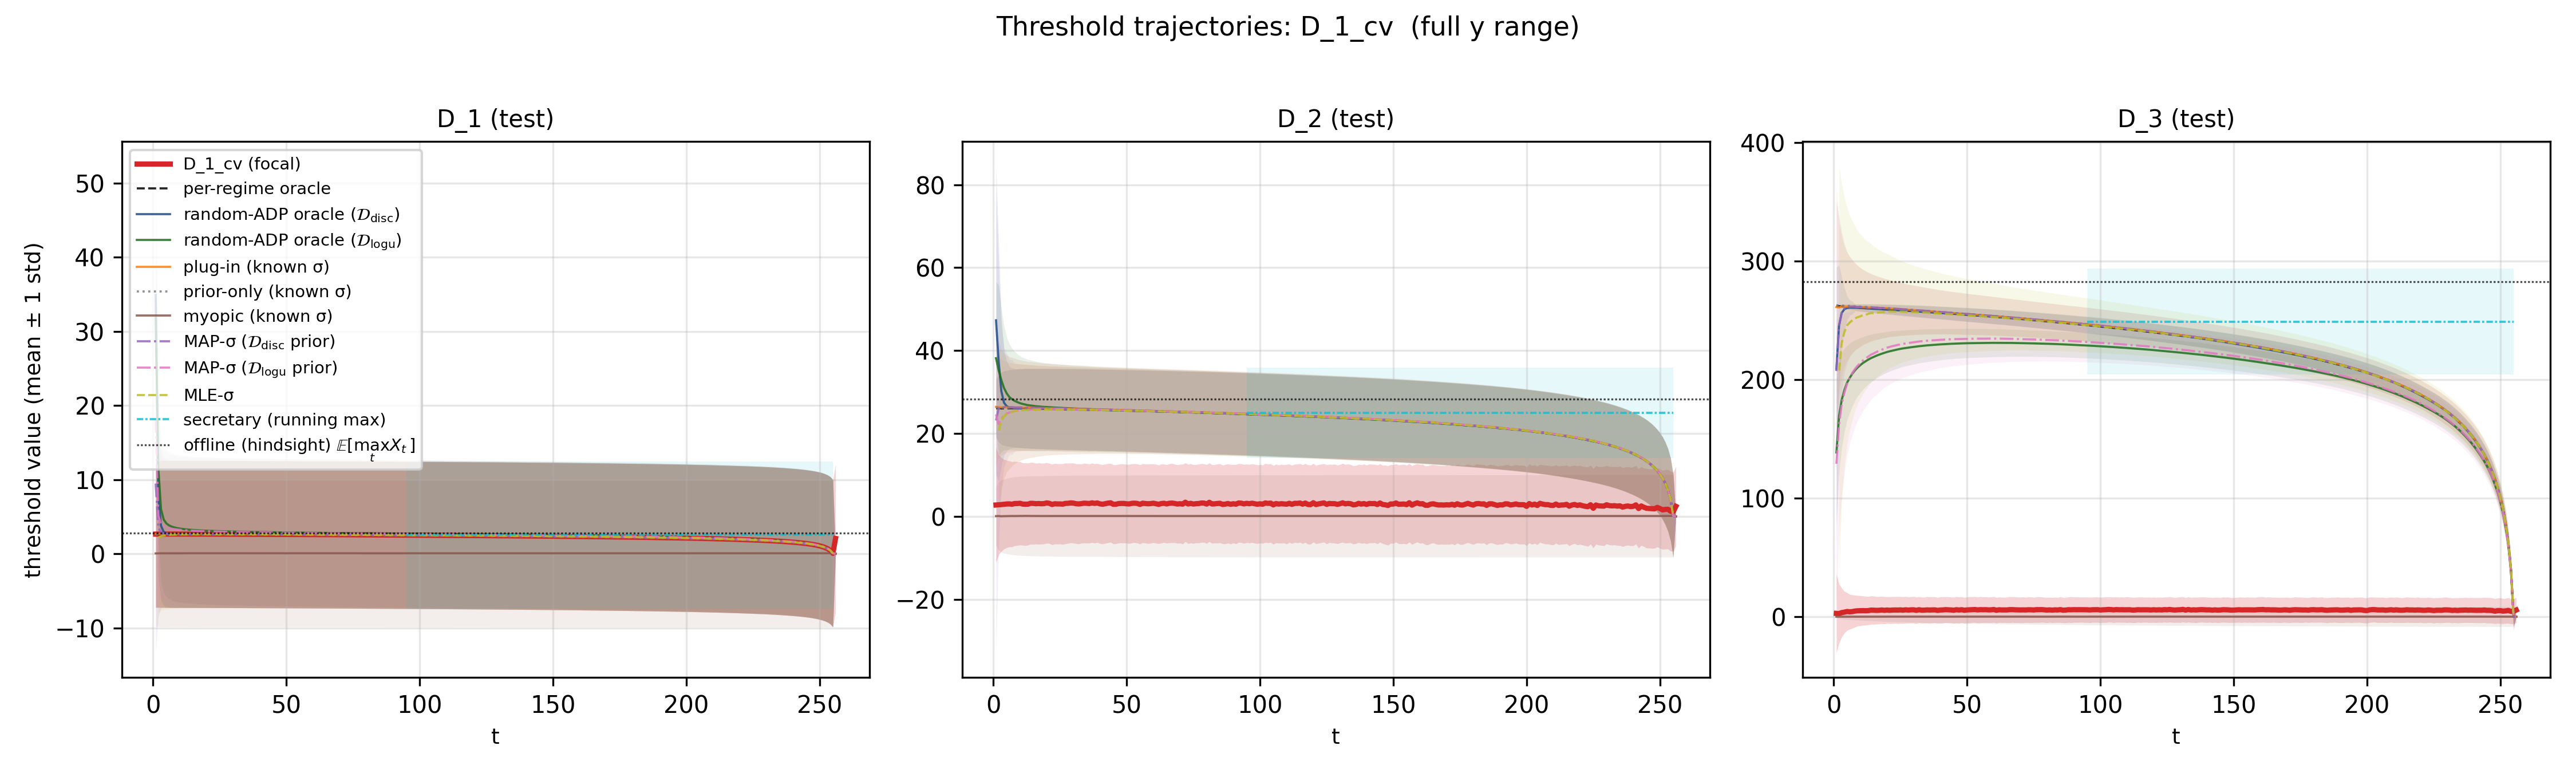
\includegraphics[width=\textwidth]{figures/trajectories-d-1-cv.png}
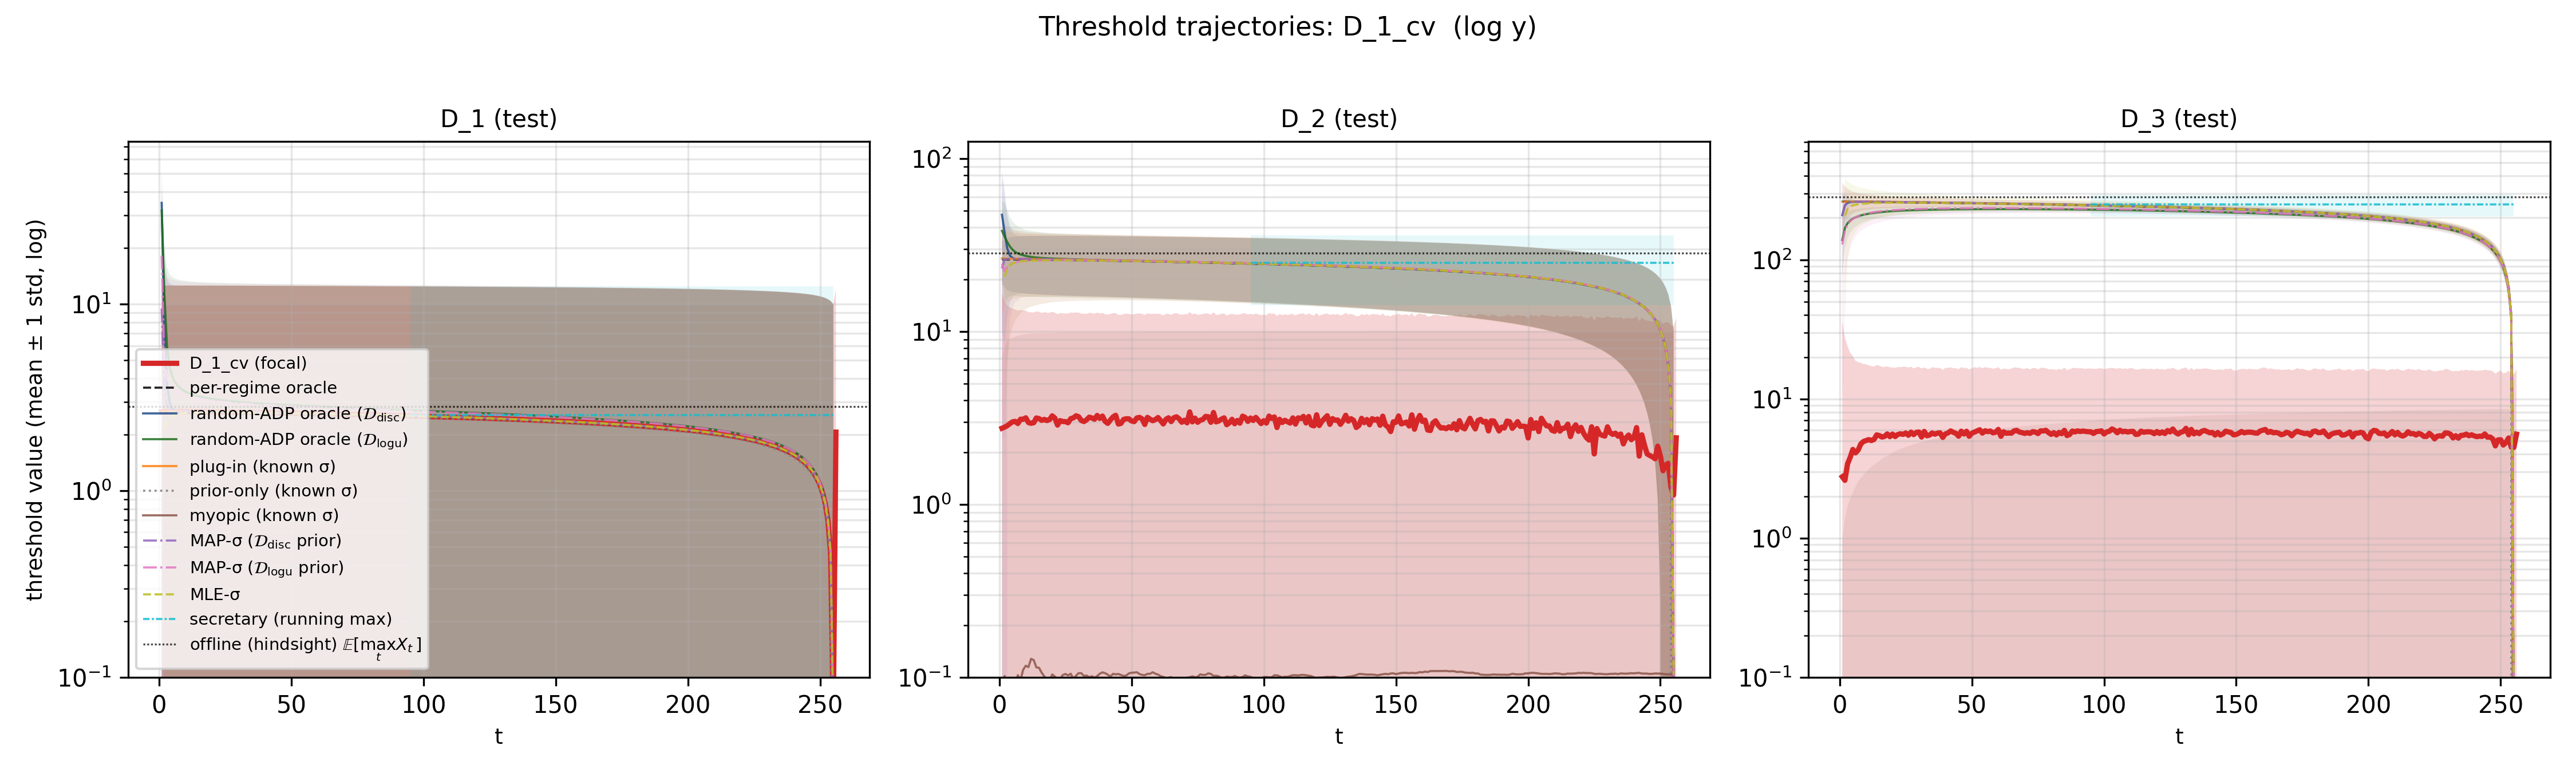
\includegraphics[width=\textwidth]{figures/trajectories-d-1-cv-log.png}
\caption{Threshold trajectories for $\mathcal{D}_1$\_cv (focal model, red, mean $\pm 1$ std band over $N_{\mathrm{test}} = 10^4$ sequences) on each of the three test regimes, with all baselines from Section~\ref{sec:baselines} overlaid. The model's threshold remains at the $\sigma = 1$ scale ($\approx 2.5$) on every regime. Top: linear y, full range (negative-side $\pm 1$ std bands shown). Bottom: log y, negatives clipped at $0.1$.}
\label{fig:traj-d1cv}
\end{figure}

\begin{figure}[H]
\centering
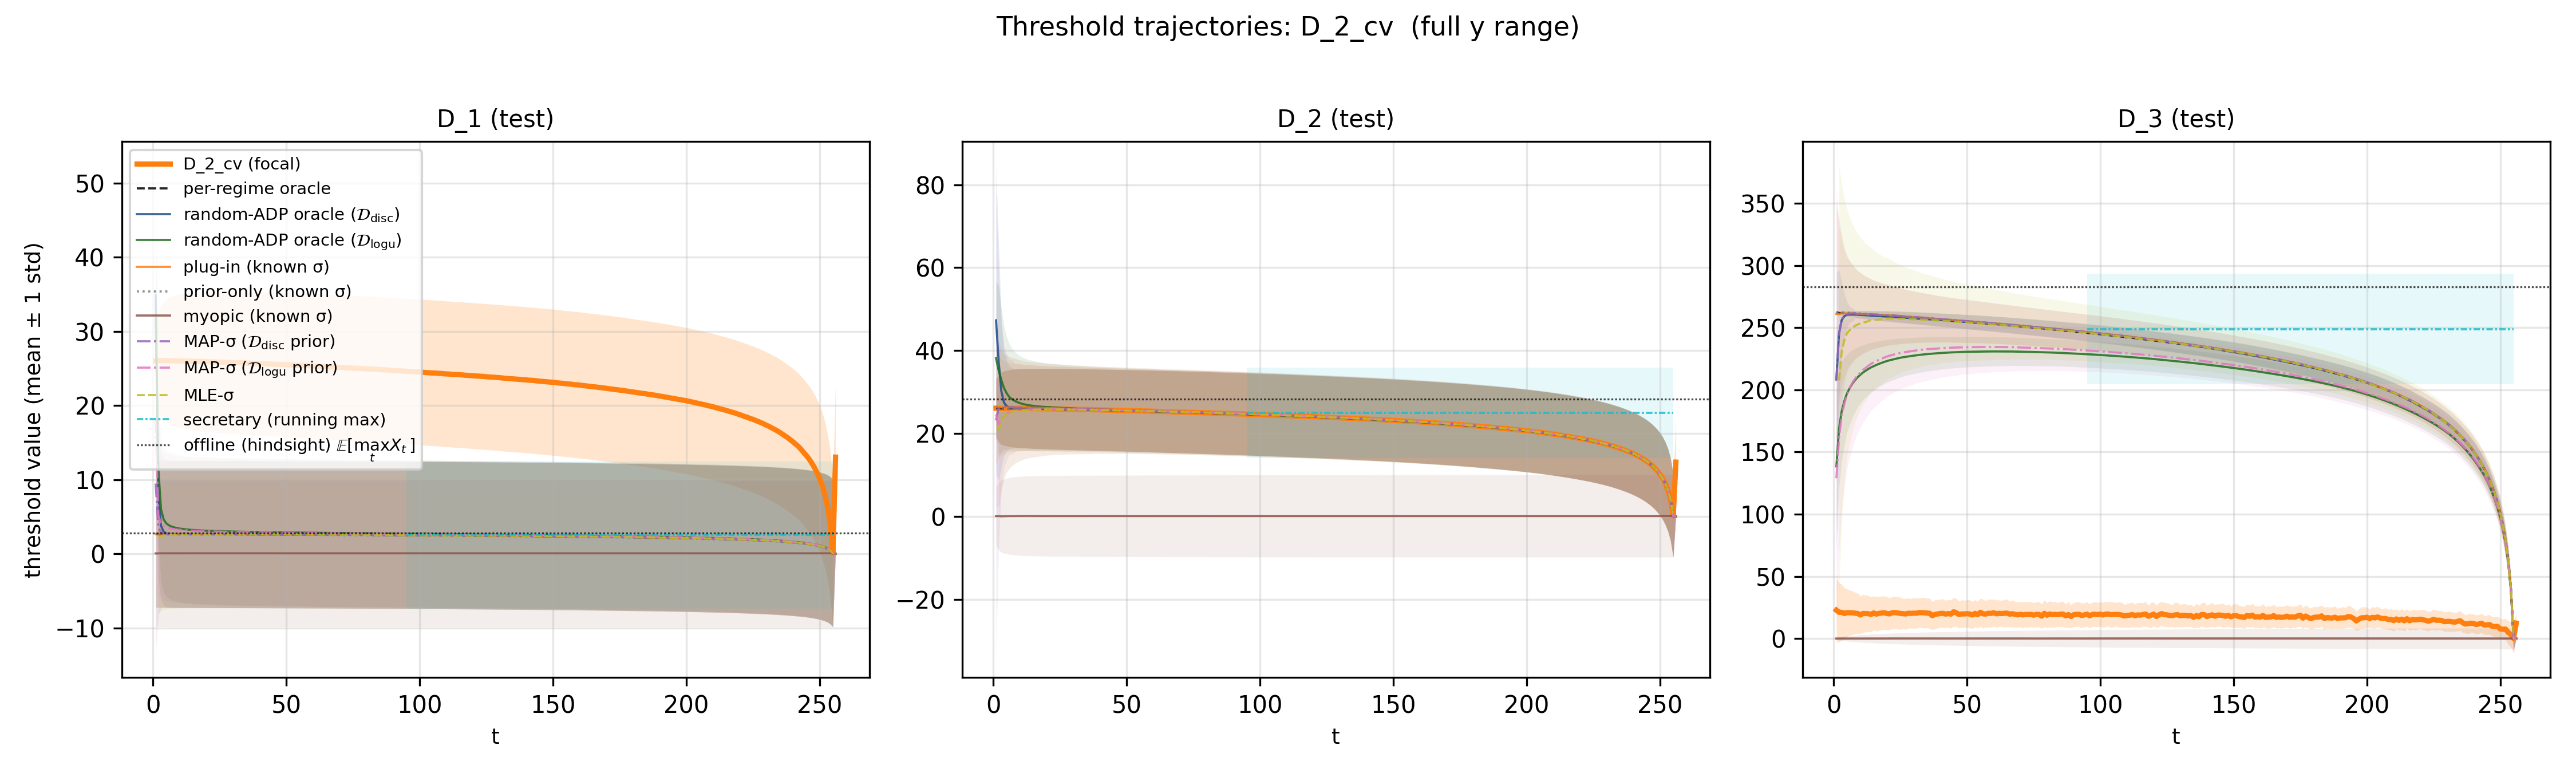
\includegraphics[width=\textwidth]{figures/trajectories-d-2-cv.png}
\caption{Threshold trajectories for $\mathcal{D}_2$\_cv. The model's threshold remains at the $\sigma = 10$ scale ($\approx 26$) on every regime.}
\label{fig:traj-d2cv}
\end{figure}

\begin{figure}[H]
\centering
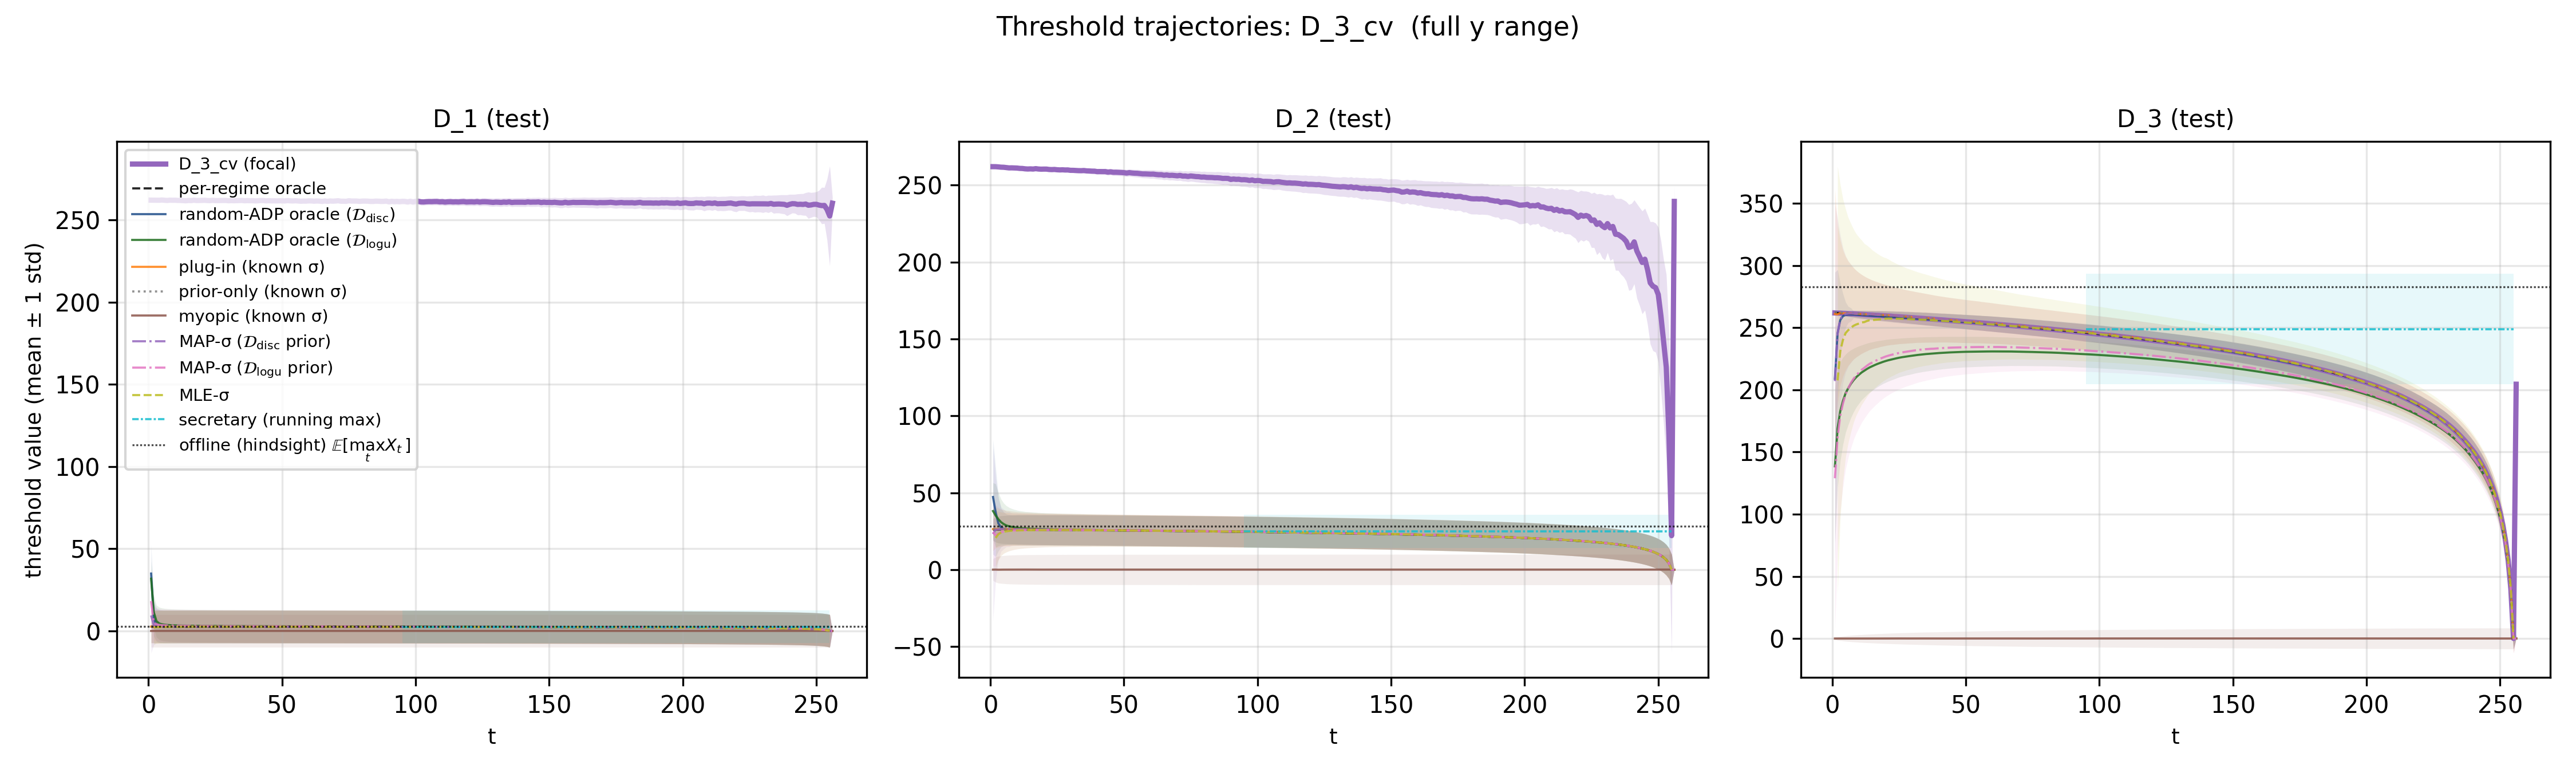
\includegraphics[width=\textwidth]{figures/trajectories-d-3-cv.png}
\caption{Threshold trajectories for $\mathcal{D}_3$\_cv. The model's threshold remains at the $\sigma = 100$ scale ($\approx 260$) on every regime.}
\label{fig:traj-d3cv}
\end{figure}

Figure~\ref{fig:traj-all-cv} overlays all five continuation-value-trained models on each test regime, juxtaposing the three single-regime plateaus against the multi-regime $\mathcal{D}_{\mathrm{disc}}$\_cv adaptation; the contrast is visible at a glance.

\begin{figure}[H]
\centering
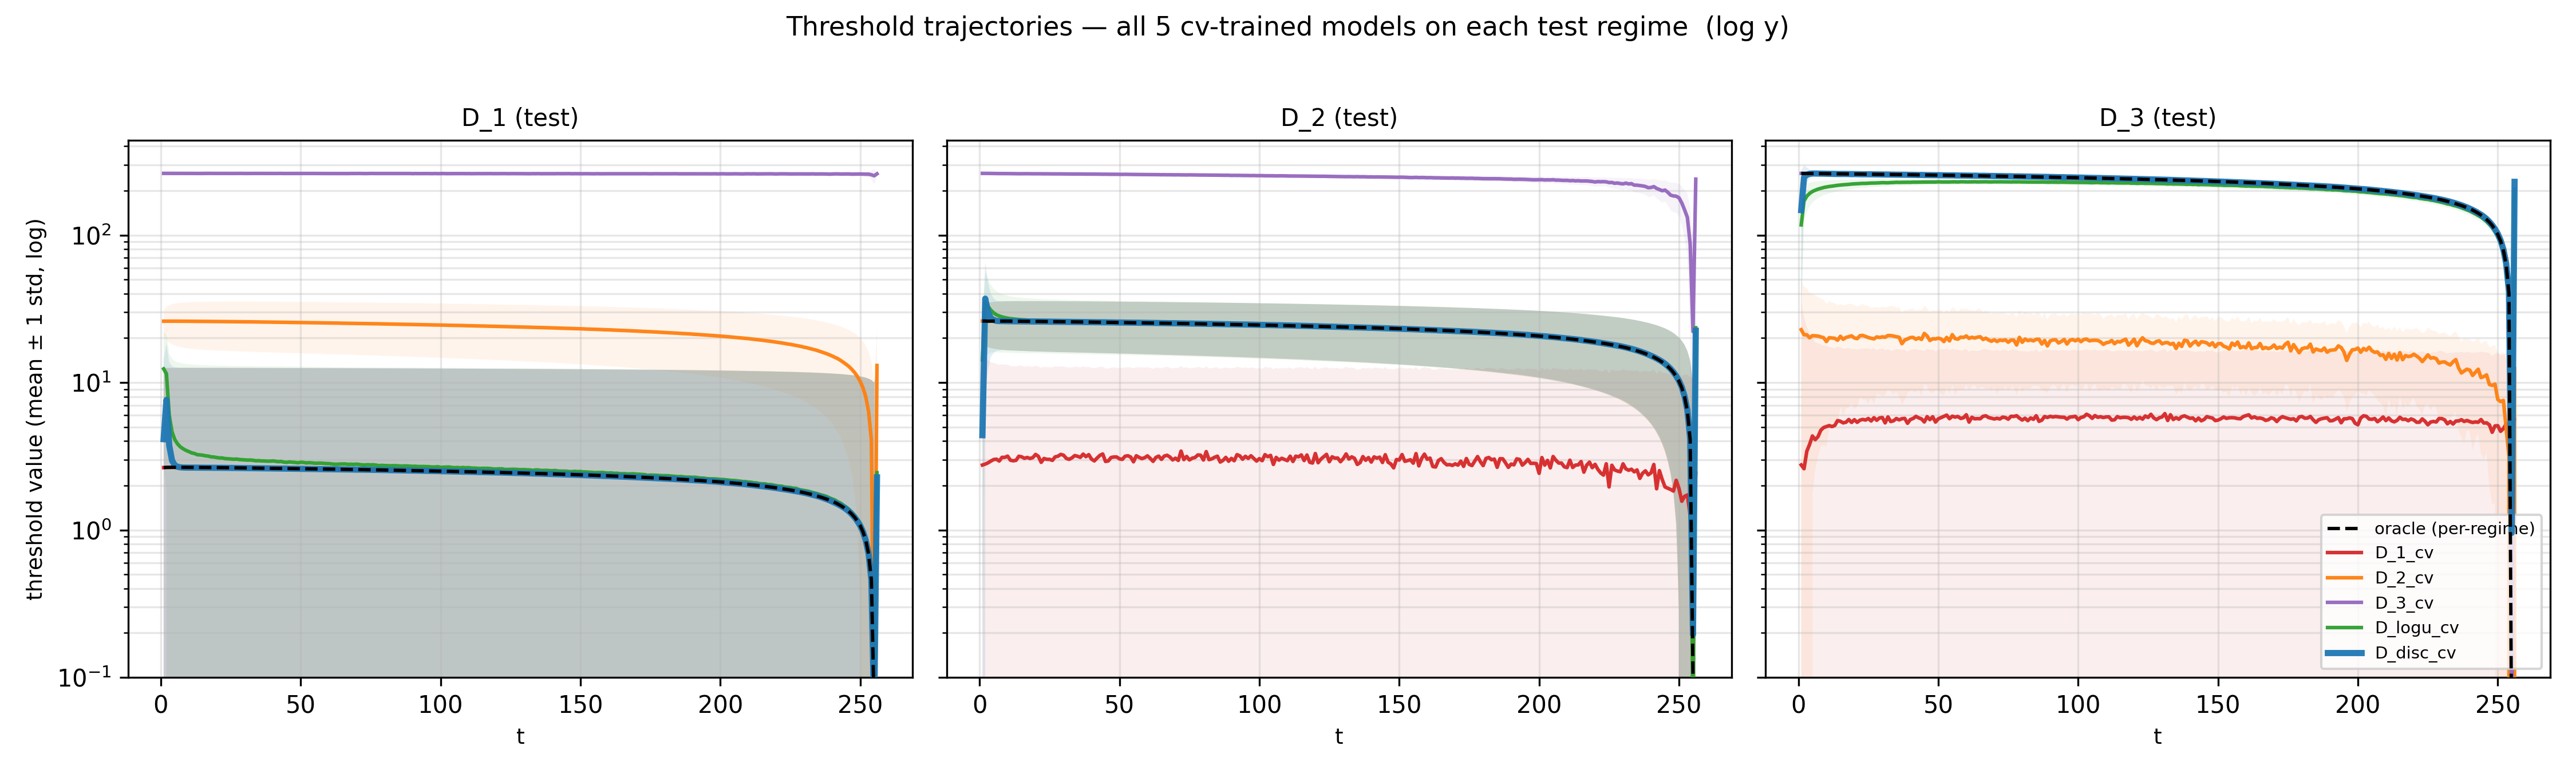
\includegraphics[width=\textwidth]{figures/trajectories-all-cv-log.png}
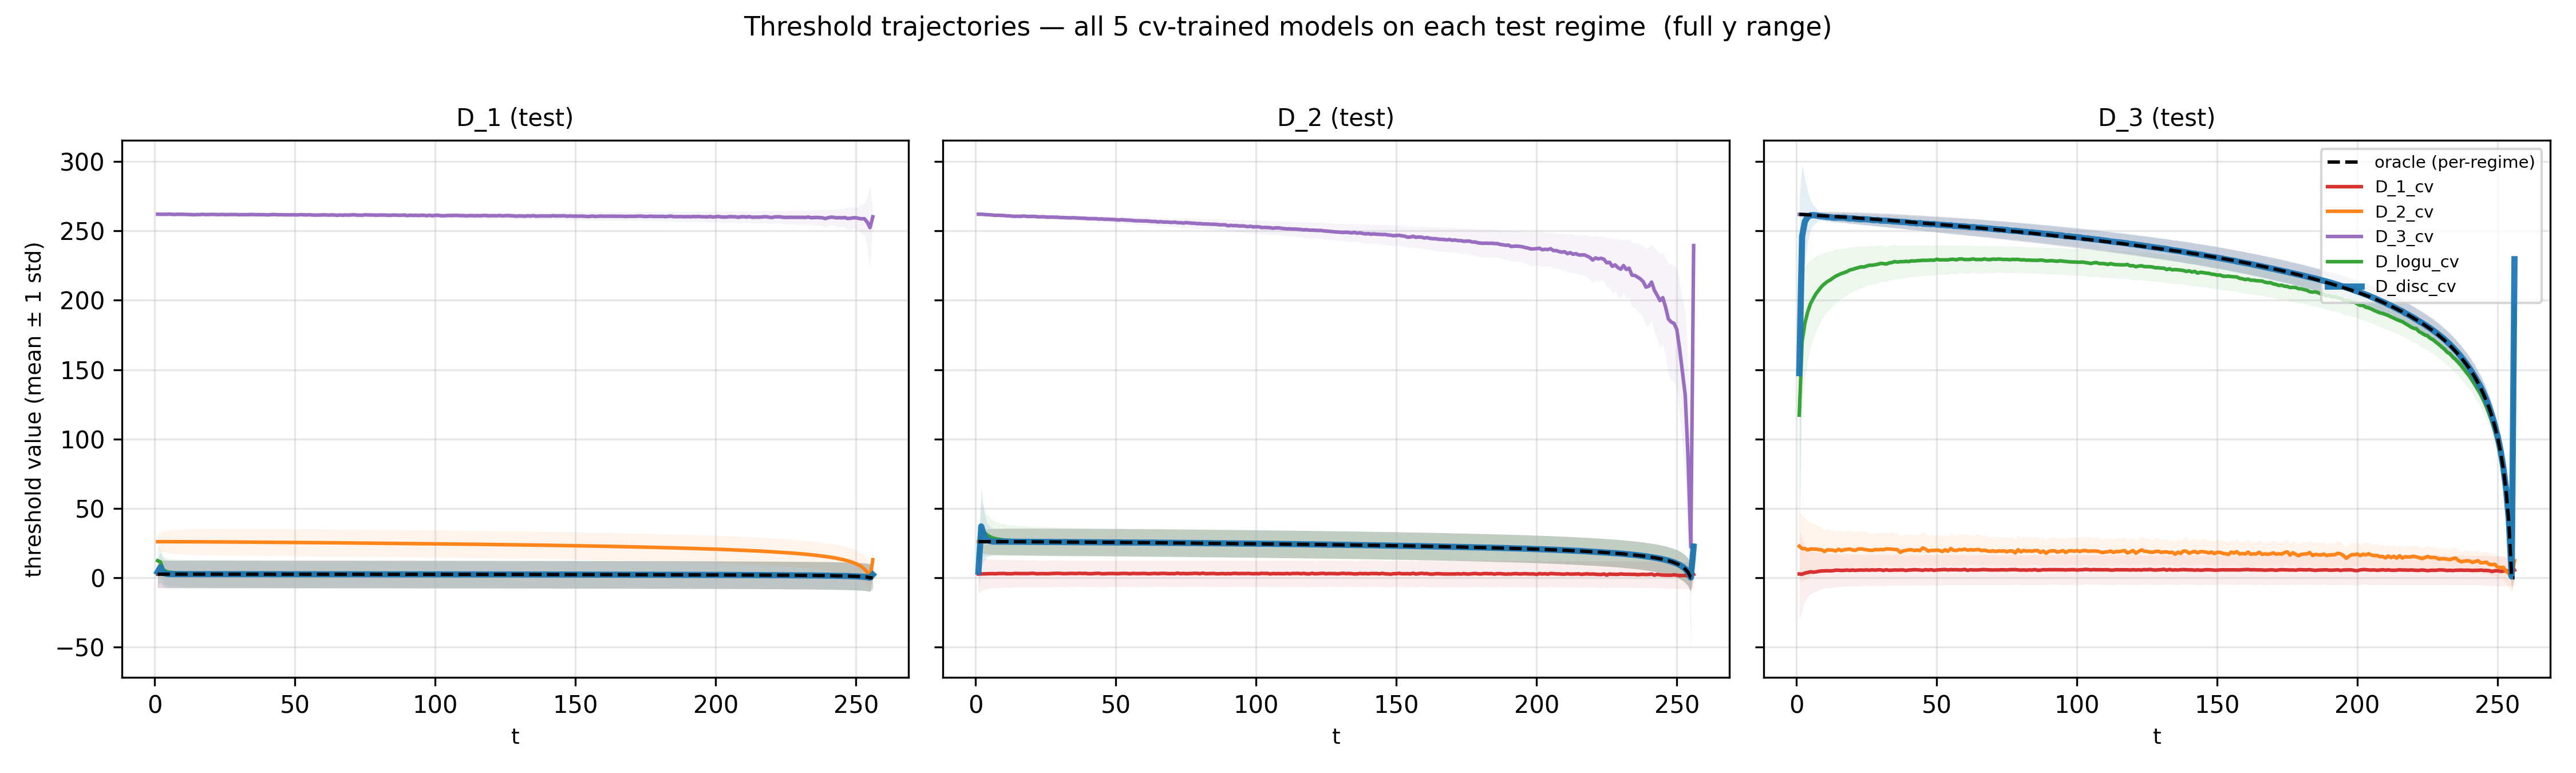
\includegraphics[width=\textwidth]{figures/trajectories-all-cv-full.png}
\caption{All five continuation-value-trained models overlaid on each test regime, with the per-regime oracle (black dashed) for reference. The three single-regime models ($\mathcal{D}_1$\_cv red, $\mathcal{D}_2$\_cv orange, $\mathcal{D}_3$\_cv purple) plateau at their training-distribution scale on every regime; the multi-regime models $\mathcal{D}_{\mathrm{disc}}$\_cv (blue) and $\mathcal{D}_{\mathrm{logu}}$\_cv (green) both track the per-regime oracle on each panel. Top: log y, negatives clipped. Bottom: linear y, full range (negative-side $\pm 1$ std bands shown).}
\label{fig:traj-all-cv}
\end{figure}

These single-regime results are exactly what the shortcut hypothesis predicts: each model applies one training-distribution-tuned threshold and ignores the test regime's noise level. With only one $\sigma$ in the training data, the optimizer had no incentive to learn a noise-conditional rule --- the experiment cannot tell us whether the architecture \emph{could} express one. To find out, we need a training distribution that forces it.

\subsection{Random-variance multi-regime success}
\label{sec:res-disc}

Training on a distribution over $\sigma$ is the natural test of the learning-algorithm hypothesis: no single threshold is Bayes-optimal across $\sigma \in \{1, 10, 100\}$, so matching the per-regime oracle on every test regime would imply that the network is inferring $\sigma$ in context and applying the corresponding rule. Both $\mathcal{D}_{\mathrm{disc}}$\_cv and $\mathcal{D}_{\mathrm{disc}}$\_act do exactly that (right four columns of Figure~\ref{fig:payoff-and-agreement}): $R/R^\star = 0.999, 0.999, 1.000$ for continuation-value supervision and $0.999, 0.999, 0.999$ for action supervision on $\mathcal{D}_1, \mathcal{D}_2, \mathcal{D}_3$. $\mathcal{D}_{\mathrm{logu}}$\_cv attains $R/R^\star = 0.972, 0.976, 0.973$ and $\mathcal{D}_{\mathrm{logu}}$\_act attains $0.974, 0.976, 0.975$ on the same three regimes; the gap between supervisions is below $0.005$ on every regime.

\begin{figure}[H]
\centering
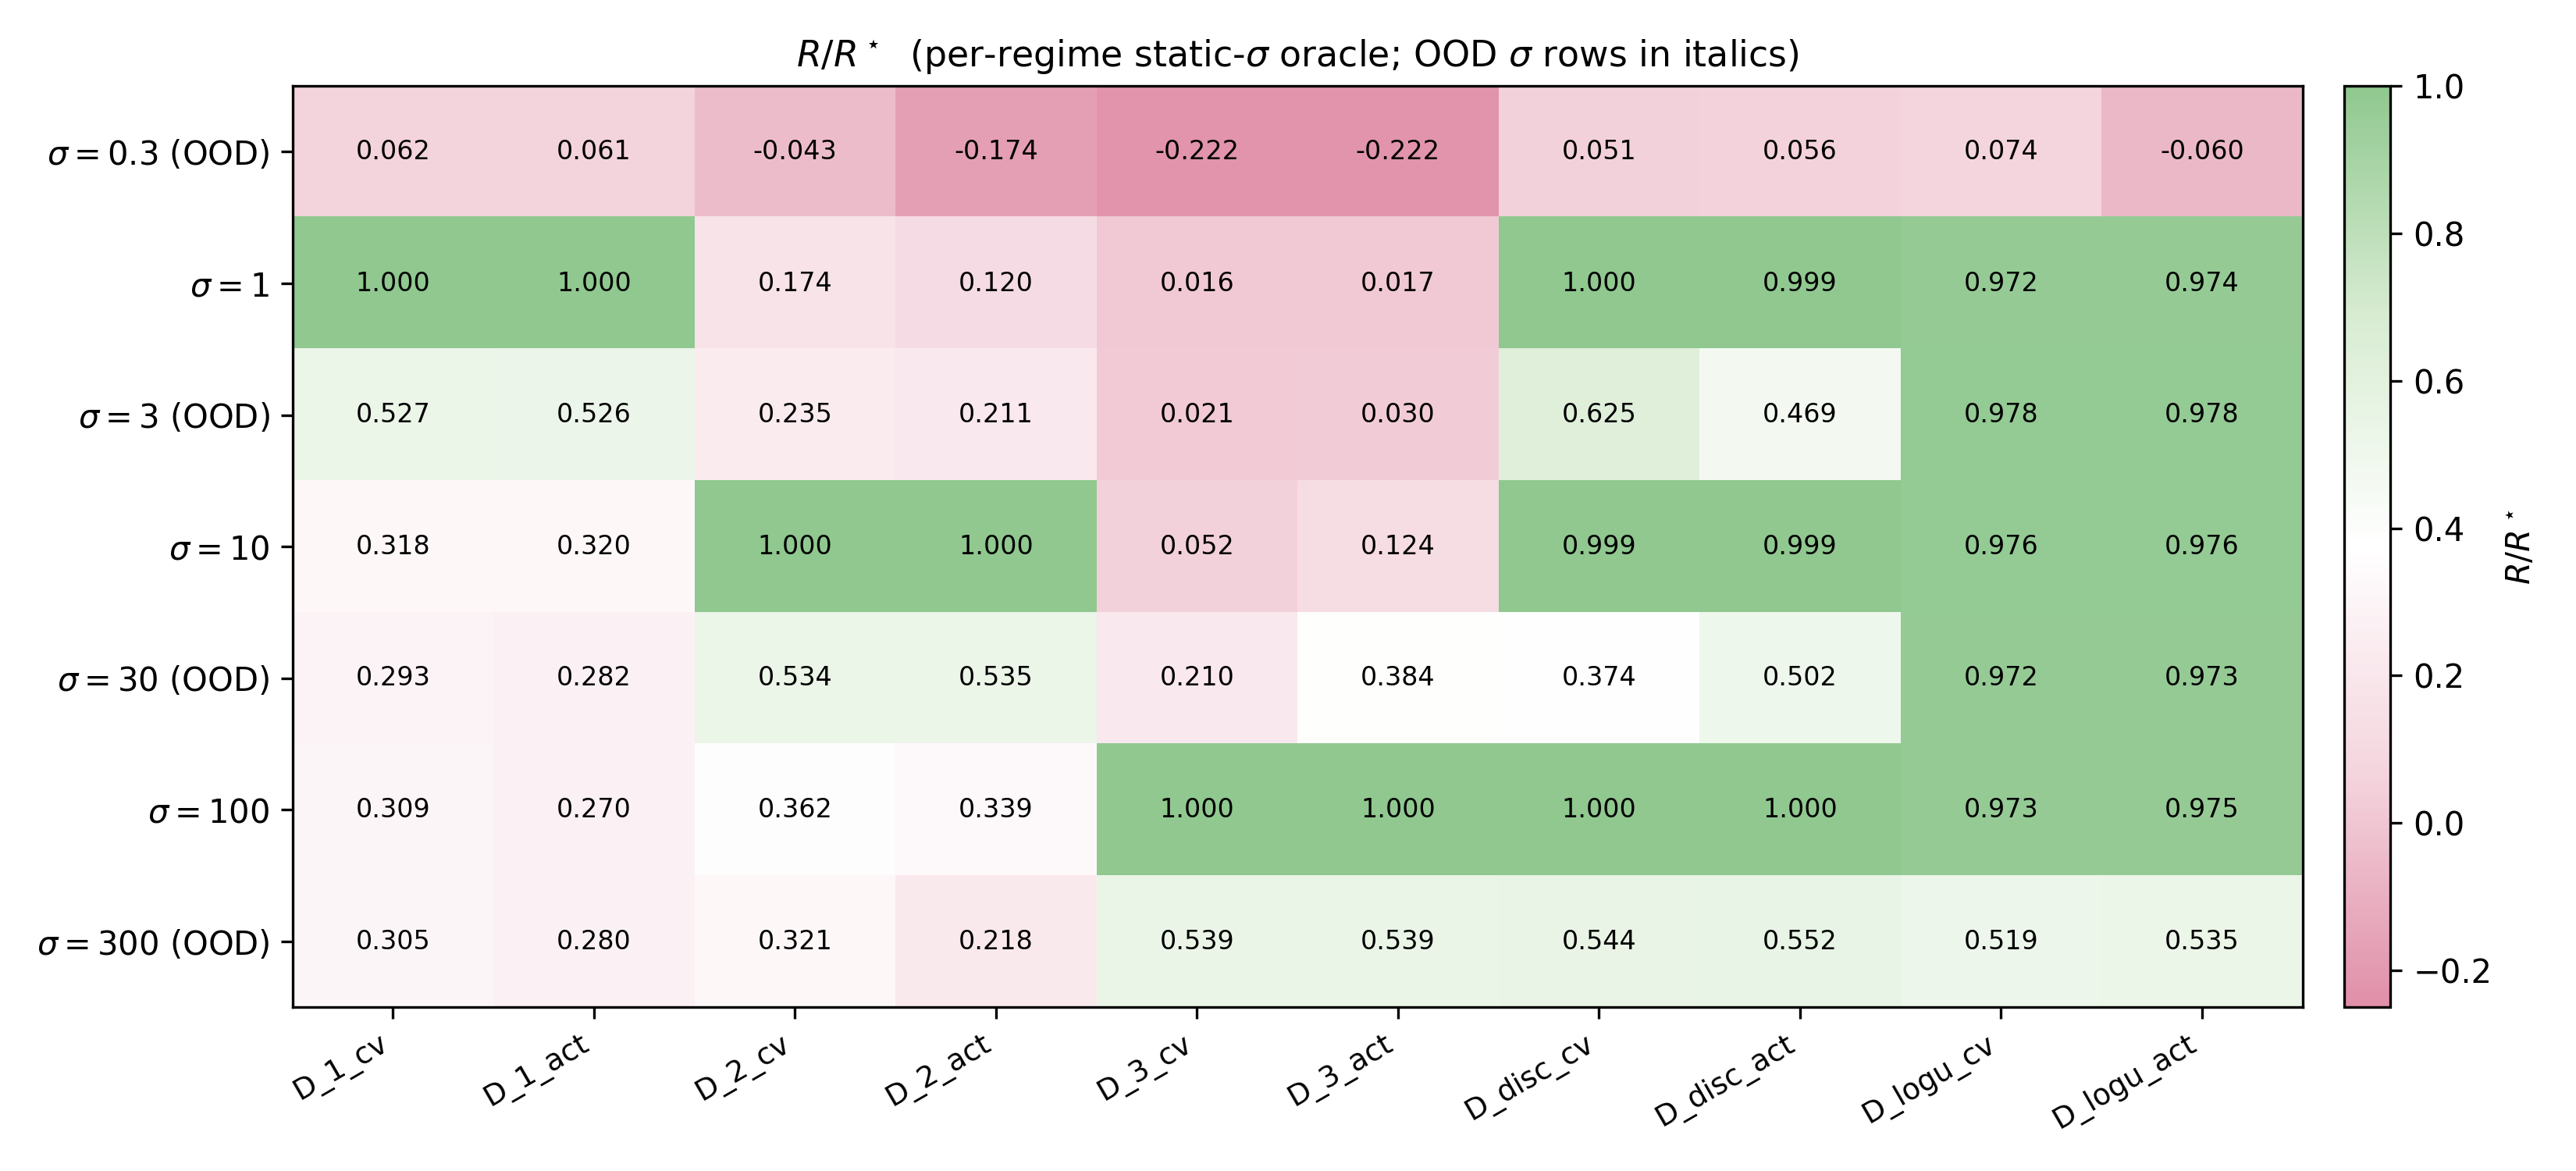
\includegraphics[width=0.92\textwidth]{figures/payoff-matrix-extended.png}
\caption{Competitive ratio $R/R^\star$ per (test regime, trained model): seven test regimes (rows; OOD in italics) $\times$ ten trained models (columns). Primary results figure for Section~\ref{sec:results}.}
\label{fig:payoff-and-agreement}
\end{figure}

We use $R/R^\star$ as the primary metric throughout the report. Per-step action agreement with the per-regime oracle is a tempting alternative, but it is misleading on its own --- $\mathcal{D}_3$\_cv on $\mathcal{D}_1$ agrees with the oracle on $97.8\%$ of decisions yet attains $R/R^\star = 0.016$. We report agreement only as a diagnostic; the heatmap and the full discussion are deferred to Appendix~\ref{sec:res-agreement}.

The per-$\sigma$ payoff breakdown confirms uniform competence across the training prior (Figure~\ref{fig:per-sigma-disc-logu}). For $\mathcal{D}_{\mathrm{disc}}$\_cv: $R/R^\star \in \{1.001, 0.999, 0.999\}$ at $\sigma \in \{1, 10, 100\}$; $\mathcal{D}_{\mathrm{disc}}$\_act is within $0.001$ of the oracle in every bin. For $\mathcal{D}_{\mathrm{logu}}$\_cv: $R/R^\star \in [0.999, 1.000]$ across all five $\log_{10}\sigma$ bins, indistinguishable from $\mathcal{D}_{\mathrm{logu}}$\_act.

\begin{figure}[H]
\centering
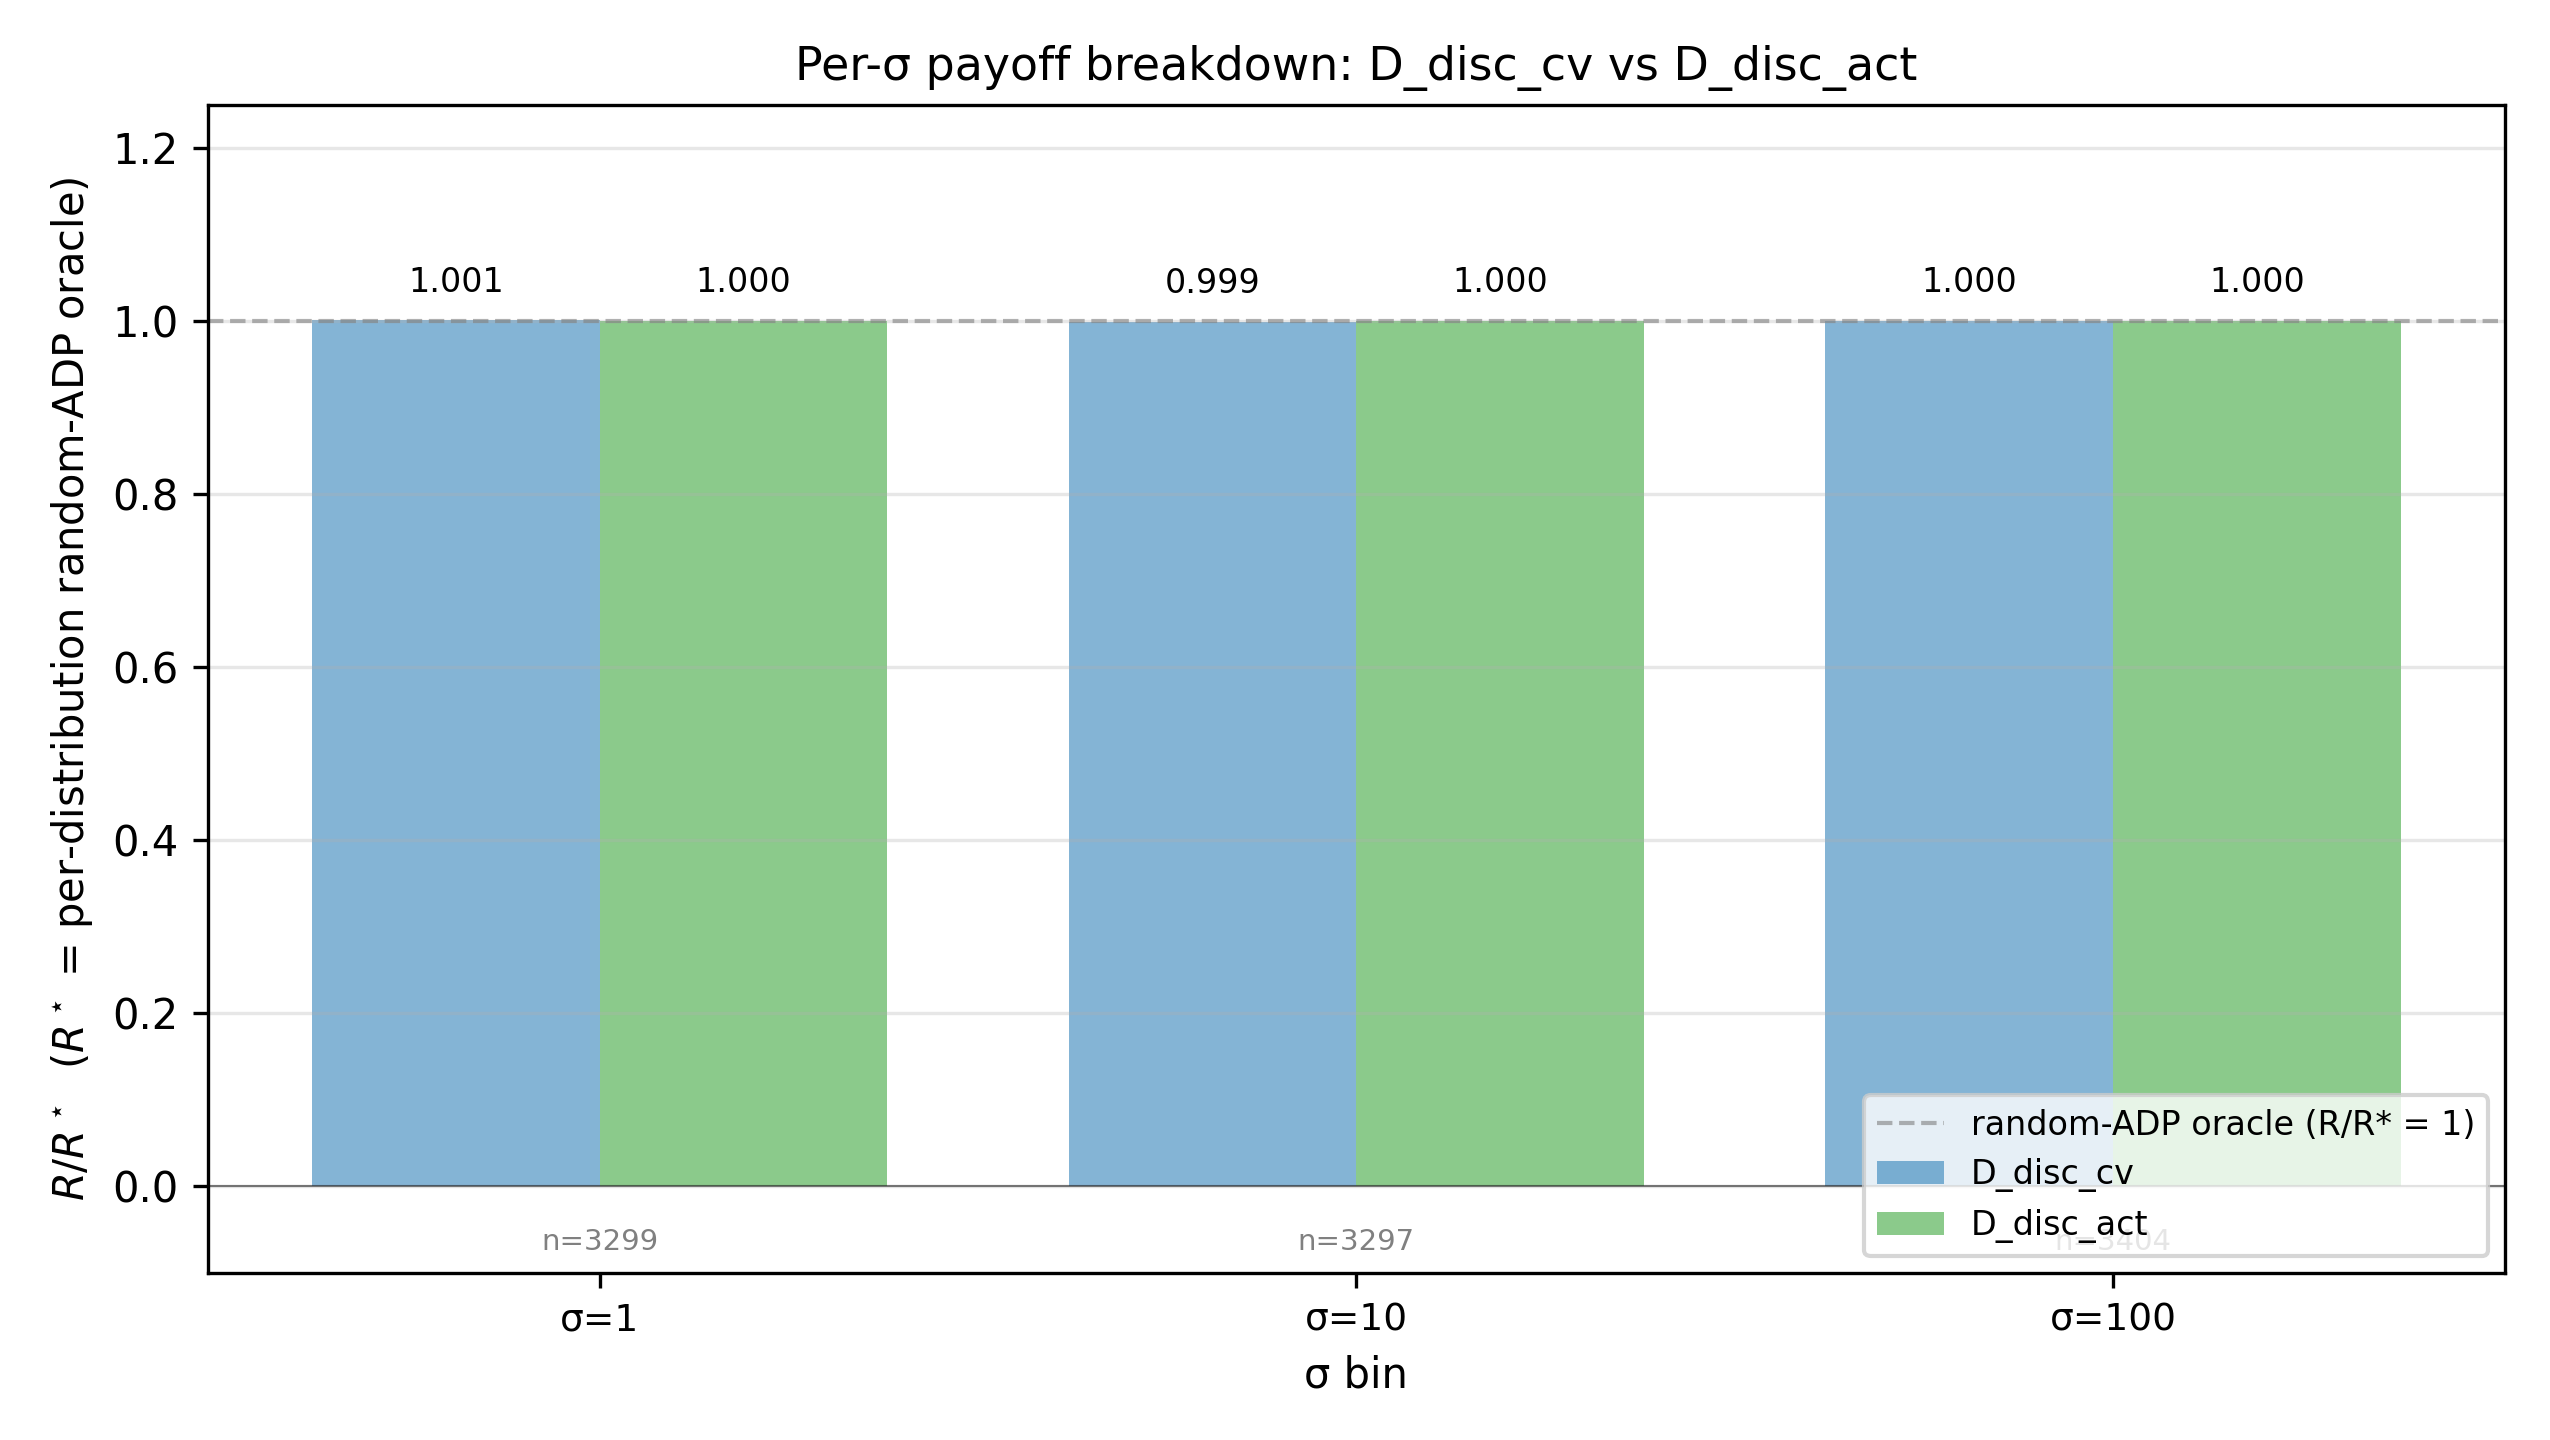
\includegraphics[width=0.49\textwidth]{figures/per-sigma-d-disc.png}\hfill
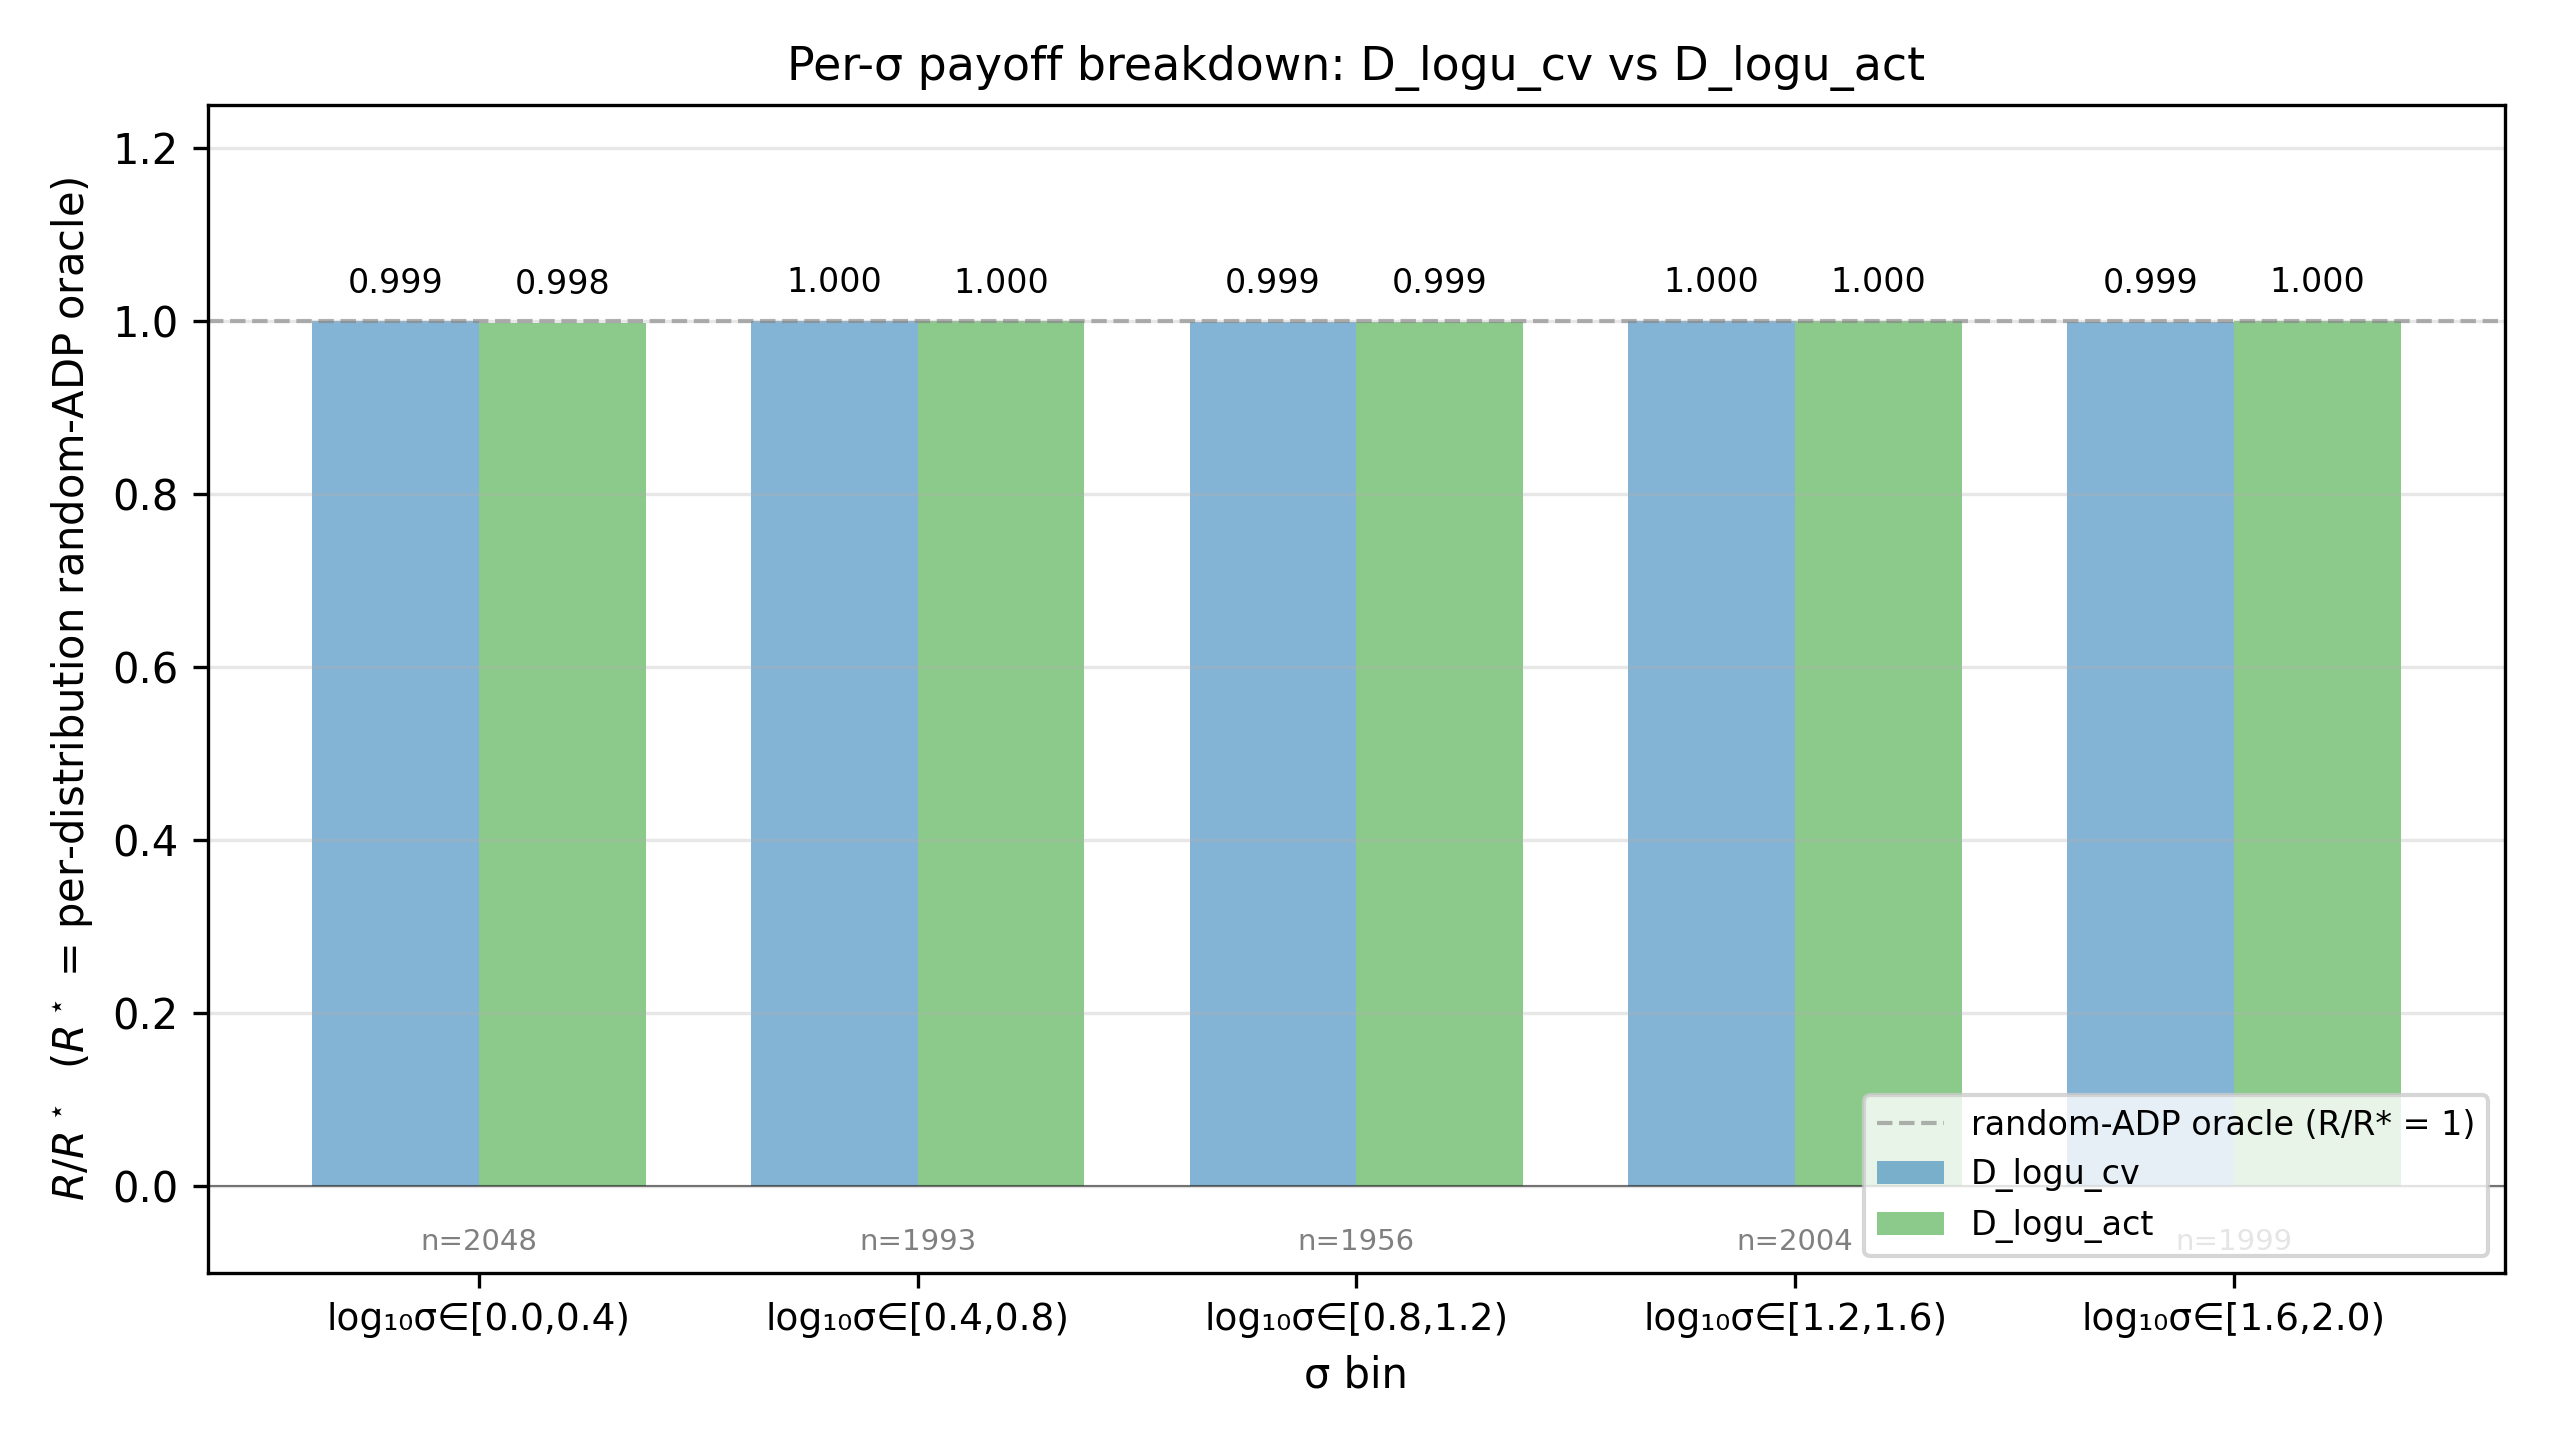
\includegraphics[width=0.49\textwidth]{figures/per-sigma-d-logu.png}
\caption{Per-$\sigma$ payoff breakdown. Left: $\mathcal{D}_{\mathrm{disc}}$\_cv (blue) vs.\ $\mathcal{D}_{\mathrm{disc}}$\_act (green). Right: $\mathcal{D}_{\mathrm{logu}}$\_cv vs.\ $\mathcal{D}_{\mathrm{logu}}$\_act. $R^\star =$ per-regime static-$\sigma$ oracle in both panels; both bracket the dashed $R/R^\star = 1$ reference in every $\sigma$ bin.}
\label{fig:per-sigma-disc-logu}
\end{figure}

The near-zero gap between action and continuation-value supervision in Figure~\ref{fig:per-sigma-disc-logu} is itself notable. Action supervision is a strictly lower-signal target: a binary $\{0, 1\}$ label tells the model only whether to stop, not by how much --- it carries no information about how close the current observation is to the optimal threshold or how ``bad'' a wrong call would be. The action-supervised models nonetheless match the continuation-value counterparts in payoff, which suggests that they reconstruct a continuation-value-like representation internally from the binary labels alone. We test this directly in Section~\ref{sec:probe} by probing whether $\widehat C^\star_t$ is linearly decodable from the action-supervised models' hidden states, even though $\widehat C^\star_t$ never appears in their training loss.

The threshold trajectories (Figures~\ref{fig:traj-disc-cv}--\ref{fig:traj-zoom}) show the corresponding signature: on each test regime the model's threshold moves toward the per-regime oracle within a few observations of $X_t$ and tracks it for the remainder of the horizon. The model is performing in-context $\sigma$ inference and applying the regime-corresponding threshold rule.

\begin{figure}[H]
\centering
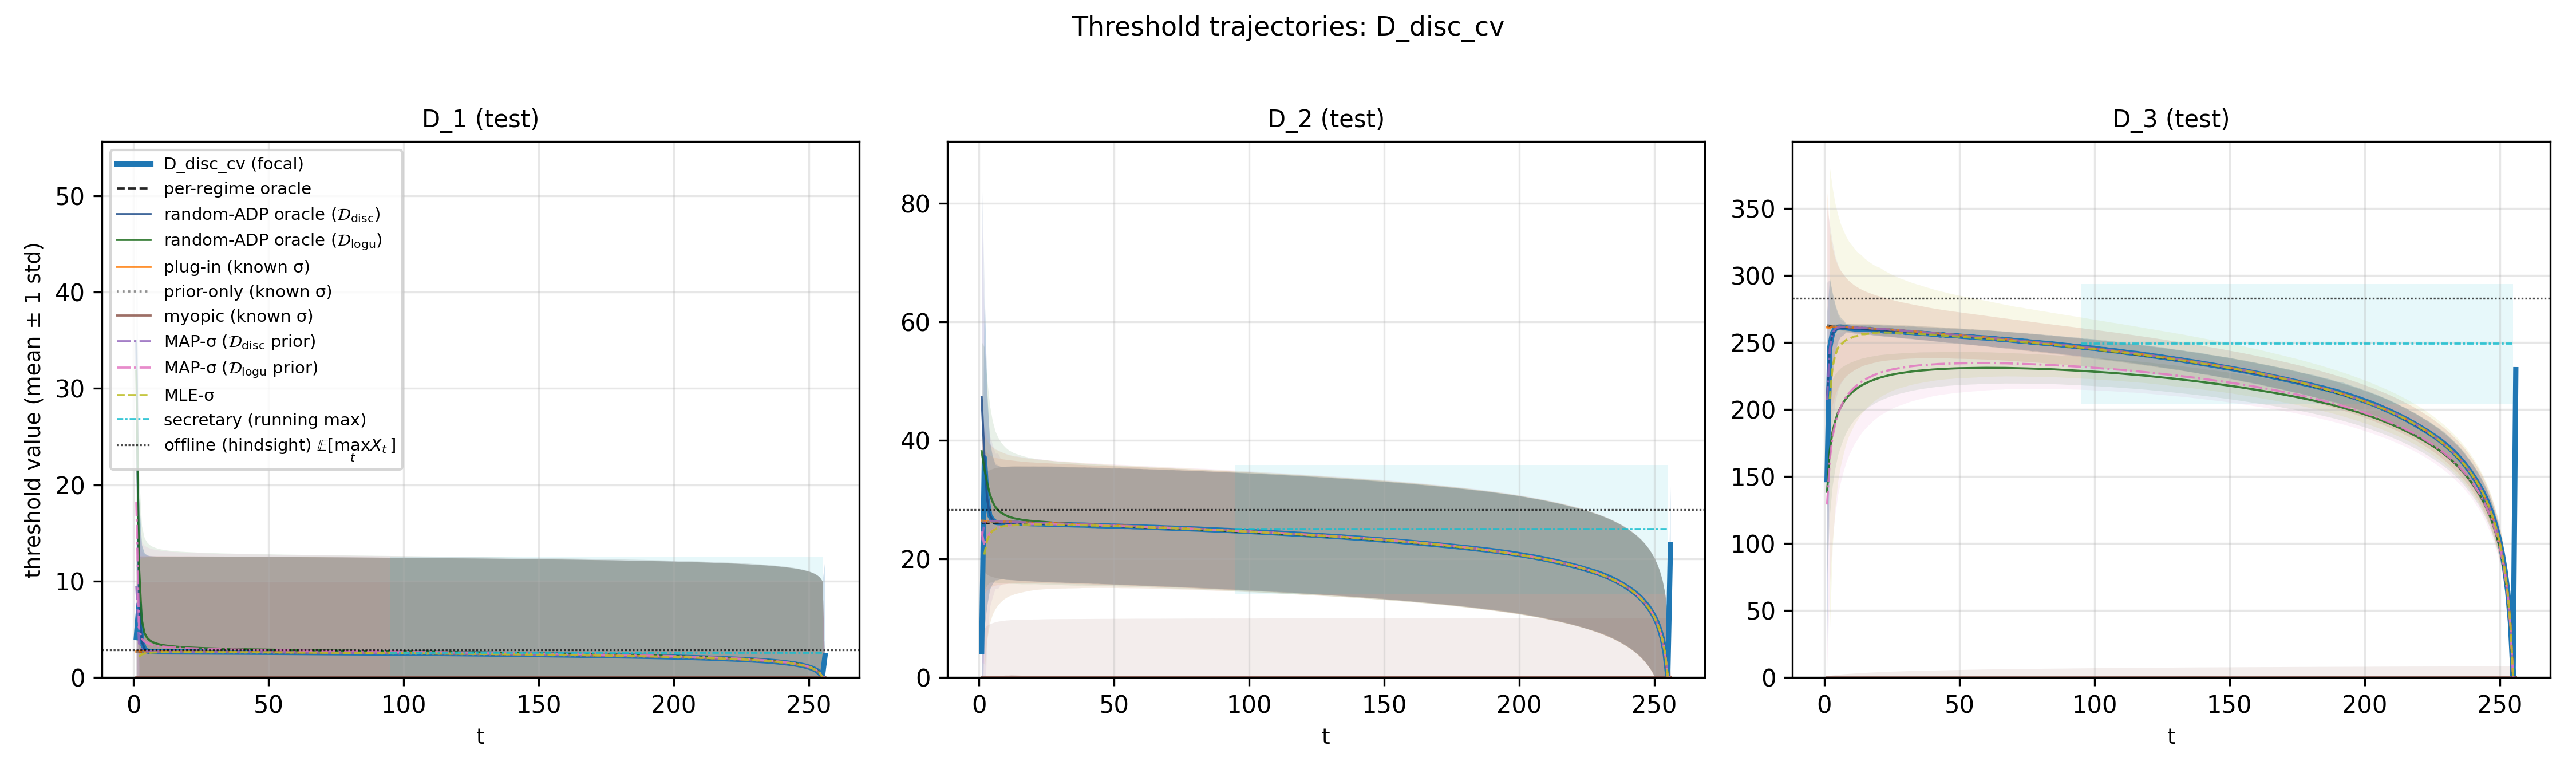
\includegraphics[width=\textwidth]{figures/trajectories-d-disc-cv.png}
\caption{Threshold trajectory for $\mathcal{D}_{\mathrm{disc}}$\_cv (focal, blue, mean $\pm 1$ std band) on each in-distribution test regime, with all baselines from Section~\ref{sec:baselines} overlaid. The model adapts to the test regime within a few observations and tracks the per-regime oracle (black dashed) and the $\mathcal{D}_{\mathrm{disc}}$ random-ADP oracle for the remainder of the horizon on every regime.}
\label{fig:traj-disc-cv}
\end{figure}

\begin{figure}[H]
\centering
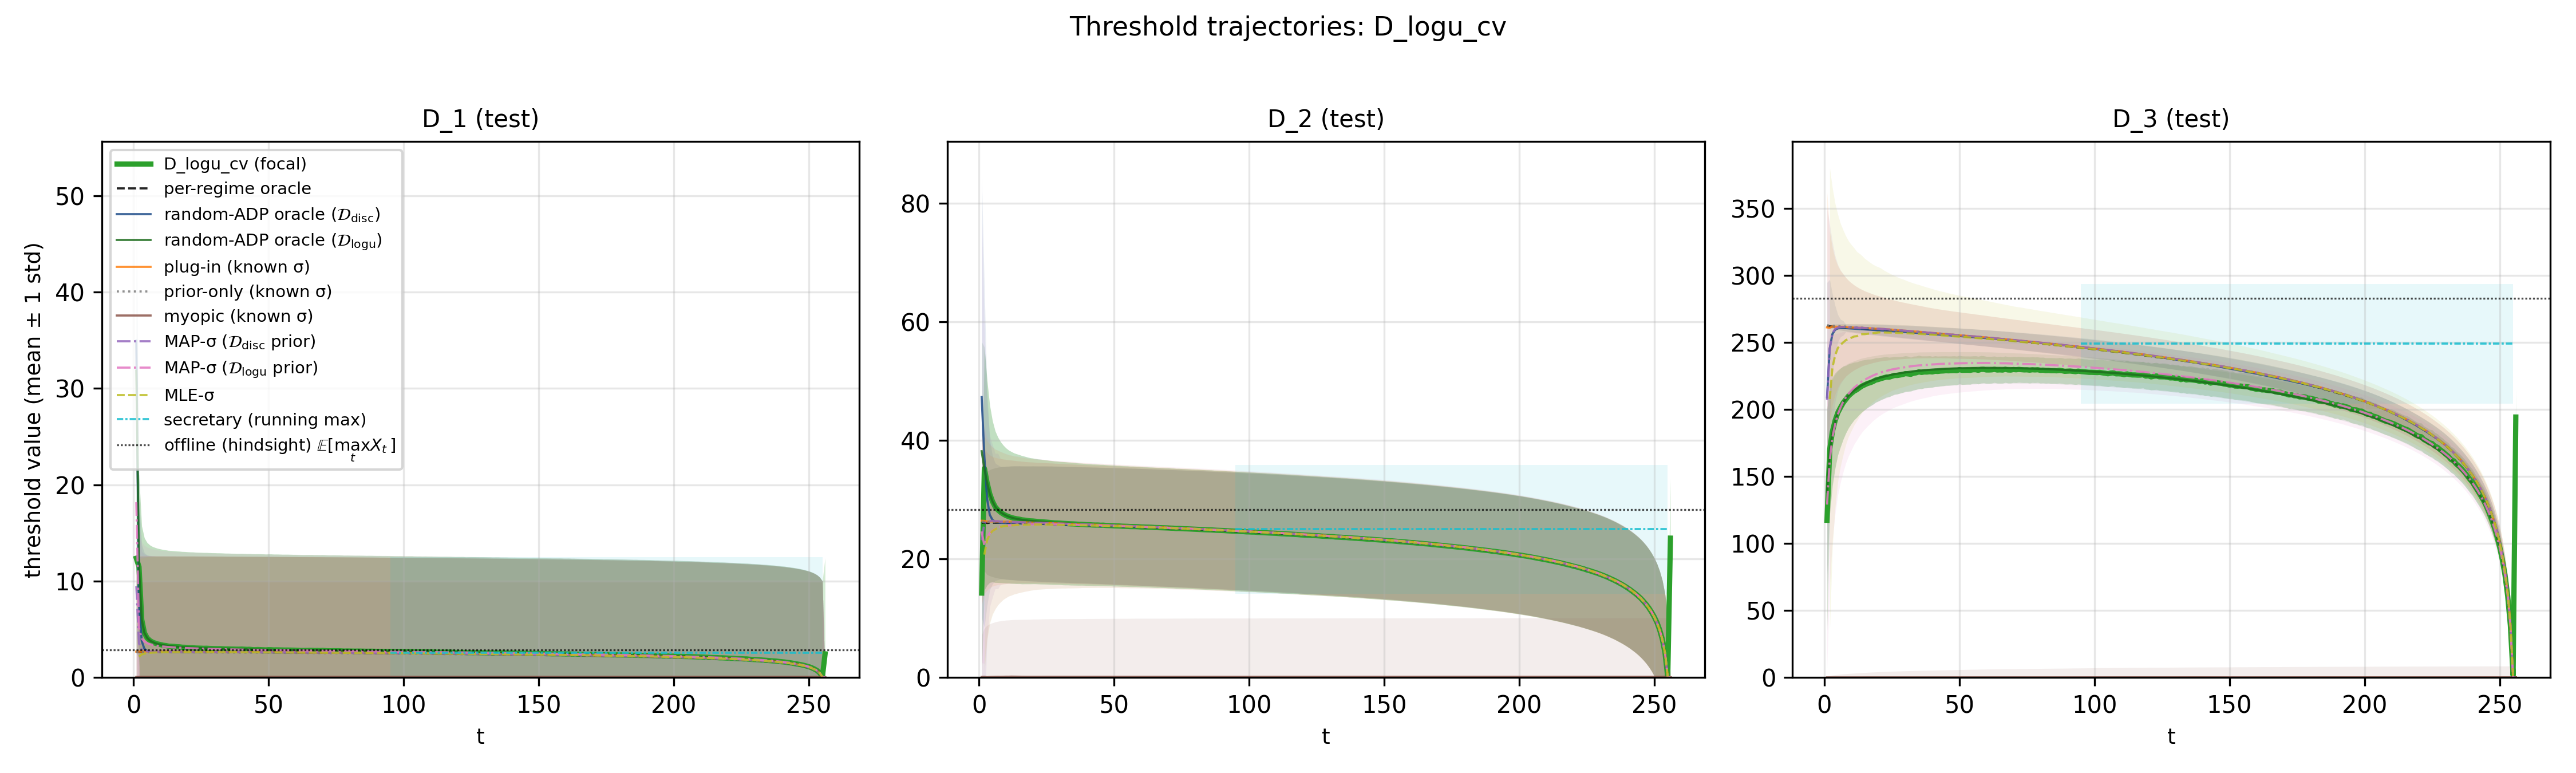
\includegraphics[width=\textwidth]{figures/trajectories-d-logu-cv.png}
\caption{Threshold trajectory for $\mathcal{D}_{\mathrm{logu}}$\_cv on each in-distribution test regime.}
\label{fig:traj-logu-cv}
\end{figure}

\begin{figure}[H]
\centering
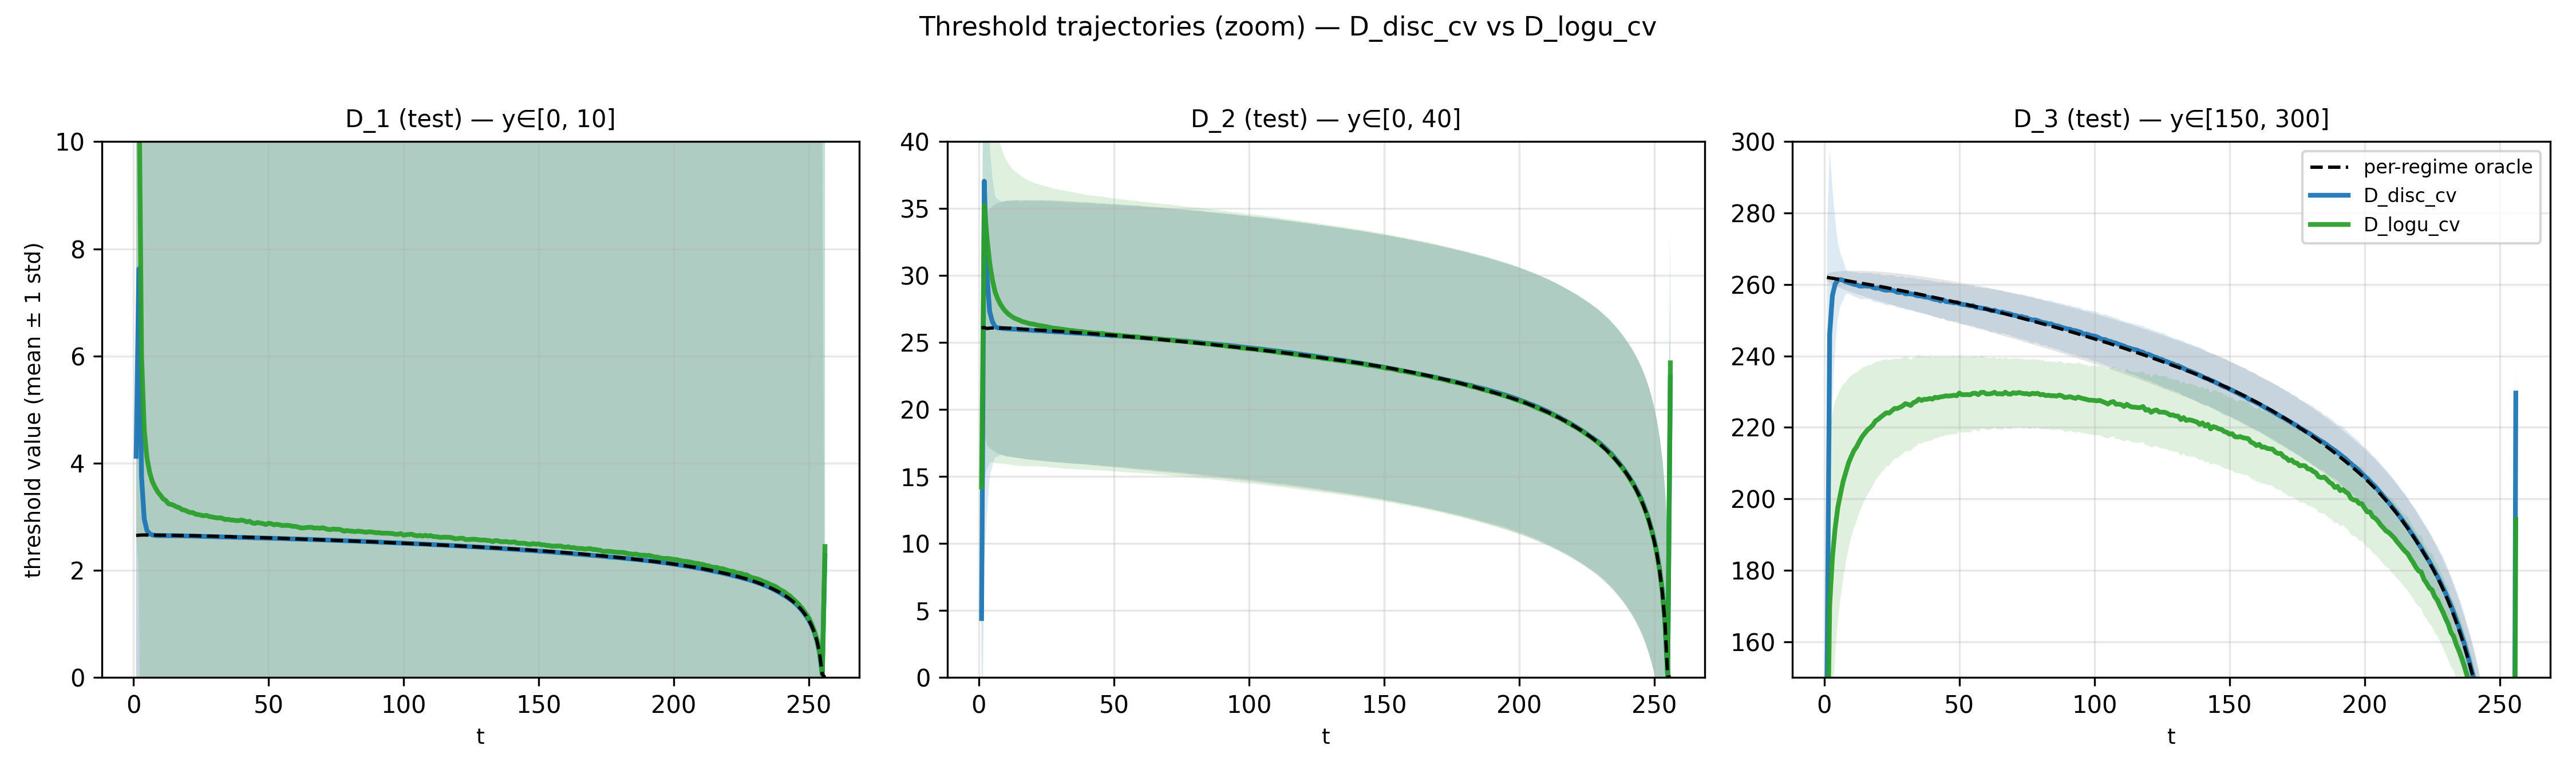
\includegraphics[width=\textwidth]{figures/trajectories-disc-logu-zoom.png}
\caption{Zoomed comparison of $\mathcal{D}_{\mathrm{disc}}$\_cv and $\mathcal{D}_{\mathrm{logu}}$\_cv against the per-regime oracle (black dashed) on each test regime, with per-panel y-limits: $y \in [0, 10]$ on $\mathcal{D}_1$, $[0, 40]$ on $\mathcal{D}_2$, $[150, 300]$ on $\mathcal{D}_3$.}
\label{fig:traj-zoom}
\end{figure}

\begin{figure}[H]
\centering
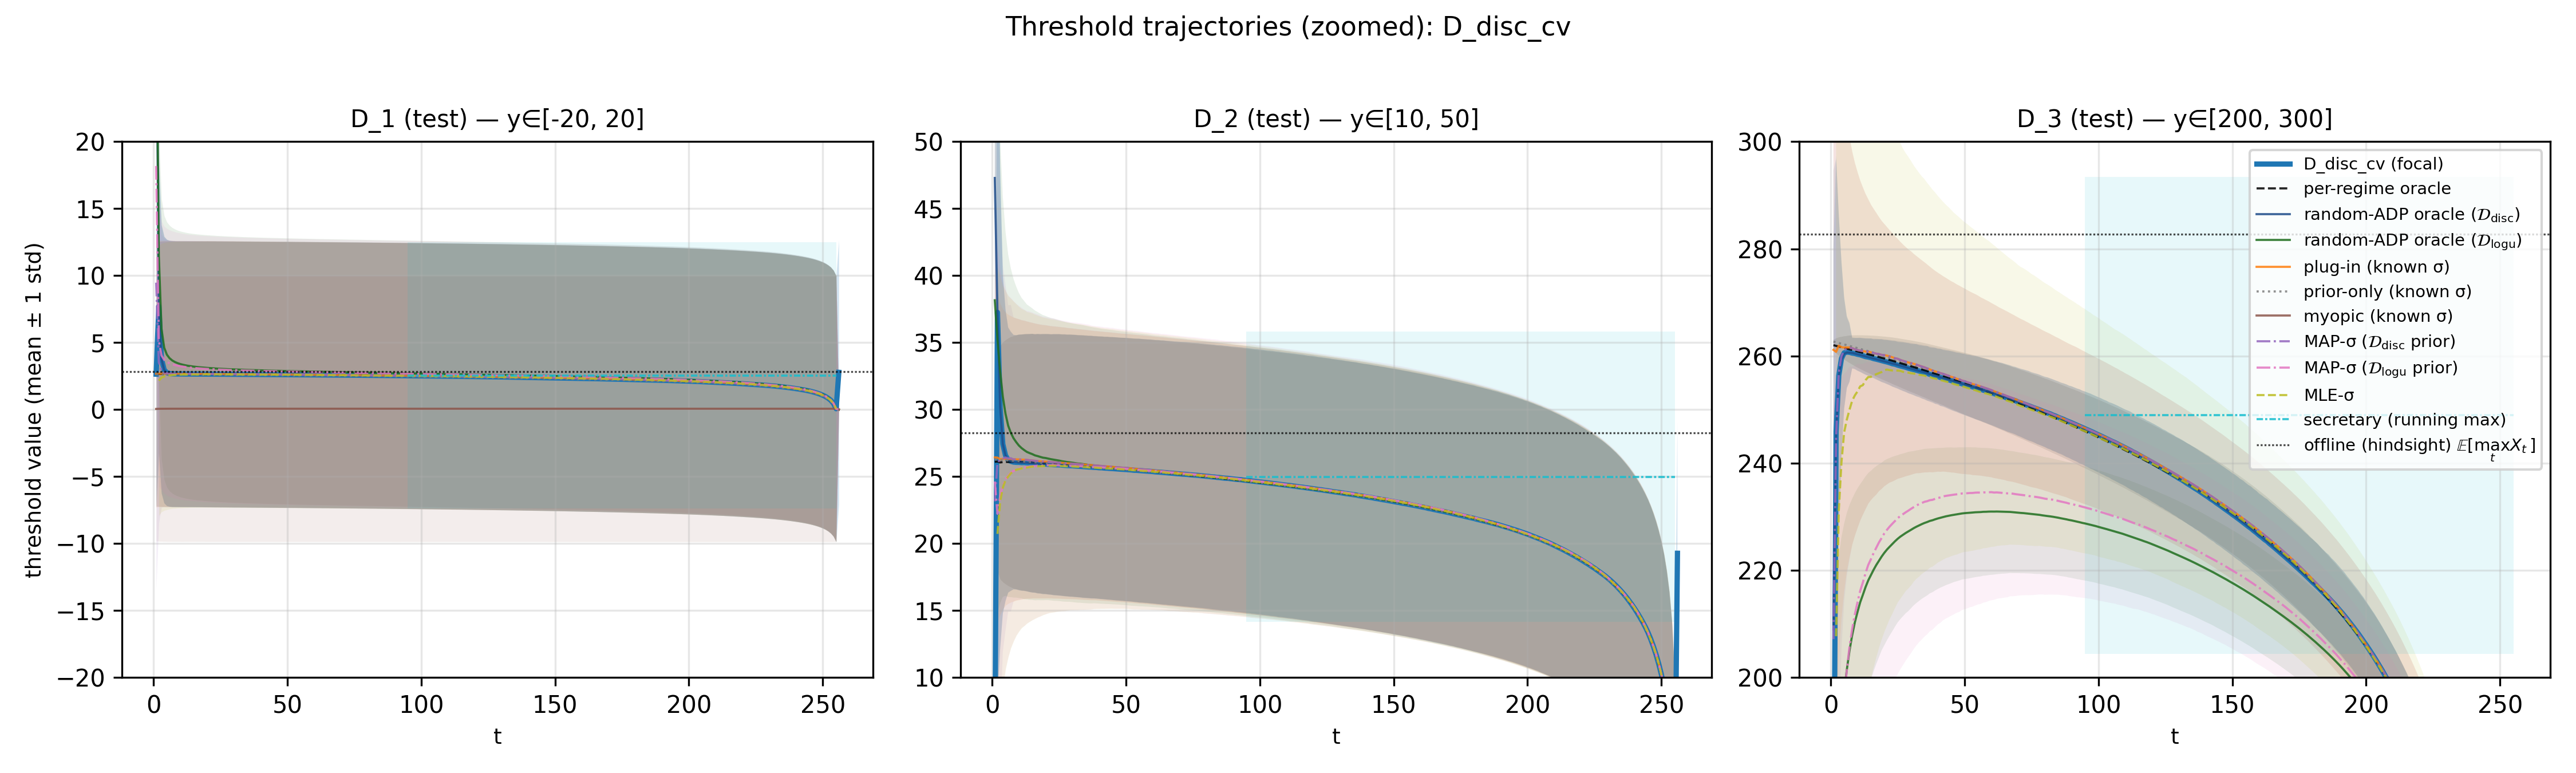
\includegraphics[width=\textwidth]{figures/trajectories-d-disc-cv-zoomed.png}
\caption{Per-panel zoomed threshold trajectory for $\mathcal{D}_{\mathrm{disc}}$\_cv against every baseline. Each panel uses a regime-specific y-window: $y \in [-20, 20]$ on $\mathcal{D}_1$, $[10, 50]$ on $\mathcal{D}_2$, $[200, 300]$ on $\mathcal{D}_3$.}
\label{fig:traj-disc-cv-zoomed}
\end{figure}

\begin{figure}[H]
\centering
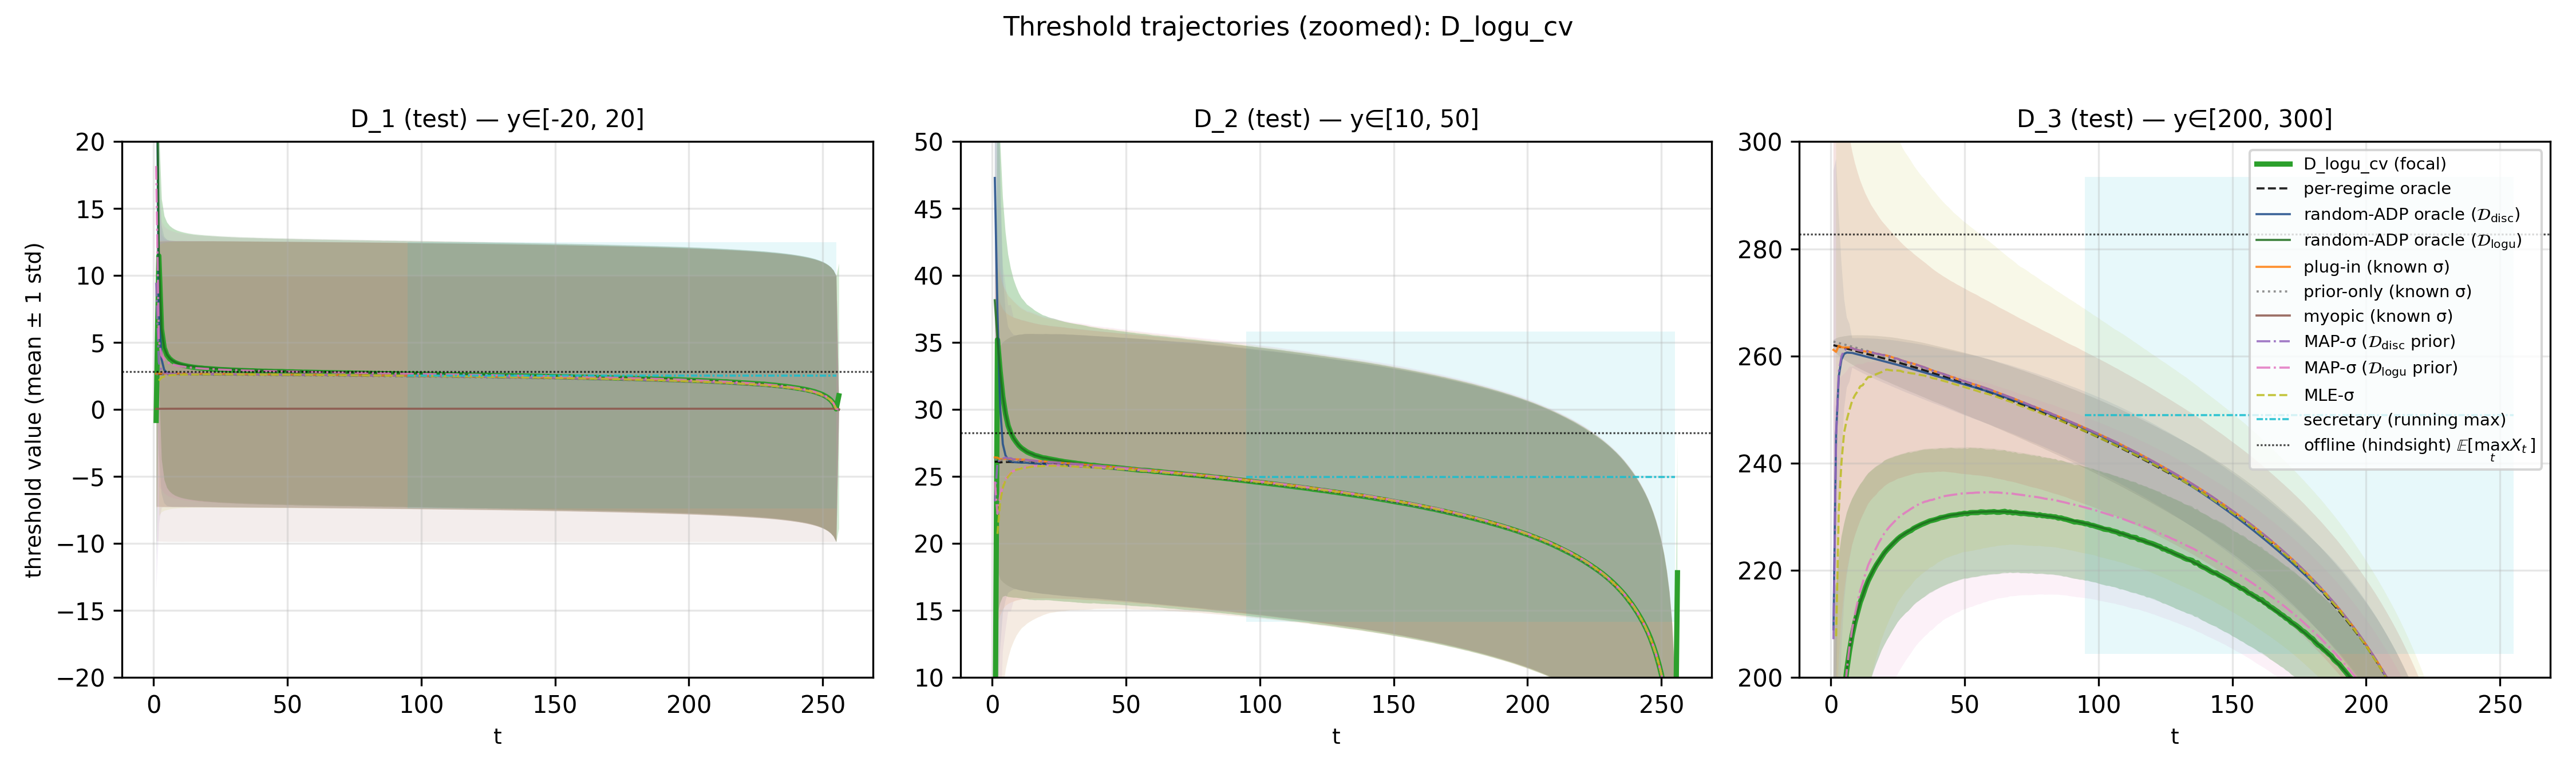
\includegraphics[width=\textwidth]{figures/trajectories-d-logu-cv-zoomed.png}
\caption{Per-panel zoomed threshold trajectory for $\mathcal{D}_{\mathrm{logu}}$\_cv against every baseline, same per-regime y-windows as Figure~\ref{fig:traj-disc-cv-zoomed}.}
\label{fig:traj-logu-cv-zoomed}
\end{figure}

\subsection{OOD on $\sigma$: interpolation beyond the training prior}
\label{sec:res-ood}

A noise-conditional rule should produce sensible thresholds not only at the training $\sigma$ values but at novel $\sigma$ as well. We test this with four OOD test regimes at $\sigma \in \{0.3, 3, 30, 300\}$ --- two interpolation points between $\mathcal{D}_{\mathrm{disc}}$'s training values $\{1, 10, 100\}$, two extrapolation points outside the support of both random-variance priors. Test caches at $N_{\mathrm{test}} = 10^4$ sequences each (disjoint seeds); per-regime static-$\sigma$ oracle tables solved via Algorithm~\ref{alg:adp-static} at $(K, J) = (2048, 128)$ and verified against the $(4096, 256)$ reference (action-label disagreement $\sim 3 \times 10^{-5}$ for every regime; combined seven-row diagnostic in Appendix~\ref{app:convergence}). All evaluations use existing trained checkpoints.

On the two interpolation points, $\mathcal{D}_{\mathrm{disc}}$\_cv attains $R/R^\star = 0.625$ at $\sigma = 3$ and $0.374$ at $\sigma = 30$, beating both the random-ADP oracle at the matching $\mathcal{D}_{\mathrm{disc}}$ prior ($0.244$ and $0.229$) and the matched MAP-$\sigma$ plug-in ($0.260$ and $0.243$) by $1.6\times$ to $2.5\times$ in $R/R^\star$ (Figure~\ref{fig:per-sigma-disc-extended}). The random-ADP-disc baseline is the Bayes-optimal policy under the discrete training prior, so $\mathcal{D}_{\mathrm{disc}}$\_cv exceeding it on novel $\sigma$ means the trained model is not limited to the prior's discrete support. On $\sigma \in \{3, 30\}$, both $\mathcal{D}_{\mathrm{logu}}$\_cv and $\mathcal{D}_{\mathrm{logu}}$\_act match MAP-$\sigma$ at the $\mathcal{D}_{\mathrm{logu}}$ prior to four decimal places. At extrapolation $\sigma = 300$ every trained model and the matching random-ADP oracle land in the $0.50$--$0.55$ band; at $\sigma = 0.3$ the trained random-variance models collapse near zero.

\begin{figure}[H]
\centering
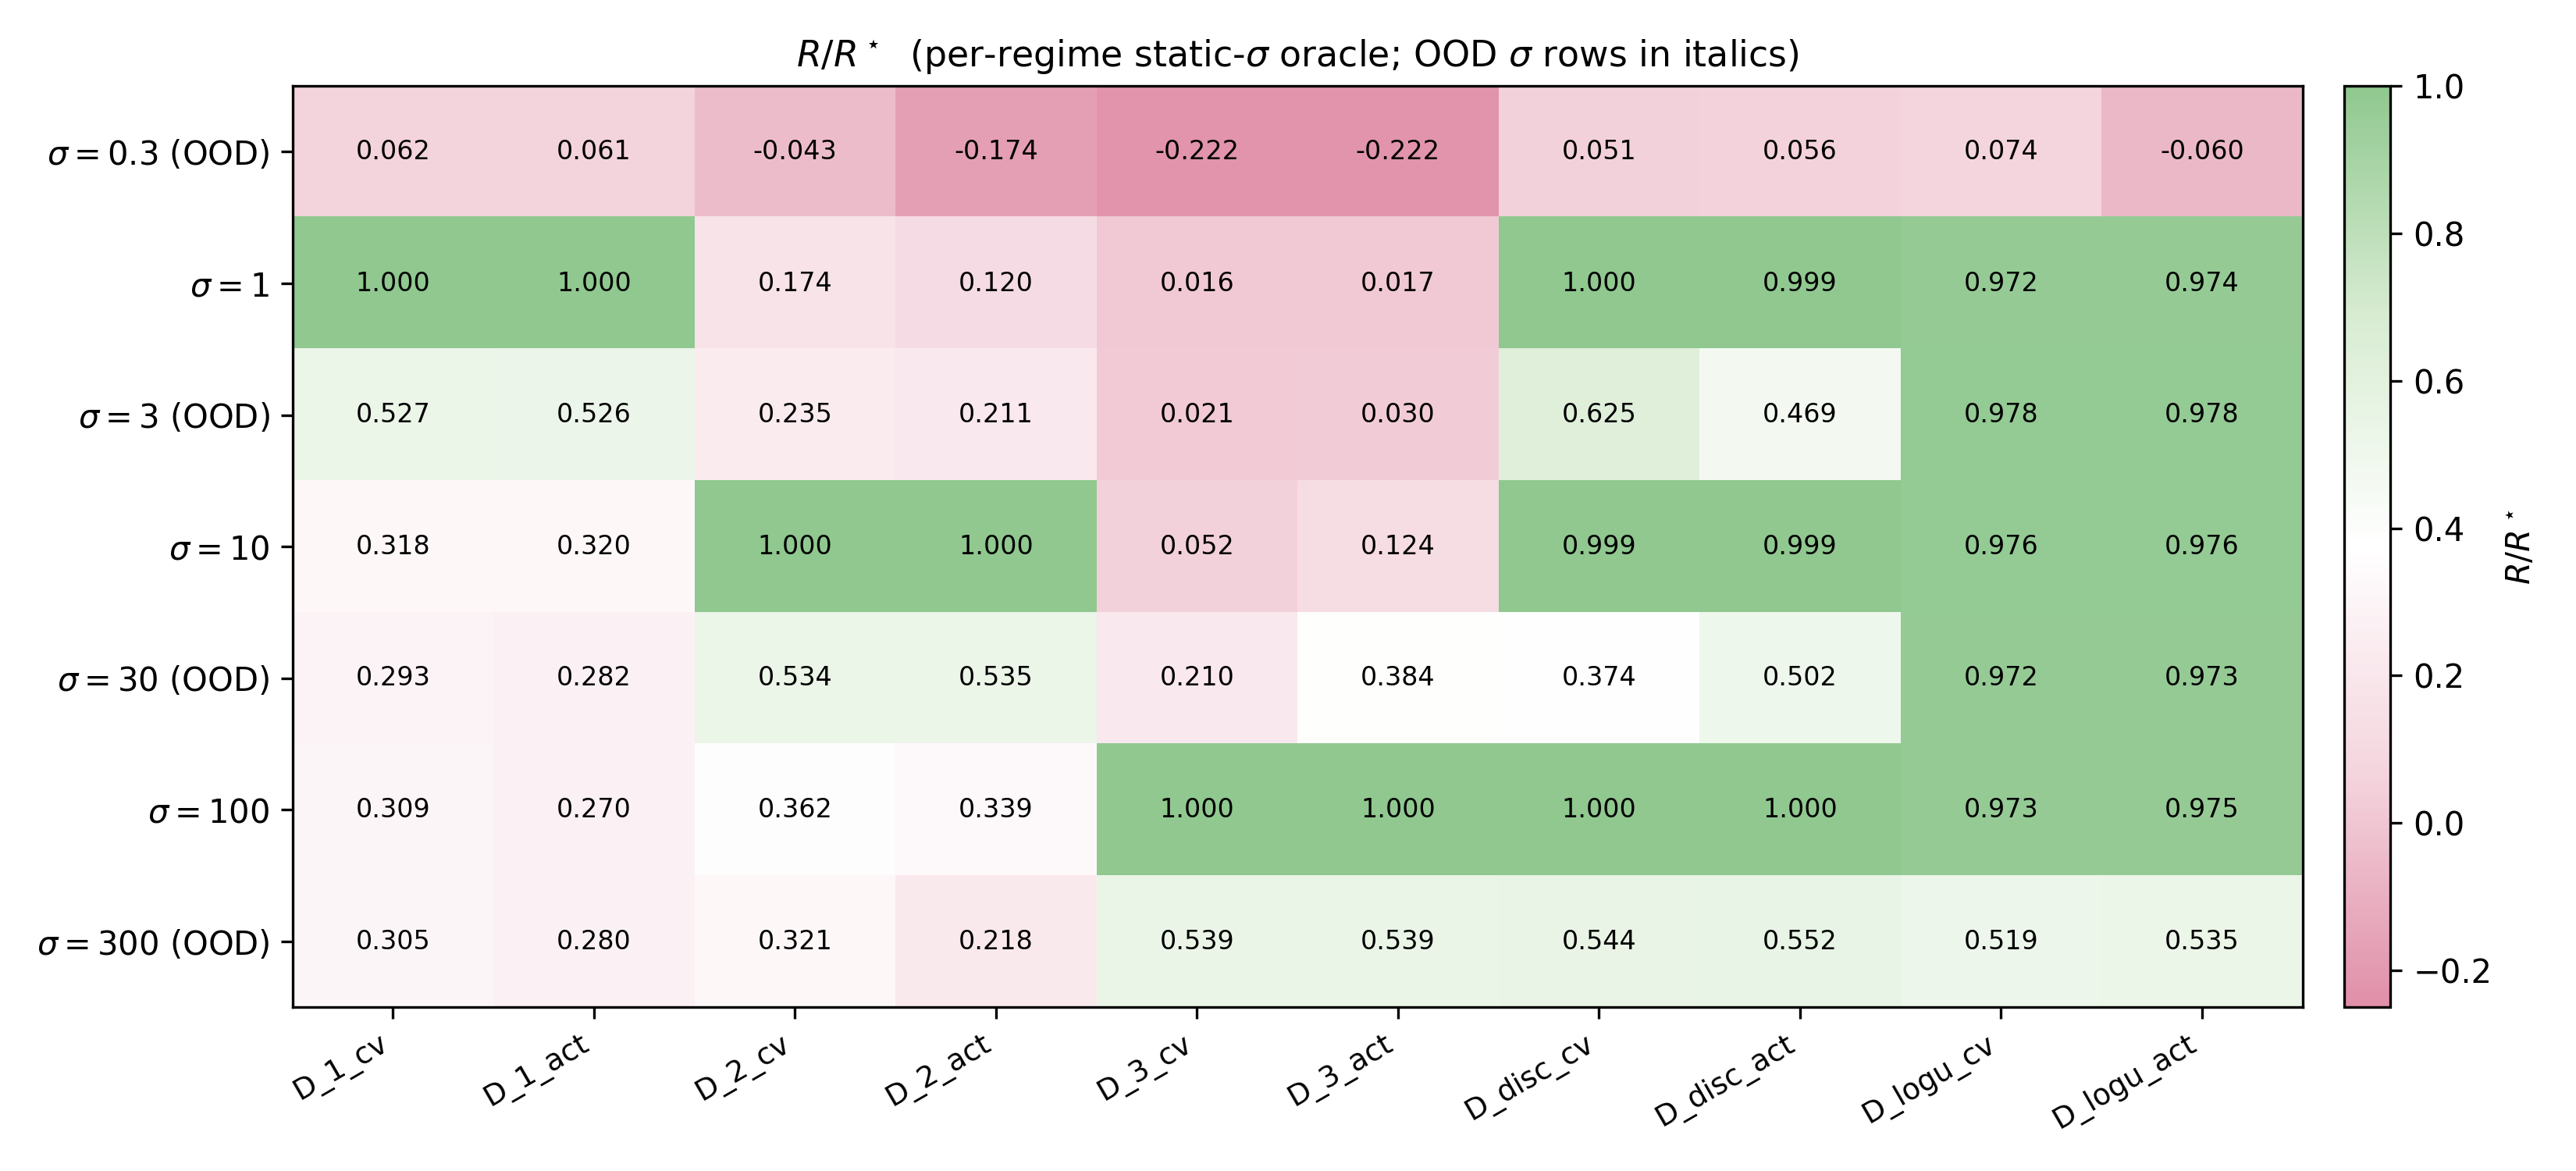
\includegraphics[width=\textwidth]{figures/payoff-matrix-extended.png}
\caption{Extended $R/R^\star$ heatmap. Seven test regimes (rows, in italics for OOD), ten trained models (columns).}
\label{fig:payoff-matrix-extended}
\end{figure}

\begin{figure}[H]
\centering
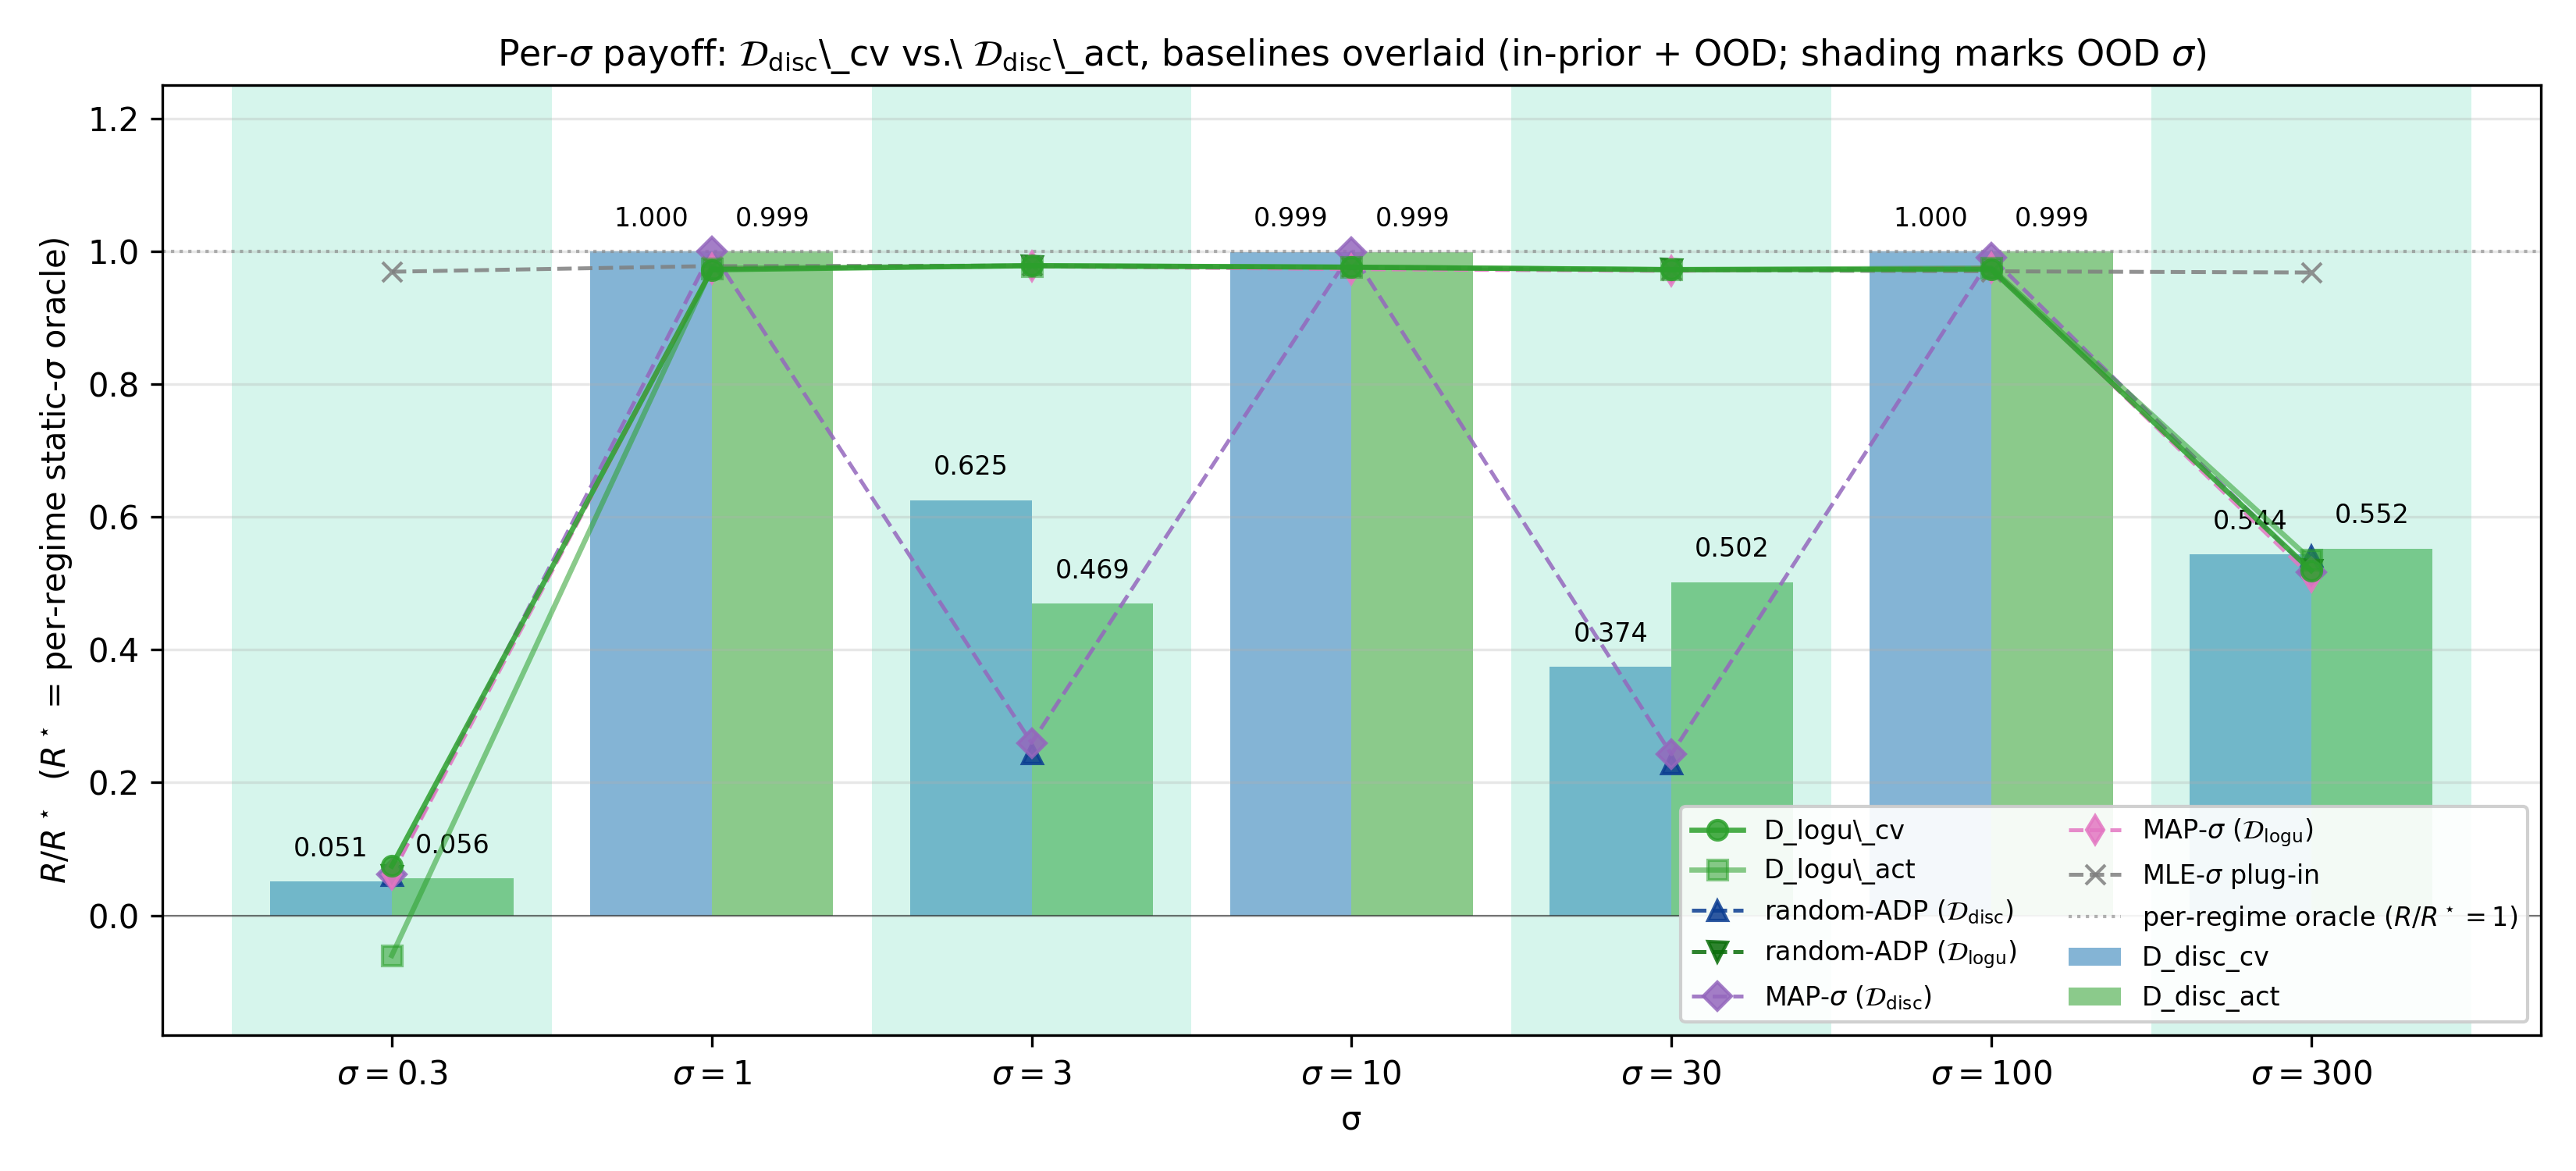
\includegraphics[width=\textwidth]{figures/per-sigma-d-disc-extended.png}
\caption{Per-$\sigma$ payoff for $\mathcal{D}_{\mathrm{disc}}$\_cv vs.\ $\mathcal{D}_{\mathrm{disc}}$\_act across all seven test $\sigma$ values, with the five data-only and prior-aware baselines overlaid as dashed lines + markers and the alternative continuous-prior models ($\mathcal{D}_{\mathrm{logu}}$\_cv, $\mathcal{D}_{\mathrm{logu}}$\_act) overlaid as solid green lines. $R^\star =$ per-regime static-$\sigma$ oracle; shading marks OOD bins.}
\label{fig:per-sigma-disc-extended}
\end{figure}

The two interpolation bins $\sigma = 3$ and $\sigma = 30$ in Figure~\ref{fig:per-sigma-disc-extended} are the clearest evidence of generalization beyond the training prior. $\mathcal{D}_{\mathrm{disc}}$\_cv was trained on a prior supported only on $\sigma \in \{1, 10, 100\}$, yet at both $\sigma = 3$ and $\sigma = 30$ its competitive-ratio bars sit well above the matched random-ADP-disc oracle --- which is Bayes-optimal under that same three-point prior and therefore collapses toward its nearest training mode (the dashed line drops to $\approx 0.24$ at $\sigma = 3$ and $\approx 0.23$ at $\sigma = 30$) --- and above the matched MAP-$\sigma$ plug-in. The $\mathcal{D}_{\mathrm{logu}}$ lines overlaid in the same panel show that an in-prior model reaches $R/R^\star \approx 0.98$ at both bins, marking the achievable ceiling without the per-regime oracle's privileged knowledge of $\sigma$. $\mathcal{D}_{\mathrm{disc}}$\_cv does not reach that ceiling, but it has clearly learned a $\sigma$-conditional threshold rule that extends past the discrete support of its training prior, outperforming the ADP routine that supplied its supervision labels.

\begin{figure}[H]
\centering
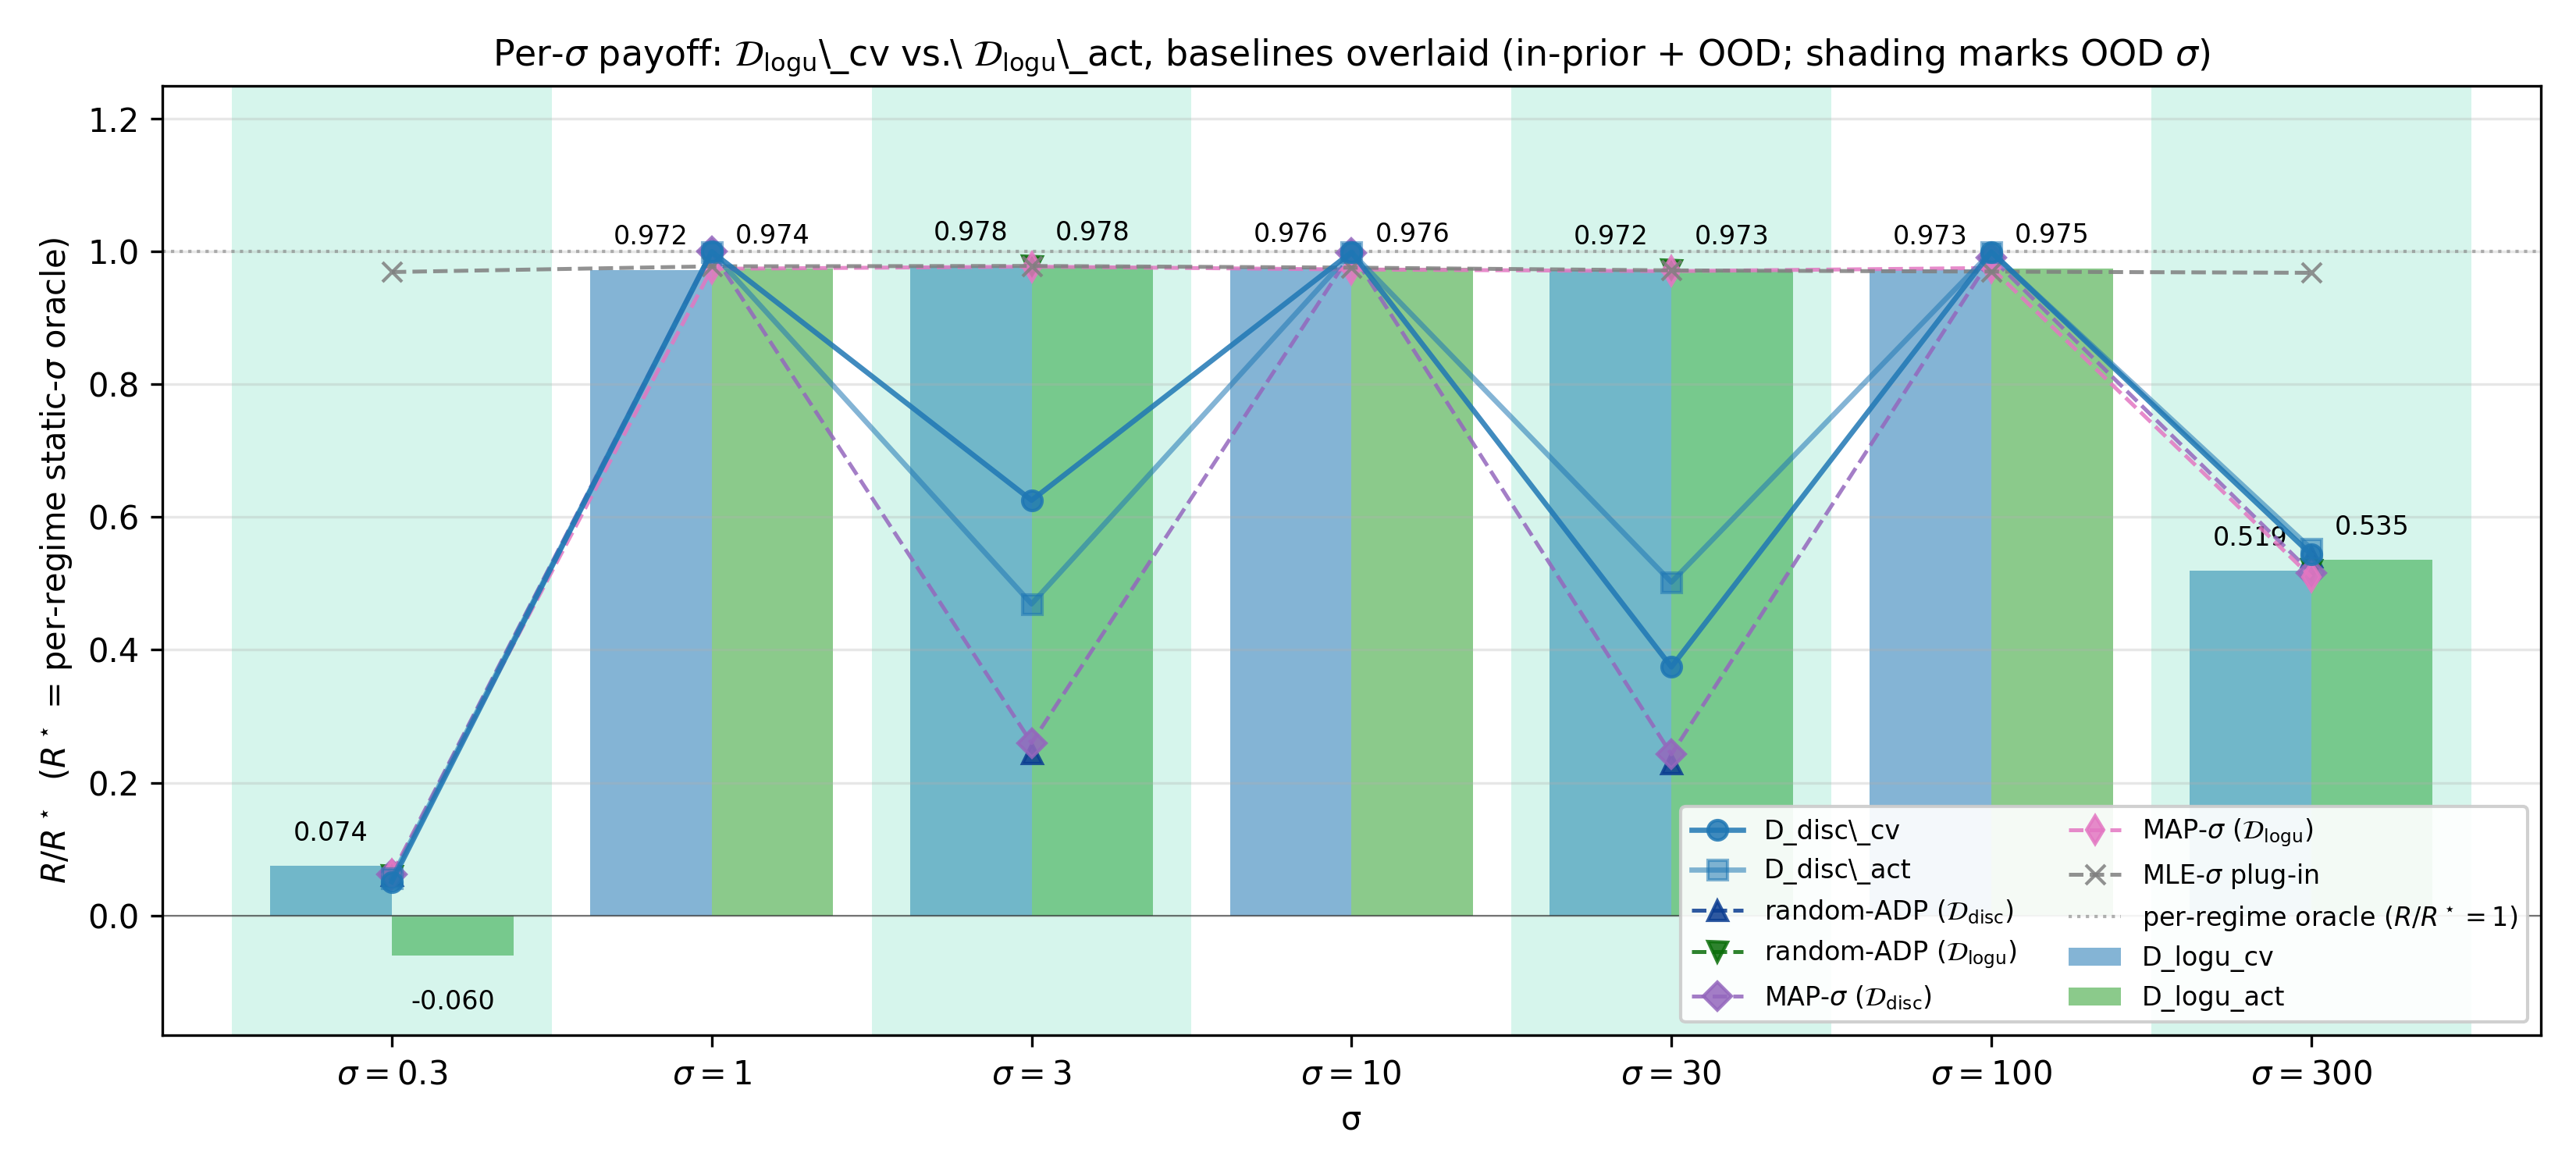
\includegraphics[width=\textwidth]{figures/per-sigma-d-logu-extended.png}
\caption{Per-$\sigma$ payoff for $\mathcal{D}_{\mathrm{logu}}$\_cv vs.\ $\mathcal{D}_{\mathrm{logu}}$\_act across all seven test $\sigma$ values, with the same five baselines and the alternative discrete-prior models ($\mathcal{D}_{\mathrm{disc}}$\_cv, $\mathcal{D}_{\mathrm{disc}}$\_act) overlaid as solid blue lines. $R^\star =$ per-regime static-$\sigma$ oracle.}
\label{fig:per-sigma-logu-extended}
\end{figure}

\begin{figure}[H]
\centering
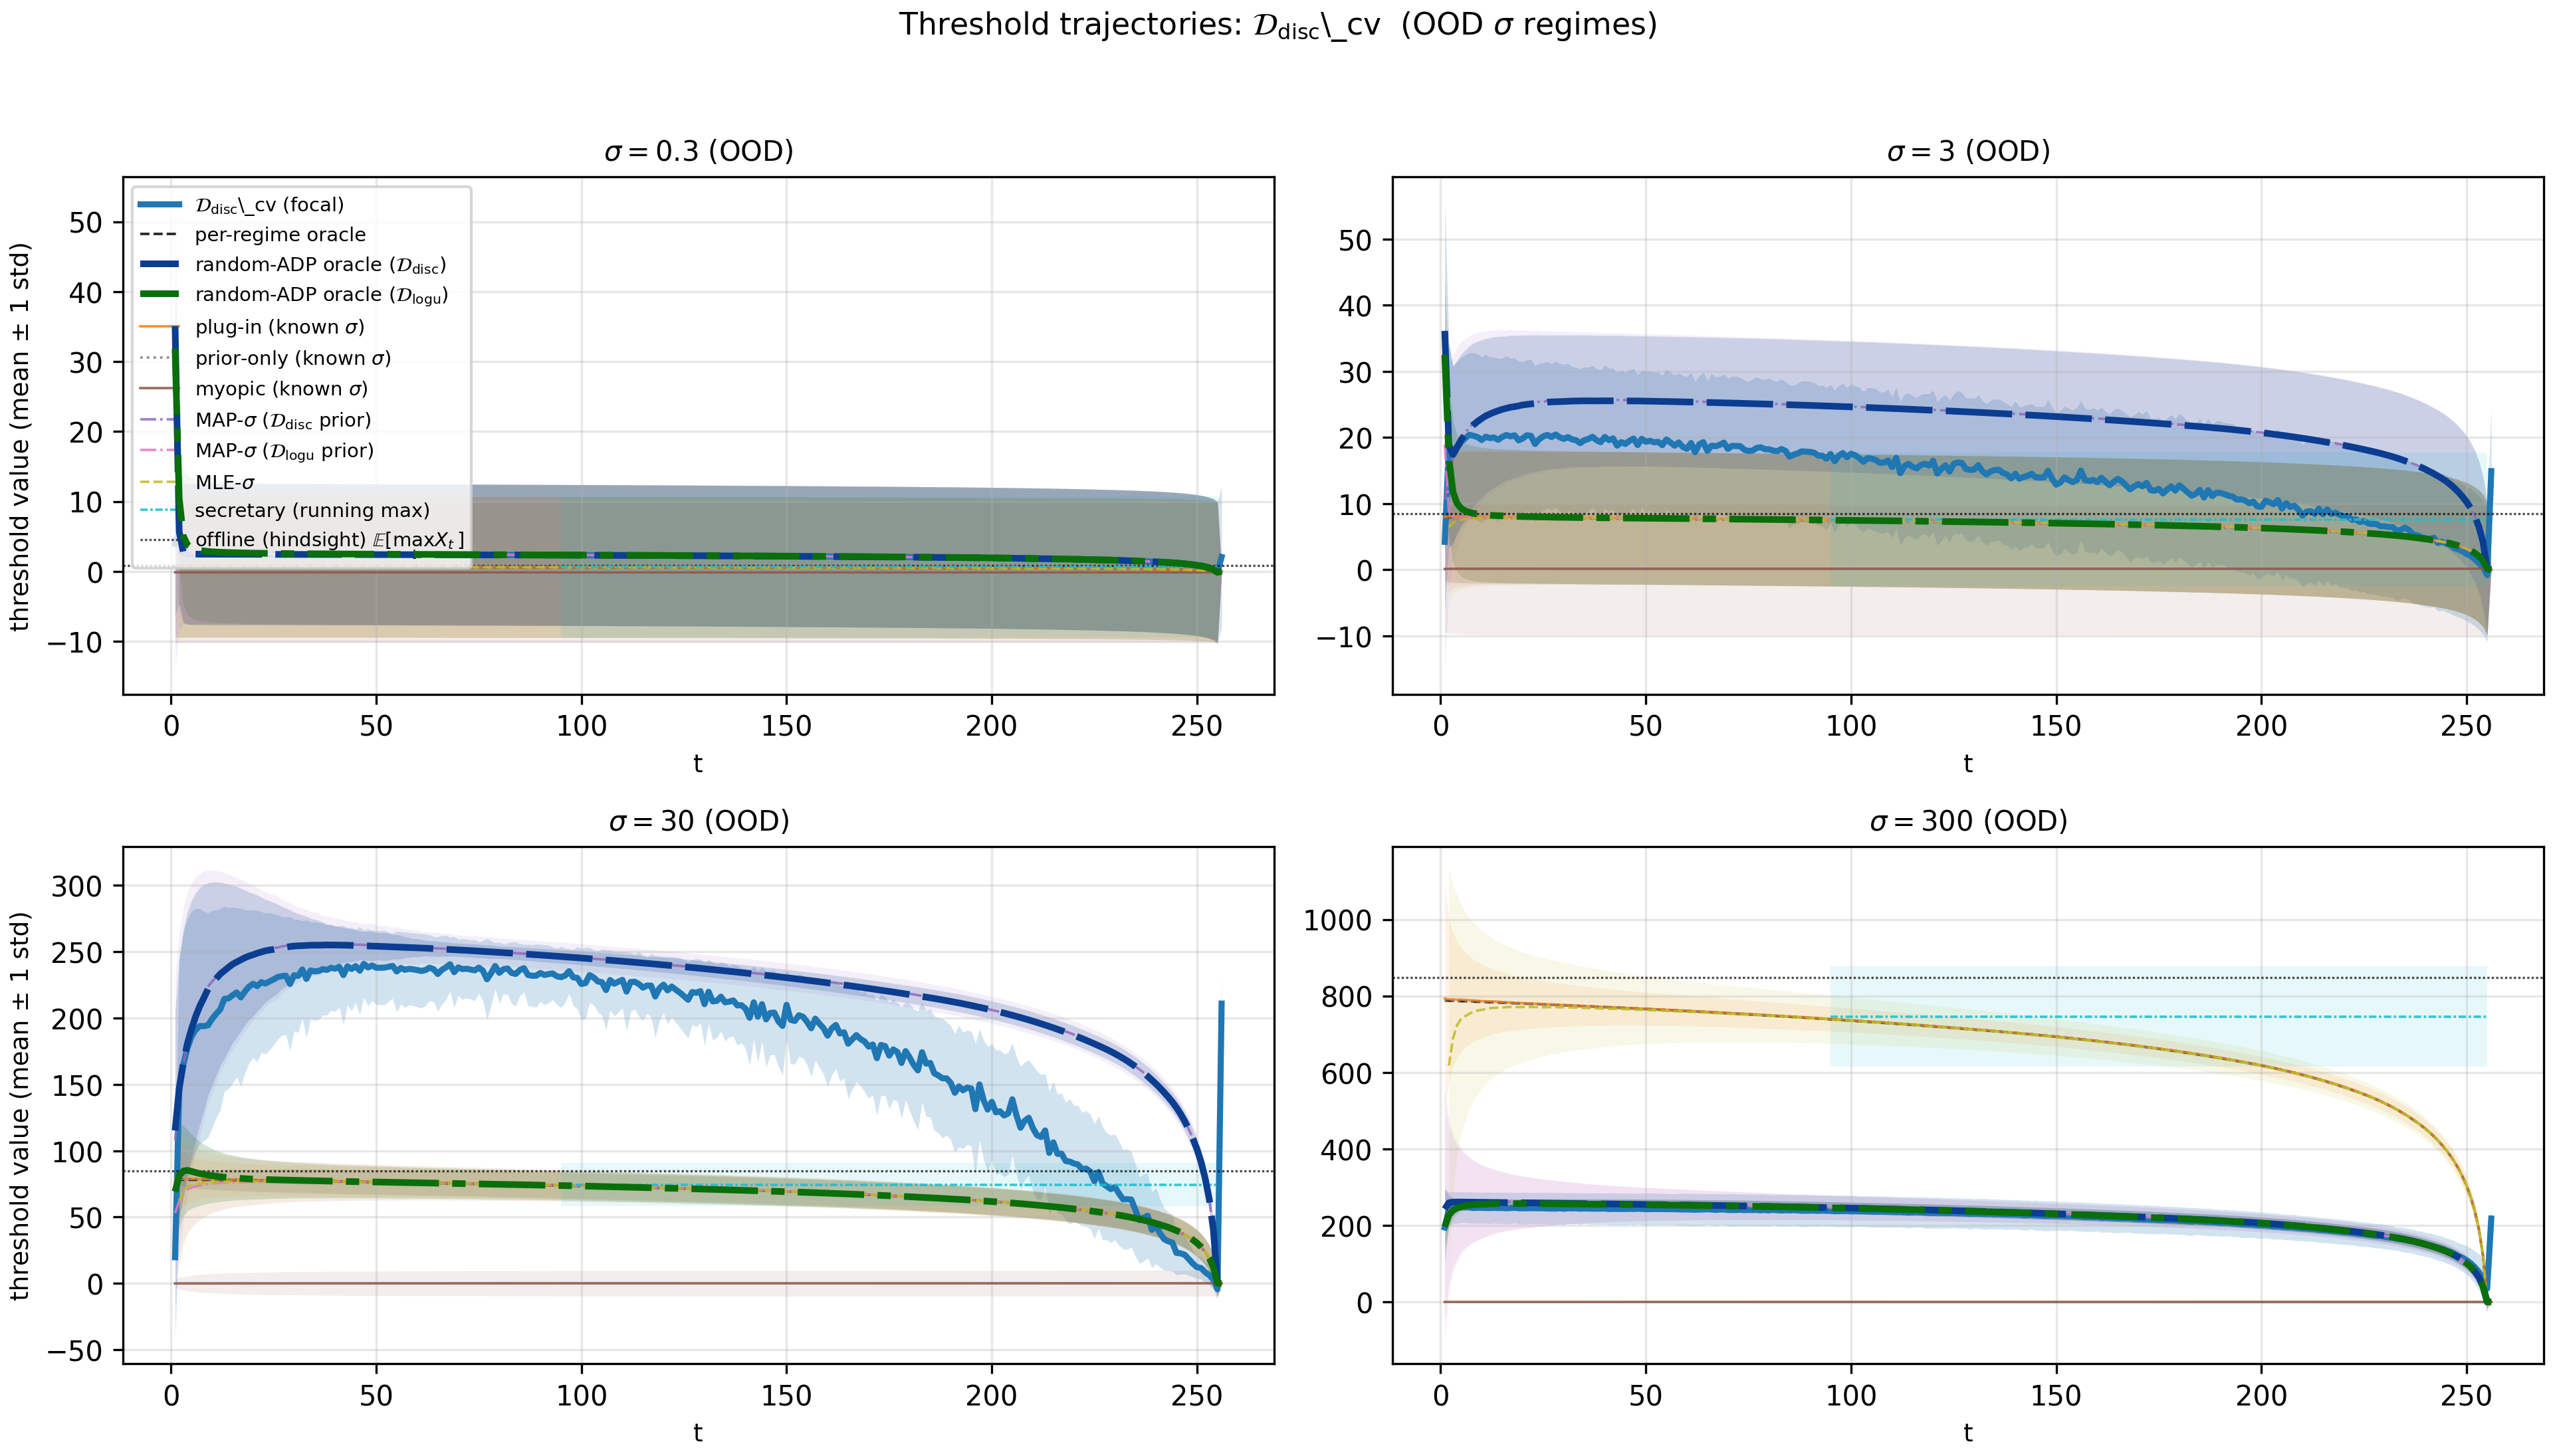
\includegraphics[width=\textwidth]{figures/trajectories-d-disc-cv-ood.png}
\caption{Threshold trajectories for $\mathcal{D}_{\mathrm{disc}}$\_cv on the four OOD test regimes ($\sigma \in \{0.3, 3, 30, 300\}$). Each panel overlays the trained model (focal, blue) on every baseline from Section~\ref{sec:baselines}, with the random-ADP oracles emphasised as thick long-dash lines. In-distribution panels for $\sigma \in \{1, 10, 100\}$ are reported separately (Figure~\ref{fig:traj-disc-cv}).}
\label{fig:traj-disc-cv-ood}
\end{figure}

Figure~\ref{fig:traj-disc-cv-ood} confirms the same story at the trajectory level. In both the $\sigma = 3$ (top-right) and $\sigma = 30$ (bottom-left) panels, $\mathcal{D}_{\mathrm{disc}}$\_cv's threshold settles at an interpolated level between its two nearest training $\sigma$ values, well above the random-ADP-disc oracle (which collapses to its nearest training mode) and above the matched MAP-$\sigma$ plug-in. The trained model does not reach the per-regime static-$\sigma$ oracle (black dashed) --- that oracle knows the true $\sigma$ exactly --- but the gap pattern is uniform across both interpolation bins and matches the competitive-ratio gaps in Figure~\ref{fig:per-sigma-disc-extended}, so the bars and the trajectories tell the same story by two different routes.

\begin{figure}[H]
\centering
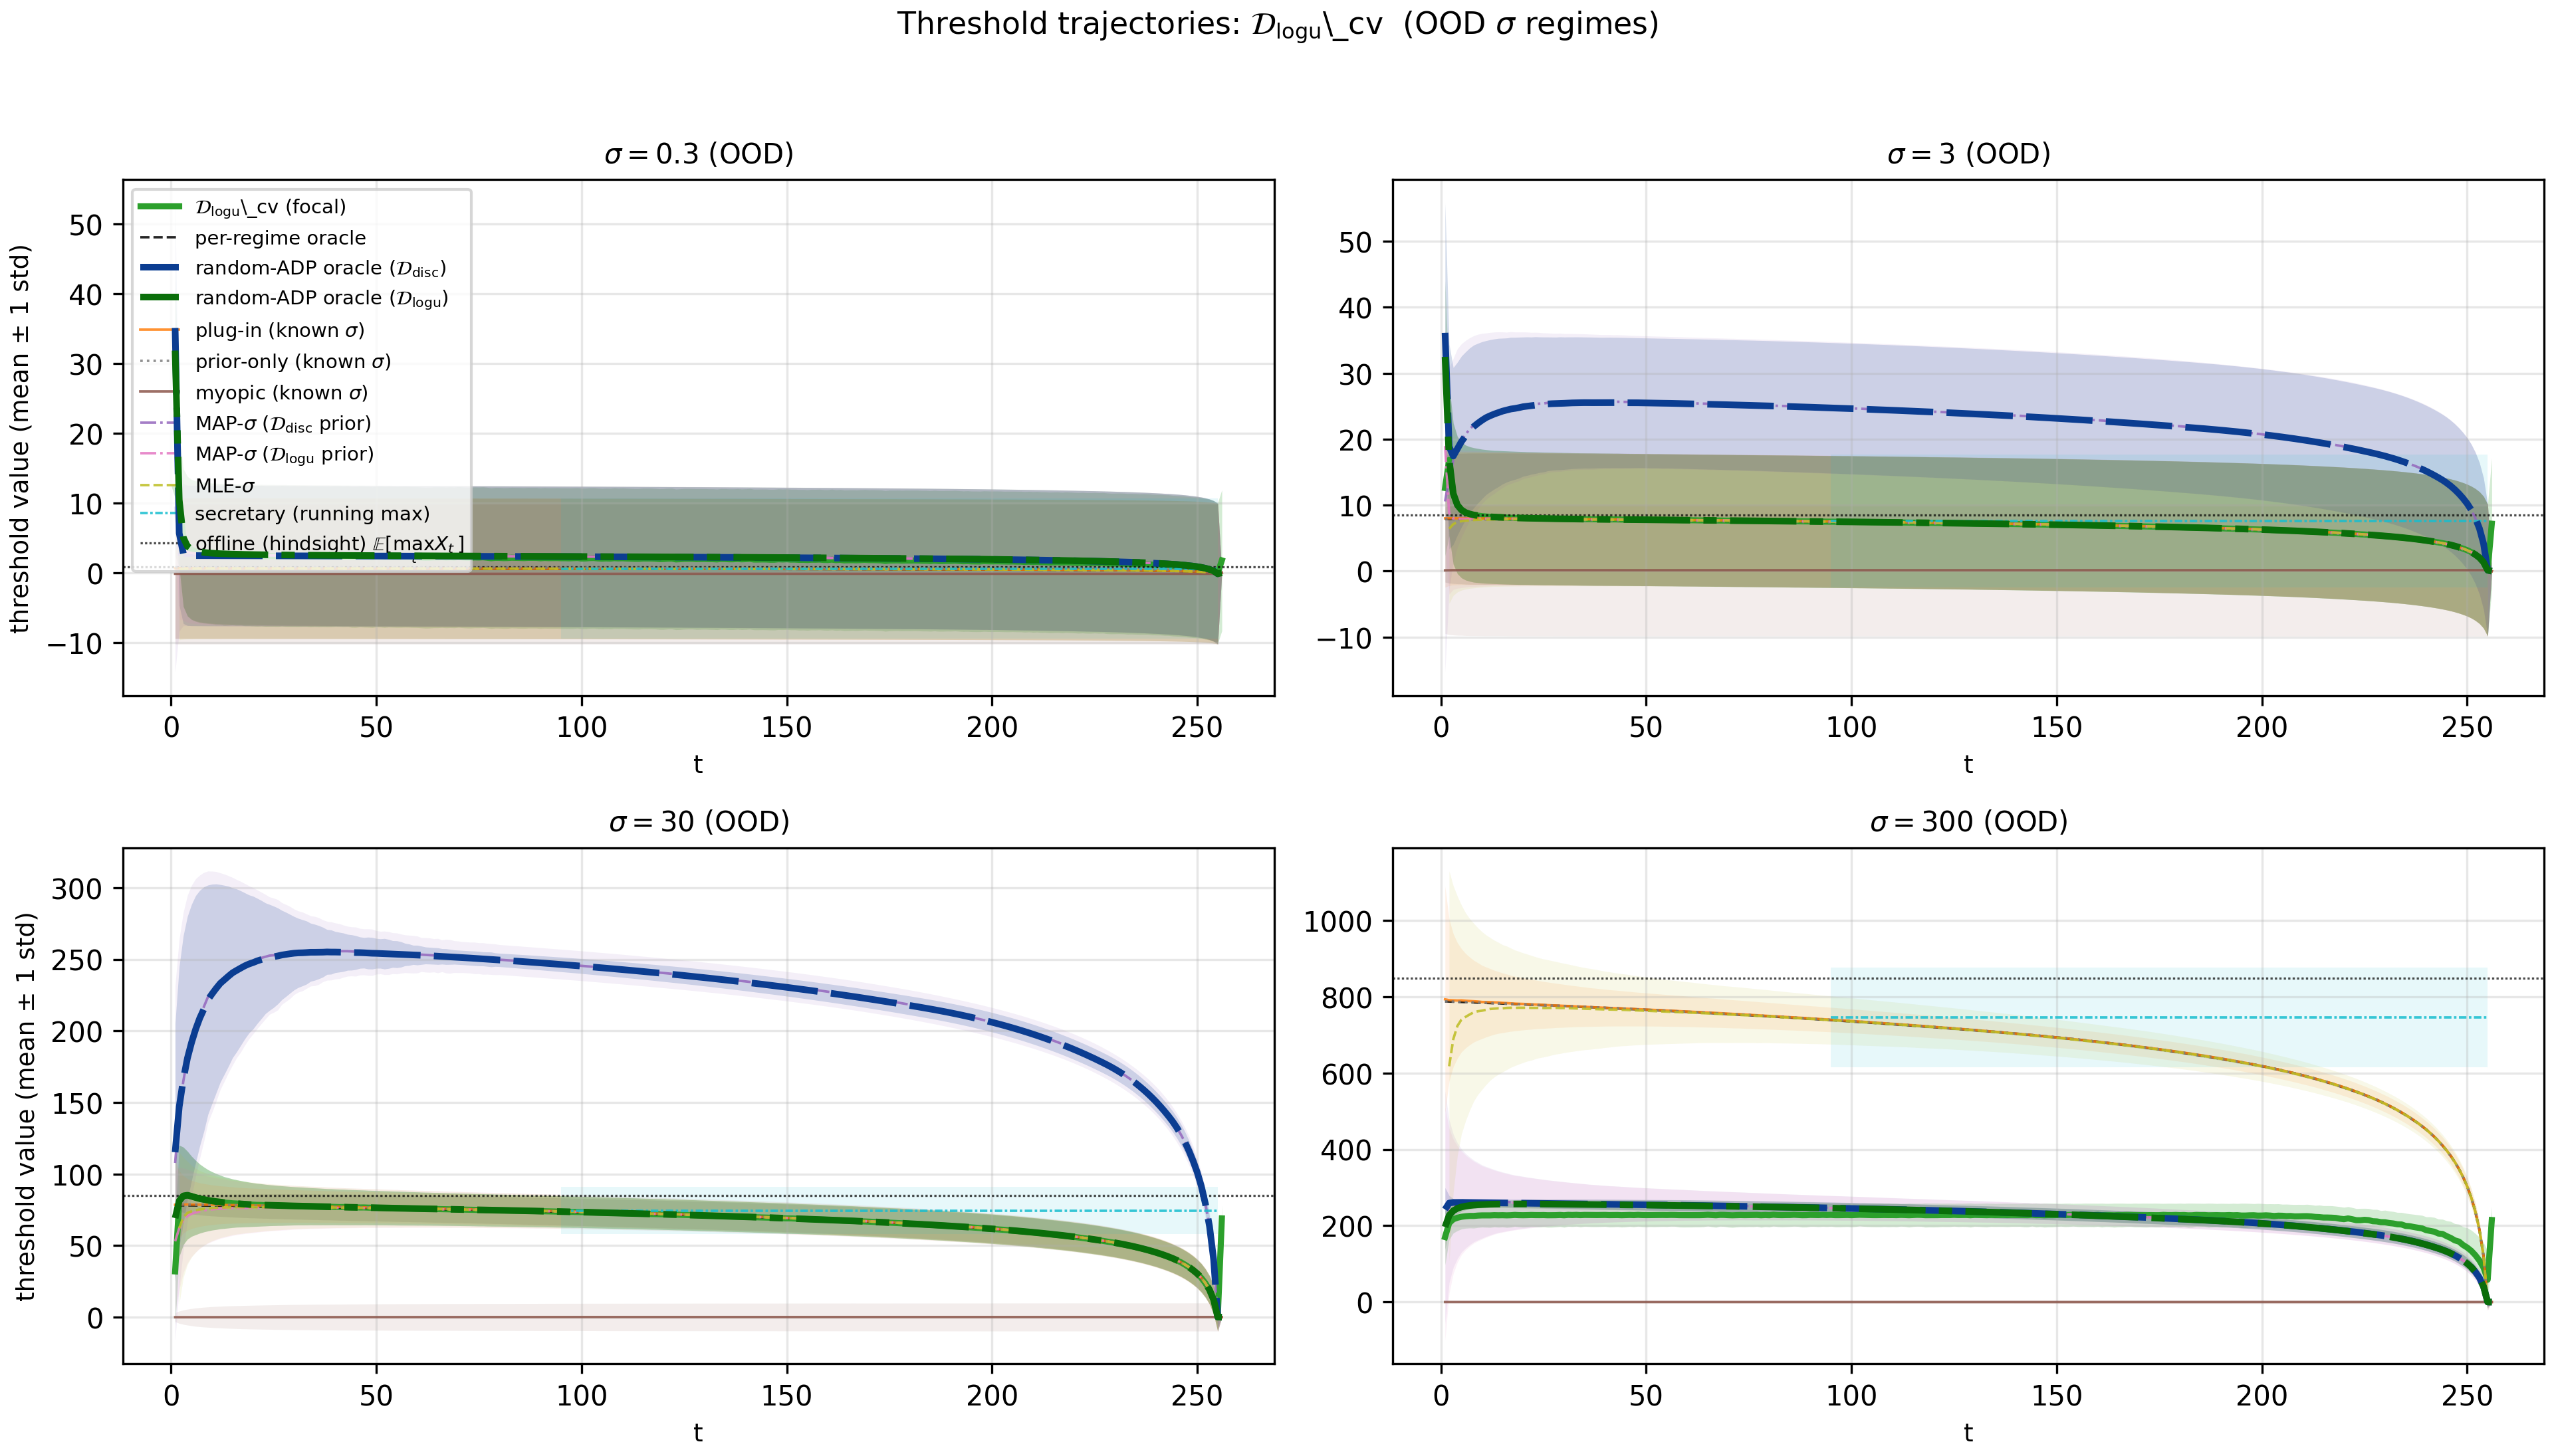
\includegraphics[width=\textwidth]{figures/trajectories-d-logu-cv-ood.png}
\caption{Threshold trajectories for $\mathcal{D}_{\mathrm{logu}}$\_cv on the four OOD test regimes.}
\label{fig:traj-logu-cv-ood}
\end{figure}

\subsection{Temporal shift}
\label{sec:res-shift}

Matching the per-regime oracle on average (Sections~\ref{sec:res-disc}--\ref{sec:res-ood}) does not by itself prove per-sequence adaptation: a policy that averages over the prior could also score well on i.i.d.\ test regimes. To make per-sequence adaptation directly observable, we generate caches whose noise scale switches mid-sequence: for each ordered pair $(\sigma_a, \sigma_b)$ we draw $N_{\mathrm{test}} = 10^4$ sequences with $X_t \mid \mu_i, \sigma_a \sim \mathcal{N}(\mu_i, \sigma_a^2)$ for $t \le 128$ and $X_t \mid \mu_i, \sigma_b \sim \mathcal{N}(\mu_i, \sigma_b^2)$ for $t \ge 129$, with the same $\mu_i \sim \mathcal{N}(\mu_0, \tau_0^2)$ throughout. Experiment B.1 uses pairs from the training-prior support $\{1, 10, 100\}$; Experiment B.2 uses pairs from the OOD support $\{3, 30, 300\}$.

\paragraph{Adaptation progress $\rho_t$.} The model's threshold $\widehat C_t$ should sit near the static-$\sigma_a$ oracle's threshold while $t \le 128$ and migrate toward the static-$\sigma_b$ oracle's threshold for $t > 128$. To put this on a common axis across all pairs --- thresholds span orders of magnitude as $\sigma$ ranges over $\{0.3, \ldots, 300\}$ --- we measure progress in log-units against the population-mean reference of each static-$\sigma$ oracle, i.e.\ $\langle C^\star_{\sigma_a, t}\rangle$ averaged over $N_{\mathrm{test}}$ iid-$\sigma_a$ sequences (and analogously for $\sigma_b$). The normalized adaptation ratio is
\[
\rho_t \;:=\; \frac{\log |\widehat C_t| - \log |\langle C^\star_{\sigma_a, t}\rangle|}{\log |\langle C^\star_{\sigma_b, t}\rangle| - \log |\langle C^\star_{\sigma_a, t}\rangle|}.
\]
By construction $\rho_t = 0$ when the model's threshold matches the pre-shift reference and $\rho_t = 1$ when it matches the post-shift reference, with linear interpolation in log space between the two. Values outside $[0, 1]$ mean the model is undershooting the pre-shift level or overshooting the post-shift level. Operating in log-space makes the metric scale-invariant; absolute values inside the log handle any sign of $\widehat C_t$. We report the population-mean $\rho_{200}$ as the ``settled'' adaptation level, far enough past the shift to read out steady-state behavior but before the terminal-horizon regime where the static oracles' thresholds collapse and $\rho_t$ becomes ill-conditioned.

\paragraph{Half-time $t_{1/2}$.} Per sequence, $t_{1/2}$ is the smallest $\Delta t \ge 1$ such that $\rho_{128 + \Delta t} \ge 0.5$ --- the number of post-shift observations the model needs to move halfway from the $\sigma_a$ regime to the $\sigma_b$ regime in log-threshold units. A small $t_{1/2}$ indicates fast in-context adaptation; sequences whose $\rho_t$ never reaches $0.5$ within the 128-step post-shift window are counted at the ceiling $t_{1/2} = 128$ (the ``never crossed'' column in Table~\ref{tab:res-shift-summary}). Reporting the per-sequence distribution rather than the population mean exposes within-pair heterogeneity --- some sequences happen to receive an early high-$\sigma_b$ outlier and adapt in one step, others see a long run of in-range observations that look consistent with $\sigma_a$ continuing.

The full per-shift summary statistics --- mean and $p_{10}/p_{50}/p_{90}$ percentiles of $t_{1/2}$, pre/post-shift tracking errors, and $\rho_{200}$ for each of the twenty (set, model, shift) cells --- are tabulated in Appendix~\ref{app:regime-shift-stats} (Table~\ref{tab:res-shift-summary}), together with per-sequence $t_{1/2}$ histograms (Figures~\ref{fig:t-half-hist-disc}, \ref{fig:t-half-hist-b2-disc}).

\begin{figure}[H]
\centering
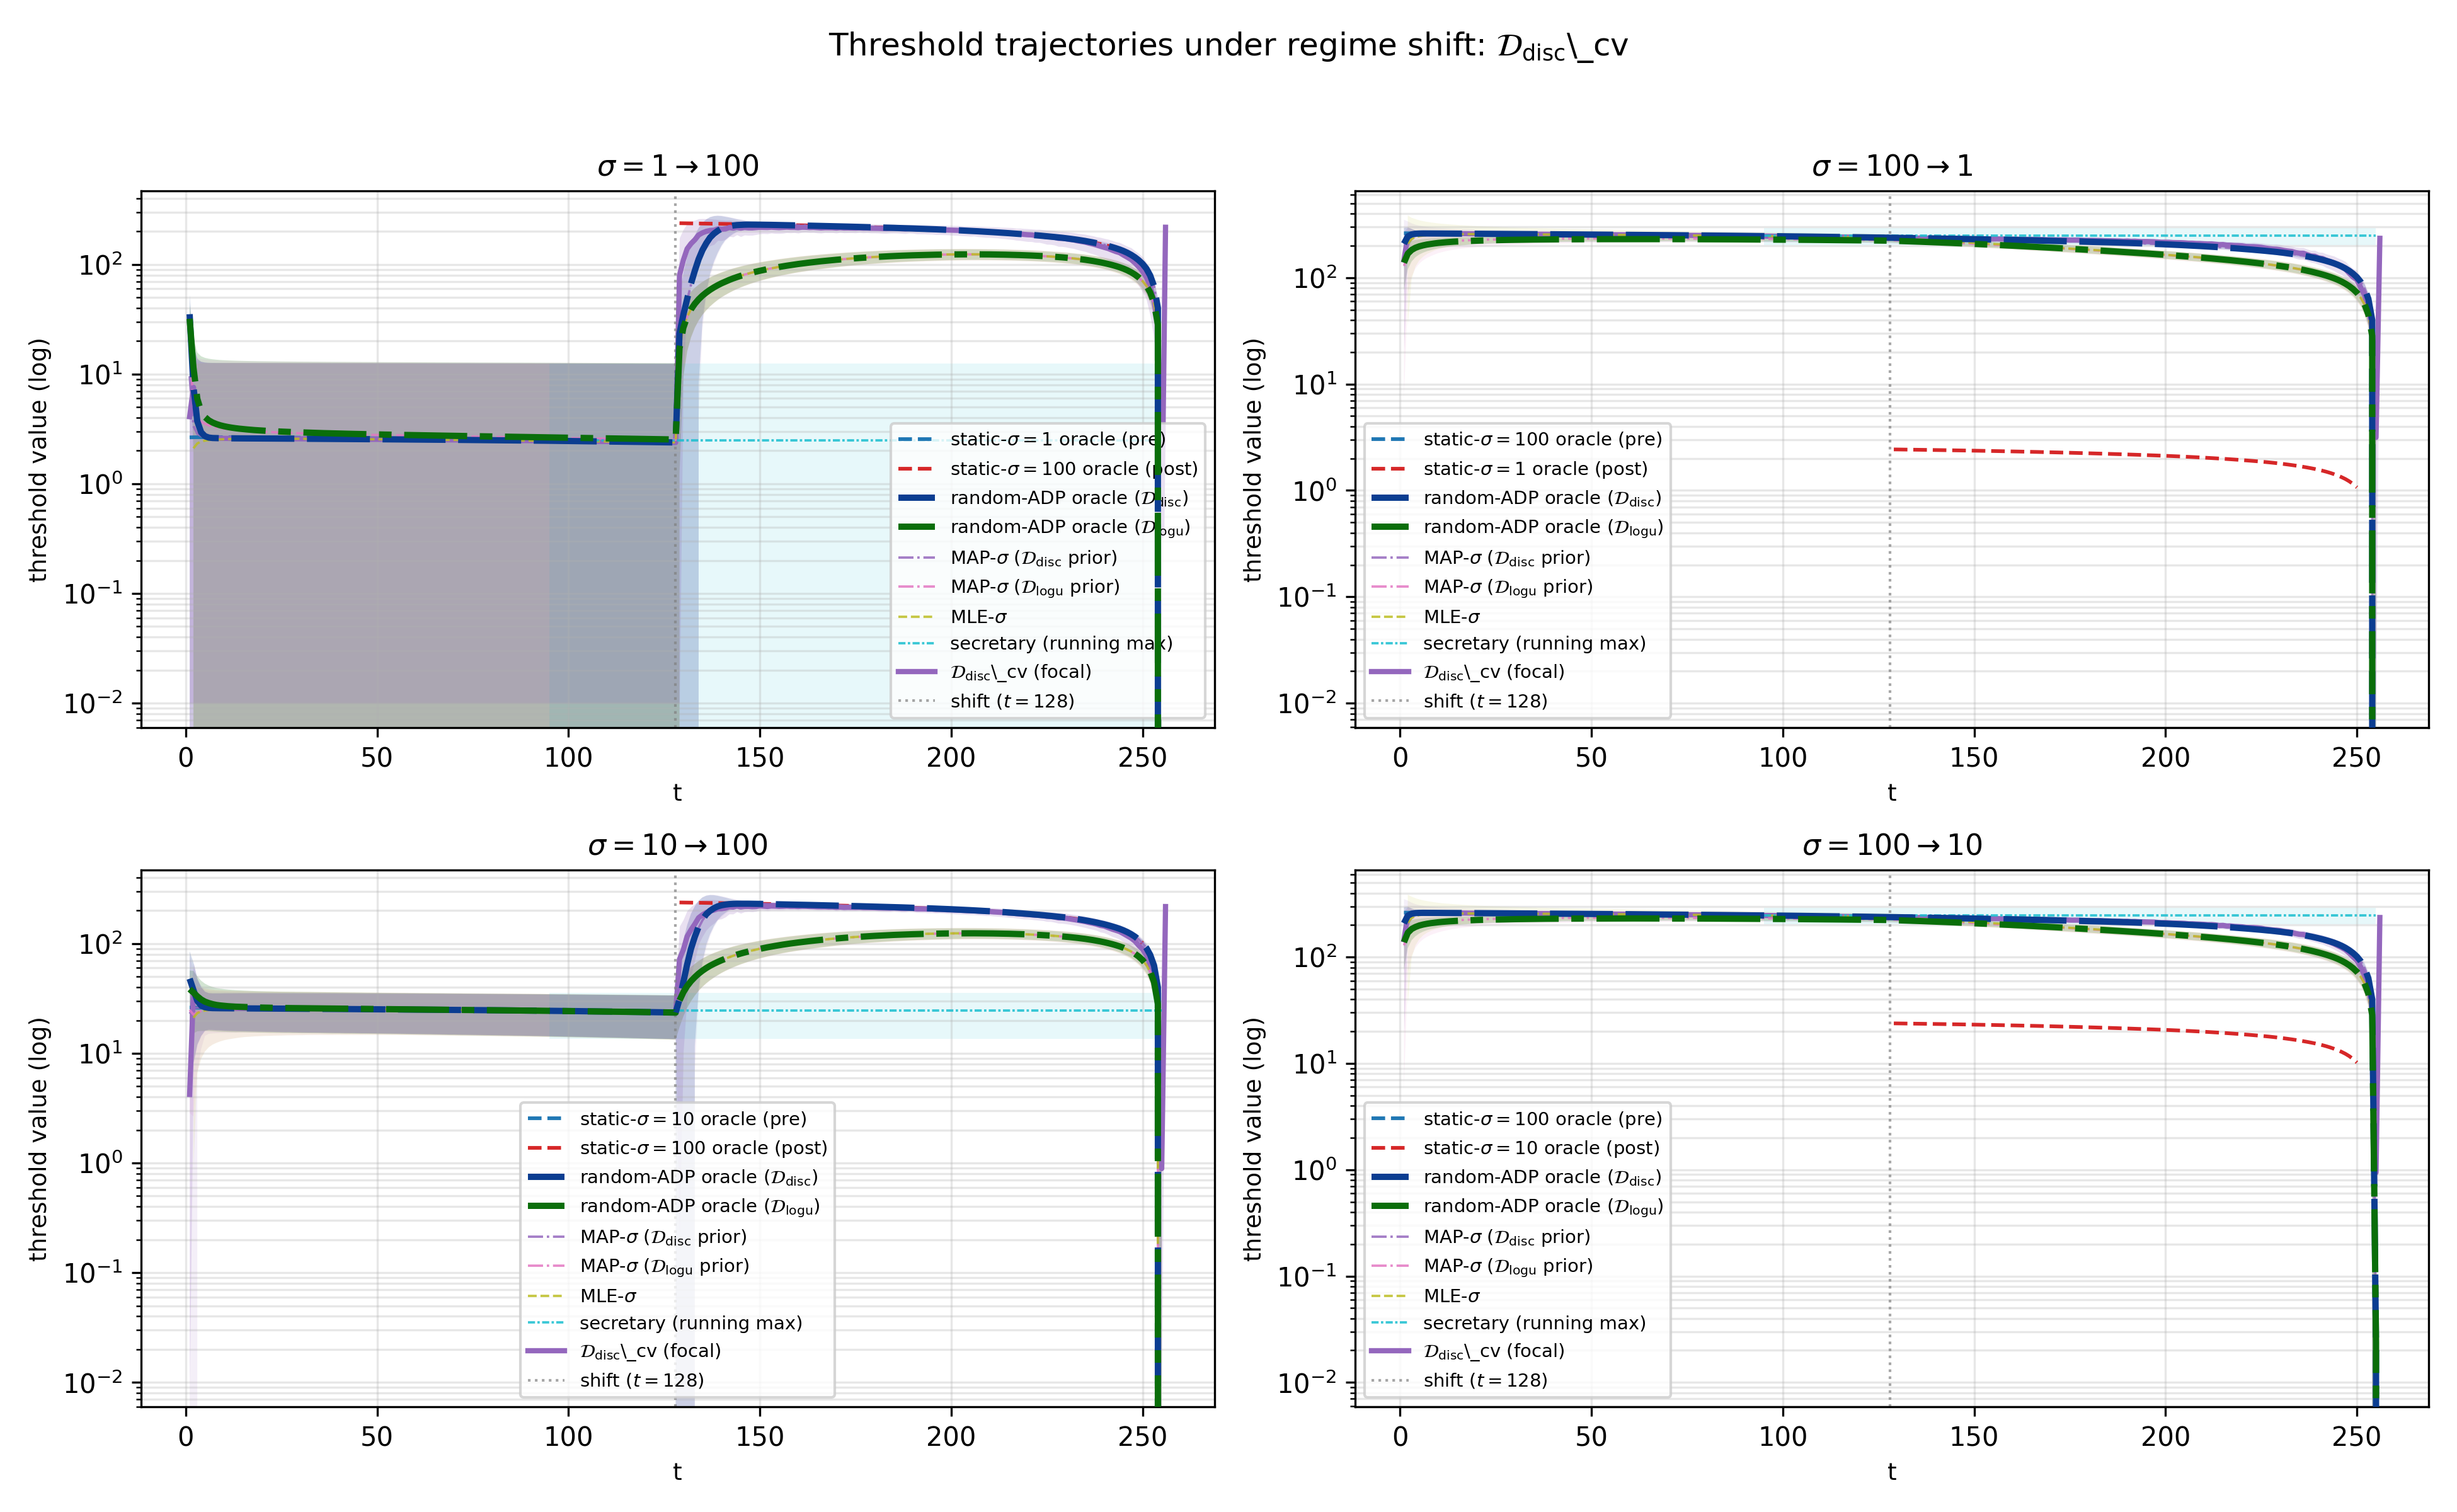
\includegraphics[width=\textwidth]{figures/trajectories-shift-D_disc_cv.png}
\caption{B.1 threshold trajectories (mean $\pm 1$ std) for $\mathcal{D}_{\mathrm{disc}}$\_cv across the four training-prior pairs. Vertical dashed line at the regime switch $t = 128$. Random-ADP oracles at the matching priors are emphasised (thick long-dash for disc, thick long-dash-dot for logu).}
\label{fig:traj-shift-disc-cv}
\end{figure}

\begin{figure}[H]
\centering
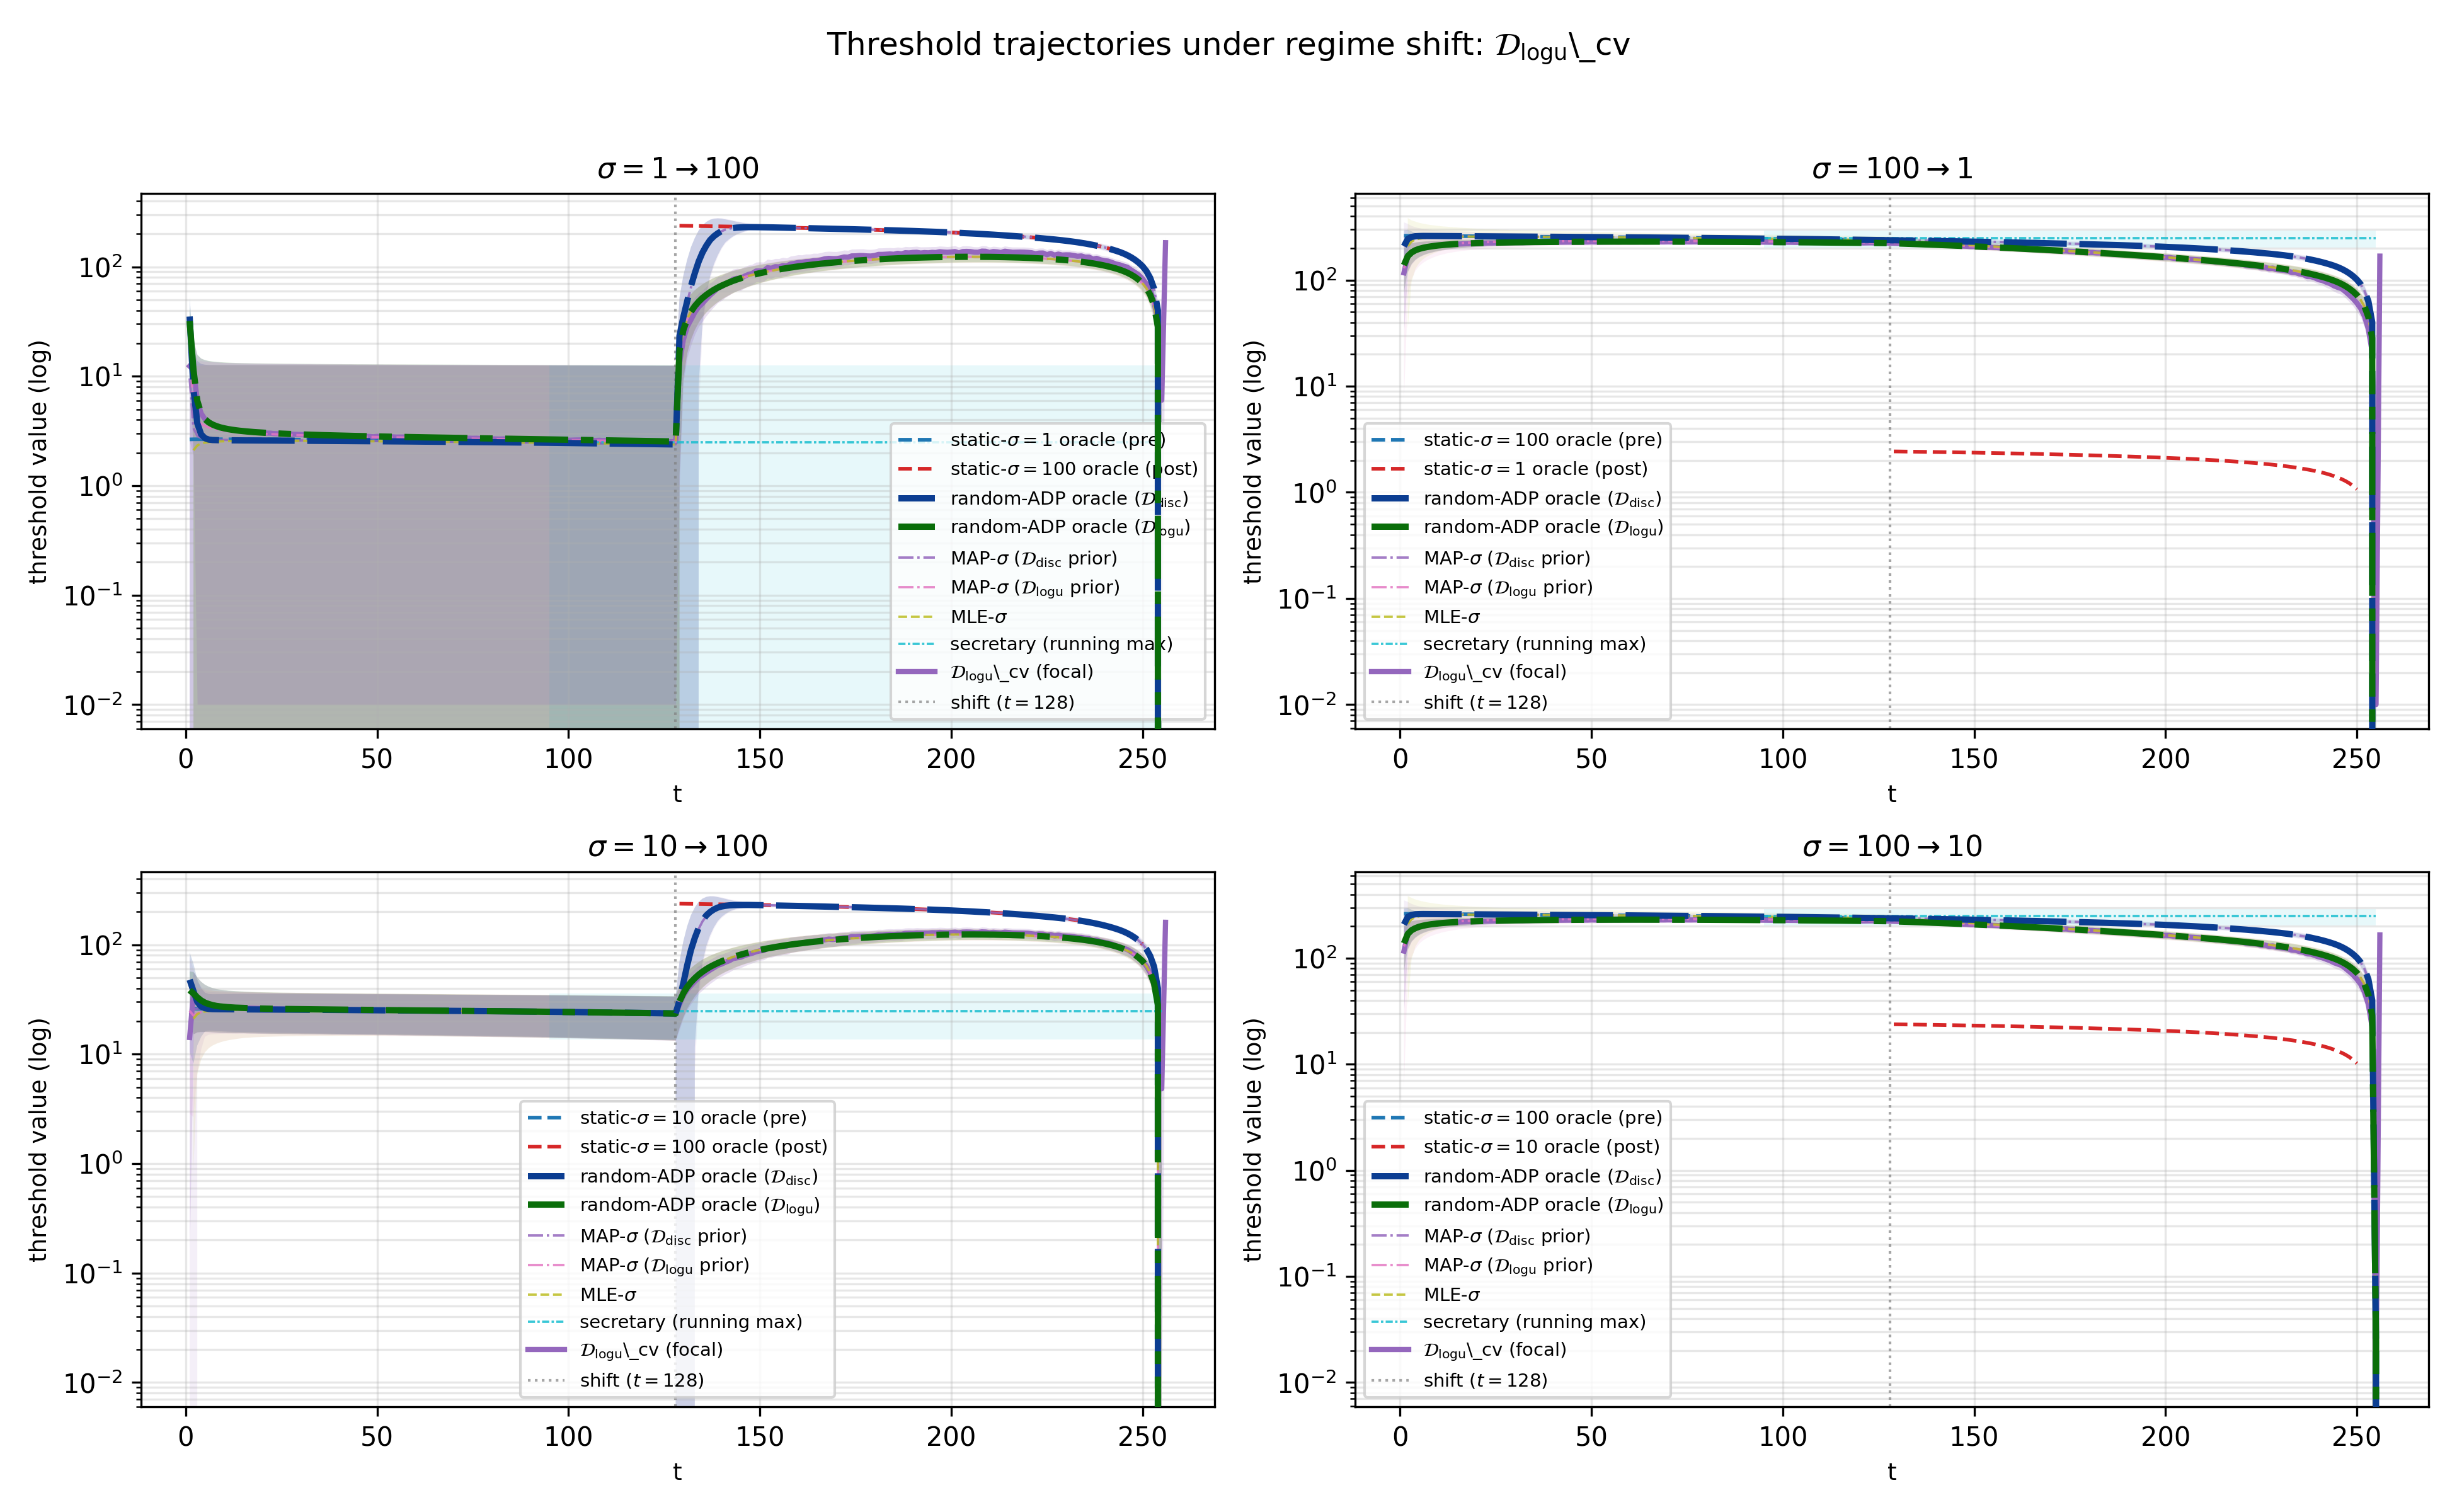
\includegraphics[width=\textwidth]{figures/trajectories-shift-D_logu_cv.png}
\caption{B.1 threshold trajectories for $\mathcal{D}_{\mathrm{logu}}$\_cv across the four training-prior pairs.}
\label{fig:traj-shift-logu-cv}
\end{figure}

\begin{figure}[H]
\centering
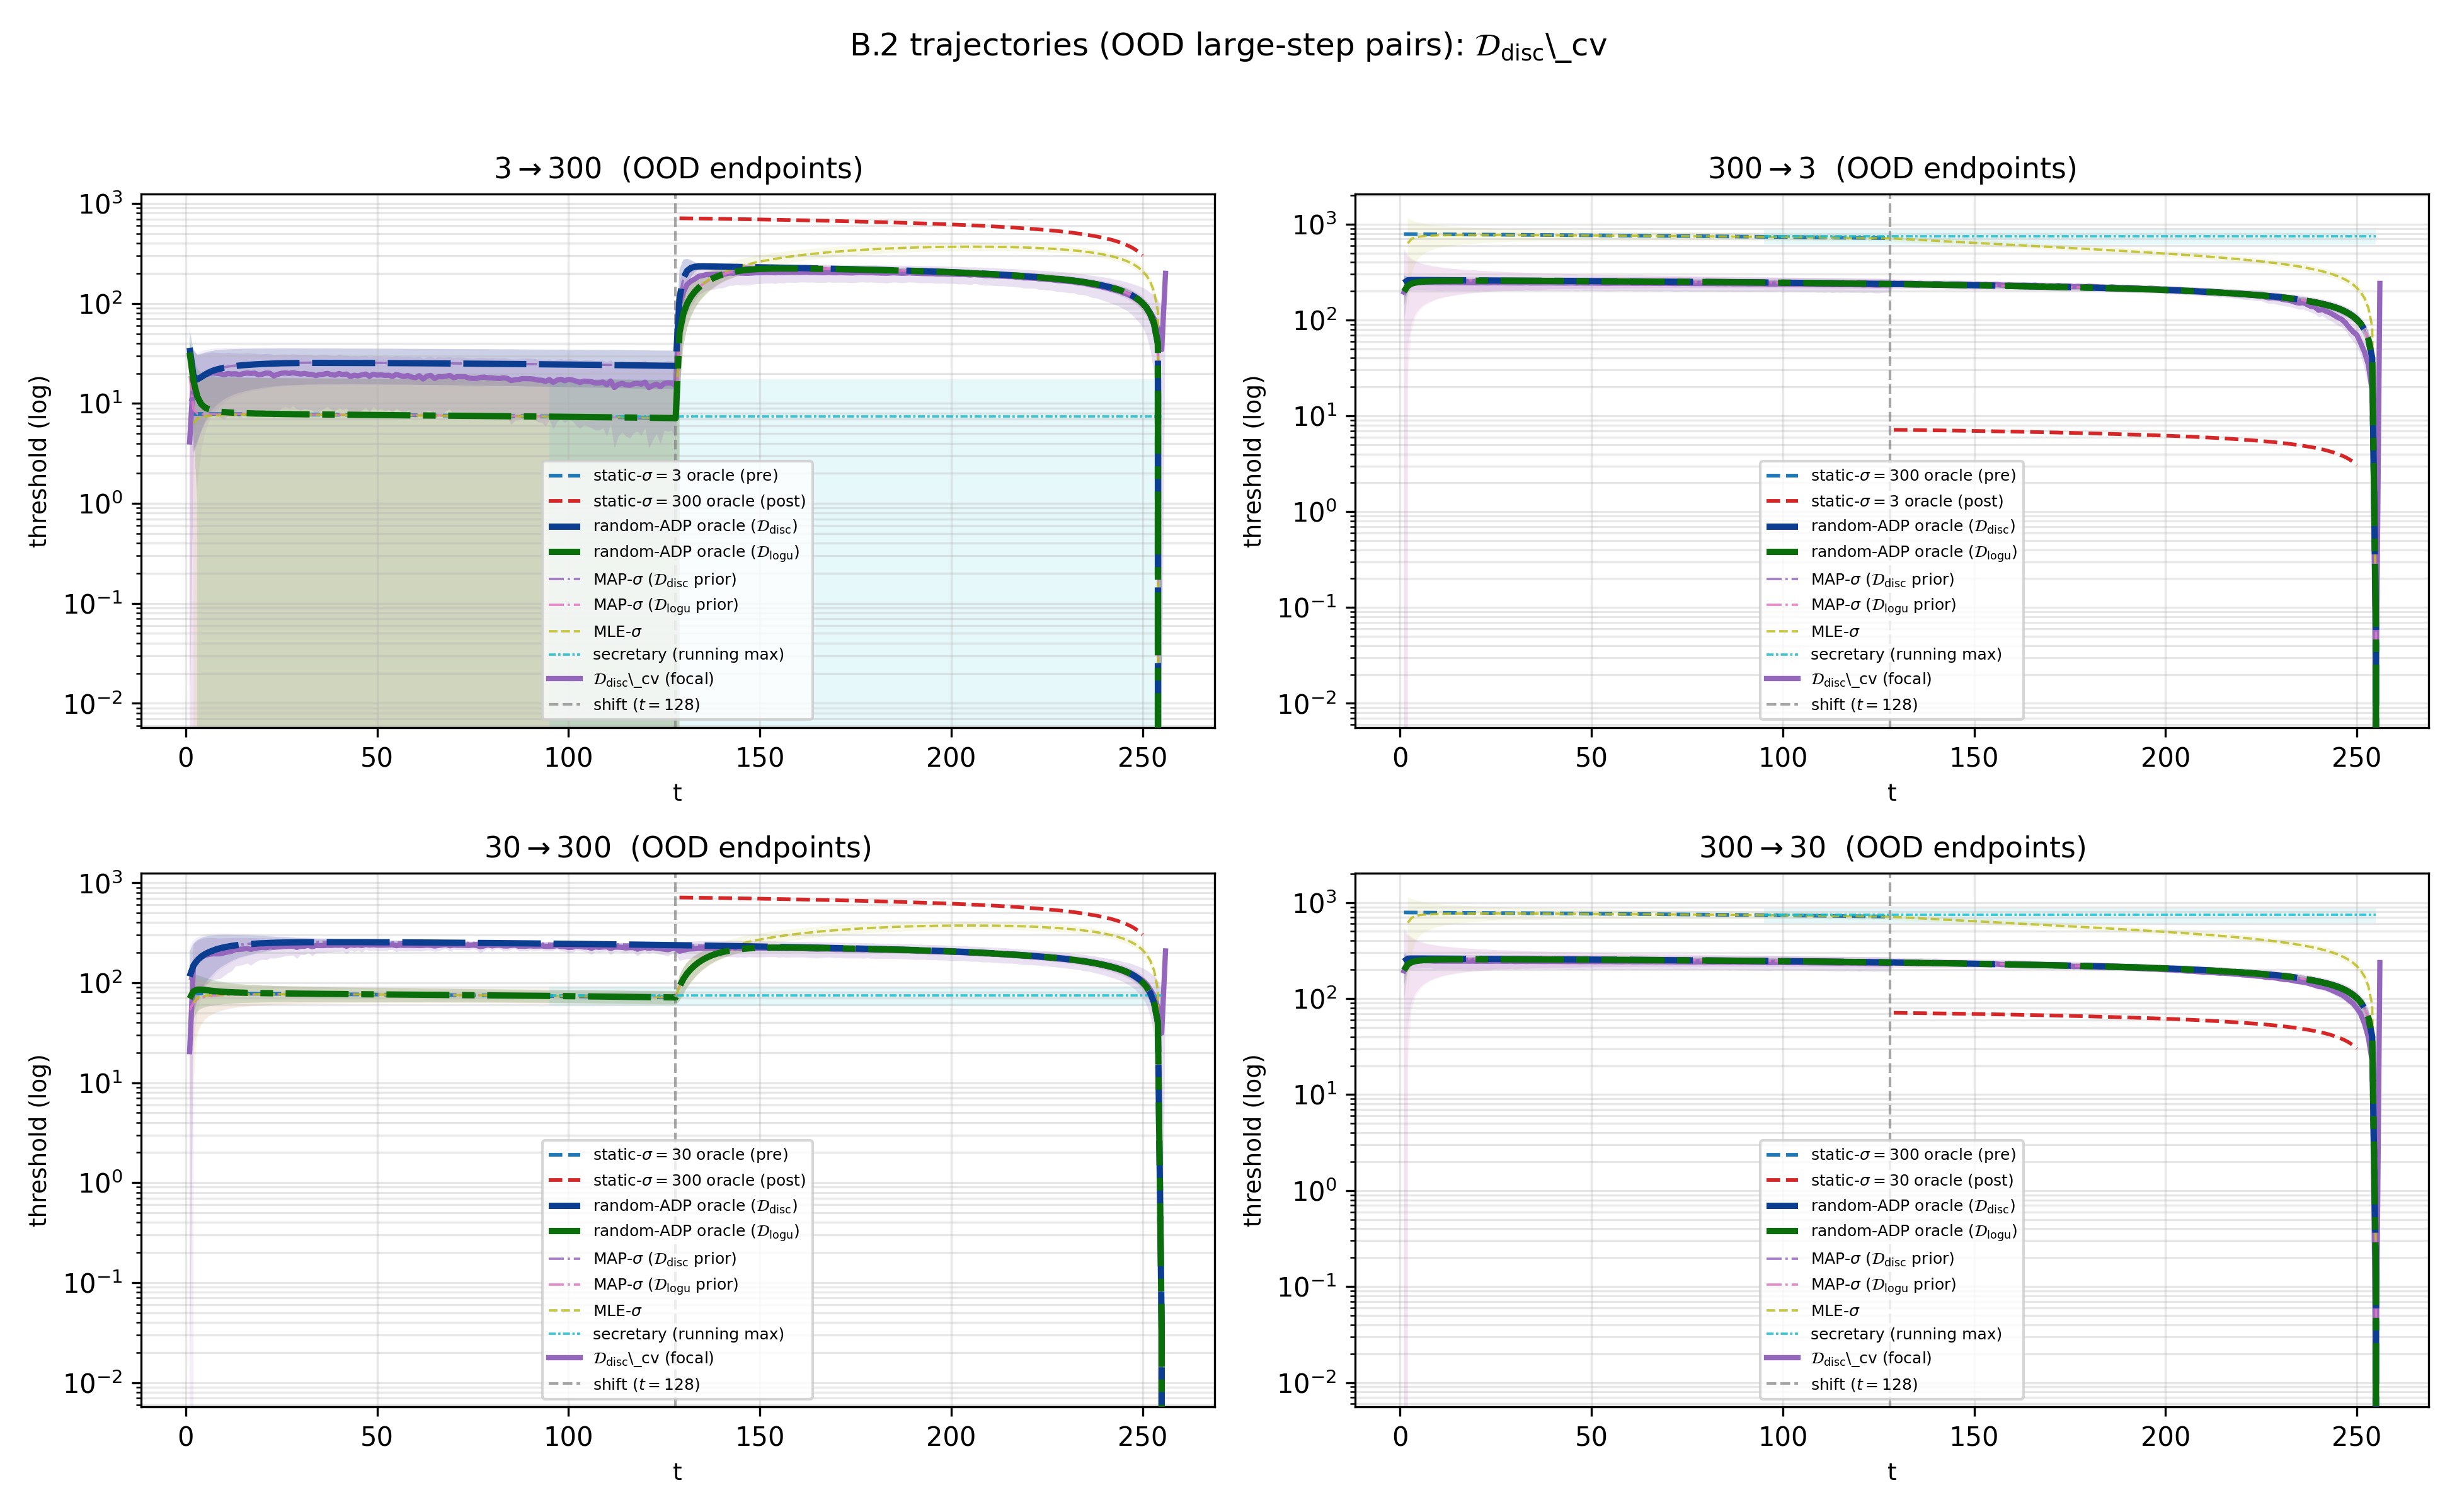
\includegraphics[width=\textwidth]{figures/trajectories-shift-b2-D_disc_cv.png}
\caption{B.2 threshold trajectories for $\mathcal{D}_{\mathrm{disc}}$\_cv across the four large-step OOD pairs.}
\label{fig:traj-shift-b2-disc-cv}
\end{figure}

\begin{figure}[H]
\centering
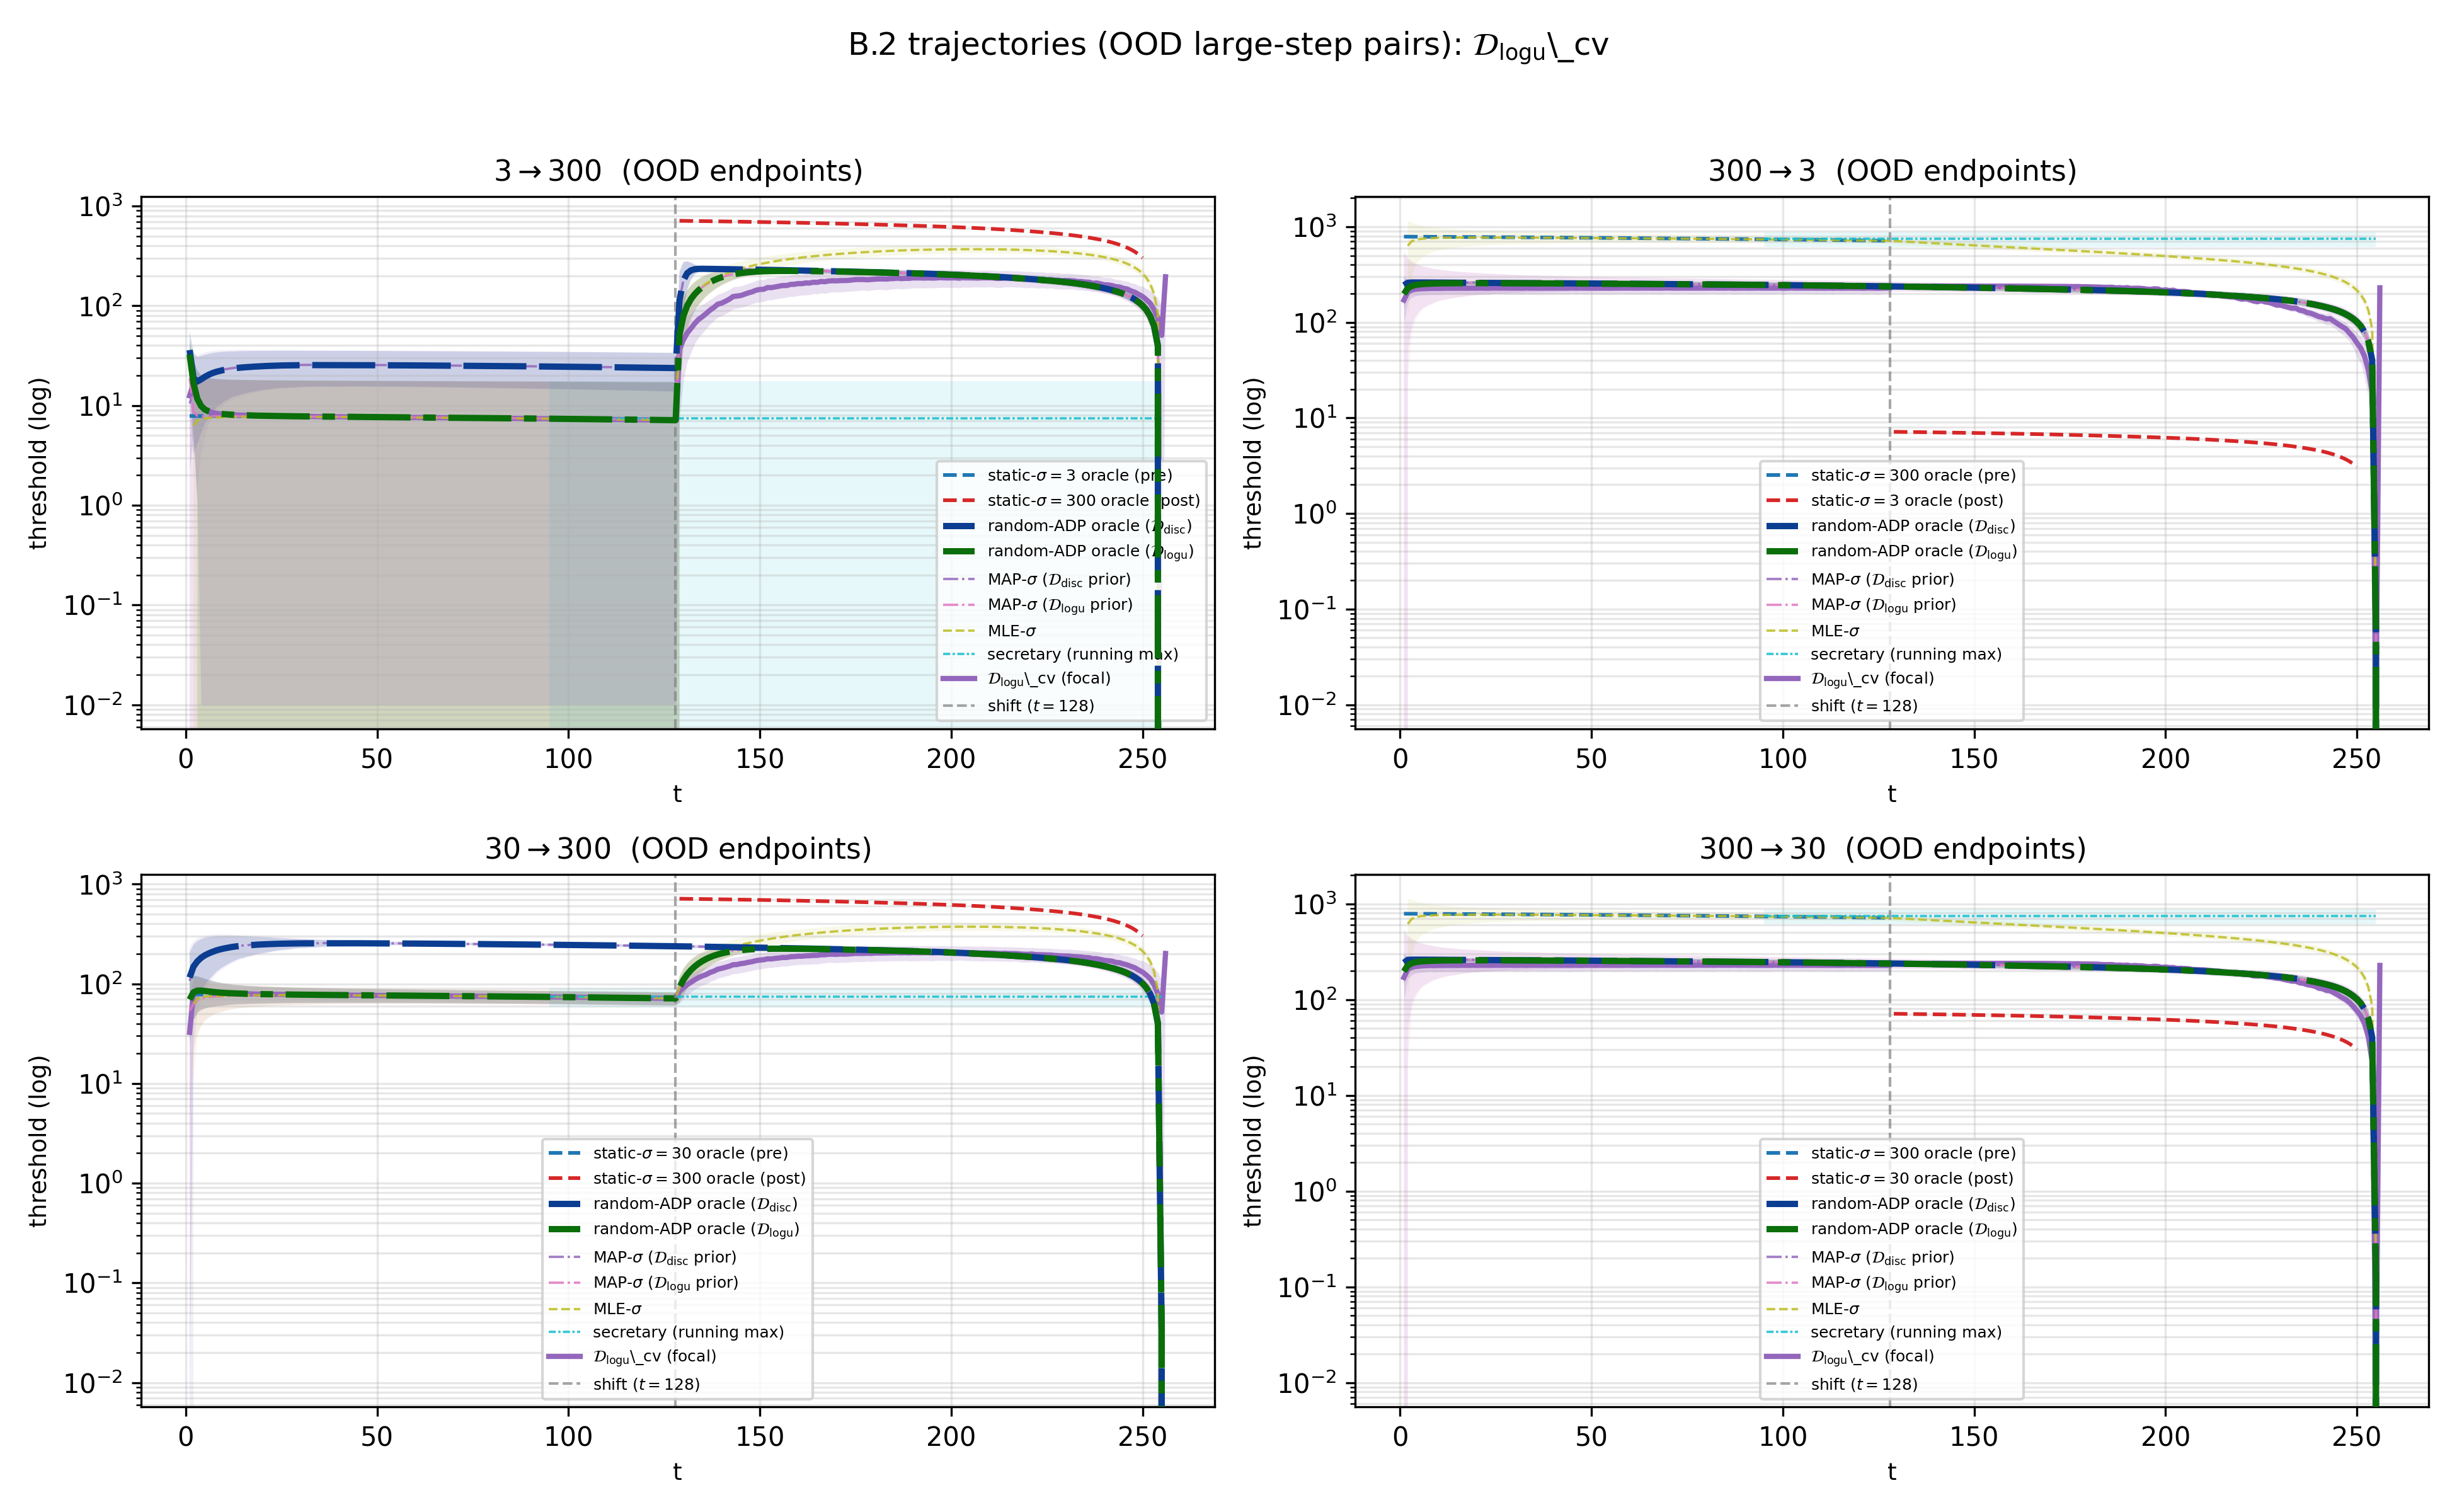
\includegraphics[width=\textwidth]{figures/trajectories-shift-b2-D_logu_cv.png}
\caption{B.2 threshold trajectories for $\mathcal{D}_{\mathrm{logu}}$\_cv across the four large-step OOD pairs.}
\label{fig:traj-shift-b2-logu-cv}
\end{figure}

\begin{figure}[H]
\centering
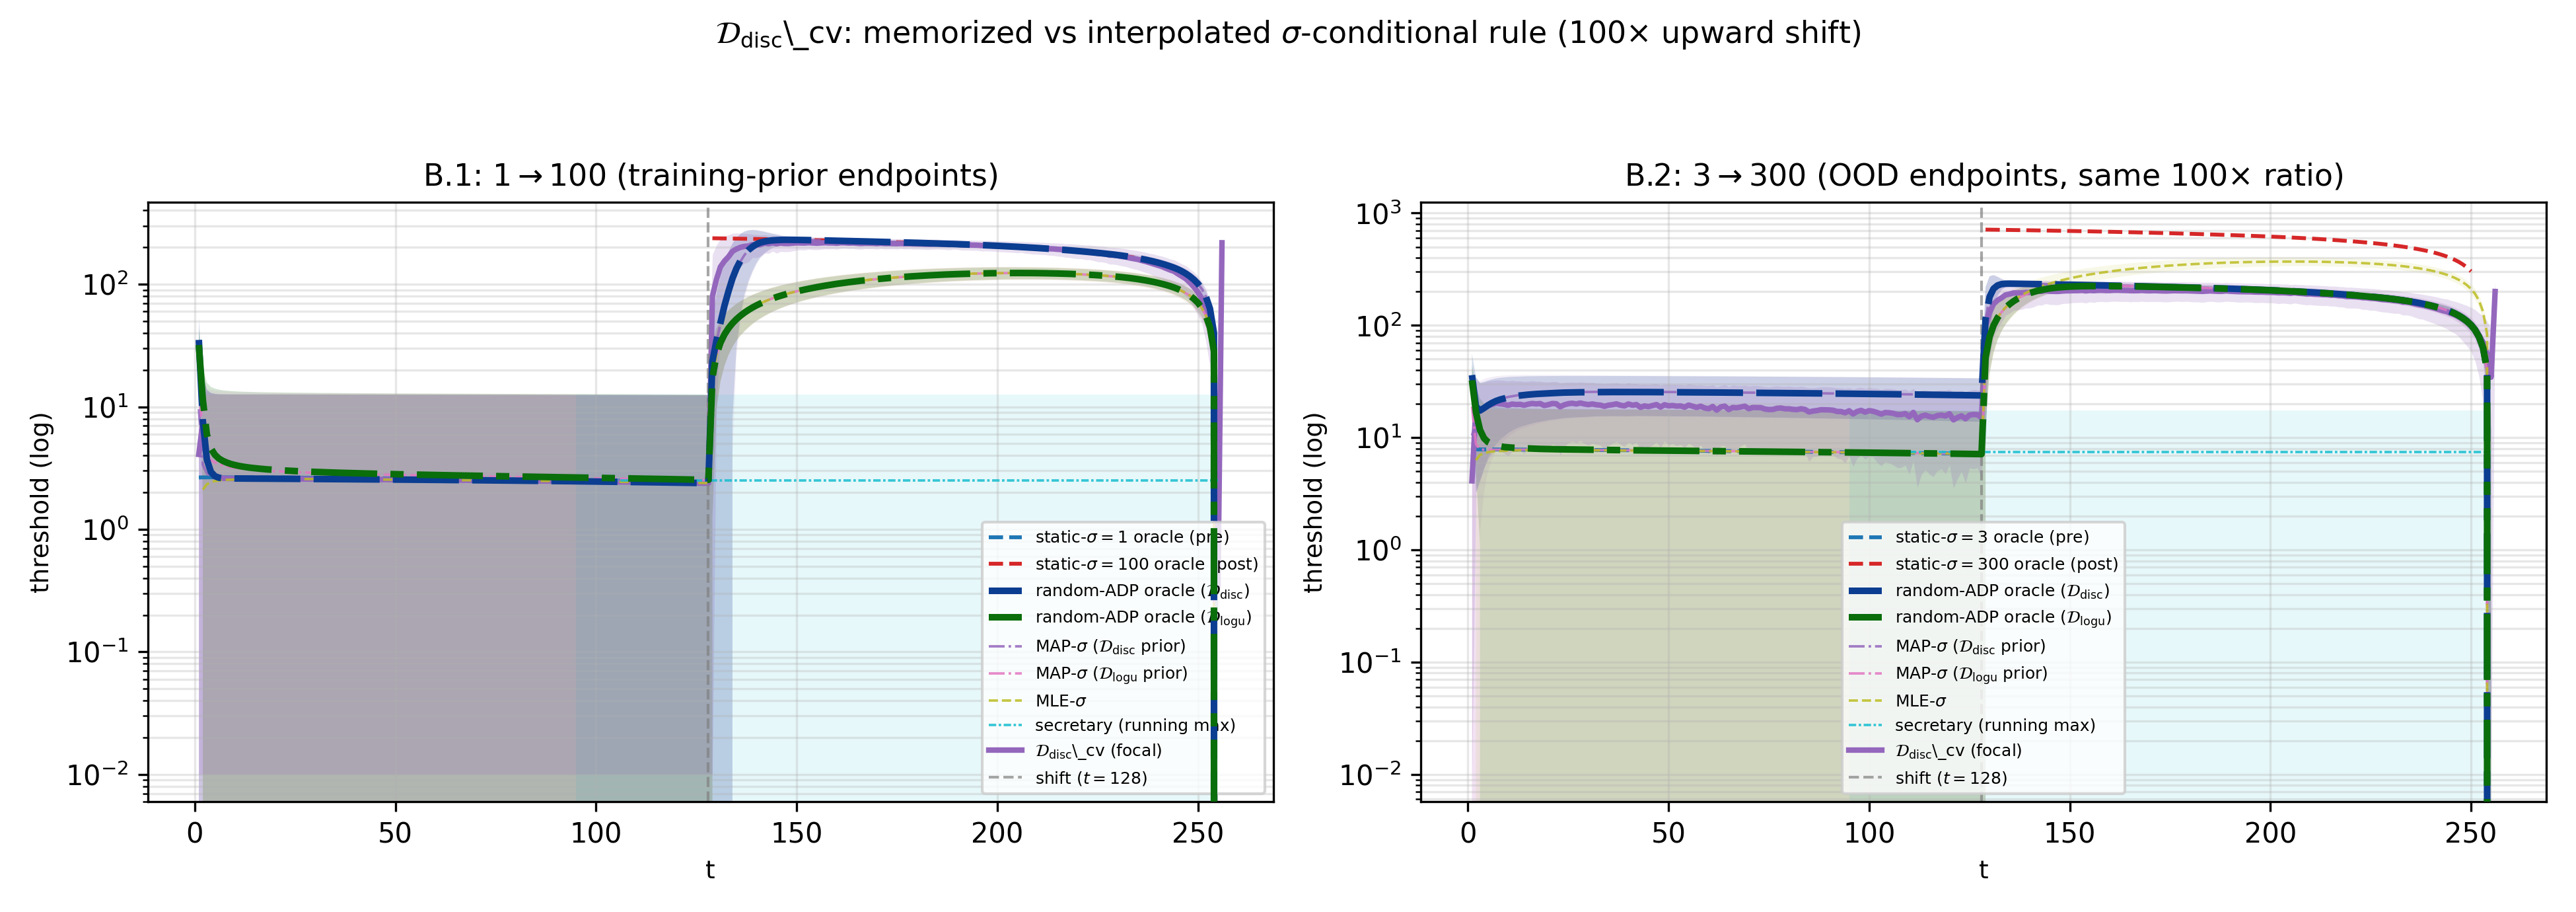
\includegraphics[width=\textwidth]{figures/sidebyside-1-100-vs-3-300-D_disc_cv.png}
\caption{Side-by-side trajectory comparison for $\mathcal{D}_{\mathrm{disc}}$\_cv on a $100\times$ upward shift: $1 \to 100$ (training-prior endpoints, B.1) vs.\ $3 \to 300$ (OOD endpoints, B.2). Same scale ratio, same direction; the OOD post-shift threshold saturates at the $\sigma = 100$ band rather than reaching the $\sigma = 300$ oracle.}
\label{fig:sidebyside-1-100-vs-3-300}
\end{figure}

\begin{figure}[H]
\centering
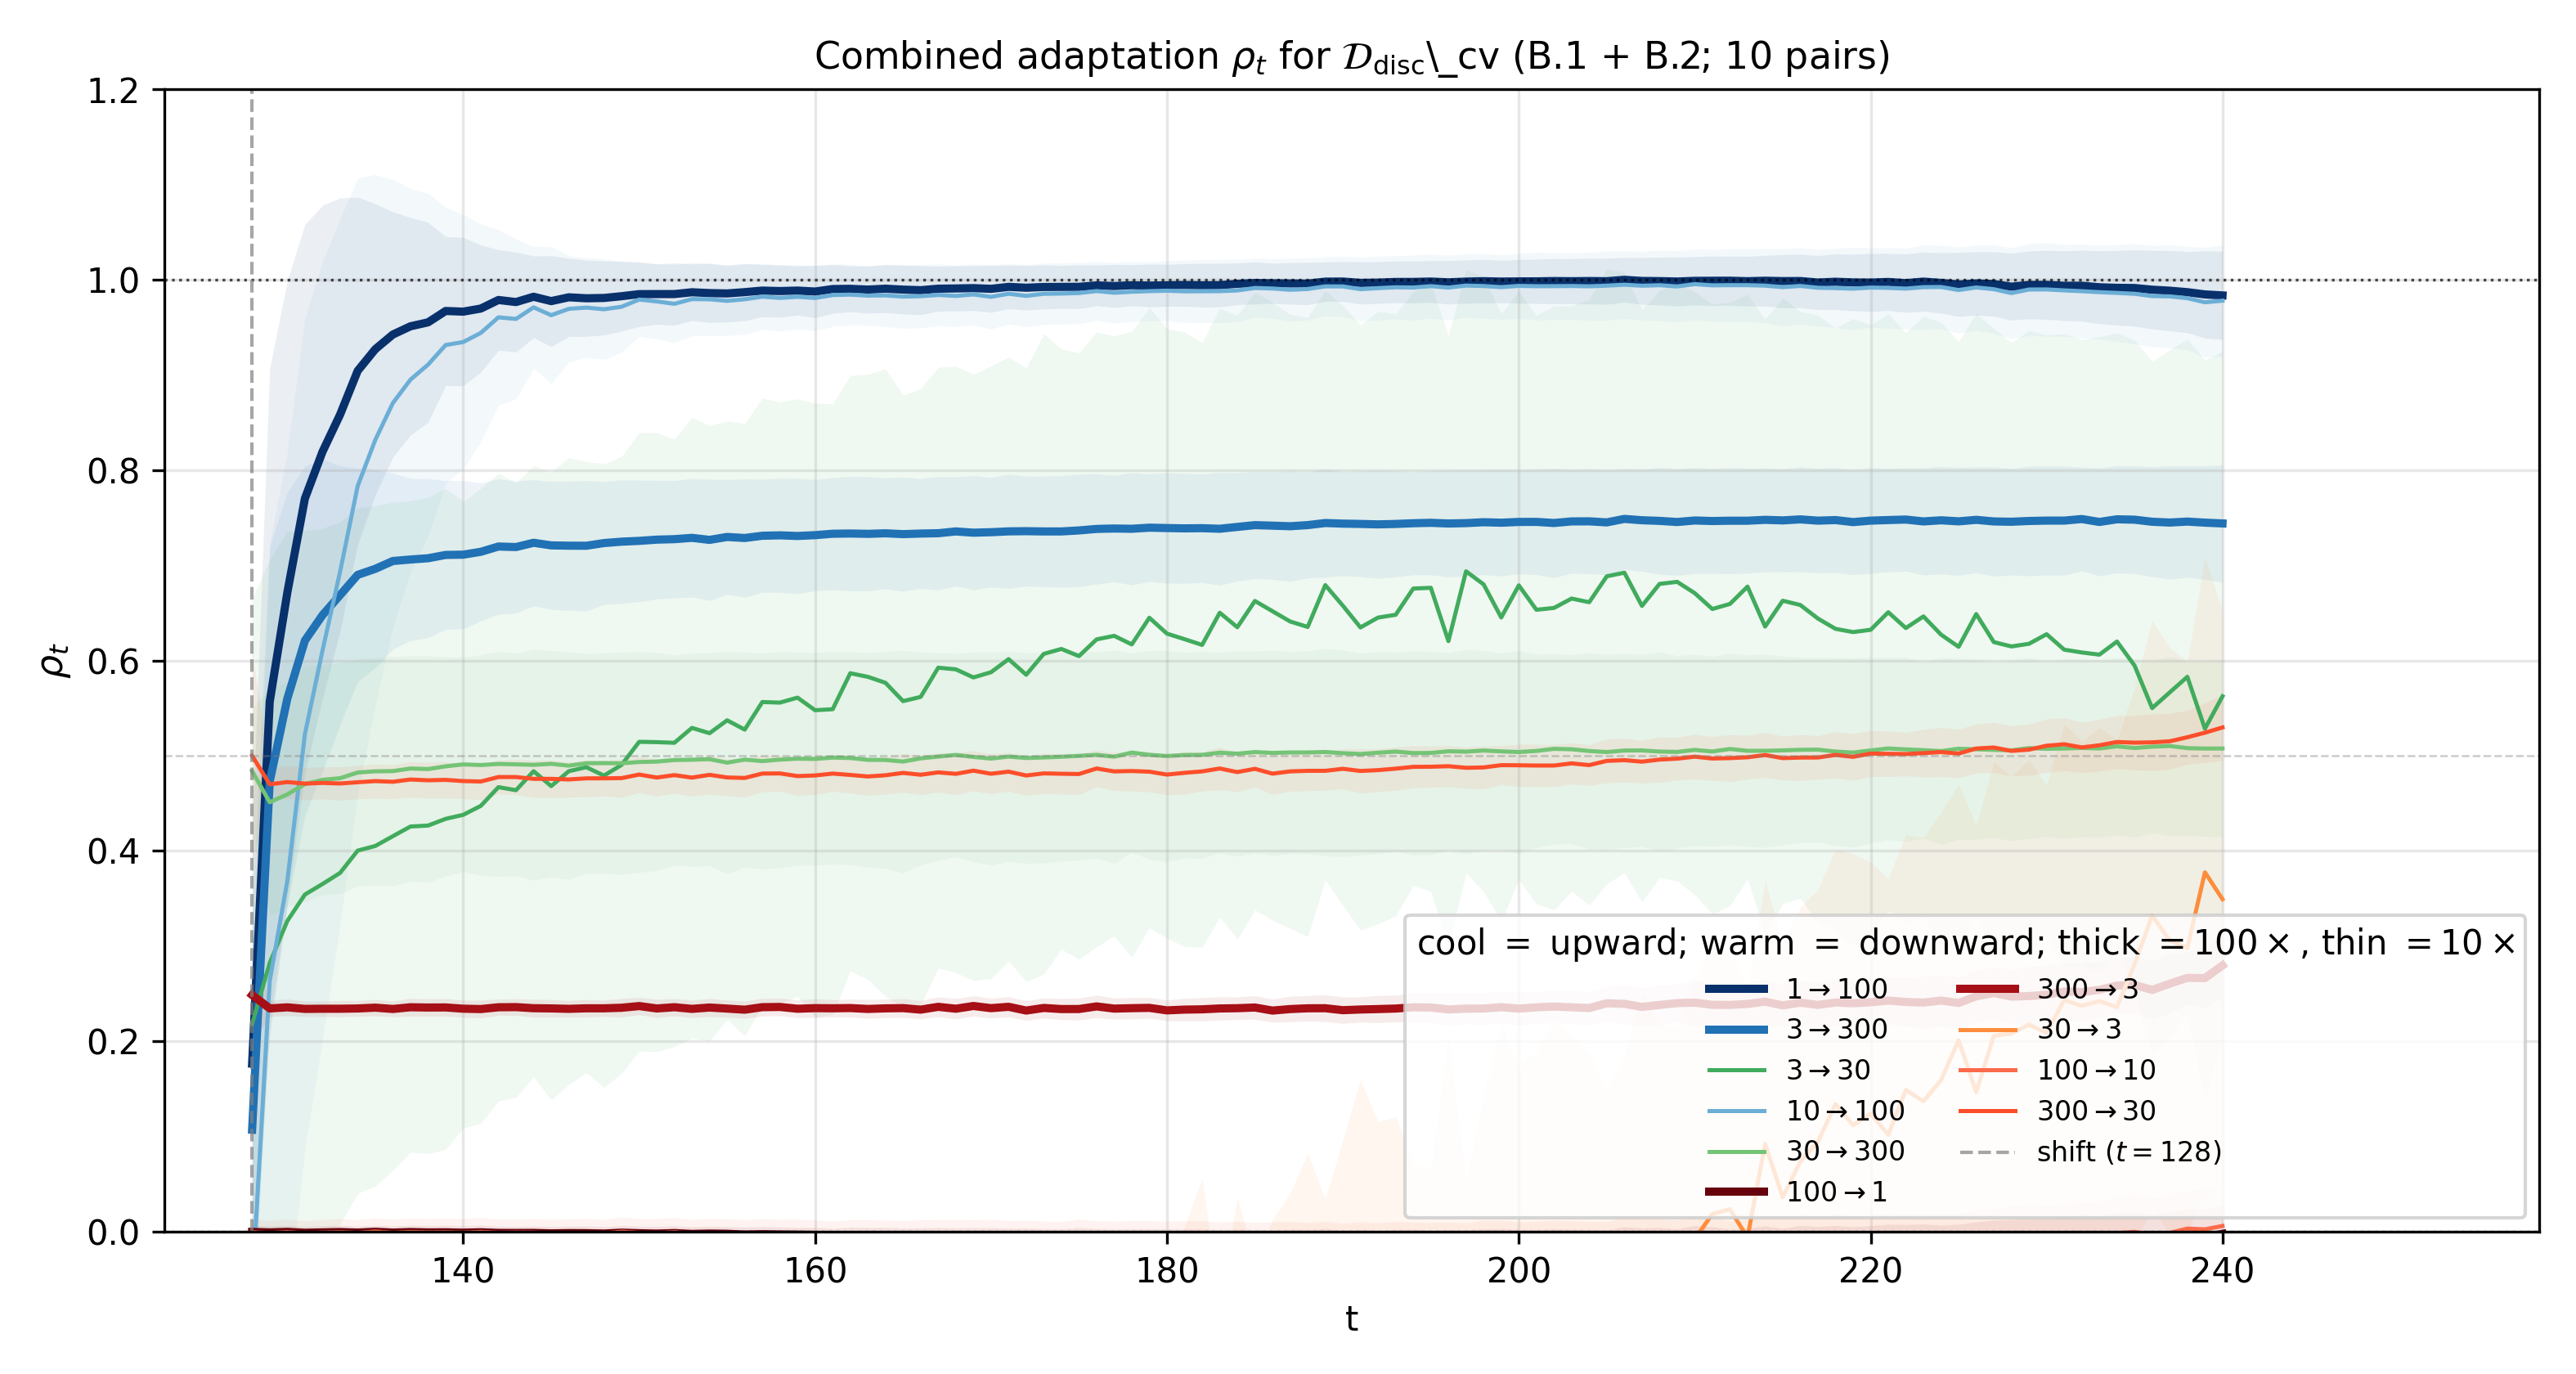
\includegraphics[width=0.49\textwidth]{figures/rho-shift-combined-D_disc_cv.png}\hfill
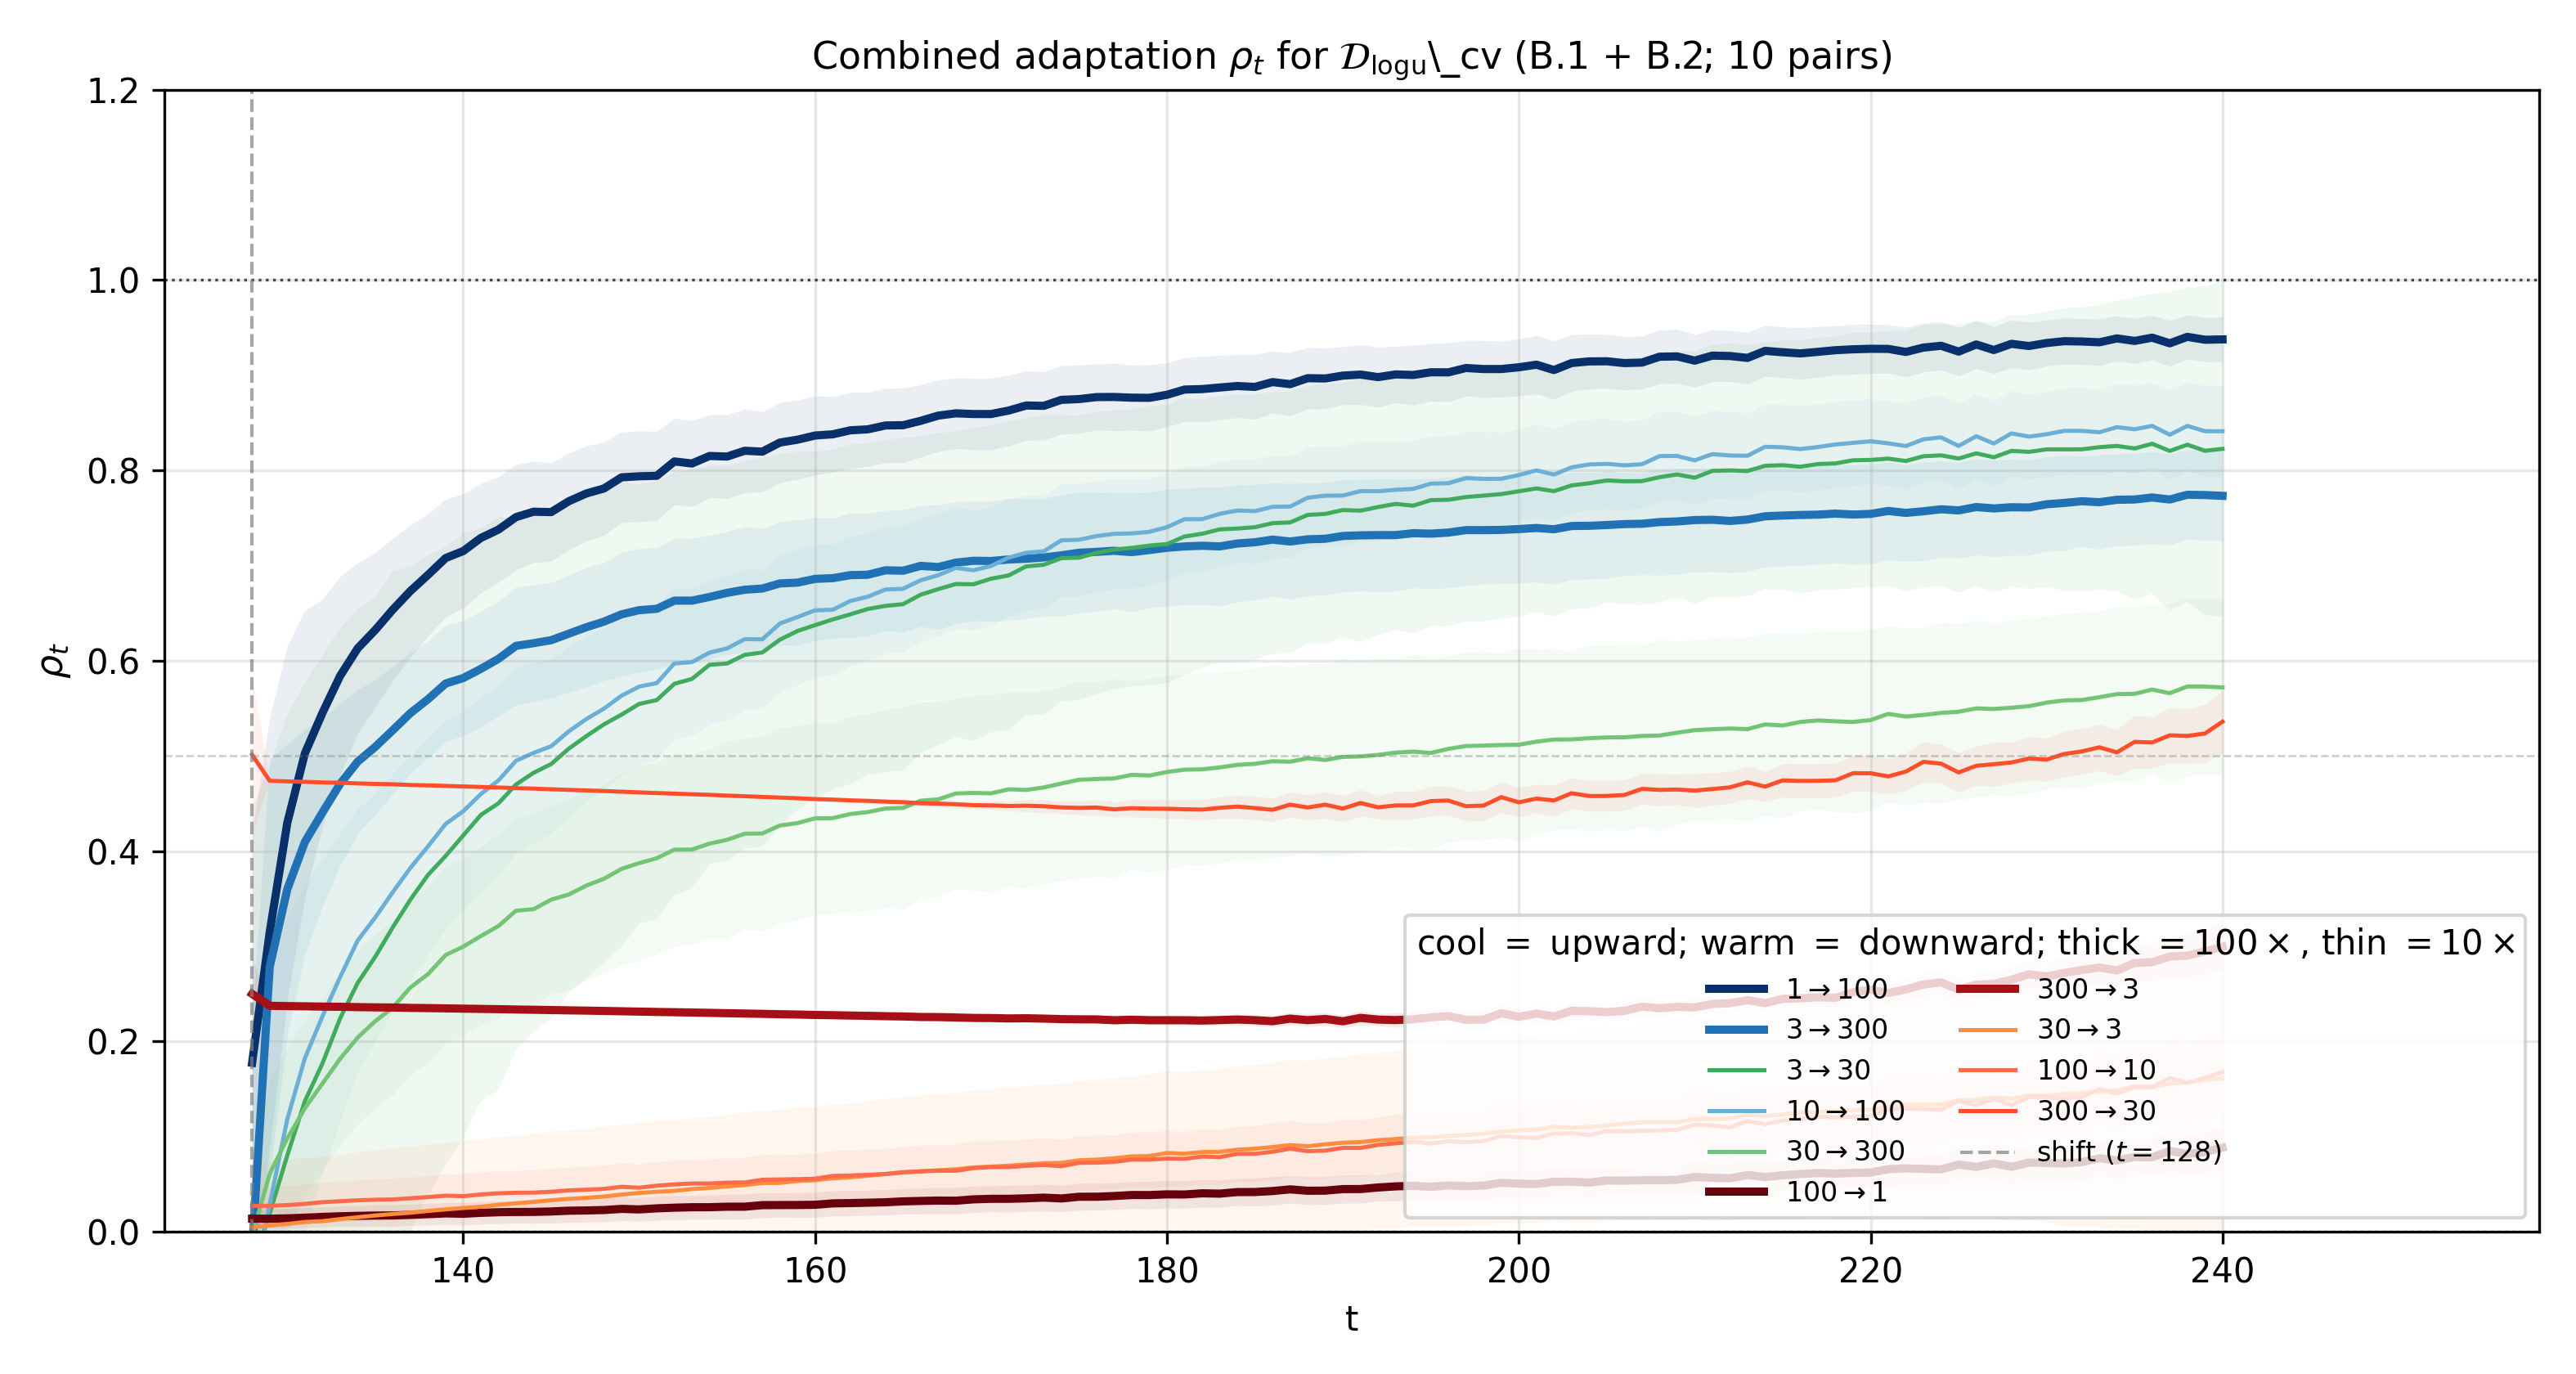
\includegraphics[width=0.49\textwidth]{figures/rho-shift-combined-D_logu_cv.png}
\caption{Combined adaptation $\rho_t$ across all ten pairs (B.1 $+$ B.2), $t \in [128, 240]$. Left: $\mathcal{D}_{\mathrm{disc}}$\_cv. Right: $\mathcal{D}_{\mathrm{logu}}$\_cv. Cool $=$ upward shifts; warm $=$ downward; thick $=$ $100\times$ ratio, thin $=$ $10\times$.}
\label{fig:rho-combined-disc-logu}
\end{figure}

These regime-shift results are the clearest evidence of in-context adaptation: the trained models reset their $\sigma$-belief mid-sequence in response to the post-shift data, while every i.i.d.\ baseline plots a flat post-shift threshold by construction. Adaptation is asymmetric --- upward shifts settle within a few observations, downward shifts often miss $\rho = 0.5$ within the 128-step window. Two effects compound here. First, the problem itself is asymmetric: stopping at a maximum makes the optimal policy attend to large values (which determine when to accept) and largely ignore small ones, so the model's behaviour is naturally more responsive to the high tail than the low one. Second, Bayesian updating reinforces the same asymmetry --- a single high-$\sigma$ outlier moves the posterior fast, while a sequence of typical-magnitude observations changes the posterior only logarithmically.

\paragraph{Equal weighting of past observations.} Every baseline in Section~\ref{sec:baselines} is derived under the i.i.d.\ assumption: $X_{1:t}$ is treated as evidence for a single fixed (or fixed-mixture) distribution, so post-shift observations are diluted into the running statistics rather than overwriting them, and the post-shift threshold stays flat. The trained models inherit a milder version of the same bias --- training data contained no temporal shifts, so the network appears to weight all observations roughly equally rather than down-weight pre-shift evidence, producing the asymmetric adaptation noted above. Within this picture the $\sigma{=}1 \to 100$ gap between $\mathcal{D}_{\mathrm{disc}}$\_cv ($t_{1/2} = 1.8$, post-shift error $17.9$) and $\mathcal{D}_{\mathrm{logu}}$\_cv ($t_{1/2} = 3.2$, post-shift error $45.1$; Table~\ref{tab:res-shift-summary}, Figures~\ref{fig:traj-shift-disc-cv}--\ref{fig:traj-shift-logu-cv}) is a prior-shape effect: the disc prior places an atom at $\sigma = 100$ that the implicit posterior locks onto after a single large-magnitude observation, while the logu prior is continuous on $[1, 100]$ and concentrates somewhere near $\sigma \approx 80$--$90$, leaving the visible saturation-level threshold gap. A baseline or trained model that explicitly down-weighted observations older than some window $T$ would not be subject to either limitation.

\section{Mechanistic analysis}
\label{sec:probe}

A mechanistic question raised by Section~\ref{sec:results} is whether the trained random-variance models actually represent the quantities the algorithmic hypothesis would predict --- the sufficient statistics, posterior probabilities, the continuation value --- inside their internal activations, or whether they implement an opaque shortcut that produces the right outputs without the corresponding intermediates. We test this directly by training auxiliary regressors (probes) on the frozen models' hidden states.

\subsection{Setup}
\label{sec:probe-setup}

We freeze a trained model and train auxiliary probe networks to recover target quantities from its hidden states at each layer $\ell \in \{0, 1, \ldots, L\}$. The hidden state at position $t$ after block $\ell$ is denoted $\mathbf{h}_t^{(\ell)} \in \mathbb{R}^{d_{\mathrm{emb}}}$; we stack these across positions into the matrix
\[
H^{(\ell)} \;:=\; \begin{pmatrix} \mathbf{h}_1^{(\ell)} & \mathbf{h}_2^{(\ell)} & \cdots & \mathbf{h}_n^{(\ell)} \end{pmatrix}^{\!\top} \;\in\; \mathbb{R}^{n \times d_{\mathrm{emb}}}.
\]
Each block contributes additively rather than replacing the previous state, with causally masked attention so position $t$ sees only positions $1, \ldots, t$:
\[
\mathbf{h}_t^{(\ell)} \;=\; \mathbf{h}_t^{(\ell-1)} \;+\; \mathrm{Attn}^{(\ell)}\!\bigl(H_{1:t}^{(\ell-1)}\bigr)_t \;+\; \mathrm{MLP}^{(\ell)}\!\bigl(\mathbf{h}_t^{(\ell-1)} + \mathrm{Attn}^{(\ell)}(H_{1:t}^{(\ell-1)})_t\bigr).
\]
Unrolling the recursion gives
\[
\mathbf{h}_t^{(L)} \;=\; \mathbf{h}_t^{(0)} \;+\; \sum_{\ell=1}^{L} \boldsymbol\delta_t^{(\ell)}, \qquad \boldsymbol\delta_t^{(\ell)} := \mathbf{h}_t^{(\ell)} - \mathbf{h}_t^{(\ell-1)}.
\]
$\mathbf{h}_t^{(0)}$ is the input embedding plus positional embedding; each $\boldsymbol\delta_t^{(\ell)}$ is the contribution of block $\ell$, which depends only on $\mathbf{h}_{1:t}^{(\ell-1)}$. Probing at depth $\ell$ reads from the partial sum $\mathbf{h}_t^{(\ell)} = \mathbf{h}_t^{(0)} + \sum_{\ell' \le \ell} \boldsymbol\delta_t^{(\ell')}$ --- everything the first $\ell$ blocks have written, based only on past and present observations.

\paragraph{Probe.} For target $v_t$ (a scalar that depends on $X_{1:t}$), the per-timestep probe is
\[
\hat v_t \;=\; \mathrm{FF}\bigl(\mathbf{h}_t^{(\ell)}\bigr),
\]
with the same $\mathrm{FF}$ applied at every $(\text{sequence}, t)$ pair --- a shared head reused across timesteps rather than one head per $t$. This is the standard linear-probing choice; it gives per-$t$ predictions for free, and assumes the target lives in a consistent direction of $\mathbf{h}_t^{(\ell)}$ across $t$ (which the algorithmic hypothesis predicts, since the model is supposed to be running the same computation at every step). We train two $\mathrm{FF}$ variants per layer:
\begin{enumerate}
    \item a linear map $\mathbb{R}^{d_{\mathrm{emb}}} \to \mathbb{R}$,
    \item a 2-layer MLP with hidden width $512$ and GeLU activation.
\end{enumerate}
As a strictly more expressive variant we also train an attention-pooled probe
\[
\boldsymbol\alpha_t \;=\; \mathrm{softmax}\bigl((\mathbf{s}_v)_{1:t}\bigr) \in \Delta^{t-1}, \qquad
\hat v_t \;=\; \mathrm{FF}\!\Bigl(\textstyle\sum_{i=1}^t (\boldsymbol\alpha_t)_i \,W_v\,\mathbf{h}_i^{(\ell)}\Bigr),
\]
where $\mathbf{s}_v \in \mathbb{R}^n$ is a learned attention-score vector (shared across $t$, restricted to the first $t$ entries and softmax-normalized) and $W_v \in \mathbb{R}^{d_{\mathrm{emb}} \times d_{\mathrm{emb}}}$ is a learned projection. The probe's attention is causally masked and position-indexed but data-independent --- it does not vary with $X_{1:t}$. The attention-pooled form reduces to the per-timestep form when $\boldsymbol\alpha_t$ concentrates on position $t$; the gap between the two is diagnostic of whether the target lives only at position $t$ or is spread across the prefix and must be gathered, and the trained $\boldsymbol\alpha_t$ further indicates \emph{where} in the prefix the target lives. We report results for both forms in the single-shot analysis (Appendix~\ref{sec:probe-results}); the planned permutation test of Section~\ref{sec:probe-ensemble} uses only the simpler per-timestep probe, both to keep the probe expressivity below the encoded-feature complexity (a probe-expressivity defense in its own right) and to keep the ensemble compute tractable.

All probes are trained with per-$(\text{sequence}, t)$ MSE loss masked to $t \in \{2, \ldots, n - 1\}$. Adam at learning rate $10^{-3}$, batch size $256$, $3$ epochs (linear) or $5$ epochs (MLP); best-validation-loss checkpoint selected per probe.

\paragraph{Targets.} We probe three tiers of quantities, each computable from $X_{1:t}$ and known oracle parameters (Table~\ref{tab:probe-targets}). Probing the raw cumulants alongside their derived statistics localizes where each derivation circuit lives in depth (e.g.\ a $Q_t \to \hat\sigma_t^2$ saturation gap measures the variance-computation step); probing MAP and MLE separately discriminates whether the model uses its training prior or a pure sample SD; probing the log-likelihood at the true latent $\sigma_i$ (never seen as input) tests whether the model carries a parametric likelihood representation rather than memorized point evaluations. Probing the act-supervised models on $\widehat C_t^\star$ is the cleanest mechanistic test in the suite, since $\widehat C_t^\star$ never appears in their training signal.

\begin{table}[H]
\centering
\small
\renewcommand{\arraystretch}{1.25}
\begin{tabular}{l l p{0.42\textwidth}}
\hline
notation & definition & what it represents \\
\hline
\multicolumn{3}{l}{\textit{Tier 1 --- Sufficient statistics}} \\
$S_t$ & $\sum_{s \le t} X_s$ & cumulative sum of observations through $t$ \\
$Q_t$ & $\sum_{s \le t} X_s^2$ & cumulative sum of squared observations \\
$\bar X_t$ & $S_t / t$ & running sample mean (estimator of $\mu_i$) \\
$\hat\sigma_t^2$ & $\dfrac{1}{t-1}\sum_{s\le t}\bigl(X_s - \bar X_t\bigr)^2 = \dfrac{Q_t - t\,\bar X_t^2}{t-1}$ & Bessel-corrected running sample variance of $X_{1:t}$ (unbiased estimator of $\sigma_i^2$ under fixed $\mu_i$); defined for $t \ge 2$ \\
\hline
\multicolumn{3}{l}{\textit{Tier 2 --- Posterior probabilities and point estimates}} \\
$\hat\sigma_t^{\mathrm{MAP}}$ & $\displaystyle\arg\max_{\sigma}\bigl[\log p(X_{1:t}\mid\sigma) + \log p(\sigma)\bigr]$ & MAP-$\sigma$ under the model's training prior $p(\sigma)$ (3-pt discrete on $\mathcal{D}_{\mathrm{disc}}$, log-uniform on $\mathcal{D}_{\mathrm{logu}}$); marginal likelihood given by Eq.~\eqref{eq:marginal-loglik} \\
$s_t$ & $\sqrt{\hat\sigma_t^2} = \sqrt{\dfrac{Q_t - t\,\bar X_t^2}{t - 1}}$ & running sample standard deviation: a data-only, prior-free point estimator of $\sigma_i$. Used as the $\sigma$-estimate by the MLE-$\sigma$ plug-in baseline of Section~\ref{sec:baselines}; the baseline's ``MLE'' name is conventional (no $\sigma$-prior, as opposed to MAP-$\sigma$) rather than literal --- the strict maximum-likelihood estimator under $\mathcal{N}(\mu_i, \sigma_i^2)$ with unknown $\mu_i$ uses divisor $t$ instead of $t-1$, differing from $s_t$ by a factor of $\sqrt{t/(t-1)} = 1 + O(1/t)$. \\
$\log p(X_{1:t} \mid \sigma)$ & Eq.~\eqref{eq:marginal-loglik} at $\sigma \in \{1, 10, 100\}$ & log marginal likelihood at three fixed $\sigma$ values (one target each) \\
$\log p(X_{1:t} \mid \sigma_i)$ & Eq.~\eqref{eq:marginal-loglik} at $\sigma = \sigma_i$ & log marginal likelihood at the \emph{true} per-sequence latent (model never sees $\sigma_i$) \\
\hline
\multicolumn{3}{l}{\textit{Tier 3 --- Continuation value}} \\
$\widehat C_t^\star$ & Section~\ref{sec:oracle} ADP table for $\mathcal{D}_\mathrm{train}$ & Bayes-optimal continuation value under the model's training prior \\
$\widehat C_t^{\mathrm{plug\text{-}in,\,MAP}}$ & $\bar X_t + \hat\sigma_t^{\mathrm{MAP}}\,\eta_t$ & data-only plug-in threshold using MAP-$\sigma$ \\
$\widehat C_t^{\mathrm{plug\text{-}in,\,MLE}}$ & $\bar X_t + s_t\,\eta_t$ & data-only plug-in threshold (no $\sigma$-prior); conventionally called the ``MLE-$\sigma$ plug-in'' \\
\hline
\end{tabular}
\caption{Probe targets. All thirteen quantities are computed analytically from $X_{1:t}$ and known oracle parameters; probes are trained to recover each from the model's hidden state at every layer.}
\label{tab:probe-targets}
\end{table}

\paragraph{Control baselines.} Probe success conflates probe capacity, architectural bias, and training-induced structure. We report two single-shot noise floors that hold the probe fixed and vary the model representation:
\begin{itemize}
\item \emph{Random-init}: the same architecture with default PyTorch initialization and no training (per-distribution seed disjoint from every training seed). Strictest floor; isolates what the probe can extract from architecture and probe capacity alone.
\item \emph{Constant-label control}: same architecture trained on the same generative distribution for the act run's full step count, but with $y_t^{\mathrm{act}} = 0$ at every $t$. BCE drives every logit to $-\infty$, so the labels carry no $\sigma$-information, yet the model has been through the full training procedure. Stricter test: beating it means the probed feature is task-specific, not just architecture-plus-training-dynamics.
\end{itemize}
Per (model, target, layer) we report linear- and MLP-probe MSE on a $10^4$-sequence held-out test split, normalized as $\mathrm{nMSE} := \mathrm{test\ MSE}/\mathrm{Var}(\mathrm{target})$ so that $\mathrm{nMSE} = 1$ corresponds to the constant-mean baseline. The trained-vs-floor ratio at the best layer per target is the headline diagnostic.

Single-shot probe curves for both distributions, both probe variants (per-timestep and attention-pooled), and the cross-distribution overlay are reported in Appendix~\ref{sec:probe-results}; the discussion below uses them as descriptive context for the planned statistical test.

\subsection{Statistical grounding: a planned paired-ensemble permutation test}
\label{sec:probe-ensemble}

The two noise floors of Section~\ref{sec:probe-setup} are single-shot comparisons: they hold the probe and target fixed and vary only the model representation. They give no $p$-value, no confidence interval, no sense of how variable the trained-vs-floor gap is across initializations and dataset draws. To address this we plan a paired-bootstrap design with $N$ independent training pairs.

\paragraph{Phase 1 --- $N$ paired base-model trainings.} For $i = 1, \ldots, N$, draw seed $s_i$ and train two models with the same architecture and the same generative distribution but different labels:
\begin{itemize}
\item \emph{True}: trained with seed $s_i$ on the oracle act labels of Section~\ref{sec:labeling}.
\item \emph{Control}: trained with the same seed $s_i$ on a per-sequence permutation of the oracle's action labels. Identical input distribution and label marginal; only the input--label alignment is destroyed.
\end{itemize}
The shared seed within a pair controls initialization luck; variation across pairs reflects training stochasticity.

\paragraph{Phase 2 --- probing.} Freeze all $2N$ models. For each pair $i$, sample $50{,}000 + 5{,}000 + 10{,}000$ disjoint probe train/val/test sequences from the same distribution (seed disjoint from $s_i$), cache the layer-$\ell$ hidden states $\mathbf{h}_t^{(\ell)}$ for both models, and train the simpler per-timestep probe of Section~\ref{sec:probe-setup} (both linear and MLP $\mathrm{FF}$ variants) on each. The per-$(\text{sequence}, t)$ MSE is recorded for both true and control probes at each (target, layer):
\[
\mathrm{MSE}^{\mathrm{true}}_{i,\,v,\,\ell,\,t}, \qquad \mathrm{MSE}^{\mathrm{ctrl}}_{i,\,v,\,\ell,\,t}.
\]
The shared-across-$t$ probe form already produces a per-$t$ prediction $\hat v_t$, so per-timestep resolution comes from breaking out this MSE rather than training a separate probe per $t$. For display we summarise at a representative grid $t \in \{8, 32, 64, 128, 192, 240\}$.

\paragraph{Phase 2b --- per-prefix-length probes (supplementary).} The shared-across-$t$ probe assumes a $t$-invariant encoding direction; if the model rotates its encoding with $t$, it will under-report nMSE. As a cross-check we train fixed-$t^\star$ probes at $t^\star \in \{25, 125, 250\}$ (short, medium, long horizon): one $\mathrm{FF}_{t^\star}$ per $(\ell, t^\star)$, fit on $\{(\mathbf{h}_{t^\star}^{(\ell)}, v_{t^\star})\}$ from the probe split. Concordance with the shared probe at the same $t^\star$ supports $t$-invariance; a large per-$t^\star$ advantage flags a rotating direction. Compute precludes running the full $N = 100$ ensemble at every $t^\star$, so these are reported as descriptive curves only.

\paragraph{Phase 3 --- statistical inference per cell.} For each (target, layer, $t$) cell we have $N$ paired observations and report two complementary statistics.

\textit{Binomial sign test.} Let $W := \sum_{i=1}^N \mathbb{I}[\mathrm{MSE}^{\mathrm{ctrl}}_i < \mathrm{MSE}^{\mathrm{true}}_i]$ count how often the control beats the true model. Under the null of exchangeability $W \sim \mathrm{Binomial}(N, 1/2)$, and the empirical $p$-value is $\Pr[W \le w_{\mathrm{obs}}]$. Rendered as a per-cell heatmap of $\log p$.

\textit{Paired confidence interval.} Define the per-pair improvement $\Delta_i := \mathrm{MSE}^{\mathrm{ctrl}}_i - \mathrm{MSE}^{\mathrm{true}}_i$; report the 95\% interval $\bar\Delta \pm 1.96\,\mathrm{SE}(\bar\Delta)$ with $\mathrm{SE} = N^{-1/2}\,\mathrm{sd}(\Delta)$. A CI comfortably above zero is direct evidence that the act training objective \emph{causally} forced the network to encode the target. The sign test answers ``how often is true better''; the CI answers ``by how much.''

\textit{Significance threshold under multiple comparisons.} The dense grid contains roughly $13~\text{targets} \times (L+1) = 9~\text{layers} \times 6~\text{time-bins} \approx 700$ cells per (distribution, $\mathrm{FF}$ variant). Uncorrected $\alpha = 0.05$ would expect $\sim 35$ false positives by chance and is not informative for individual cells. We adopt the family-wise Bonferroni-corrected threshold $\alpha_{\mathrm{cell}} = 0.05/k$ as the headline criterion. The tail probabilities of $\mathrm{Binomial}(N = 100,\, 1/2)$ are
\[
\Pr[W \ge 67] \approx 4.4\!\times\!10^{-4}, \quad
\Pr[W \ge 68] \approx 2.3\!\times\!10^{-4}, \quad
\Pr[W \ge 69] \approx 1.1\!\times\!10^{-4}, \quad
\Pr[W \ge 70] \approx 4.8\!\times\!10^{-5},
\]
so the Bonferroni-corrected significance thresholds are $W \ge 67$ for the headline target $\times$ layer grid ($k = 117$, $\alpha_{\mathrm{cell}} = 4.3\!\times\!10^{-4}$), $W \ge 69$ for the time-resolved grid ($k \approx 300$, $\alpha_{\mathrm{cell}} = 1.7\!\times\!10^{-4}$), and $W \ge 70$ for the full grid including both probe variants ($k \approx 700$, $\alpha_{\mathrm{cell}} = 7\!\times\!10^{-5}$). Cells in the uncorrected $p < 0.001$ band ($66 \le W \le 67$) are not reported as significant in isolation; we treat coherent clusters across adjacent layers or related targets as stronger evidence than isolated peaks even at $W = 70$, since neighbouring cells share representational support and cannot be produced independently by chance. Exact per-cell $p$-values are reported in full so that readers can apply Benjamini--Hochberg false-discovery control or any preferred alternative correction.

\paragraph{Design choices and compute estimate.} We plan $N = 100$ on $\mathcal{D}_{\mathrm{logu}}$ first; if decisive on the headline targets, the result is reported and $\mathcal{D}_{\mathrm{disc}}$ is treated as a planned replication. To keep the budget manageable, ensemble members are trained for $5 \times 10^4$ steps rather than the full $1.5 \times 10^5$ of the headline runs --- the relevant $\sigma$-aware features emerge by step $\sim 3 \times 10^4$ in the existing training curves, and we will sanity-check on a single pair before launching the full sweep. At $\sim$50 minutes per model, $N = 100$ is $\sim 170$ GPU-hours, roughly two days wall on four GPUs in the best case.

\bibliographystyle{plainnat}
\bibliography{references}

\appendix

\section{Approximate dynamic programming for the oracle}
\label{app:adp}

This appendix details the discretized backward-induction procedure used to label training data and to build the per-regime optimal threshold $R^\star$. We treat the static-variance and random-variance cases separately, then describe the convergence diagnostic.

\subsection{Static-variance ADP}
\label{app:adp-static}

\paragraph{Sufficient statistic and posterior.} The sufficient statistic for $\mu$ given $X_{1:t}$ is the running sum $S_t := \sum_{s=1}^t X_s$, equivalently the sample mean $\bar X_t = S_t/t$. The conjugate Normal--Normal posterior depends on $X_{1:t}$ only through $S_t$:
\begin{equation}
\label{eq:mu-static}
\mu \mid X_{1:t} \;\sim\; \mathcal{N}(\mu_t, \tau_t^2),
\qquad
\tau_t^2 = \!\left(\frac{1}{\tau_0^2} + \frac{t}{\sigma^2}\right)^{\!-1},
\qquad
\mu_t = \tau_t^2\!\left(\frac{\mu_0}{\tau_0^2} + \frac{S_t}{\sigma^2}\right).
\end{equation}
$\tau_t^2$ is deterministic in $t$; $\mu_t$ is a deterministic function of $(t, S_t)$. The belief state is $b_t = \mu_t$, one-dimensional.

\begin{proof}[Derivation of \eqref{eq:mu-static}]
By Bayes' rule, $$p(\mu \mid X_{1:t}) \propto p(\mu)\, \prod_{s \le t} p(X_s \mid \mu, \sigma) \propto \exp\!\big[-\tfrac{(\mu-\mu_0)^2}{2\tau_0^2} - \tfrac{1}{2\sigma^2}\sum_s (X_s - \mu)^2\big].$$ The exponent is quadratic in $\mu$ with $\mu^2$ coefficient $-\tfrac{1}{2}(\tau_0^{-2} + t\sigma^{-2})$ and $\mu^1$ coefficient $\mu_0/\tau_0^2 + S_t/\sigma^2$. Completing the square in $\mu$ gives a Gaussian density with variance $\tau_t^2 = (\tau_0^{-2} + t\sigma^{-2})^{-1}$ and mean $\mu_t = \tau_t^2(\mu_0/\tau_0^2 + S_t/\sigma^2)$.
\end{proof}

\paragraph{DP recursion.} The continuation value satisfies $V_t(b_t, X_t) = \max\{X_t, C_t(\mu_t)\}$ for $t < n$ and $V_n = X_n$, with
\begin{equation}
\label{eq:Crec-static}
C_t(\mu_t) \;=\; \mathbb{E}_{X \sim \mathcal{N}(\mu_t,\, \tau_t^2 + \sigma^2)}\!\Big[\max\!\big\{X,\, C_{t+1}(\mathrm{update}(\mu_t, X))\big\}\Big],
\end{equation}
where $\mathrm{update}(\mu, X) = \alpha_t \mu + (1 - \alpha_t) X$ with $\alpha_t := \sigma^2/(\tau_t^2 + \sigma^2)$, and $C_{n-1}(\mu) = \mu$. The Bayes-optimal policy is $\pi^\star_{\mathcal{D}_i, t}(b_t, X_t) = \mathbf{1}[X_t \ge C_t(\mu_t)]$.

\begin{proof}[Derivation of the Bellman recursion]
At each $t < n$ the agent chooses between stopping (collect $X_t$, value $X_t$) and continuing (advance to $t+1$, where the same optimization repeats); at $t = n$ the agent must stop and collects $X_n$. Optimality gives $V_t(b_t, X_t) = \max\{X_t,\, \mathbb{E}[V_{t+1}(b_{t+1}, X_{t+1}) \mid b_t]\}$, and defining $C_t(b_t) := \mathbb{E}[V_{t+1} \mid b_t]$ as the continuation value yields the stated form. The expectation in~\eqref{eq:Crec-static} is over the one-step predictive $X_{t+1} \mid X_{1:t} \sim \mathcal{N}(\mu_t, \tau_t^2 + \sigma^2)$ --- a Gaussian with the posterior mean $\mu_t$ and marginal variance equal to the posterior variance $\tau_t^2$ (uncertainty in $\mu$) plus the observation noise $\sigma^2$. The terminal condition $C_{n-1}(\mu) = \mathbb{E}[V_n \mid X_{1:n-1}] = \mathbb{E}[X_n \mid X_{1:n-1}] = \mu_{n-1}$ is just the one-step predictive mean.
\end{proof}

\begin{proof}[Derivation of $\mathrm{update}(\mu, X)$]
With the time-$t$ posterior $\mu \mid X_{1:t} \sim \mathcal{N}(\mu_t, \tau_t^2)$ acting as a prior and a fresh observation $X_{t+1} \mid \mu \sim \mathcal{N}(\mu, \sigma^2)$, Bayes' rule gives
\[
p(\mu \mid X_{1:t+1}) \;\propto\; p(\mu \mid X_{1:t})\, p(X_{t+1} \mid \mu)
\;\propto\; \exp\!\left[-\frac{(\mu - \mu_t)^2}{2\tau_t^2} - \frac{(X_{t+1} - \mu)^2}{2\sigma^2}\right].
\]
Completing the square in $\mu$ collects the quadratic coefficient $\tau_{t+1}^{-2} = \tau_t^{-2} + \sigma^{-2}$ and the linear coefficient $\mu_t/\tau_t^2 + X_{t+1}/\sigma^2$, so
\[
\mu_{t+1} \;=\; \tau_{t+1}^2\!\left(\frac{\mu_t}{\tau_t^2} + \frac{X_{t+1}}{\sigma^2}\right)
\;=\; \frac{\sigma^2 \mu_t + \tau_t^2 X_{t+1}}{\tau_t^2 + \sigma^2}
\;=\; \alpha_t \mu_t + (1 - \alpha_t)\, X_{t+1},
\]
using $\tau_{t+1}^2 = \tau_t^2 \sigma^2/(\tau_t^2 + \sigma^2)$ and the stated definition of $\alpha_t$. The posterior mean at $t{+}1$ is therefore a convex combination of the previous posterior mean and the new observation, with weights set by the relative precisions of the two: $\alpha_t \to 1$ when the prior is much sharper than the likelihood ($\tau_t^2 \ll \sigma^2$) and $\alpha_t \to 0$ in the opposite limit.
\end{proof}

\paragraph{Discretization and quadrature.} Equation~\eqref{eq:Crec-static} has no elementary closed form. We discretize $\mu_t$ on a uniform grid of $K$ points covering $[\mu_0 - 5 s_t,\, \mu_0 + 5 s_t]$ at each stage, where $s_t = \sqrt{\tau_0^2 - \tau_t^2}$ is the marginal standard deviation of $\mu_t$ across sequences. The Gaussian expectation in~\eqref{eq:Crec-static} is approximated by $J$-point Gauss--Hermite quadrature, the standard rule for integrals against $e^{-z^2}$. The nodes $\{z_j\}_{j=1}^J \subset \mathbb{R}$ are the roots of the $J$-th physicists' Hermite polynomial $H_J$, and the weights $\{w_j\}_{j=1}^J > 0$ are uniquely determined by requiring that
\[
\int_{-\infty}^\infty f(z)\, e^{-z^2}\, dz \;\approx\; \sum_{j=1}^J w_j\, f(z_j)
\]
hold with equality whenever $f$ is a polynomial of degree at most $2J - 1$. Both nodes and weights depend only on $J$ and are precomputed (e.g., via \texttt{numpy.polynomial.hermite.hermgauss}). Substituting $X = \mu + \sqrt{2 v_t}\,z$ for $X \sim \mathcal{N}(\mu, v_t)$ with $v_t := \tau_t^2 + \sigma^2$ gives
\begin{equation}
\label{eq:gh}
\mathbb{E}_{X \sim \mathcal{N}(\mu, v_t)}[f(X)] \;\approx\; \frac{1}{\sqrt\pi}\sum_{j=1}^J w_j\, f\!\left(\mu + \sqrt{2 v_t}\, z_j\right).
\end{equation}
The factor $1/\sqrt\pi$ comes from the change of variables: with $z = (X - \mu)/\sqrt{2 v_t}$, the Gaussian density $(2\pi v_t)^{-1/2} e^{-(X-\mu)^2/(2 v_t)}\, dX$ becomes $\pi^{-1/2} e^{-z^2}\, dz$, so $\mathbb{E}[f(X)] = \pi^{-1/2}\!\int f(\mu + \sqrt{2 v_t}\,z)\, e^{-z^2}\, dz$, and Gauss--Hermite approximates the inner integral.
Off-grid values of $\widehat C_{t+1}$ are looked up by linear interpolation with clipping at the grid boundary. Algorithm~\ref{alg:adp-static} runs the backward induction at $K = 2048$, $J = 128$.

\begin{algorithm}[H]
\caption{Approximate DP for the static-variance Bayes-optimal threshold (per regime).}
\label{alg:adp-static}
\begin{algorithmic}[1]
\State Precompute $\tau_t^2, v_t := \tau_t^2 + \sigma^2, \alpha_t$ for each $t$; grid $\{m_t^{(k)}\}_{k=1}^K$ at each $t$; Gauss--Hermite nodes $\{(z_j, w_j)\}_{j=1}^J$
\State $\widehat C_{n-1}(m_{n-1}^{(k)}) \gets m_{n-1}^{(k)}$ for $k = 1, \ldots, K$
\For{$t = n-2, n-3, \ldots, 1$}
  \For{$k = 1, \ldots, K$}
    \State $S \gets 0$
    \For{$j = 1, \ldots, J$}
      \State $x_j \gets m_t^{(k)} + \sqrt{2 v_t}\, z_j$
      \State $\mu_j' \gets \alpha_t\, m_t^{(k)} + (1-\alpha_t)\, x_j$
      \State $S \gets S + w_j\, \max\!\big\{x_j,\, \widehat C_{t+1}^{\mathrm{lin}}(\mu_j')\big\}$
    \EndFor
    \State $\widehat C_t(m_t^{(k)}) \gets S/\sqrt\pi$
  \EndFor
\EndFor
\State \Return $\{\widehat C_t\}$
\end{algorithmic}
\end{algorithm}

\subsection{Random-variance ADP}
\label{app:adp-random}

\paragraph{Sufficient statistics.} The sufficient statistics for the joint posterior on $(\mu, \sigma)$ are
\begin{equation}
\label{eq:S-Q-defs}
S_t \;:=\; \sum_{s=1}^t X_s,
\qquad
Q_t \;:=\; \sum_{s=1}^t X_s^2.
\end{equation}
Both update online: $S_t = S_{t-1} + X_t$, $Q_t = Q_{t-1} + X_t^2$. Together with $t$, the pair $(S_t, Q_t)$ determines the joint posterior $p(\mu, \sigma \mid X_{1:t})$. $S_t$ alone determines the sample mean $\bar X_t = S_t/t$; jointly $(S_t, Q_t)$ determine the within-sequence sample variance
\[
\hat\sigma_t^2 \;:=\; \frac{1}{t-1}(Q_t - t\bar X_t^2).
\]

\begin{proof}[Why $(S_t, Q_t)$ are jointly sufficient, and the sample-variance identity]
The Gaussian log-likelihood expands as
\[
\log p(X_{1:t} \mid \mu, \sigma) = -\tfrac{t}{2}\log(2\pi\sigma^2) - \tfrac{1}{2\sigma^2}\!\sum_s (X_s - \mu)^2
= -\tfrac{t}{2}\log(2\pi\sigma^2) - \tfrac{1}{2\sigma^2}\big(Q_t - 2\mu S_t + t\mu^2\big),
\]
which depends on $X_{1:t}$ only through $(S_t, Q_t)$; by the Fisher--Neyman factorization, $(S_t, Q_t)$ are jointly sufficient for $(\mu, \sigma)$. The same expansion at $\mu = \bar X_t$ gives the sample-variance identity: $\sum_s (X_s - \bar X_t)^2 = Q_t - 2\bar X_t \cdot t \bar X_t + t \bar X_t^2 = Q_t - t \bar X_t^2$, and dividing by $t-1$ yields $\hat\sigma_t^2$.
\end{proof}

\paragraph{Joint posterior.} By Bayes' rule,
\[
p(\mu, \sigma \mid X_{1:t}) \;\propto\; p(\sigma)\, p(\mu)\, p(X_{1:t} \mid \mu, \sigma),
\]
which factors as $p(\sigma \mid X_{1:t}) \cdot p(\mu \mid X_{1:t}, \sigma)$. For any fixed $\sigma$, the conditional posterior $p(\mu \mid X_{1:t}, \sigma)$ is the standard Normal--Normal posterior~\eqref{eq:mu-static}: depends on $X_{1:t}$ only through $S_t$, with different $\sigma$ giving different conditional means and variances. The marginal posterior $p(\sigma \mid X_{1:t}) \propto p(\sigma)\, p(X_{1:t} \mid \sigma)$ uses the closed-form marginal log-likelihood~\eqref{eq:marginal-loglik}, derived as follows. For $\mathcal{D}_{\mathrm{disc}}$ the resulting posterior over $\sigma$ is a categorical on three points; for $\mathcal{D}_{\mathrm{logu}}$ a continuous density on $[1, 100]$.

\begin{proof}[Derivation of equation~\eqref{eq:marginal-loglik}]\label{app:marginal-derivation}
\textit{Step 1: marginal law.} Given $\sigma$, the joint $(\mu, X_{1:t})$ is Gaussian with $\mu \sim \mathcal{N}(\mu_0, \tau_0^2)$ and $X_s \mid \mu \sim \mathcal{N}(\mu, \sigma^2)$ independent across $s$. Marginalizing out $\mu$ keeps $X_{1:t}$ Gaussian. Its mean is $\mathbb{E}[X_s] = \mu_0 = 0$, and by the law of total covariance
\[
\mathrm{Cov}(X_r, X_s) \;=\; \mathbb{E}[\mathrm{Cov}(X_r, X_s \mid \mu)] + \mathrm{Cov}(\mathbb{E}[X_r \mid \mu], \mathbb{E}[X_s \mid \mu]) \;=\; \sigma^2\,\delta_{rs} + \tau_0^2,
\]
so $X_{1:t} \mid \sigma \sim \mathcal{N}(\mathbf{0}, \Sigma_t^{(\sigma)})$ with $\Sigma_t^{(\sigma)} = \sigma^2 I_t + \tau_0^2 \mathbf{1}\mathbf{1}^\top$.

\textit{Step 2: log-density via Sherman--Morrison.} Substituting into the Gaussian log-density gives
\[
\log p(X_{1:t} \mid \sigma) \;=\; -\tfrac{t}{2}\log(2\pi) - \tfrac{1}{2}\log\det\Sigma_t^{(\sigma)} - \tfrac{1}{2}\, X_{1:t}^\top \big(\Sigma_t^{(\sigma)}\big)^{\!-1} X_{1:t}.
\]
The matrix $\Sigma_t^{(\sigma)} = \sigma^2 I_t + \tau_0^2 \mathbf{1}\mathbf{1}^\top$ is a rank-one update of $\sigma^2 I_t$, so the matrix determinant lemma and the Sherman--Morrison formula give
\[
\log\det\Sigma_t^{(\sigma)} \;=\; t\log\sigma^2 + \log\!\left(1 + \tfrac{t\tau_0^2}{\sigma^2}\right),
\qquad
\big(\Sigma_t^{(\sigma)}\big)^{\!-1} \;=\; \frac{1}{\sigma^2}\, I_t - \frac{\tau_0^2/\sigma^4}{1 + t\tau_0^2/\sigma^2}\,\mathbf{1}\mathbf{1}^\top.
\]
Using $X_{1:t}^\top I_t X_{1:t} = Q_t$ and $X_{1:t}^\top \mathbf{1}\mathbf{1}^\top X_{1:t} = S_t^2$, the quadratic form becomes
\[
X_{1:t}^\top \big(\Sigma_t^{(\sigma)}\big)^{\!-1} X_{1:t} \;=\; \frac{Q_t}{\sigma^2} - \frac{\tau_0^2\, S_t^2/\sigma^4}{1 + t\tau_0^2/\sigma^2}.
\]
Assembling the three terms yields~\eqref{eq:marginal-loglik}, with the additive $-\tfrac{t}{2}\log(2\pi)$ absorbed into $\mathrm{const}(t)$. The $X$-dependence enters only through $(S_t, Q_t)$.
\end{proof}

\paragraph{Predictive distribution and DP recursion.} The predictive $p(X_{t+1} \mid X_{1:t})$ is a mixture of Gaussians with weights from $p(\sigma \mid X_{1:t})$:
\begin{equation}
\label{eq:predictive}
p(X_{t+1} \mid X_{1:t}) \;=\; \int p(\sigma \mid X_{1:t}) \cdot \mathcal{N}\!\left(X_{t+1};\, \mu_t^{(\sigma)},\, v_t^{(\sigma)}\right)\, d\sigma,
\qquad v_t^{(\sigma)} := \tau_t^{2,(\sigma)} + \sigma^2,
\end{equation}
with the integral replaced by a sum over $\{1, 10, 100\}$ for $\mathcal{D}_{\mathrm{disc}}$. The belief state is $b_t = (S_t, Q_t)$. Backward induction gives $V_t(b_t, X_t) = \max\{X_t, C_t(b_t)\}$ for $t < n$ with $V_n = X_n$, and
\begin{equation}
\label{eq:Crec-random}
C_t(b_t) \;=\; \mathbb{E}_{X_{t+1} \sim p(\cdot \mid b_t)}\!\big[\max\{X_{t+1}, C_{t+1}(b_{t+1})\}\big],
\end{equation}
expectation over the mixture predictive~\eqref{eq:predictive}, $b_{t+1} = (S_t + X_{t+1}, Q_t + X_{t+1}^2)$, terminal $C_{n-1}(b_{n-1}) = \int p(\sigma \mid X_{1:n-1}) \mu_{n-1}^{(\sigma)}\, d\sigma$. The Bayes-optimal policy is $\pi^\star_{\mathcal{D}, t}(b_t, X_t) = \mathbf{1}[X_t \ge C_t(b_t)]$.

\paragraph{Per-stage grids.} We discretize $b_t$ in transformed coordinates $(\bar X_t, L_t)$ where $L_t := \log\hat\sigma_t^2$. The two axes need different treatment:
\begin{itemize}
\item $\bar X_t = \mu + (1/t)\sum_s \varepsilon_s$ has marginal variance $\tau_0^2 + \sigma^2/t$ across sequences; at fixed $\sigma$, this only converges to $\tau_0^2$ as $t \to \infty$. At small $t$ and large $\sigma$ the marginal SD is much larger than $\tau_0$, so a fixed grid is unsuitable. We use a \emph{per-stage} uniform grid $I_{\bar X, t} := [-5\, s_{\bar X, t},\, +5\, s_{\bar X, t}]$ with stage-dependent half-width $s_{\bar X, t} := \sqrt{\tau_0^2 + \sigma_{\max}^2 / t}$, where $\sigma_{\max}$ is the supremum of the prior's support ($\sigma_{\max} = 100$ for both $\mathcal{D}_{\mathrm{disc}}$ and $\mathcal{D}_{\mathrm{logu}}$). At $t = 1$: $s_{\bar X, 1} \approx 100.5$, grid spans $\approx [-503, 503]$. As $t \to \infty$: $s_{\bar X, t} \to \tau_0 = 10$, grid spans $\approx [-50, 50]$.
\item $L_t$ estimates $\log\sigma^2$, which spans $[\log 1, \log 10^4] = [0, 4\log 10]$. Grid on $I_L := [\log 0.1, \log 10^5]$ to absorb sample-variance dispersion at small $t$. Stage-invariant.
\end{itemize}
Use $K_1 = K_2 = 256$ uniform grid points on each axis, total $K_1 K_2 = 65{,}536$ states per stage. The state translation between $(S_t, Q_t)$ and grid coordinates is $S_t = t \bar X_t$, $Q_t = (t-1) e^{L_t} + t \bar X_t^2$.

\paragraph{Mixture quadrature.} Use $M$ components: $M = 3$ for $\mathcal{D}_{\mathrm{disc}}$ at $\sigma \in \{1, 10, 100\}$, or $M = J_\sigma = 64$ Gauss--Legendre nodes on $\log\sigma \in [0, \log 100]$ for $\mathcal{D}_{\mathrm{logu}}$ (Gauss--Legendre is the analog of Gauss--Hermite for integrals against the uniform measure on a finite interval). For each component $\sigma_k$ apply $J = 64$-point Gauss--Hermite~\eqref{eq:gh}; sum the per-component results weighted by $\tilde w_k := p(\sigma_k \mid X_{1:t}) \cdot \omega_k / Z_t$, where $\omega_k$ is the Gauss--Legendre weight (or $1$ for the discrete case) and $Z_t$ normalizes. Off-grid lookup uses 2D bilinear interpolation in $(\bar X_{t+1}, L_{t+1})$.

\begin{algorithm}[H]
\caption{Approximate DP for the random-variance Bayes-optimal threshold.}
\label{alg:adp-random}
\begin{algorithmic}[1]
\State \textbf{Precompute.} Per-stage $\bar X$ grids $\{\bar X_t^{(k_1)}\}$ on $I_{\bar X, t} = [-5 s_{\bar X, t}, +5 s_{\bar X, t}]$ with $s_{\bar X, t} = \sqrt{\tau_0^2 + \sigma_{\max}^2 / t}$; stage-invariant $L$ grid $\{L^{(k_2)}\}$ on $I_L$.
\State \textbf{Initialize.} For each grid point $(k_1, k_2)$, recover $(S_{n-1}, Q_{n-1})$ from $(t = n-1, \bar X_{n-1}^{(k_1)}, L^{(k_2)})$, compute $p(\sigma \mid X_{1:n-1})$ via~\eqref{eq:marginal-loglik}, set $\widehat C_{n-1}(\bar X_{n-1}^{(k_1)}, L^{(k_2)}) \gets \int p(\sigma \mid X_{1:n-1})\, \mu_{n-1}^{(\sigma)}\, d\sigma$
\For{$t = n-2, n-3, \ldots, 1$}
  \For{each grid point $(k_1, k_2)$ on stage $t$}
    \State Recover $(S_t, Q_t)$ from $(t, \bar X_t^{(k_1)}, L^{(k_2)})$
    \State Compute mixture weights $\{\tilde w_k\}_{k=1}^M$ from $p(\sigma \mid X_{1:t})$
    \State Compute component means/variances $\{(\mu_t^{(\sigma_k)}, v_t^{(\sigma_k)})\}_{k=1}^M$ via~\eqref{eq:mu-static}
    \State $S \gets 0$
    \For{$k = 1, \ldots, M$, $j = 1, \ldots, J$}
      \State $x_{kj} \gets \mu_t^{(\sigma_k)} + \sqrt{2 v_t^{(\sigma_k)}}\, z_j$
      \State $S_{t+1} \gets S_t + x_{kj}$;\quad $Q_{t+1} \gets Q_t + x_{kj}^2$
      \State Translate to $(\bar X_{t+1}, L_{t+1})$, bilinearly interpolate $\widehat C_{t+1}^{\mathrm{bilin}}$ on stage-$(t{+}1)$'s $\bar X$ grid, clipping at grid boundary
      \State $S \gets S + \tilde w_k \cdot (w_j/\sqrt\pi) \cdot \max\!\big\{x_{kj}, \widehat C_{t+1}^{\mathrm{bilin}}\big\}$
    \EndFor
    \State $\widehat C_t(\bar X^{(k_1)}, L^{(k_2)}) \gets S$
  \EndFor
\EndFor
\State \Return $\{\widehat C_t\}$
\end{algorithmic}
\end{algorithm}

\subsection{Convergence diagnostic gate}
\label{app:adp-convergence}

For both algorithms we solve at production resolution and at a reference resolution (twice the grid and quadrature size) and report two disagreement metrics on $N_\text{check} = 10^4$ test sequences per regime:
\begin{itemize}
\item \emph{Max-$|\Delta \widehat C|$:} $\max_{t, m}\, |\widehat C_t^{\mathrm{prod}}(m) - \widehat C_t^{\mathrm{ref}}(m)|$ over the production grid (reference values obtained by linear or bilinear interpolation onto the production nodes). Reported as a diagnostic; not gated.
\item \emph{Action-label disagreement:} fraction of decision steps $(seq, t)$ with $t < n$ where $\pi^{\mathrm{prod}}_t(X_{1:t}) \ne \pi^{\mathrm{ref}}_t(X_{1:t})$. This is the operational gate ($< 10^{-3}$).
\end{itemize}
The action-label gate is the relevant criterion because labeling correctness is determined by which side of the threshold each $X_t$ falls on, not by absolute threshold values; small threshold shifts in regions where the optimal action is robust do not change labels. Max-$|\Delta \widehat C|$ scales with $\sigma$ by construction --- the threshold itself has typical magnitude $\sim \sigma$ --- so absolute differences scale with $\sigma$ at fixed relative resolution. The seven-row diagnostic across all evaluation $\sigma$ values is in Section~\ref{app:convergence} below.

\subsection{Convergence diagnostic for the static ADP}
\label{app:convergence}

We solve Algorithm~\ref{alg:adp-static} at production resolution $(K, J) = (2048, 128)$ and at reference $(K, J) = (4096, 256)$ and report the two disagreement metrics defined in Section~\ref{app:adp-convergence} on $N_\text{check} = 10^4$ test sequences per $\sigma$ (drawn from $\mathcal{N}(\mu_i, \sigma^2)$, $\mu_i \sim \mathcal{N}(\mu_0, \tau_0^2)$).

Table~\ref{tab:convergence-combined} combines the in-distribution $\sigma \in \{1, 10, 100\}$ check with the four OOD $\sigma$ values from §\ref{sec:res-ood}; all seven rows pass the $10^{-3}$ action-label gate at $\sim 3 \times 10^{-5}$.

\begin{table}[H]
\centering
\small
\begin{tabular}{rlccc}
\hline
$\sigma$ & regime & max $|\Delta \widehat C|$ & action-label disagree & gate \\
\hline
$0.3$  & $\mathcal{D}_{\mathrm{ood,0.3}}$ (OOD) & $2.5 \times 10^{-2}$ & $3.1 \times 10^{-5}$ & PASS \\
$1$    & $\mathcal{D}_1$                        & $3.3 \times 10^{-2}$ & $3.8 \times 10^{-5}$ & PASS \\
$3$    & $\mathcal{D}_{\mathrm{ood,3}}$ (OOD)   & $3.5 \times 10^{-2}$ & $3.6 \times 10^{-5}$ & PASS \\
$10$   & $\mathcal{D}_2$                        & $3.9 \times 10^{-2}$ & $3.6 \times 10^{-5}$ & PASS \\
$30$   & $\mathcal{D}_{\mathrm{ood,30}}$ (OOD)  & $8.6 \times 10^{-2}$ & $3.1 \times 10^{-5}$ & PASS \\
$100$  & $\mathcal{D}_3$                        & $2.4 \times 10^{-1}$ & $2.9 \times 10^{-5}$ & PASS \\
$300$  & $\mathcal{D}_{\mathrm{ood,300}}$ (OOD) & $6.3 \times 10^{-1}$ & $3.0 \times 10^{-5}$ & PASS \\
\hline
\end{tabular}
\caption{Static-ADP convergence diagnostic across the seven evaluation $\sigma$ values. Production $(K, J) = (2048, 128)$ vs.\ reference $(4096, 256)$. Gate: action-label disagreement $< 10^{-3}$.}
\label{tab:convergence-combined}
\end{table}

\section{Baseline algorithms}
\label{app:baselines}

This appendix collects the closed-form definitions for the baseline policies summarized in Section~\ref{sec:baselines}.

\paragraph{Standardized continuation-value recursion.} Throughout this appendix, $\Phi$ and $\varphi$ denote the standard-normal CDF and PDF, respectively. Suppose first that both $\mu$ and $\sigma$ are known, so the offers $X_1, \ldots, X_n$ are i.i.d.\ $\mathcal{N}(\mu, \sigma^2)$ and no belief update is needed. The optimal policy at step $t$ accepts $X_t$ iff $X_t$ exceeds the value of continuing,
\[
c_t \;:=\; \mathbb{E}\!\big[\max\{X_{t+1},\, c_{t+1}\}\big], \qquad t = 1, \ldots, n-1,
\]
with terminal condition $c_{n-1} = \mathbb{E}[X_n] = \mu$ (at $t = n$ the agent must accept $X_n$). Each $c_t$ is a deterministic real number: the expectation is over $X_{t+1} \sim \mathcal{N}(\mu, \sigma^2)$ and $c_{t+1}$ has no remaining randomness. To put~\eqref{eq:eta} in closed form we use the truncated-normal identity
\begin{equation}
\label{eq:trunc-id}
\mathbb{E}\!\big[\max\{X,\, a\}\big] \;=\; \mu + \sigma\,\psi\!\left(\tfrac{a - \mu}{\sigma}\right), \qquad \psi(z) := z\,\Phi(z) + \varphi(z),
\end{equation}
valid for any $a \in \mathbb{R}$ and $X \sim \mathcal{N}(\mu, \sigma^2)$. To see it, split the expectation at $a$, change variables $u = (x - \mu)/\sigma$, and use $\int_z^\infty u\,\varphi(u)\,du = \varphi(z)$:
\[
\mathbb{E}\!\big[\max\{X, a\}\big] = a\,\Phi\!\left(\tfrac{a-\mu}{\sigma}\right) + \mu\!\left(1 - \Phi\!\left(\tfrac{a-\mu}{\sigma}\right)\right) + \sigma\,\varphi\!\left(\tfrac{a-\mu}{\sigma}\right),
\]
which collapses to~\eqref{eq:trunc-id}. Defining the \emph{standardized} continuation value $\eta_t := (c_t - \mu)/\sigma$ and applying~\eqref{eq:trunc-id} with $X = X_{t+1}$, $a = c_{t+1}$ gives $c_t = \mu + \sigma\,\psi(\eta_{t+1})$, so the recursion is $\eta_t = \psi(\eta_{t+1})$ and the dependence on $\mu, \sigma$ drops out:
\begin{equation}
\label{eq:eta}
\eta_{n-1} = 0, \qquad \eta_t = \psi(\eta_{t+1}), \qquad t = n-2, \ldots, 1.
\end{equation}
The known-$\mu$, known-$\sigma$ optimal rule is therefore $\mathbf{1}[X_t \ge \mu + \sigma\,\eta_t]$. The known-$\sigma$ baselines below plug different estimators of $\mu$ into this rule.

\paragraph{Plug-in (known $\sigma$).}
\[
\pi_t^{\mathrm{plug\text{-}in}}(X_{1:t}; \sigma) = \mathbf{1}[X_t \ge \bar X_t + \sigma\eta_t].
\]
Replaces $\mu$ by the sample mean $\bar X_t$.

\paragraph{Prior-only (known $\sigma$).}
\[
\pi_t^{\mathrm{prior}}(X_t; \sigma) = \mathbf{1}[X_t \ge \mu_0 + \sigma\eta_t].
\]
Replaces $\mu$ by the prior mean.

\paragraph{Myopic (known $\sigma$).}
\[
\pi_t^{\mathrm{myopic}}(X_{1:t}; \sigma) = \mathbf{1}[X_t \ge \mu_t],
\]
with $\mu_t$ the conjugate posterior mean at known $\sigma$ (equation~\eqref{eq:mu-static}).

\paragraph{Per-regime Bayes-optimal oracle $\pi^\star_{\mathcal{D}_i}$.} The Bayes-optimal policy from Algorithm~\ref{alg:adp-static} at $\sigma = \sigma_i$. Sets $R^\star$.

\paragraph{MAP-$\sigma$ plug-in.} Compute the posterior $p(\sigma \mid X_{1:t})$ via~\eqref{eq:marginal-loglik}, take its mode
\[
\hat\sigma_t^{\mathrm{MAP}} \;:=\; \arg\max_\sigma p(\sigma \mid X_{1:t}),
\]
and apply
\[
\pi_t^{\mathrm{plug\text{-}in,\,MAP}}(X_{1:t}) \;=\; \mathbf{1}[X_t \ge \bar X_t + \hat\sigma_t^{\mathrm{MAP}}\, \eta_t].
\]
We instantiate one variant per training prior, $\mathcal{D}_{\mathrm{disc}}$ and $\mathcal{D}_{\mathrm{logu}}$.

\paragraph{MLE-$\sigma$ plug-in.} The within-sequence sample standard deviation is
\[
s_t \;:=\; \sqrt{\hat\sigma_t^2} \;=\; \sqrt{\frac{1}{t-1}\!\left(Q_t - t\bar X_t^2\right)}.
\]
Apply
\[
\pi_t^{\mathrm{plug\text{-}in,\,MLE}}(X_{1:t}) \;=\; \mathbf{1}[X_t \ge \bar X_t + s_t\, \eta_t].
\]

\paragraph{Random-variance Bayes-optimal oracle $\pi^\star_{\mathcal{D}}$.} The Bayes-optimal policy from Algorithm~\ref{alg:adp-random} for $\mathcal{D} \in \{\mathcal{D}_{\mathrm{disc}}, \mathcal{D}_{\mathrm{logu}}\}$. Strict upper bound on every online baseline that does not know $\sigma$, under the prior of training distribution $\mathcal{D}$.

\paragraph{Secretary.} Skip the first $r := \lfloor n/e \rfloor$ observations, set $M_r := \max_{s \le r} X_s$, accept the first $X_t$ ($t > r$) with $X_t > M_r$; if none, accept $X_n$.

\paragraph{Offline (hindsight).} The hindsight policy $\pi^{\mathrm{offline}}(X_{1:n}) := \arg\max_t X_t$ inspects the realised suffix and is not implementable online, but $\mathbb{E}[\max_t X_t]$ upper-bounds every online policy's expected payoff under the same test regime. Under regime $\mathcal{D}_i$, the offers are $X_t = \mu + \sigma_i\,\varepsilon_t$ with $\varepsilon_t \sim \mathcal{N}(0, 1)$ i.i.d.\ and $\mu \sim \mathcal{N}(\mu_0, \tau_0^2)$ independent of $\{\varepsilon_t\}$, so
\[
\max_t X_t \;=\; \mu + \sigma_i\, Z_n, \qquad Z_n \;:=\; \max_{t \le n} \varepsilon_t.
\]
Taking expectations and using $\mathbb{E}[\mu] = \mu_0 = 0$ gives
\[
\mathbb{E}[\max_t X_t;\, \mathcal{D}_i] \;=\; \mathbb{E}[\mu] + \sigma_i\, \mathbb{E}[Z_n] \;=\; \sigma_i\, \mathbb{E}[Z_n].
\]
The maximum of $n$ i.i.d.\ standard normals has CDF $\Pr[Z_n \le z] = \Phi(z)^n$, so its density is $f_{Z_n}(z) = n\,\Phi(z)^{n-1}\,\varphi(z)$ ($\Phi, \varphi$ defined as in the previous paragraph), giving
\[
\mathbb{E}[Z_n] \;=\; \int_{-\infty}^{\infty} z \cdot n\,\Phi(z)^{n-1}\,\varphi(z)\, dz.
\]
The integral has no elementary closed form; we evaluate it to machine precision by 1D quadrature.

\section{Training curves}
\label{app:training}

Training ran for $2 \times 10^5$ continuation-value steps and $1 \times 10^5$ action steps on the static-variance models, and $3 \times 10^5$ continuation-value steps and $1.5 \times 10^5$ action steps on the random-variance models, with the additional budget on the random-variance side allotted to in-context regime estimation (Section~\ref{sec:training-objective}). Adam, peak learning rate $10^{-4}$, no weight decay, batch size $64$, cosine schedule with $20\%$ linear warmup. Figure~\ref{fig:training-curves} shows train and validation loss for all ten runs over their training horizon, with the final-checkpoint step (selected by minimum validation loss) marked.

\begin{figure}[H]
\centering
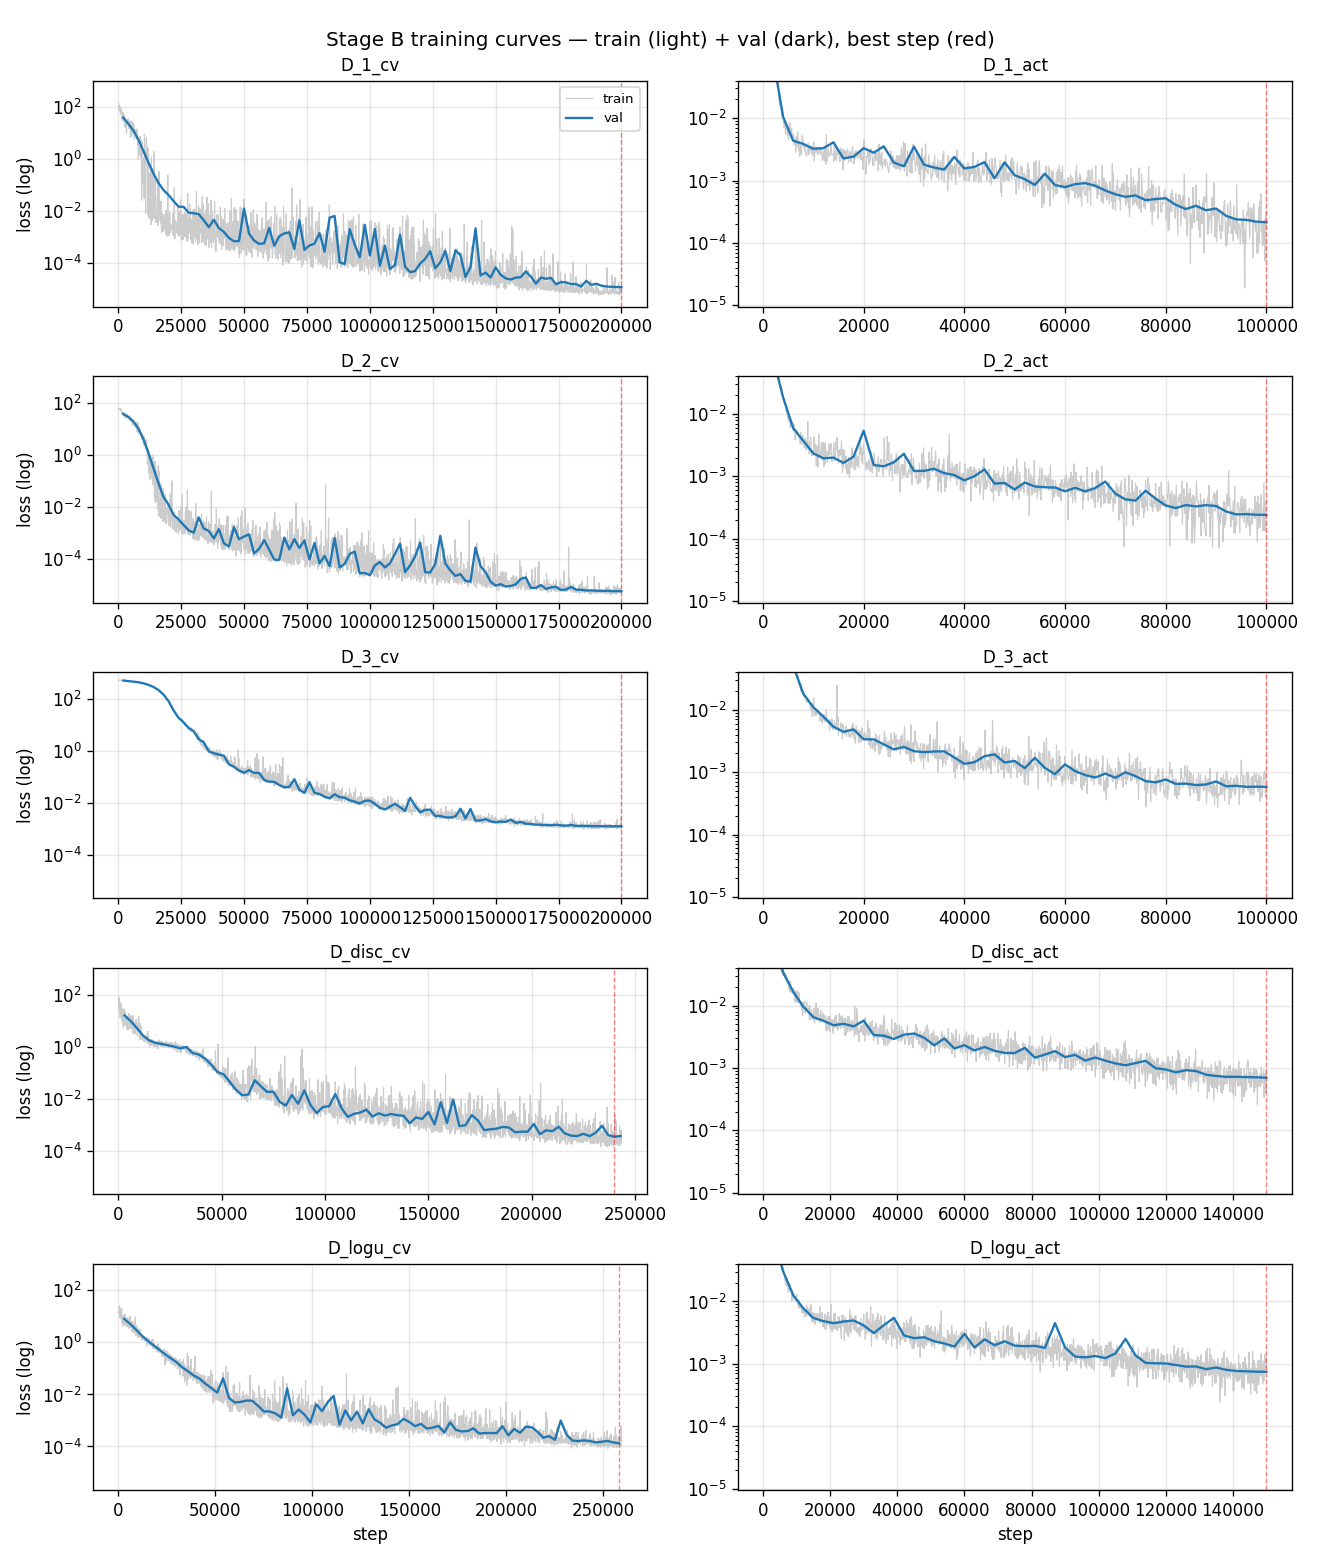
\includegraphics[width=\textwidth]{figures/training-curves.png}
\caption{Train (light) and validation (dark) loss for all ten trained runs, with the best-validation-loss checkpoint step marked (red dashed).}
\label{fig:training-curves}
\end{figure}

For the four random-variance runs we additionally report validation loss separated by $\sigma$-bin (Figure~\ref{fig:training-curves-per-sigma}). On the $\sigma_i^2$-normalized continuation-value runs ($\mathcal{D}_{\mathrm{disc}}$\_cv and $\mathcal{D}_{\mathrm{logu}}$\_cv), the per-$\sigma$ losses are within an order of magnitude of each other for most of training and within $\sim 0.05$ of each other by the end of the $3 \times 10^5$-step budget --- the loss-value-invariance signature targeted by the normalization choice (Section~\ref{sec:training-objective}). The same balance is reported for the action runs.

\begin{figure}[H]
\centering
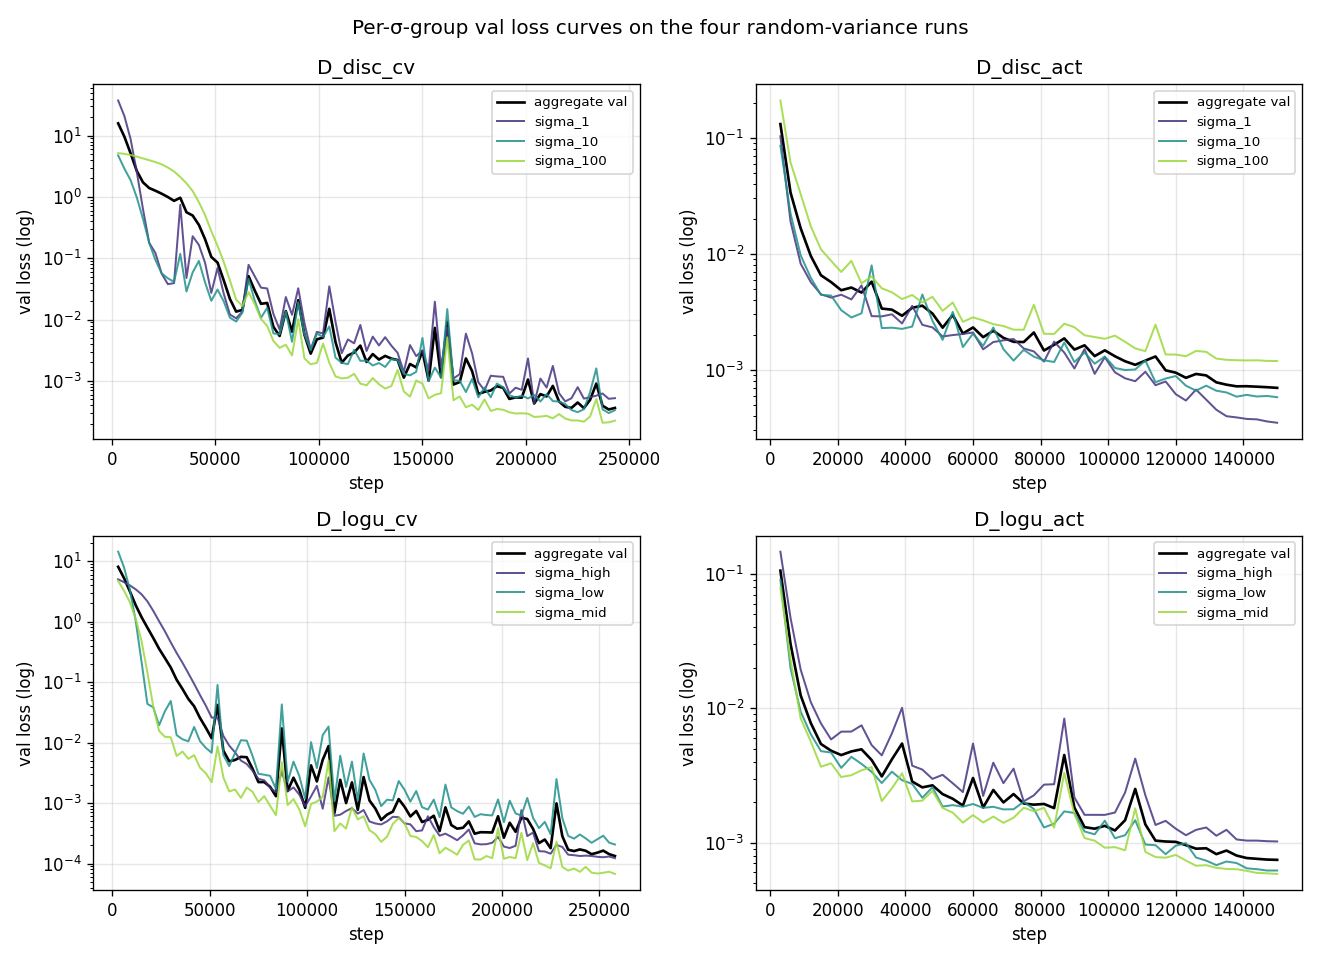
\includegraphics[width=\textwidth]{figures/training-curves-per-sigma.png}
\caption{Per-$\sigma$-bin validation loss for the four random-variance training runs ($\mathcal{D}_{\mathrm{disc}}$\_cv, $\mathcal{D}_{\mathrm{disc}}$\_act, $\mathcal{D}_{\mathrm{logu}}$\_cv, $\mathcal{D}_{\mathrm{logu}}$\_act). Black: aggregate; coloured: per-$\sigma$ slice.}
\label{fig:training-curves-per-sigma}
\end{figure}

\section{Agreement vs.\ payoff: a misleading diagnostic}
\label{sec:res-agreement}

Per-step action agreement and the competitive ratio can differ sharply on the same (model, test regime) cell. The clearest example is $\mathcal{D}_3$\_cv on $\mathcal{D}_1$ (Figure~\ref{fig:agreement-oracle}): the model agrees with the per-regime oracle on $97.8\%$ of decisions yet attains $R/R^\star = 0.016$. The mismatch is mechanical: most timesteps are trivial rejects (the optimal action is ``continue'' and any sufficiently large threshold also rejects), inflating agreement; the few decision-critical timesteps determine the entire payoff. We retain agreement as a diagnostic accompanying $R/R^\star$, never as a substitute for it.

\begin{figure}[H]
\centering
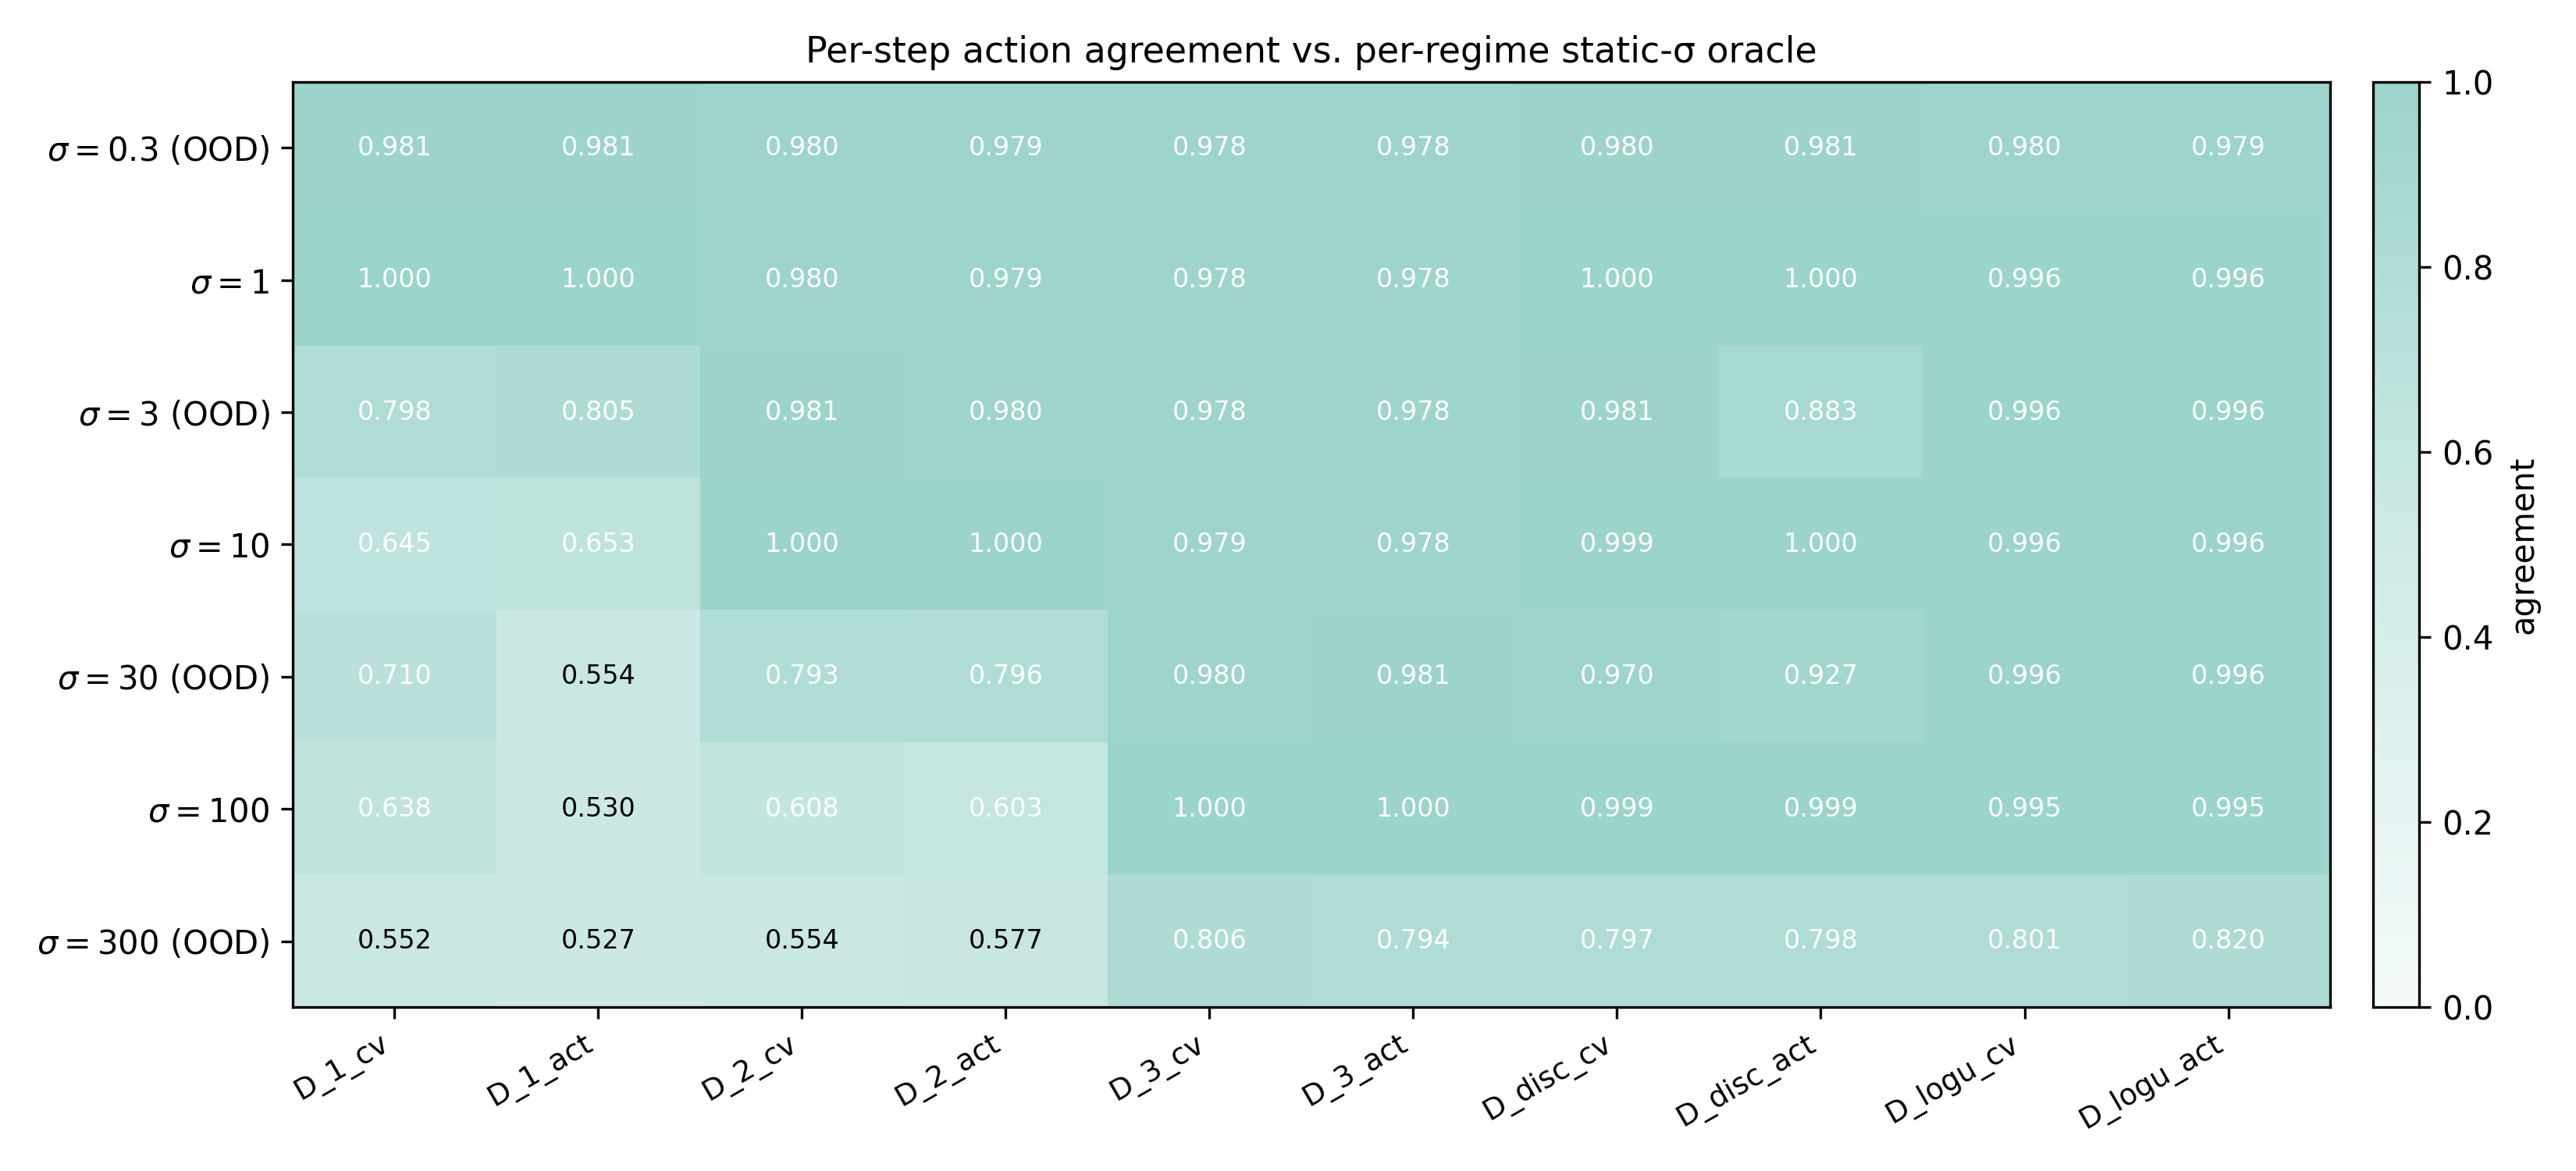
\includegraphics[width=0.85\textwidth]{figures/agreement-oracle.png}
\caption{Per-step action agreement between each trained model (columns) and the per-regime static-$\sigma$ oracle (rows), same axes as Figure~\ref{fig:payoff-and-agreement}.}
\label{fig:agreement-oracle}
\end{figure}

\section{Hindsight (offline-prophet) supervision}
\label{app:offline-supervision}

We replace the ADP-oracle labels of Section~\ref{sec:labeling} with their hindsight counterparts and retrain the four random-variance models. For each sampled $X_{1:n}$, the offline labels are $y_t^{\mathrm{cv}} := \max_{s > t} X_s$ and $y_t^{\mathrm{act}} := \mathbf{1}[X_t \ge \max_{s > t} X_s]$ for $t = 1, \ldots, n-1$, with $y_n^{\mathrm{act}} = 1$ and the continuation-value label at $t = n$ masked out. The labels are computed by a single reverse-cummax pass --- $O(n)$ per sequence, no ADP table. All other hyperparameters match the oracle-supervised counterparts ($\mathcal{D}_{\mathrm{disc}}$\_cv, $\mathcal{D}_{\mathrm{disc}}$\_act, $\mathcal{D}_{\mathrm{logu}}$\_cv, $\mathcal{D}_{\mathrm{logu}}$\_act; the $1/\sigma_i^2$ continuation-value loss normalizer still applies because the prophet value scales with $\sigma$ just like the oracle's). Evaluation uses the same seven static-$\sigma$ test caches and the same $R^\star$ normalizer as Section~\ref{sec:res-ood}.

Mean $R/R^\star$ gap (offline minus oracle) across the seven regimes: $\mathcal{D}_{\mathrm{disc}}$\_cv $-0.059$, $\mathcal{D}_{\mathrm{disc}}$\_act $-0.022$, $\mathcal{D}_{\mathrm{logu}}$\_cv $-0.004$, $\mathcal{D}_{\mathrm{logu}}$\_act $+0.016$. On $\mathcal{D}_{\mathrm{logu}}$ both gaps are within $0.02$ of zero; on $\mathcal{D}_{\mathrm{disc}}$ they are concentrated almost entirely at the $\sigma = 3$ interpolation regime (cv $-0.31$, act $-0.13$), where the oracle-supervised model already exceeds its prior's Bayes-optimal threshold by a $1.6\times$--$2.5\times$ margin (Figure~\ref{fig:per-sigma-disc-extended}) and the hindsight labeler lacks the prior-injected correction that lets the ADP oracle deliver that windfall.

\begin{figure}[H]
\centering
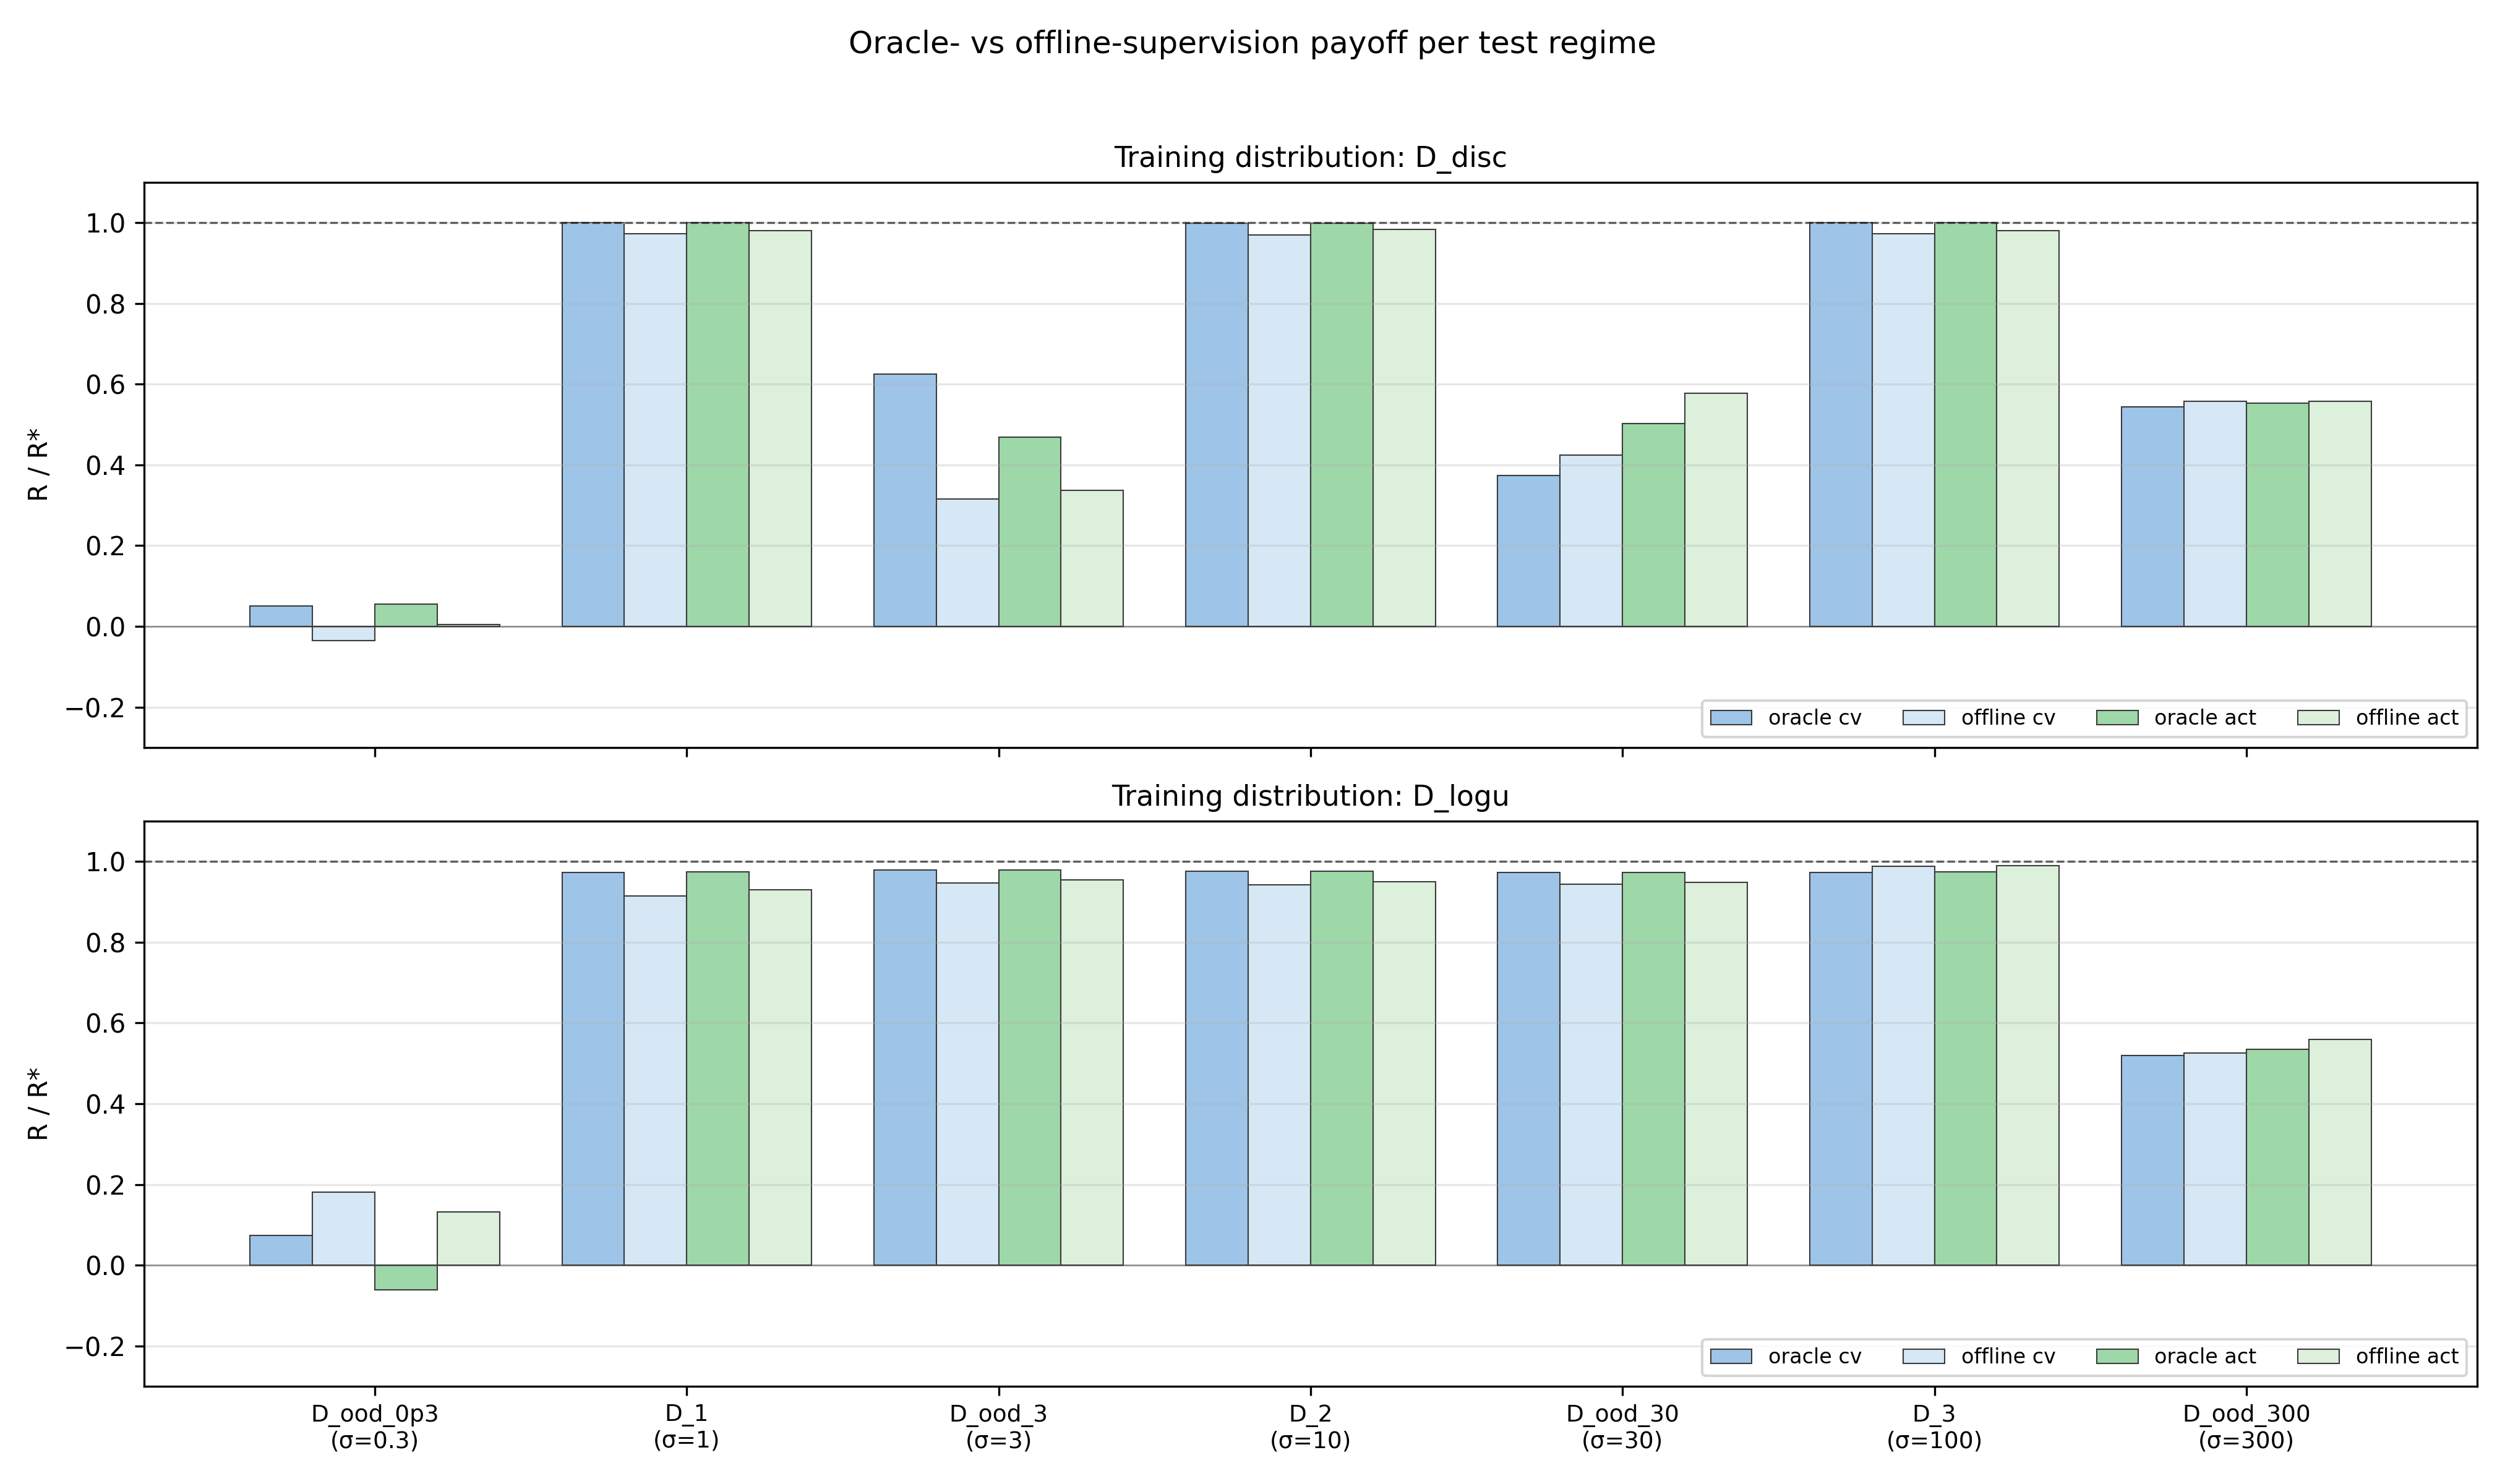
\includegraphics[width=\textwidth]{figures/bars-oracle-vs-offline.png}
\caption{Oracle- vs.\ offline-supervision $R/R^\star$ per test regime, one panel per training distribution. On $\mathcal{D}_{\mathrm{logu}}$ the four bars are visually indistinguishable on every in-prior regime; on $\mathcal{D}_{\mathrm{disc}}$ the offline continuation-value bar dips below its oracle counterpart at $\sigma = 3$.}
\label{fig:offline-bars}
\end{figure}

The offline continuation value is structurally the prophet value --- $y_t^{\mathrm{cv,offline}} \ge C^\star_t$ pointwise --- so the resulting policy accepts less often than the oracle's. Figures~\ref{fig:offline-traj-disc} and \ref{fig:offline-traj-logu} show this directly: the offline continuation-value threshold sits visibly above its oracle counterpart on every in-prior regime. The conservatism is benign on the Gaussian--Gaussian model used here because Gaussian tails decay fast enough that the right-tail mass a prophet rule waits for is reliably present in each sequence; over-waiting costs at most a small predictable margin rather than a structural failure to stop --- below $0.02$ in $R/R^\star$ on every regime except $\mathcal{D}_{\mathrm{disc}}$\_$\sigma{=}3$. On a generative model with heavier tails or rarer right-tail events the same construction would not necessarily be benign.

\begin{figure}[H]
\centering
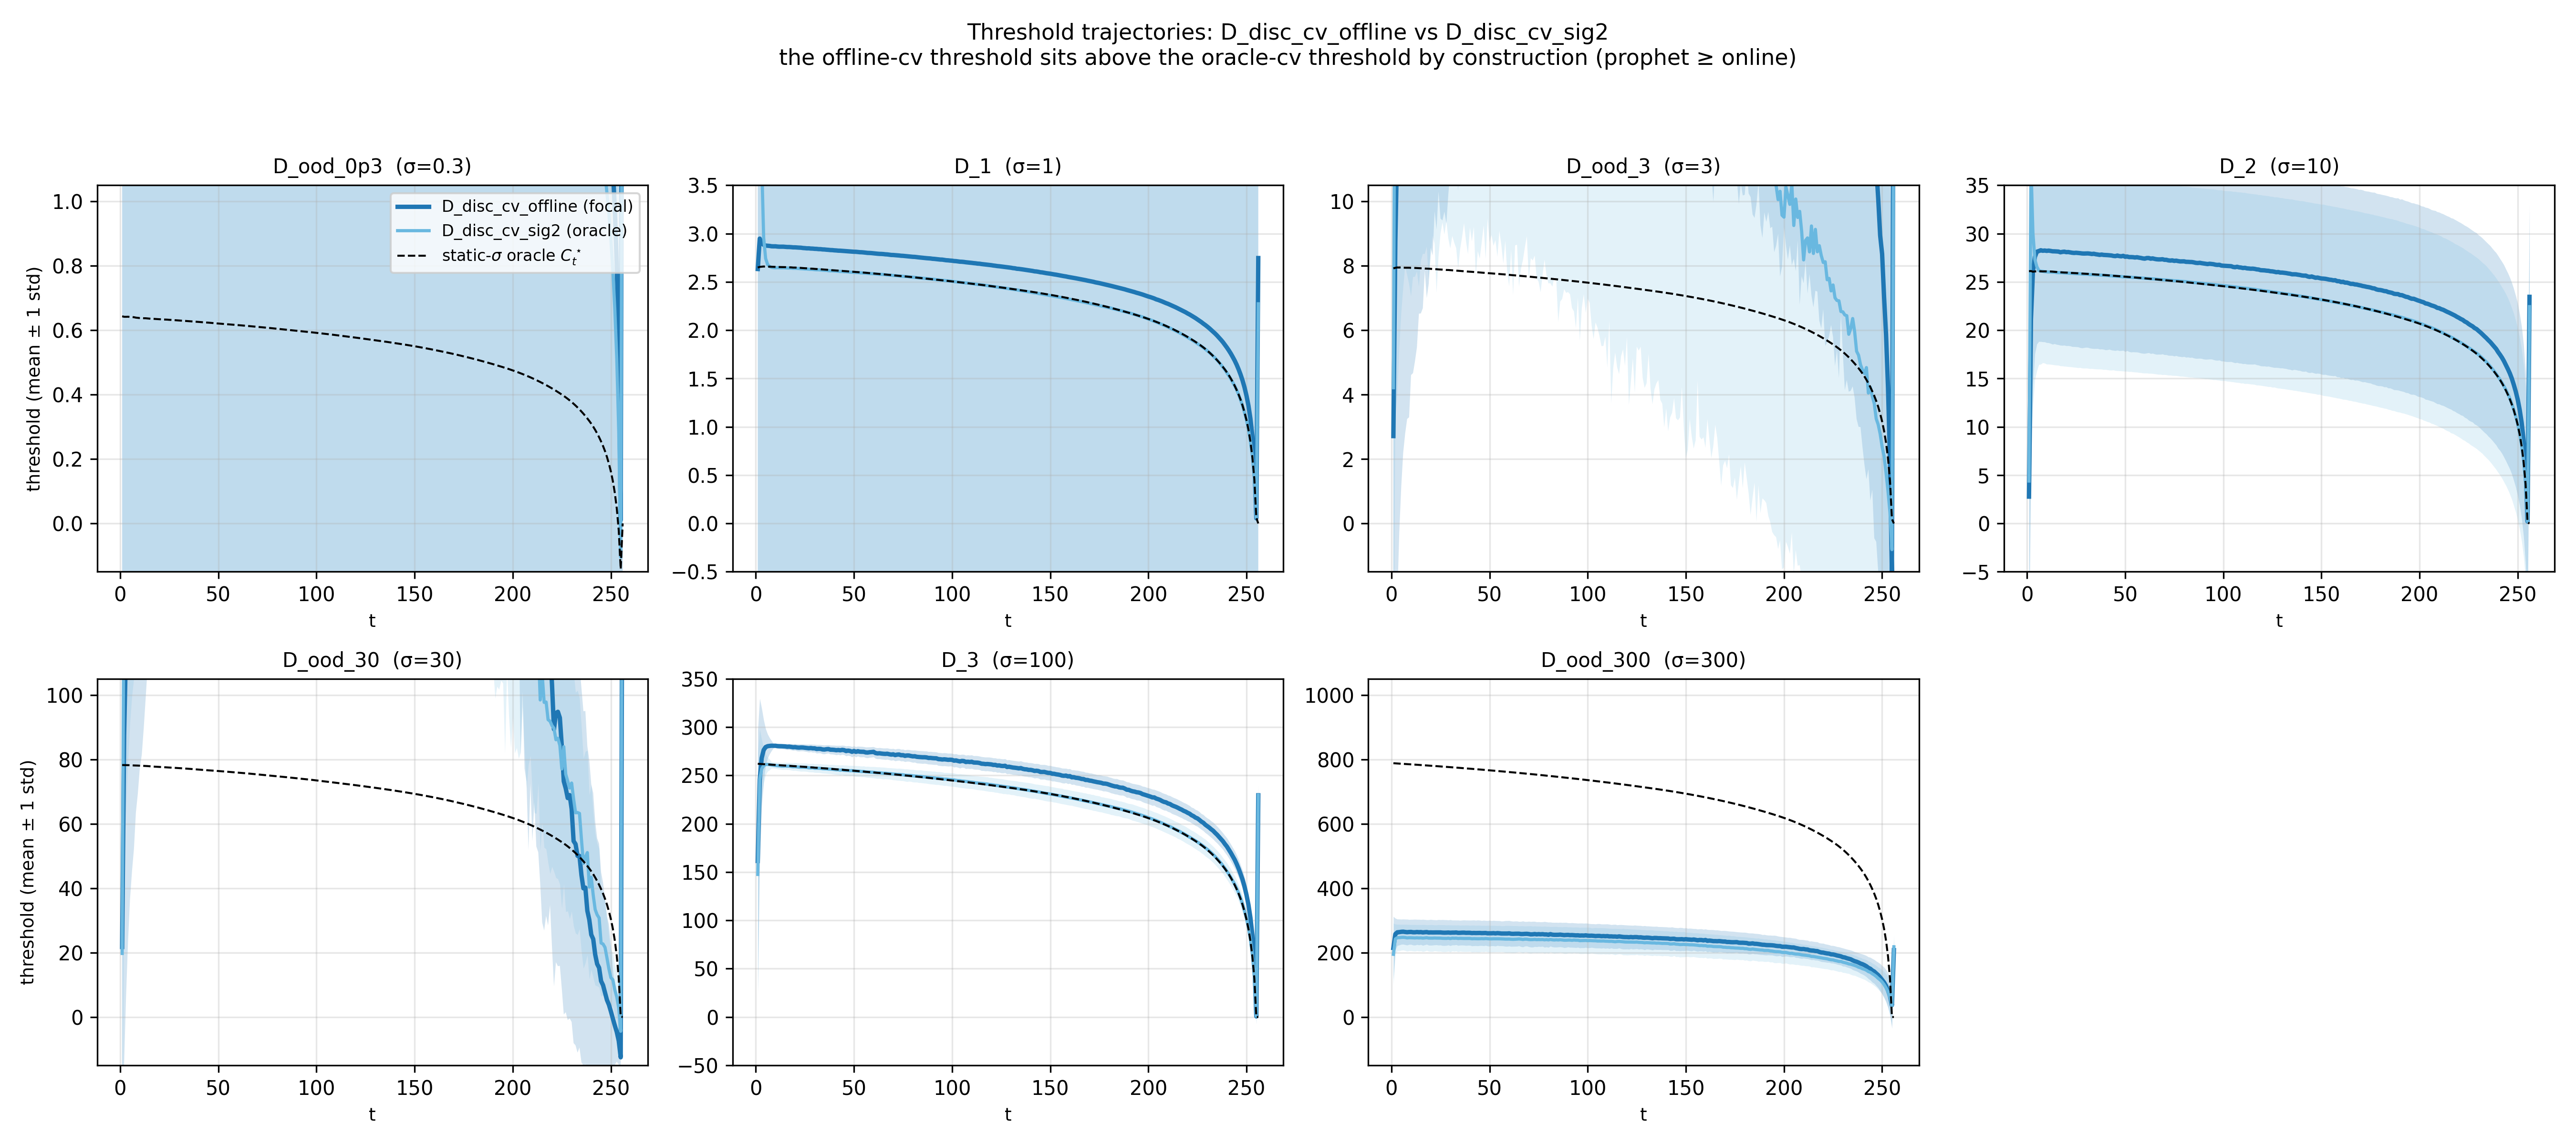
\includegraphics[width=\textwidth]{figures/trajectories-d-disc-cv-offline.png}
\caption{Threshold trajectories for $\mathcal{D}_{\mathrm{disc}}$\_cv\_offline (focal, blue, $\pm 1$ std band), the oracle counterpart $\mathcal{D}_{\mathrm{disc}}$\_cv (pale blue), and the per-regime static-$\sigma$ oracle $C^\star_t$ (black dashed) on all seven test regimes. The offline threshold sits above the oracle threshold by construction (prophet $\ge$ online).}
\label{fig:offline-traj-disc}
\end{figure}

\begin{figure}[H]
\centering
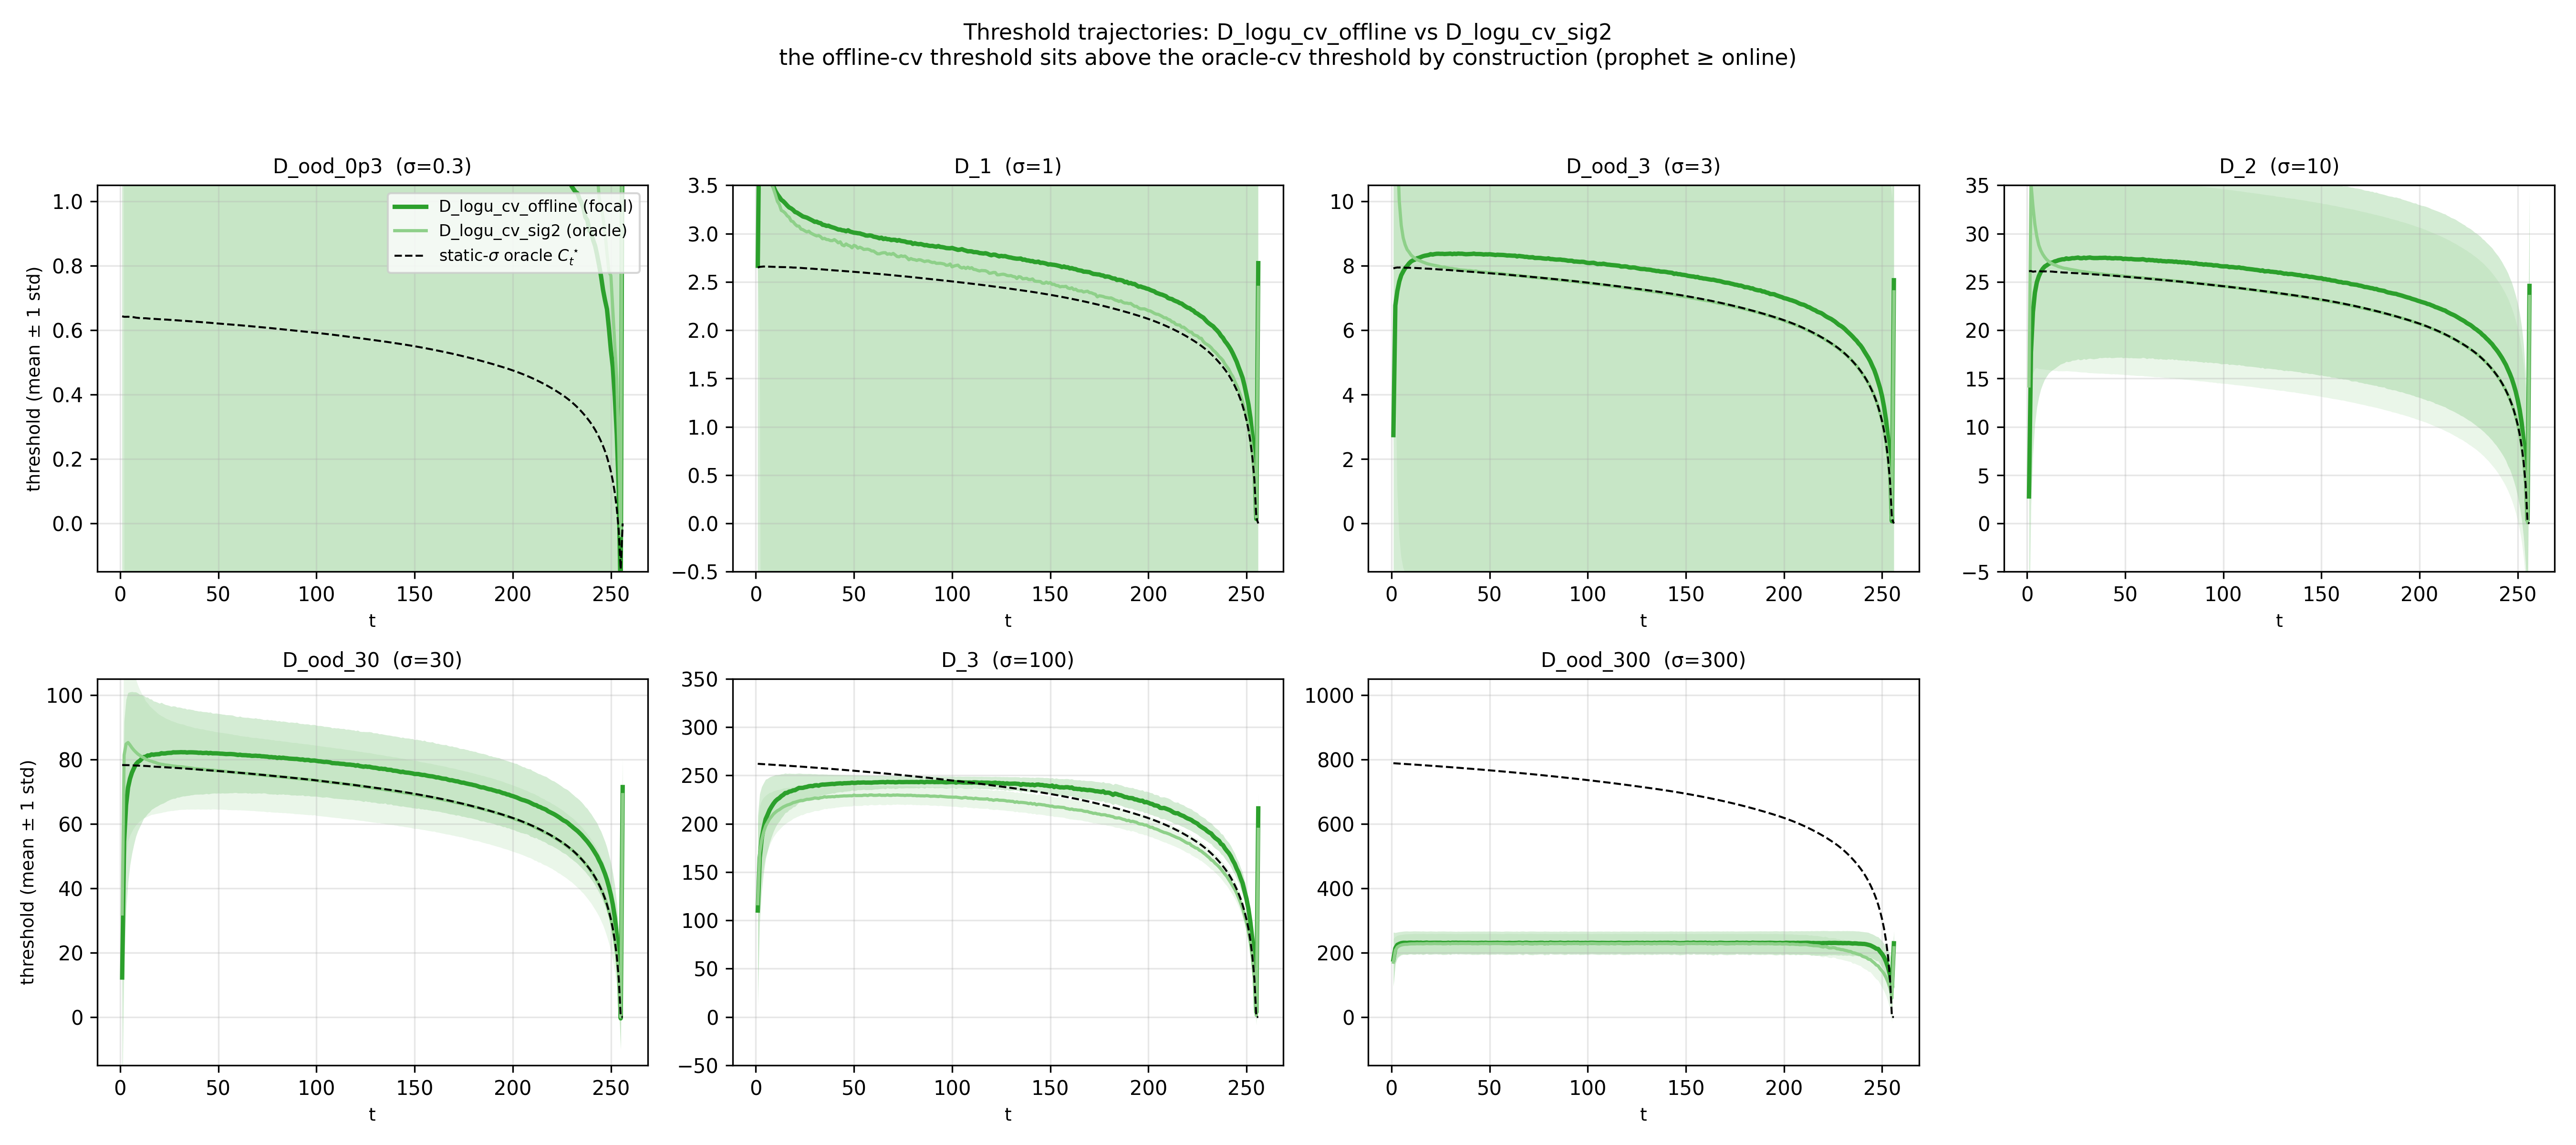
\includegraphics[width=\textwidth]{figures/trajectories-d-logu-cv-offline.png}
\caption{Same layout, focal $\mathcal{D}_{\mathrm{logu}}$\_cv\_offline (green). On $\mathcal{D}_{\mathrm{logu}}$ the offline threshold tracks both the oracle's threshold and $C^\star_t$ closely on every regime.}
\label{fig:offline-traj-logu}
\end{figure}

\section{Temporal shift: detailed statistics}
\label{app:regime-shift-stats}

This appendix collects the per-shift summary statistics and per-sequence $t_{1/2}$ histograms summarised in Section~\ref{sec:res-shift}.

\begin{table}[H]
\centering
\scriptsize
\begin{tabular}{llrrrrrrrrr}
\hline
set & model & shift & mean $t_{1/2}$ & $p_{10}$ & $p_{50}$ & $p_{90}$ & never & pre err & post err & $\rho_{200}$ \\
\hline
B.1 & $\mathcal{D}_{\mathrm{disc}}$\_cv & $\sigma{=}1 \to 100$  &   1.8 &   1 &   1 &   3 &    0 &   0.007 &  17.866 & $+0.999$ \\
B.1 & $\mathcal{D}_{\mathrm{logu}}$\_cv & $\sigma{=}1 \to 100$  &   3.2 &   1 &   3 &   6 &    0 &   0.186 &  45.075 & $+0.910$ \\
B.1 & $\mathcal{D}_{\mathrm{disc}}$\_cv & $\sigma{=}100 \to 1$  & 127.0 & 127 & 127 & 127 &   13 &   0.953 & 167.554 & $-0.010$ \\
B.1 & $\mathcal{D}_{\mathrm{logu}}$\_cv & $\sigma{=}100 \to 1$  & 127.0 & 127 & 127 & 127 &   16 &  19.148 & 117.001 & $+0.050$ \\
B.1 & $\mathcal{D}_{\mathrm{disc}}$\_cv & $\sigma{=}10 \to 100$ &   2.9 &   1 &   2 &   6 &    0 &   0.085 &  10.529 & $+0.995$ \\
B.1 & $\mathcal{D}_{\mathrm{logu}}$\_cv & $\sigma{=}10 \to 100$ &  16.1 &   8 &  15 &  25 &    0 &   1.531 &  52.451 & $+0.798$ \\
B.1 & $\mathcal{D}_{\mathrm{disc}}$\_cv & $\sigma{=}100 \to 10$ & 126.9 & 127 & 127 & 127 &   23 &   0.956 & 147.938 & $-0.011$ \\
B.1 & $\mathcal{D}_{\mathrm{logu}}$\_cv & $\sigma{=}100 \to 10$ & 126.8 & 126 & 127 & 127 &   42 &  19.079 & 103.452 & $+0.098$ \\
B.2 & $\mathcal{D}_{\mathrm{disc}}$\_cv & $\sigma{=}3 \to 30$   &  22.5 &   1 &   6 &  69 &    0 &  10.045 &  27.315 & $+0.787$ \\
B.2 & $\mathcal{D}_{\mathrm{logu}}$\_cv & $\sigma{=}3 \to 30$   &  19.2 &   2 &  13 &  40 &    0 &   0.462 &  15.730 & $+0.796$ \\
B.2 & $\mathcal{D}_{\mathrm{disc}}$\_cv & $\sigma{=}30 \to 3$   & 118.8 &  99 & 128 & 128 & 5502 & 157.042 &  38.454 & $-0.162$ \\
B.2 & $\mathcal{D}_{\mathrm{logu}}$\_cv & $\sigma{=}30 \to 3$   & 125.7 & 121 & 128 & 128 & 6773 &   4.618 &  32.137 & $+0.096$ \\
B.2 & $\mathcal{D}_{\mathrm{disc}}$\_cv & $\sigma{=}3 \to 300$  &   1.6 &   1 &   1 &   3 &    0 &  10.040 & 331.656 & $+0.751$ \\
B.2 & $\mathcal{D}_{\mathrm{logu}}$\_cv & $\sigma{=}3 \to 300$  &   4.7 &   1 &   5 &   8 &    0 &   0.466 & 321.764 & $+0.744$ \\
B.2 & $\mathcal{D}_{\mathrm{disc}}$\_cv & $\sigma{=}300 \to 3$  & 126.4 & 125 & 127 & 127 &    2 & 503.619 & 148.685 & $+0.234$ \\
B.2 & $\mathcal{D}_{\mathrm{logu}}$\_cv & $\sigma{=}300 \to 3$  & 126.3 & 124 & 127 & 127 &    2 & 513.776 & 141.471 & $+0.226$ \\
B.2 & $\mathcal{D}_{\mathrm{disc}}$\_cv & $\sigma{=}30 \to 300$ &   2.3 &   1 &   2 &   4 &    0 & 157.246 & 328.141 & $+0.514$ \\
B.2 & $\mathcal{D}_{\mathrm{logu}}$\_cv & $\sigma{=}30 \to 300$ &  39.7 &  29 &  39 &  52 &    0 &   4.611 & 311.692 & $+0.521$ \\
B.2 & $\mathcal{D}_{\mathrm{disc}}$\_cv & $\sigma{=}300 \to 30$ &  51.0 &   3 &  50 & 103 &    0 & 503.605 & 101.728 & $+0.489$ \\
B.2 & $\mathcal{D}_{\mathrm{logu}}$\_cv & $\sigma{=}300 \to 30$ & 100.9 &  89 & 102 & 113 &    0 & 513.787 & 107.438 & $+0.451$ \\
\hline
\end{tabular}
\caption{Per-sequence regime shift (B.1 + B.2), statistics over $N_{\mathrm{test}} = 10^4$ sequences. ``Never'' $=$ sequences whose $\rho_t$ did not cross $0.5$ in the post-shift window. Pre/post err: mean $|\widehat C_t - C^\star_{\sigma, t}|$ over $t \in [50, 128]$ and $[200, 255]$. $\rho_{200}$: population-mean adaptation at $t = 200$.}
\label{tab:res-shift-summary}
\end{table}

\begin{figure}[H]
\centering
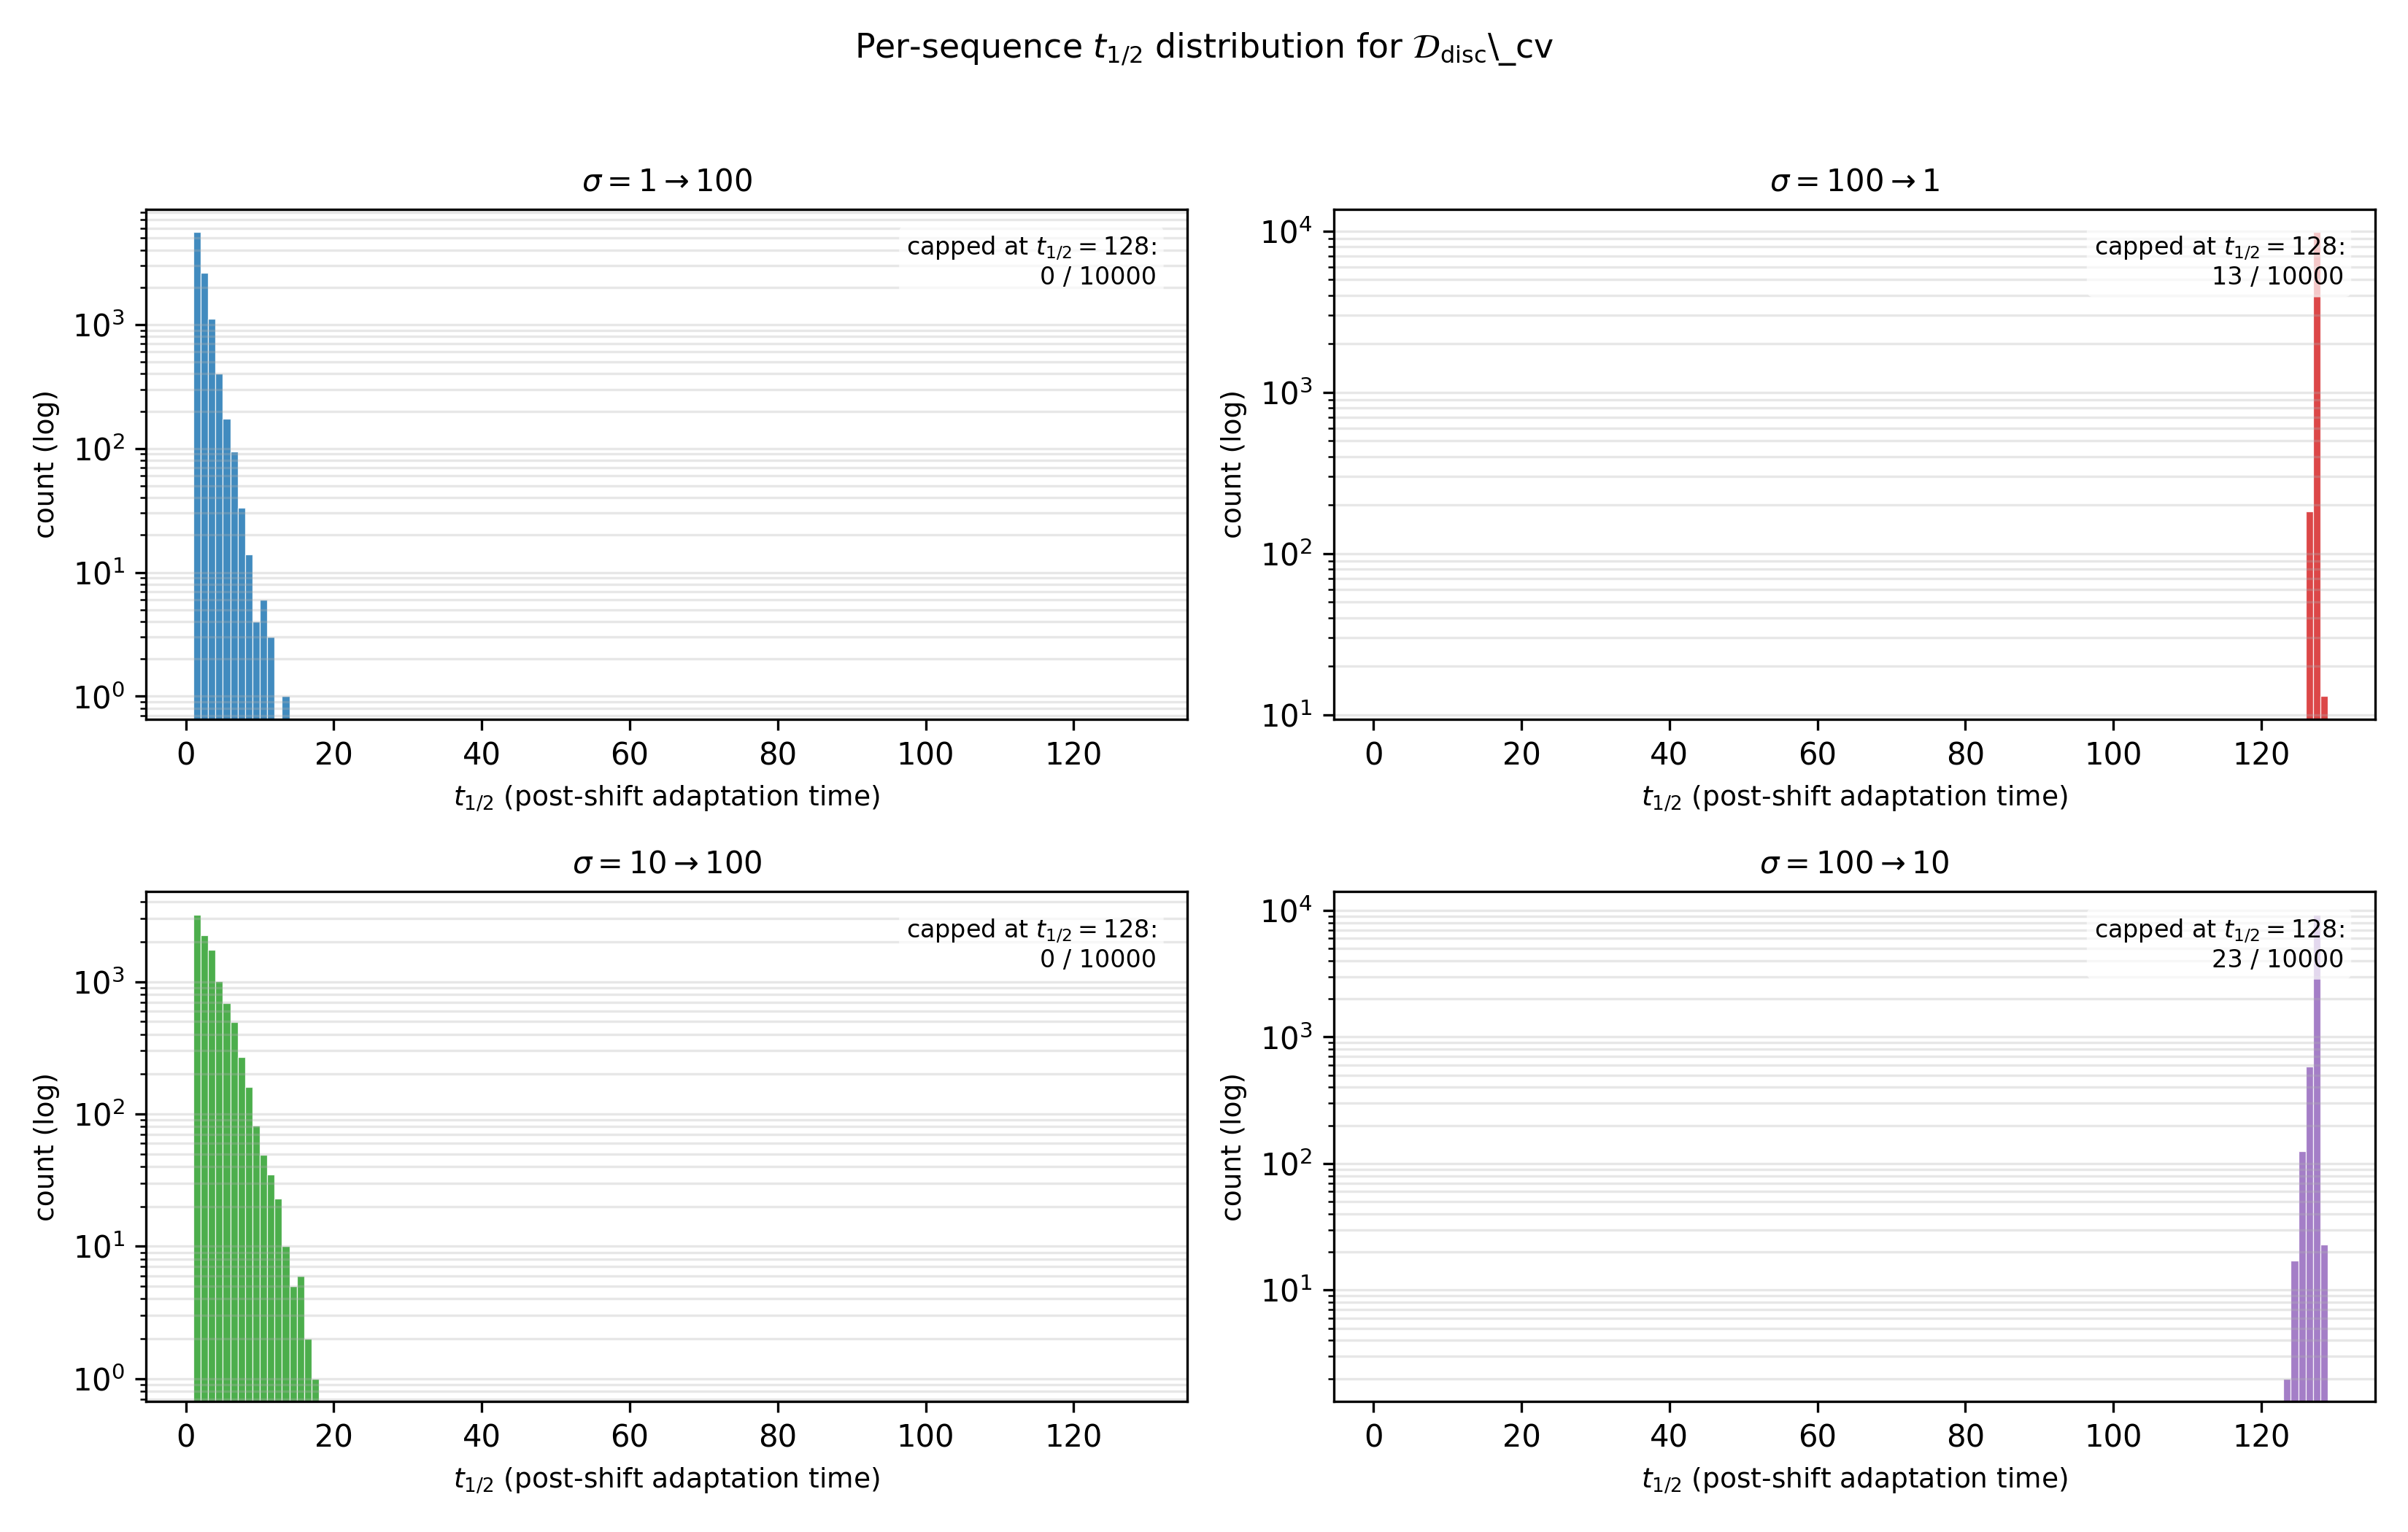
\includegraphics[width=0.7\textwidth]{figures/t_half-hist-D_disc_cv.png}
\caption{Per-sequence $t_{1/2}$ distributions for $\mathcal{D}_{\mathrm{disc}}$\_cv on the four B.1 pairs.}
\label{fig:t-half-hist-disc}
\end{figure}

\begin{figure}[H]
\centering
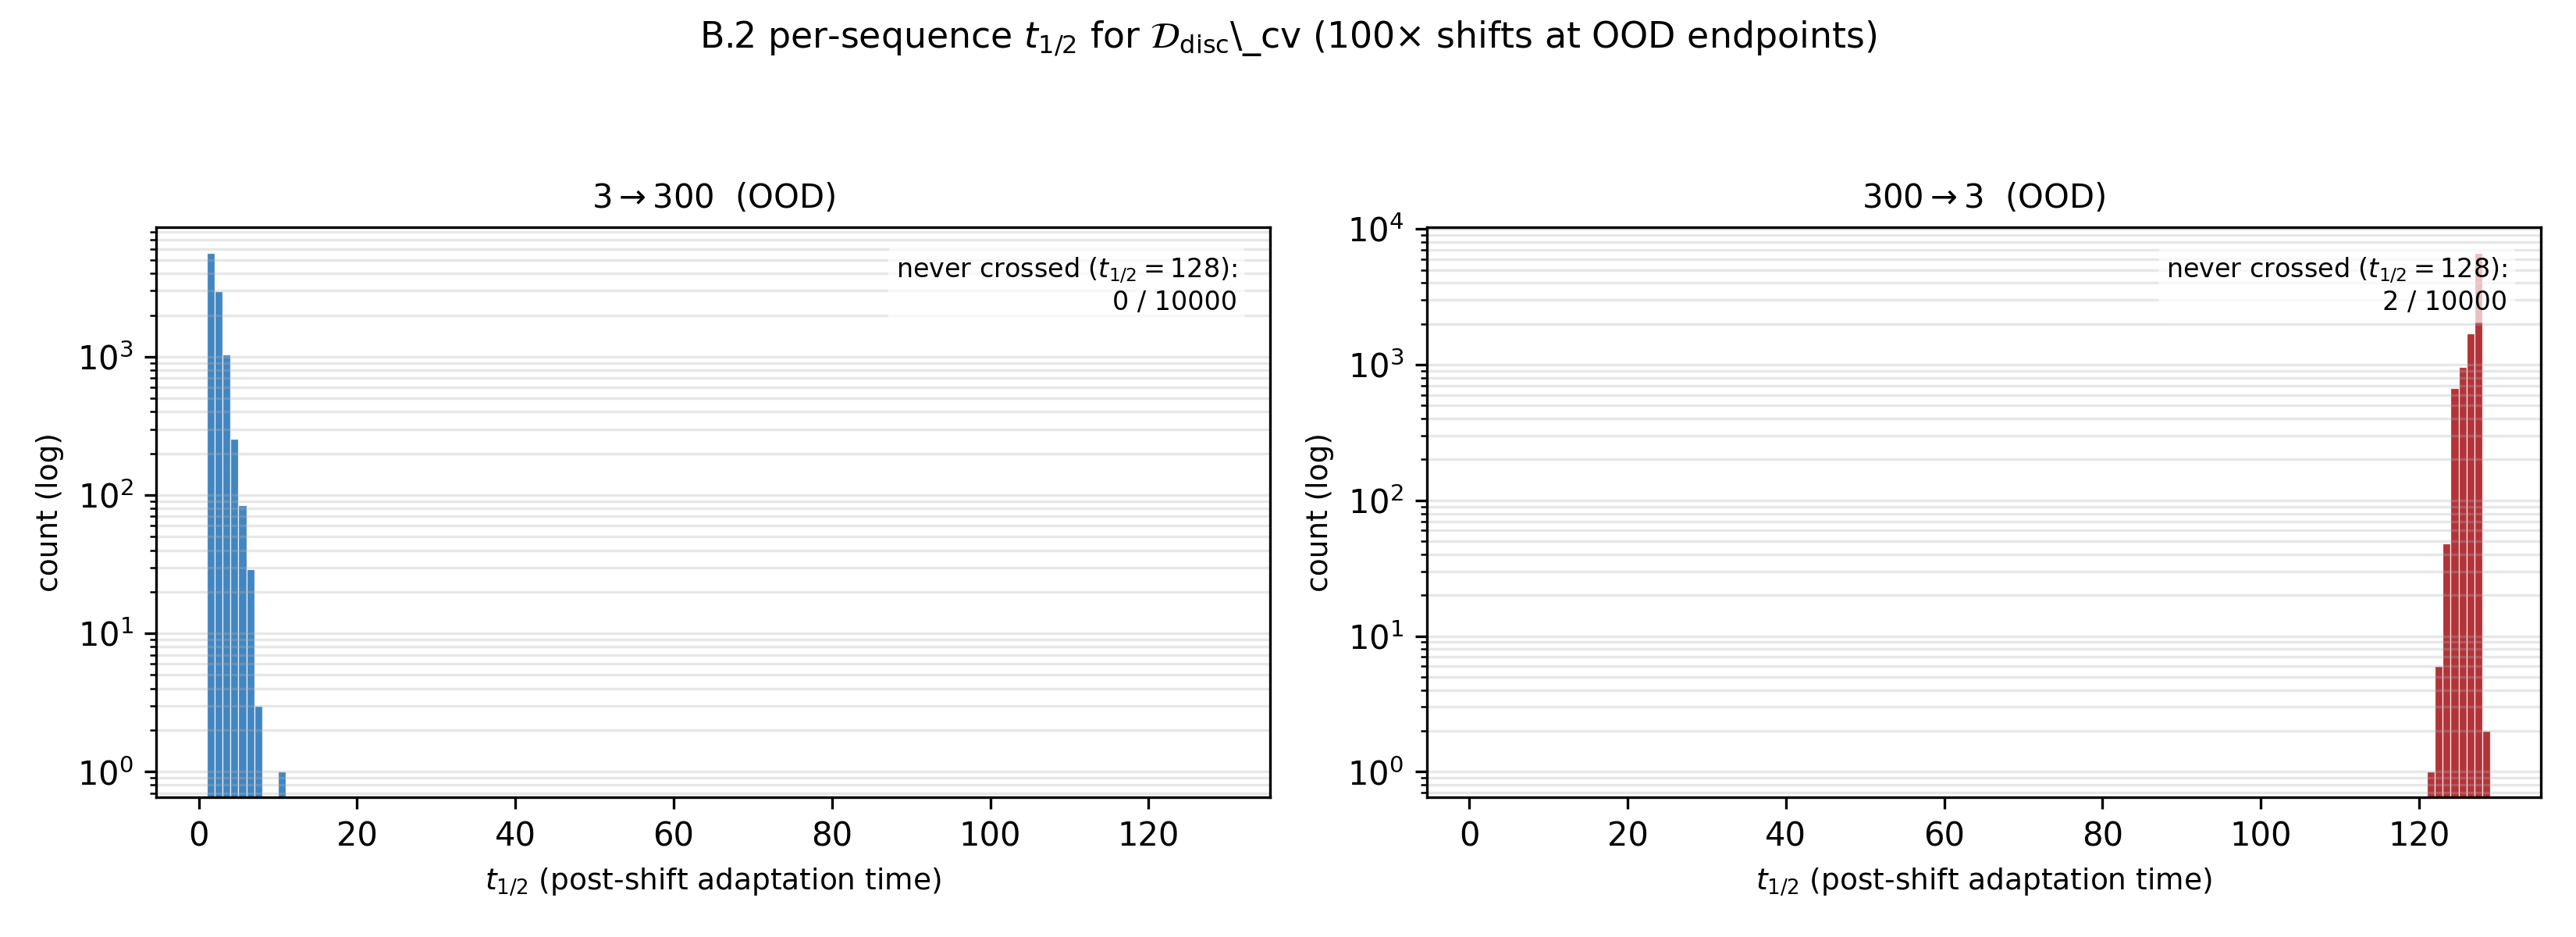
\includegraphics[width=0.7\textwidth]{figures/t_half-hist-b2-D_disc_cv.png}
\caption{Per-sequence $t_{1/2}$ distributions for $\mathcal{D}_{\mathrm{disc}}$\_cv on the two B.2 $100\times$ pairs.}
\label{fig:t-half-hist-b2-disc}
\end{figure}

\section{Single-shot probing results}
\label{sec:probe-results}

This appendix collects the single-shot probe curves for the two random-variance models (per-timestep and attention-pooled probe variants, plus a cross-distribution overlay). These are descriptive results from a single training run per model; the planned paired-ensemble permutation test of Section~\ref{sec:probe-ensemble} replaces them with statistically grounded estimates.

\begin{figure}[H]
\centering
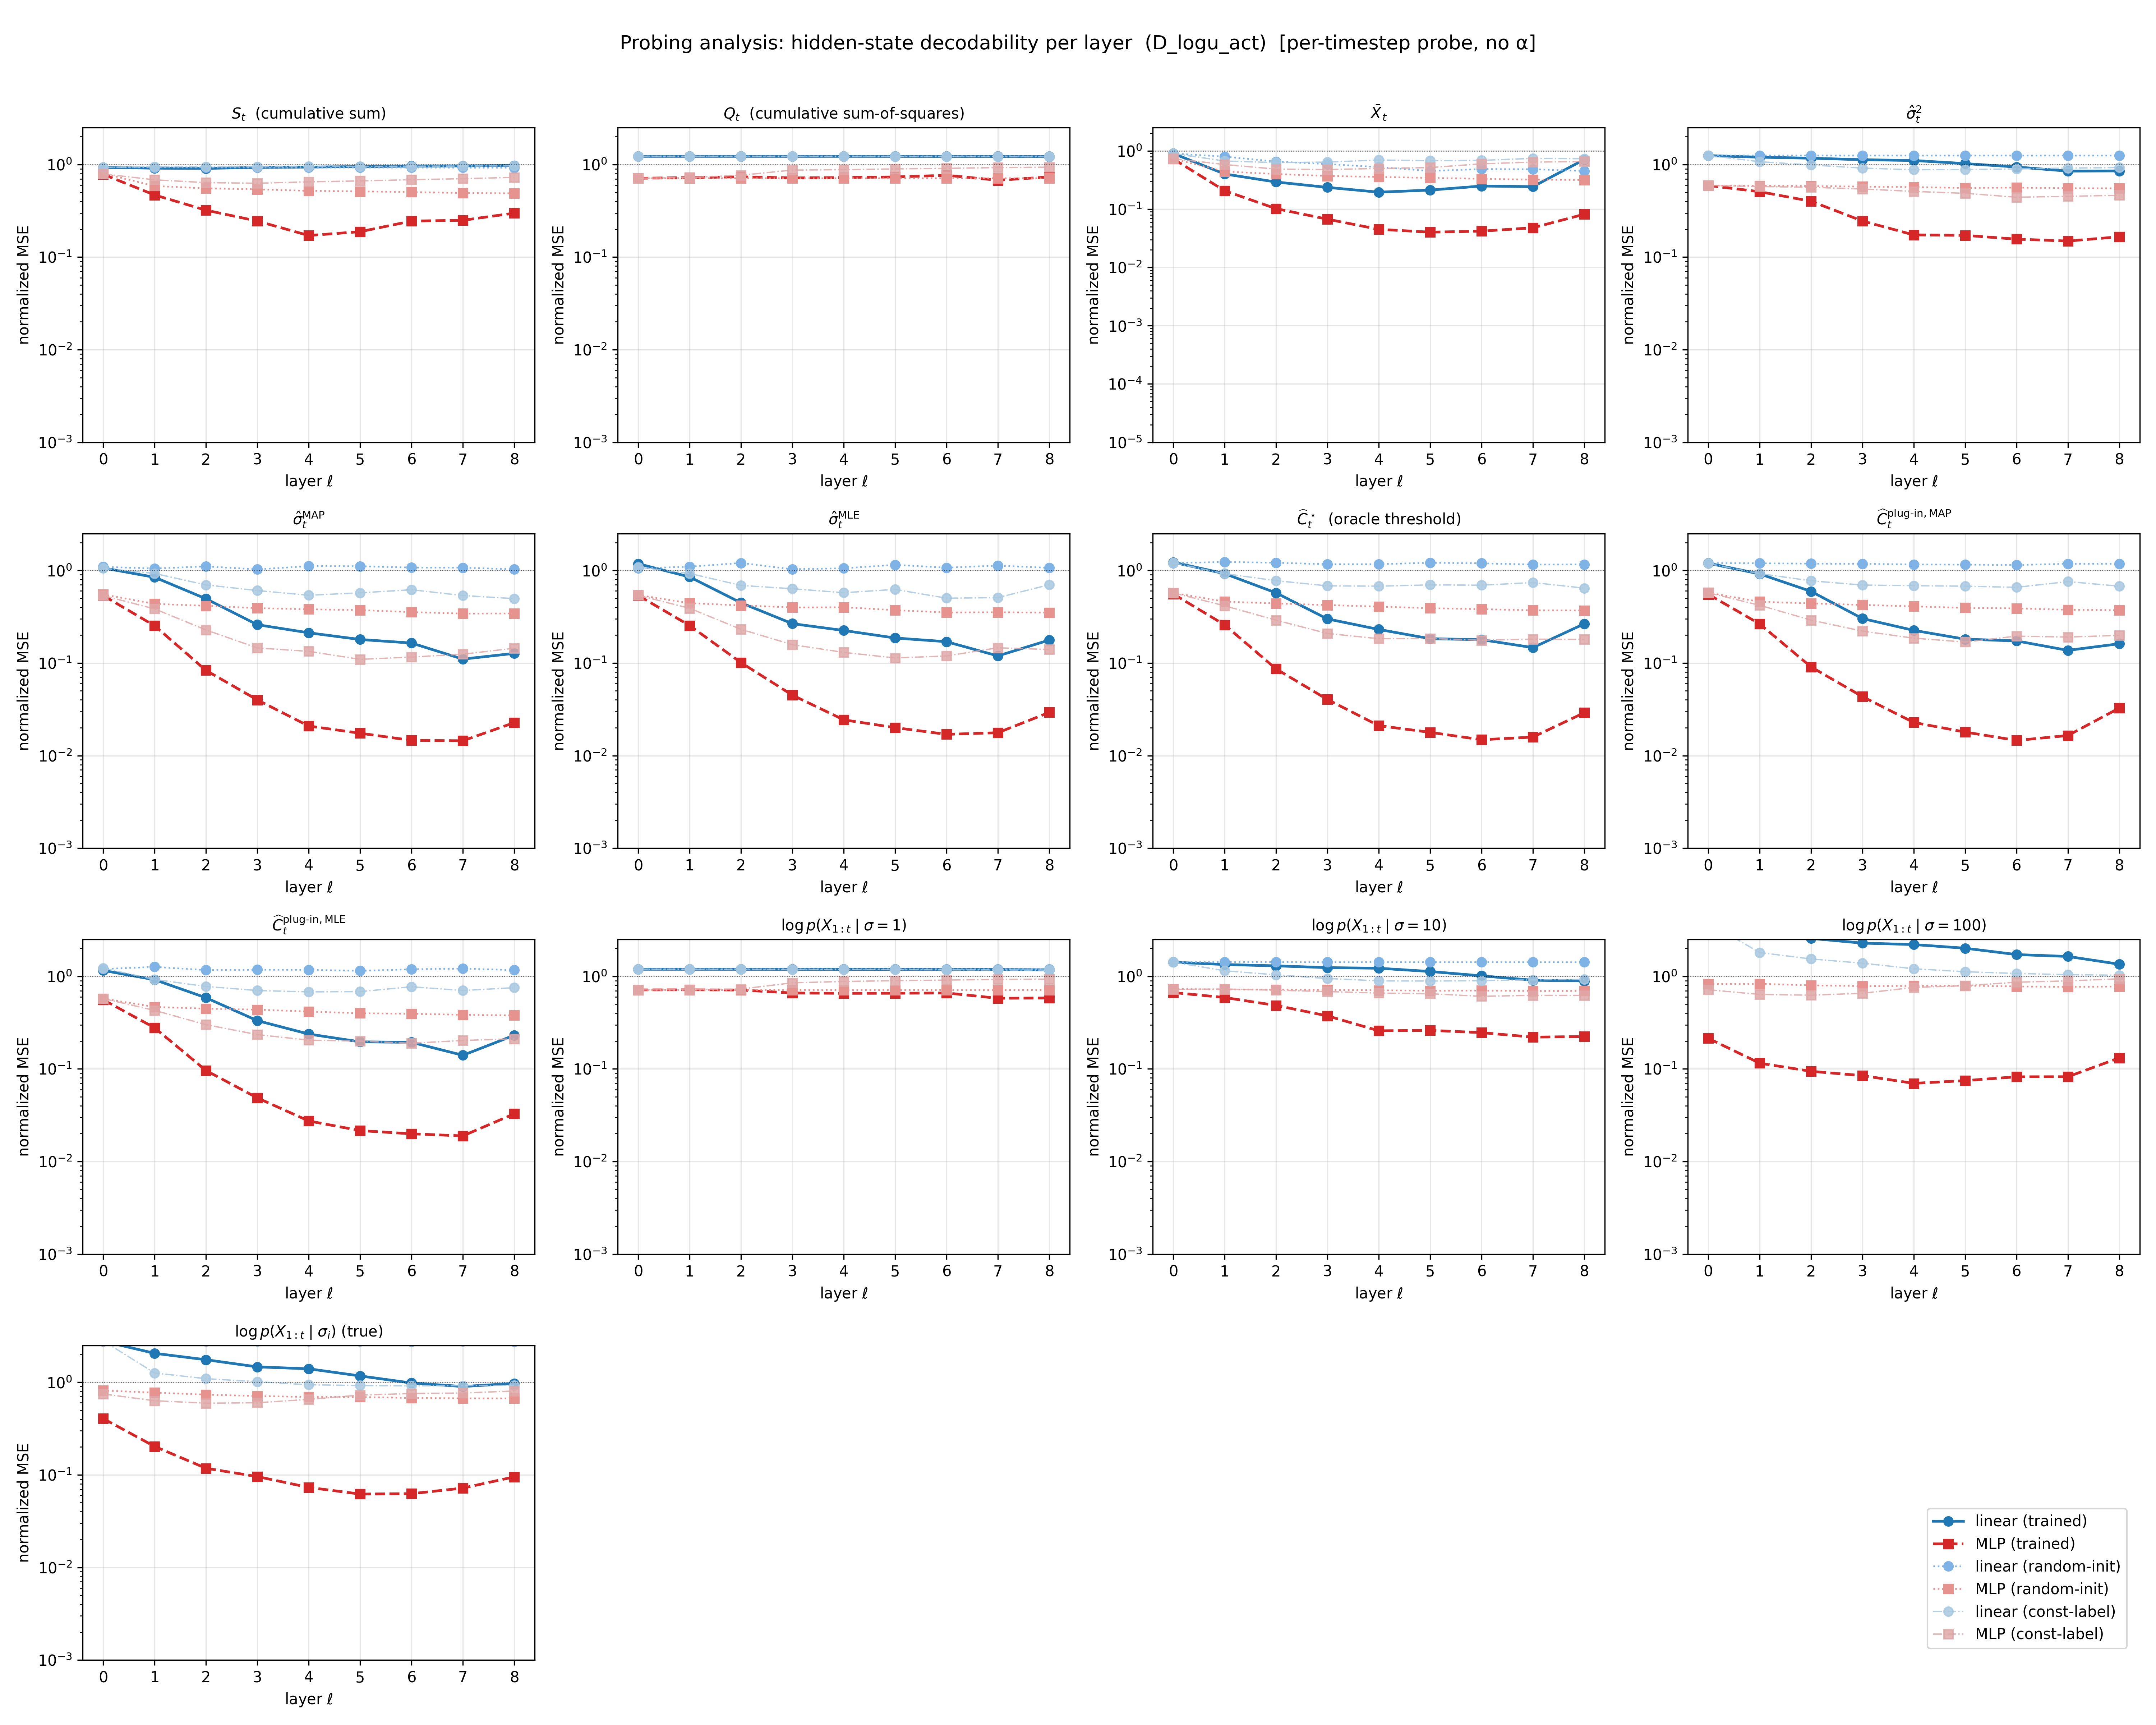
\includegraphics[width=\textwidth]{figures/probe-curves-logu-act-noattn.png}
\caption{$\mathcal{D}_{\mathrm{logu}}$\_act probing, all $13$ targets. Normalized test MSE vs.\ layer $\ell \in \{0, \ldots, 8\}$. Trained: linear probe solid blue, MLP probe (hidden width $512$, GeLU) dashed red. Random-init noise floor: dotted pale blue / pale red. Constant-label control: dot-dashed, lighter. $\mathrm{nMSE} = 1$ (dotted horizontal) is the constant-mean baseline.}
\label{fig:probe-curves-logu-act}
\end{figure}

\begin{figure}[H]
\centering
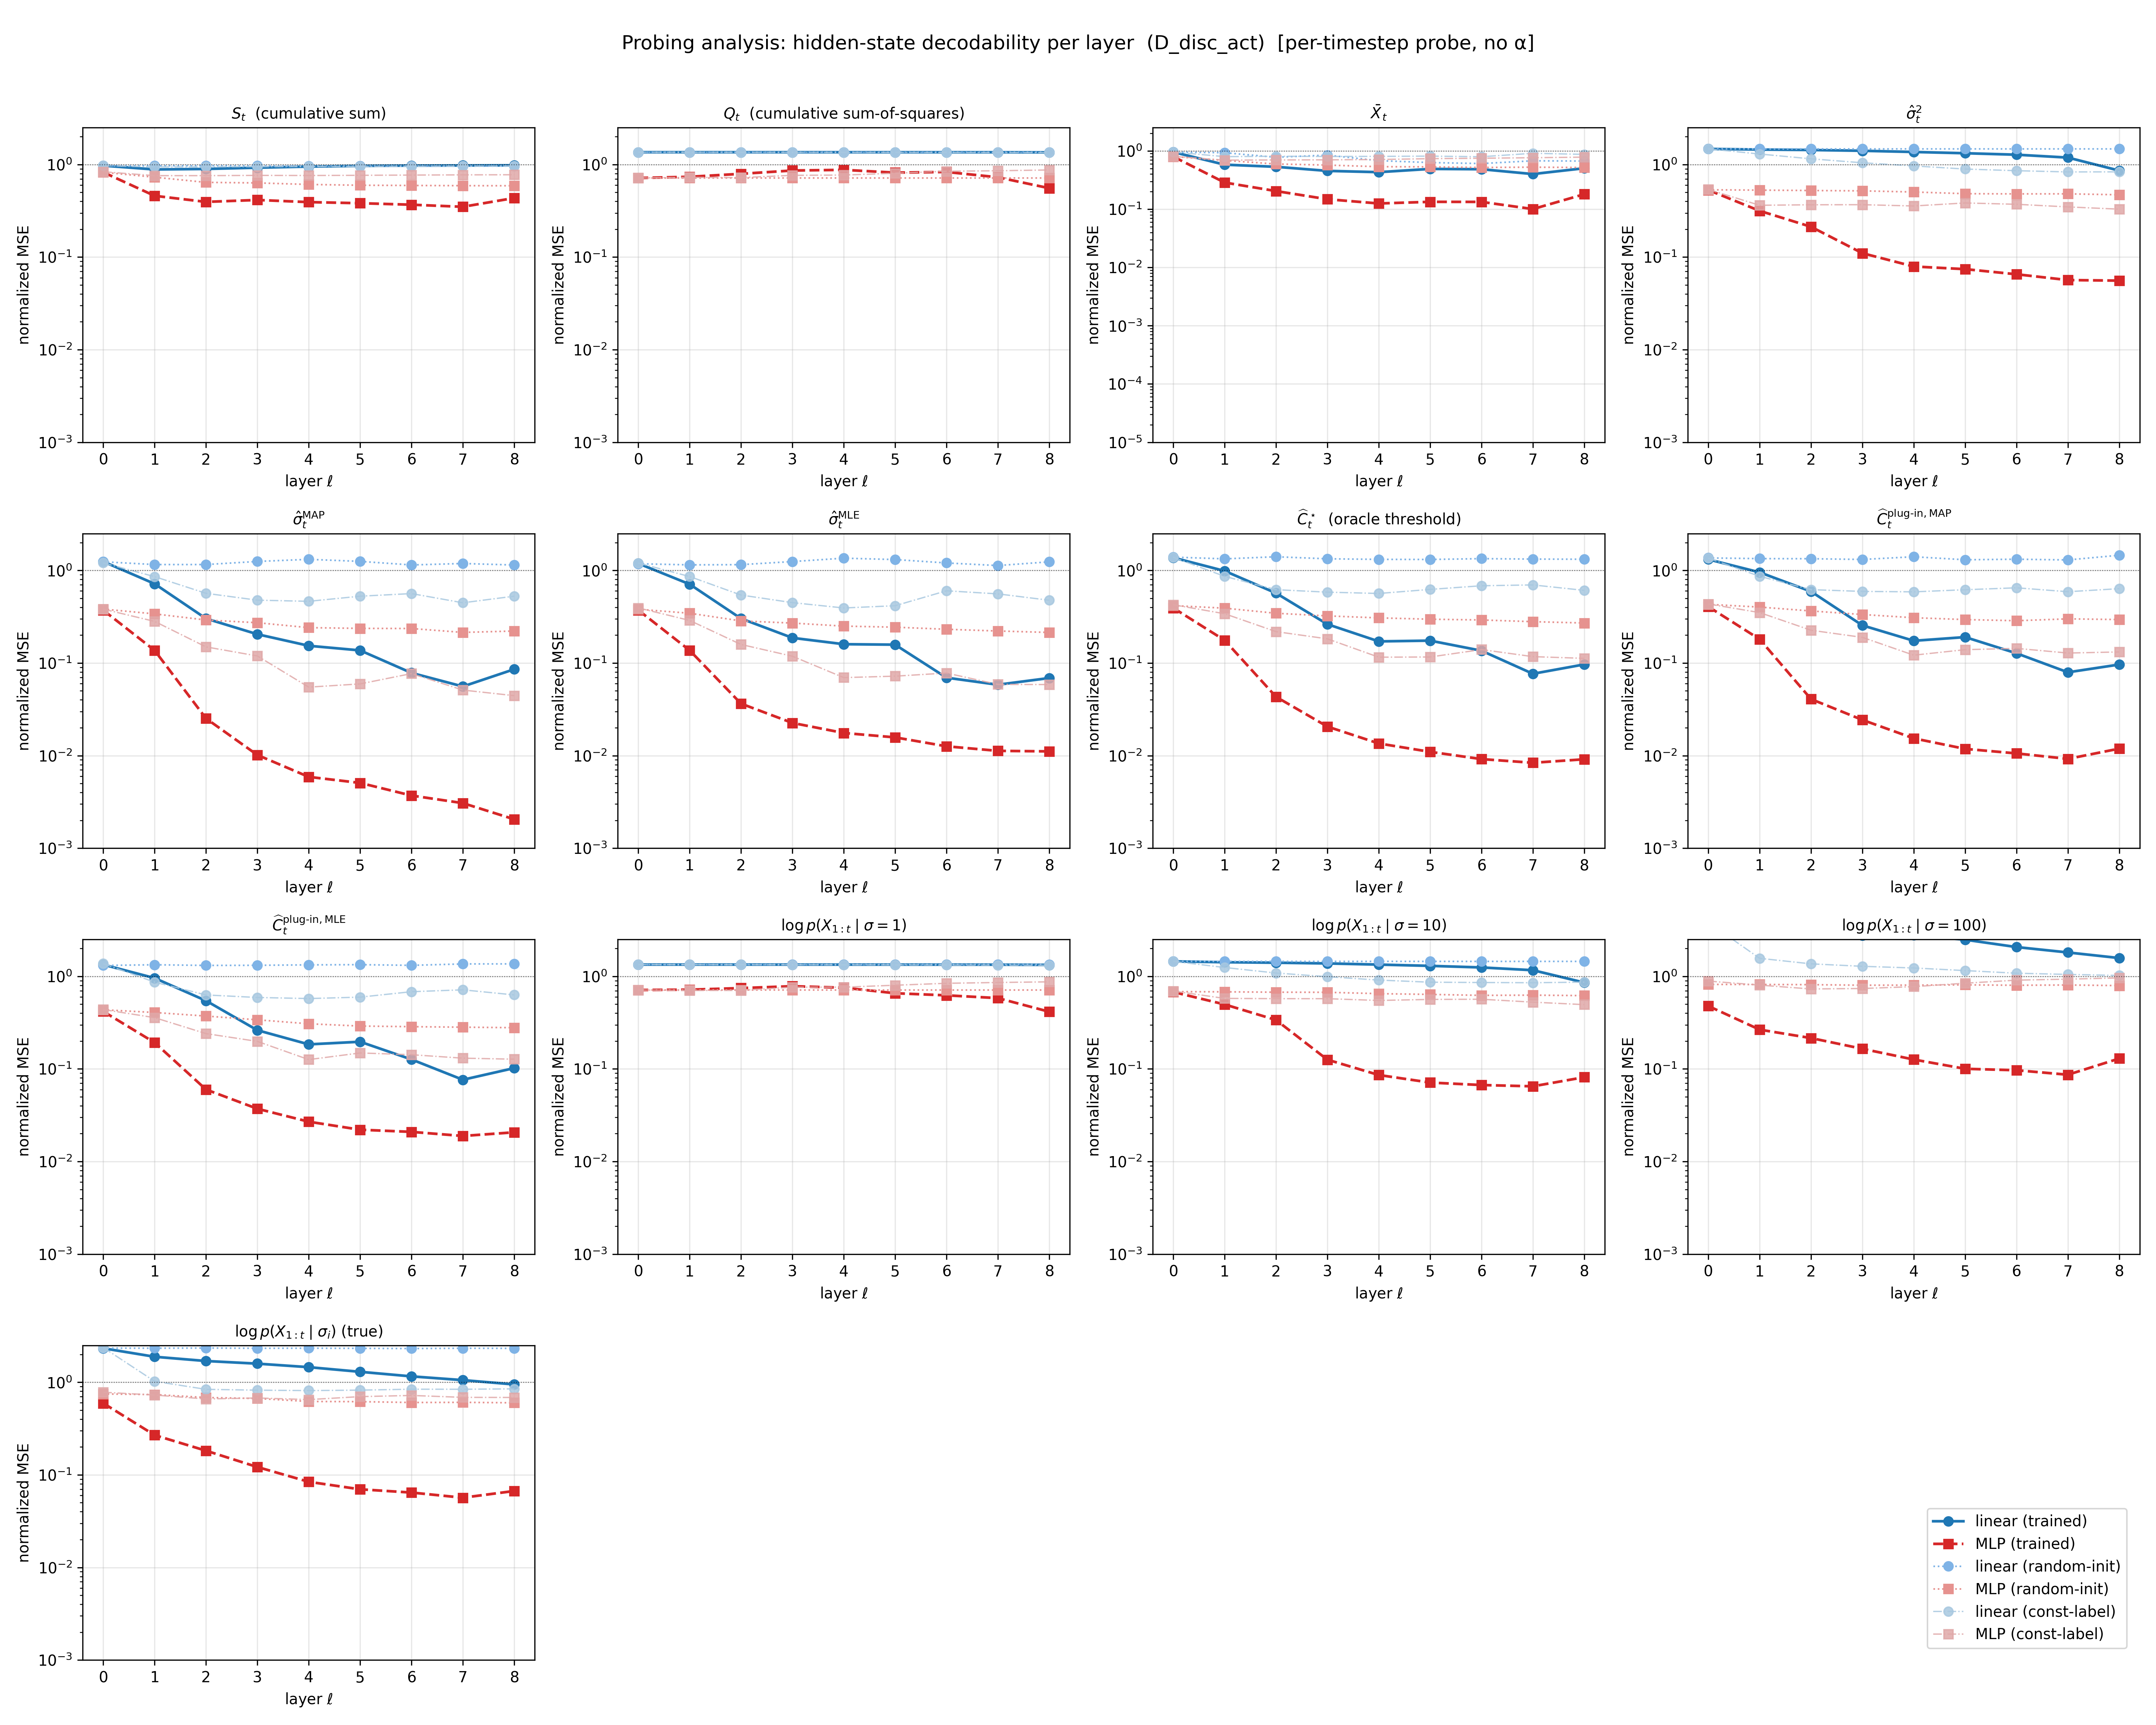
\includegraphics[width=\textwidth]{figures/probe-curves-disc-act-noattn.png}
\caption{$\mathcal{D}_{\mathrm{disc}}$\_act probing. Same layout, target list, and color scheme as Figure~\ref{fig:probe-curves-logu-act}; probe data from $\mathcal{D}_{\mathrm{disc}}$.}
\label{fig:probe-curves-disc-act}
\end{figure}

\begin{figure}[H]
\centering
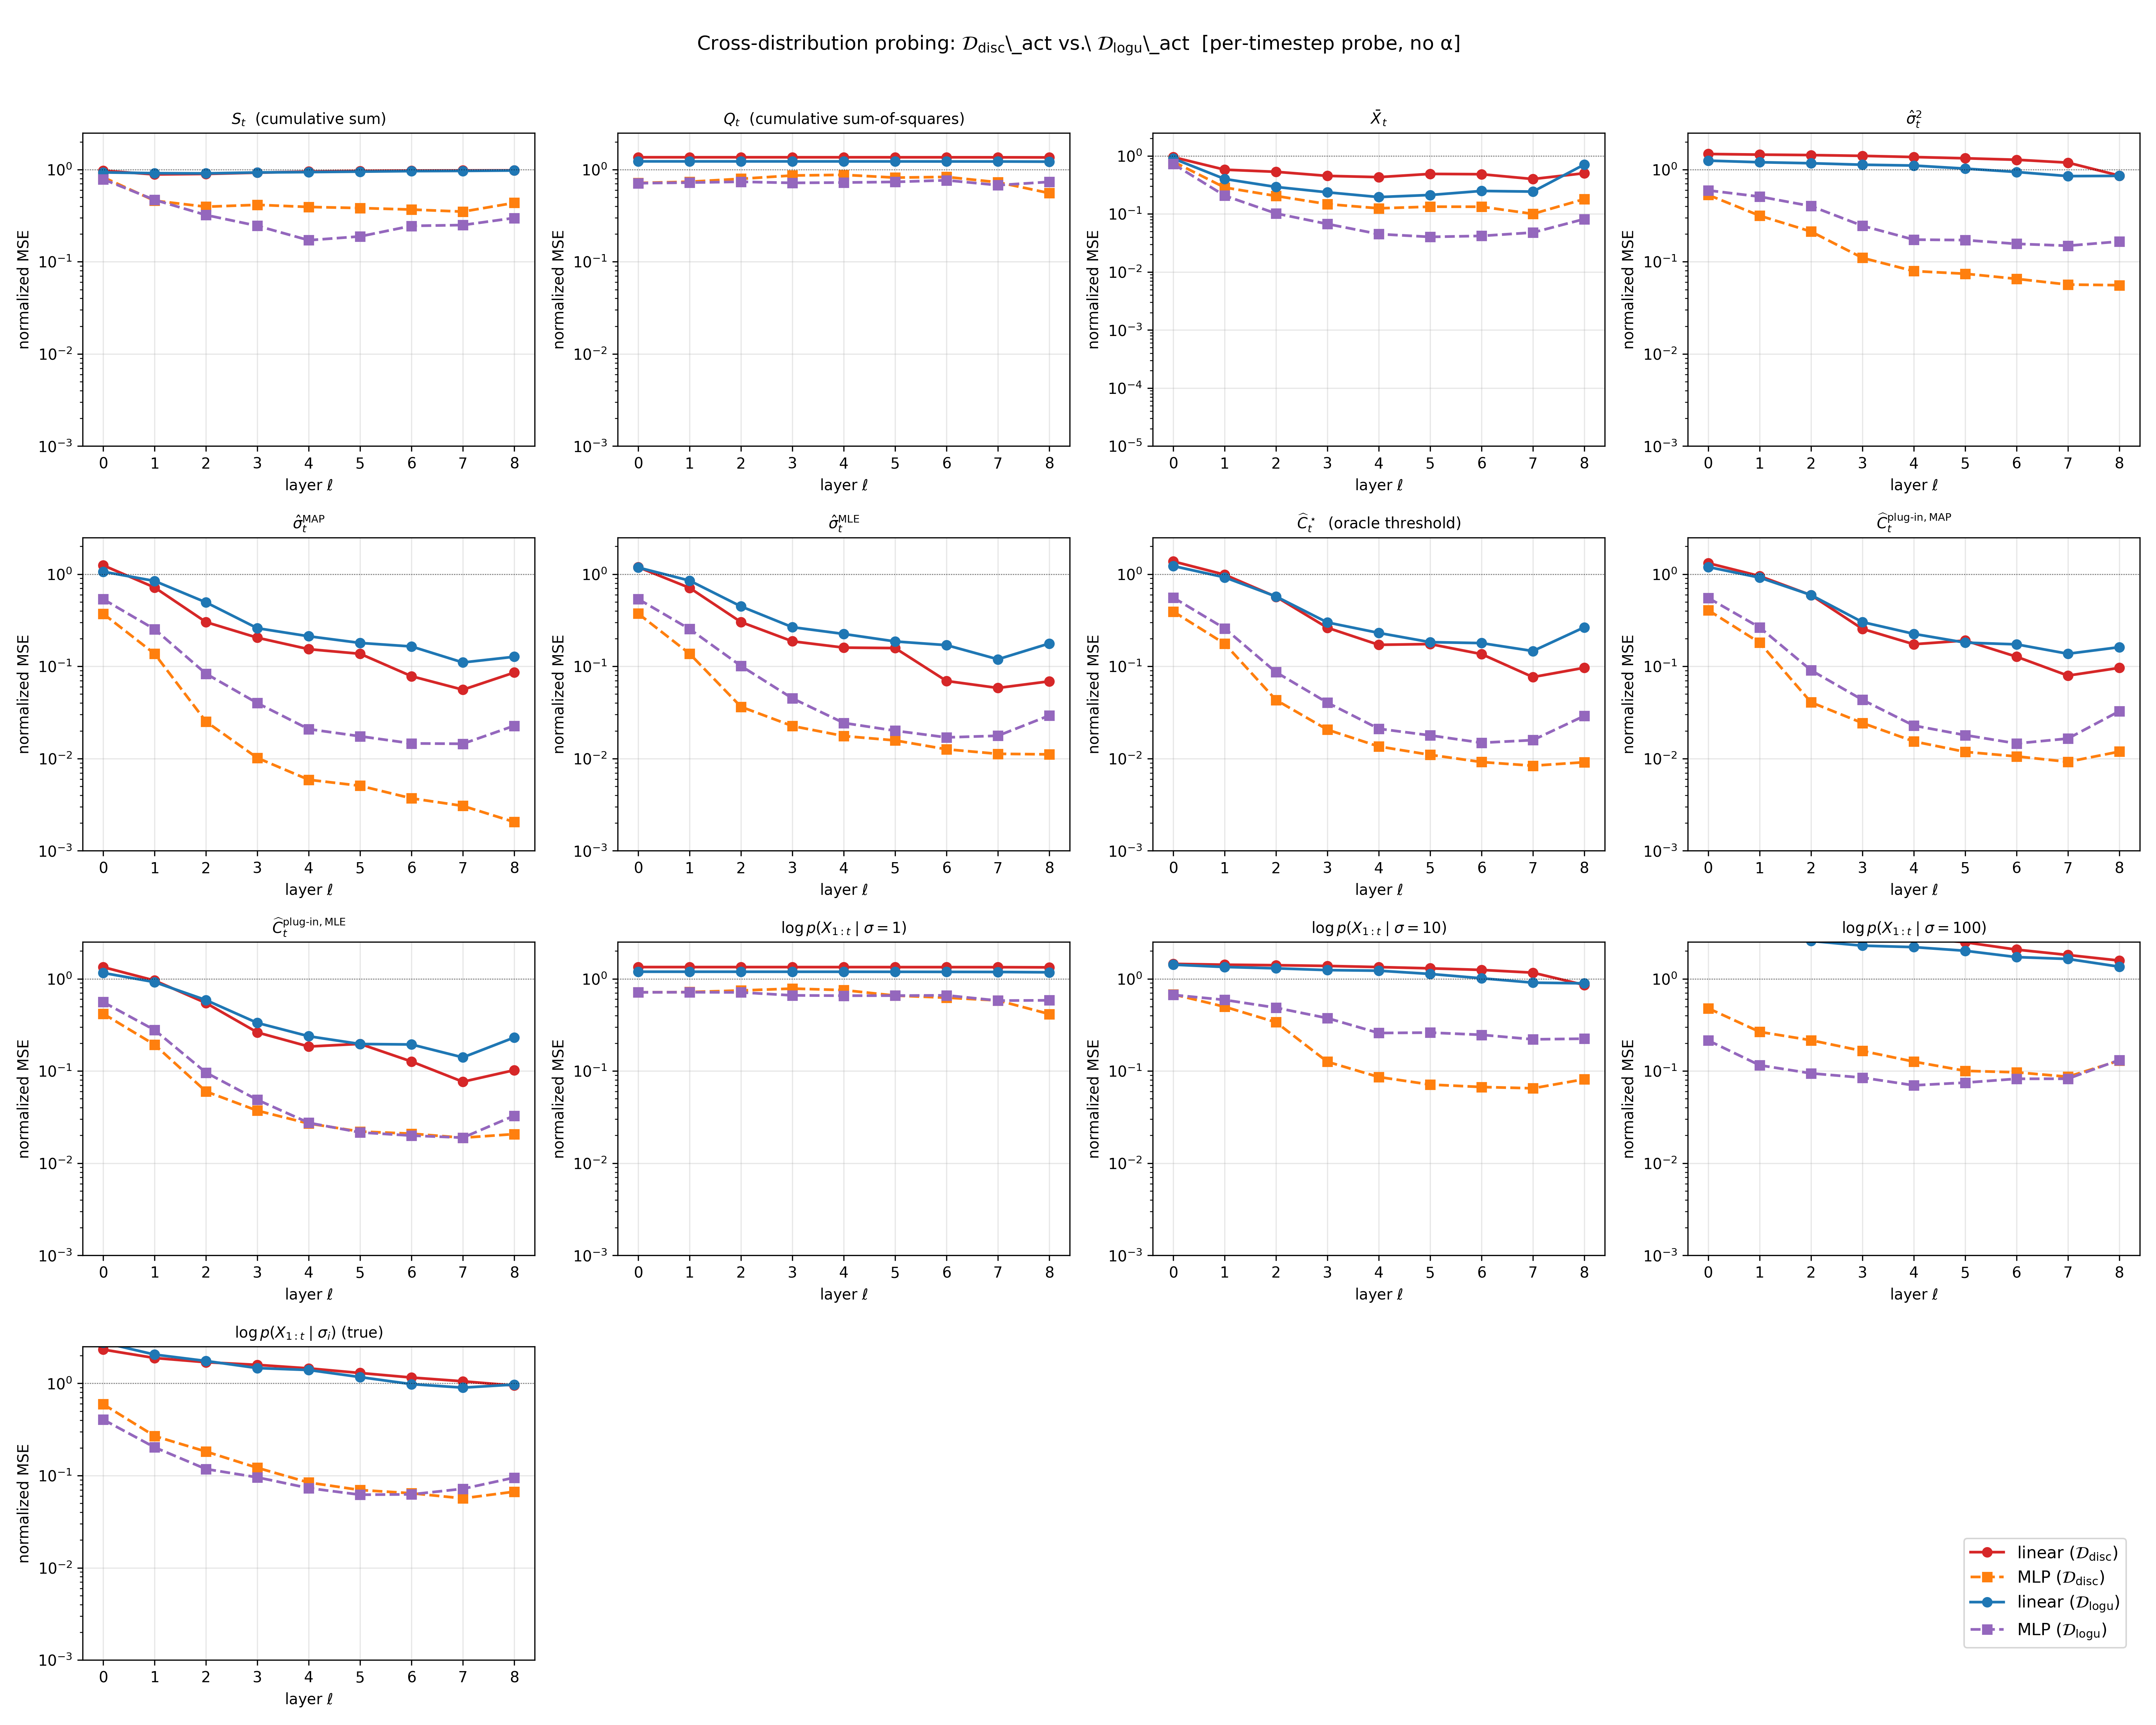
\includegraphics[width=\textwidth]{figures/probe-curves-disc-vs-logu-noattn.png}
\caption{Cross-distribution overlay, trained-probe curves only. Red / orange: $\mathcal{D}_{\mathrm{disc}}$\_act linear / MLP. Blue / purple: $\mathcal{D}_{\mathrm{logu}}$\_act linear / MLP.}
\label{fig:probe-curves-disc-vs-logu}
\end{figure}

\begin{figure}[H]
\centering
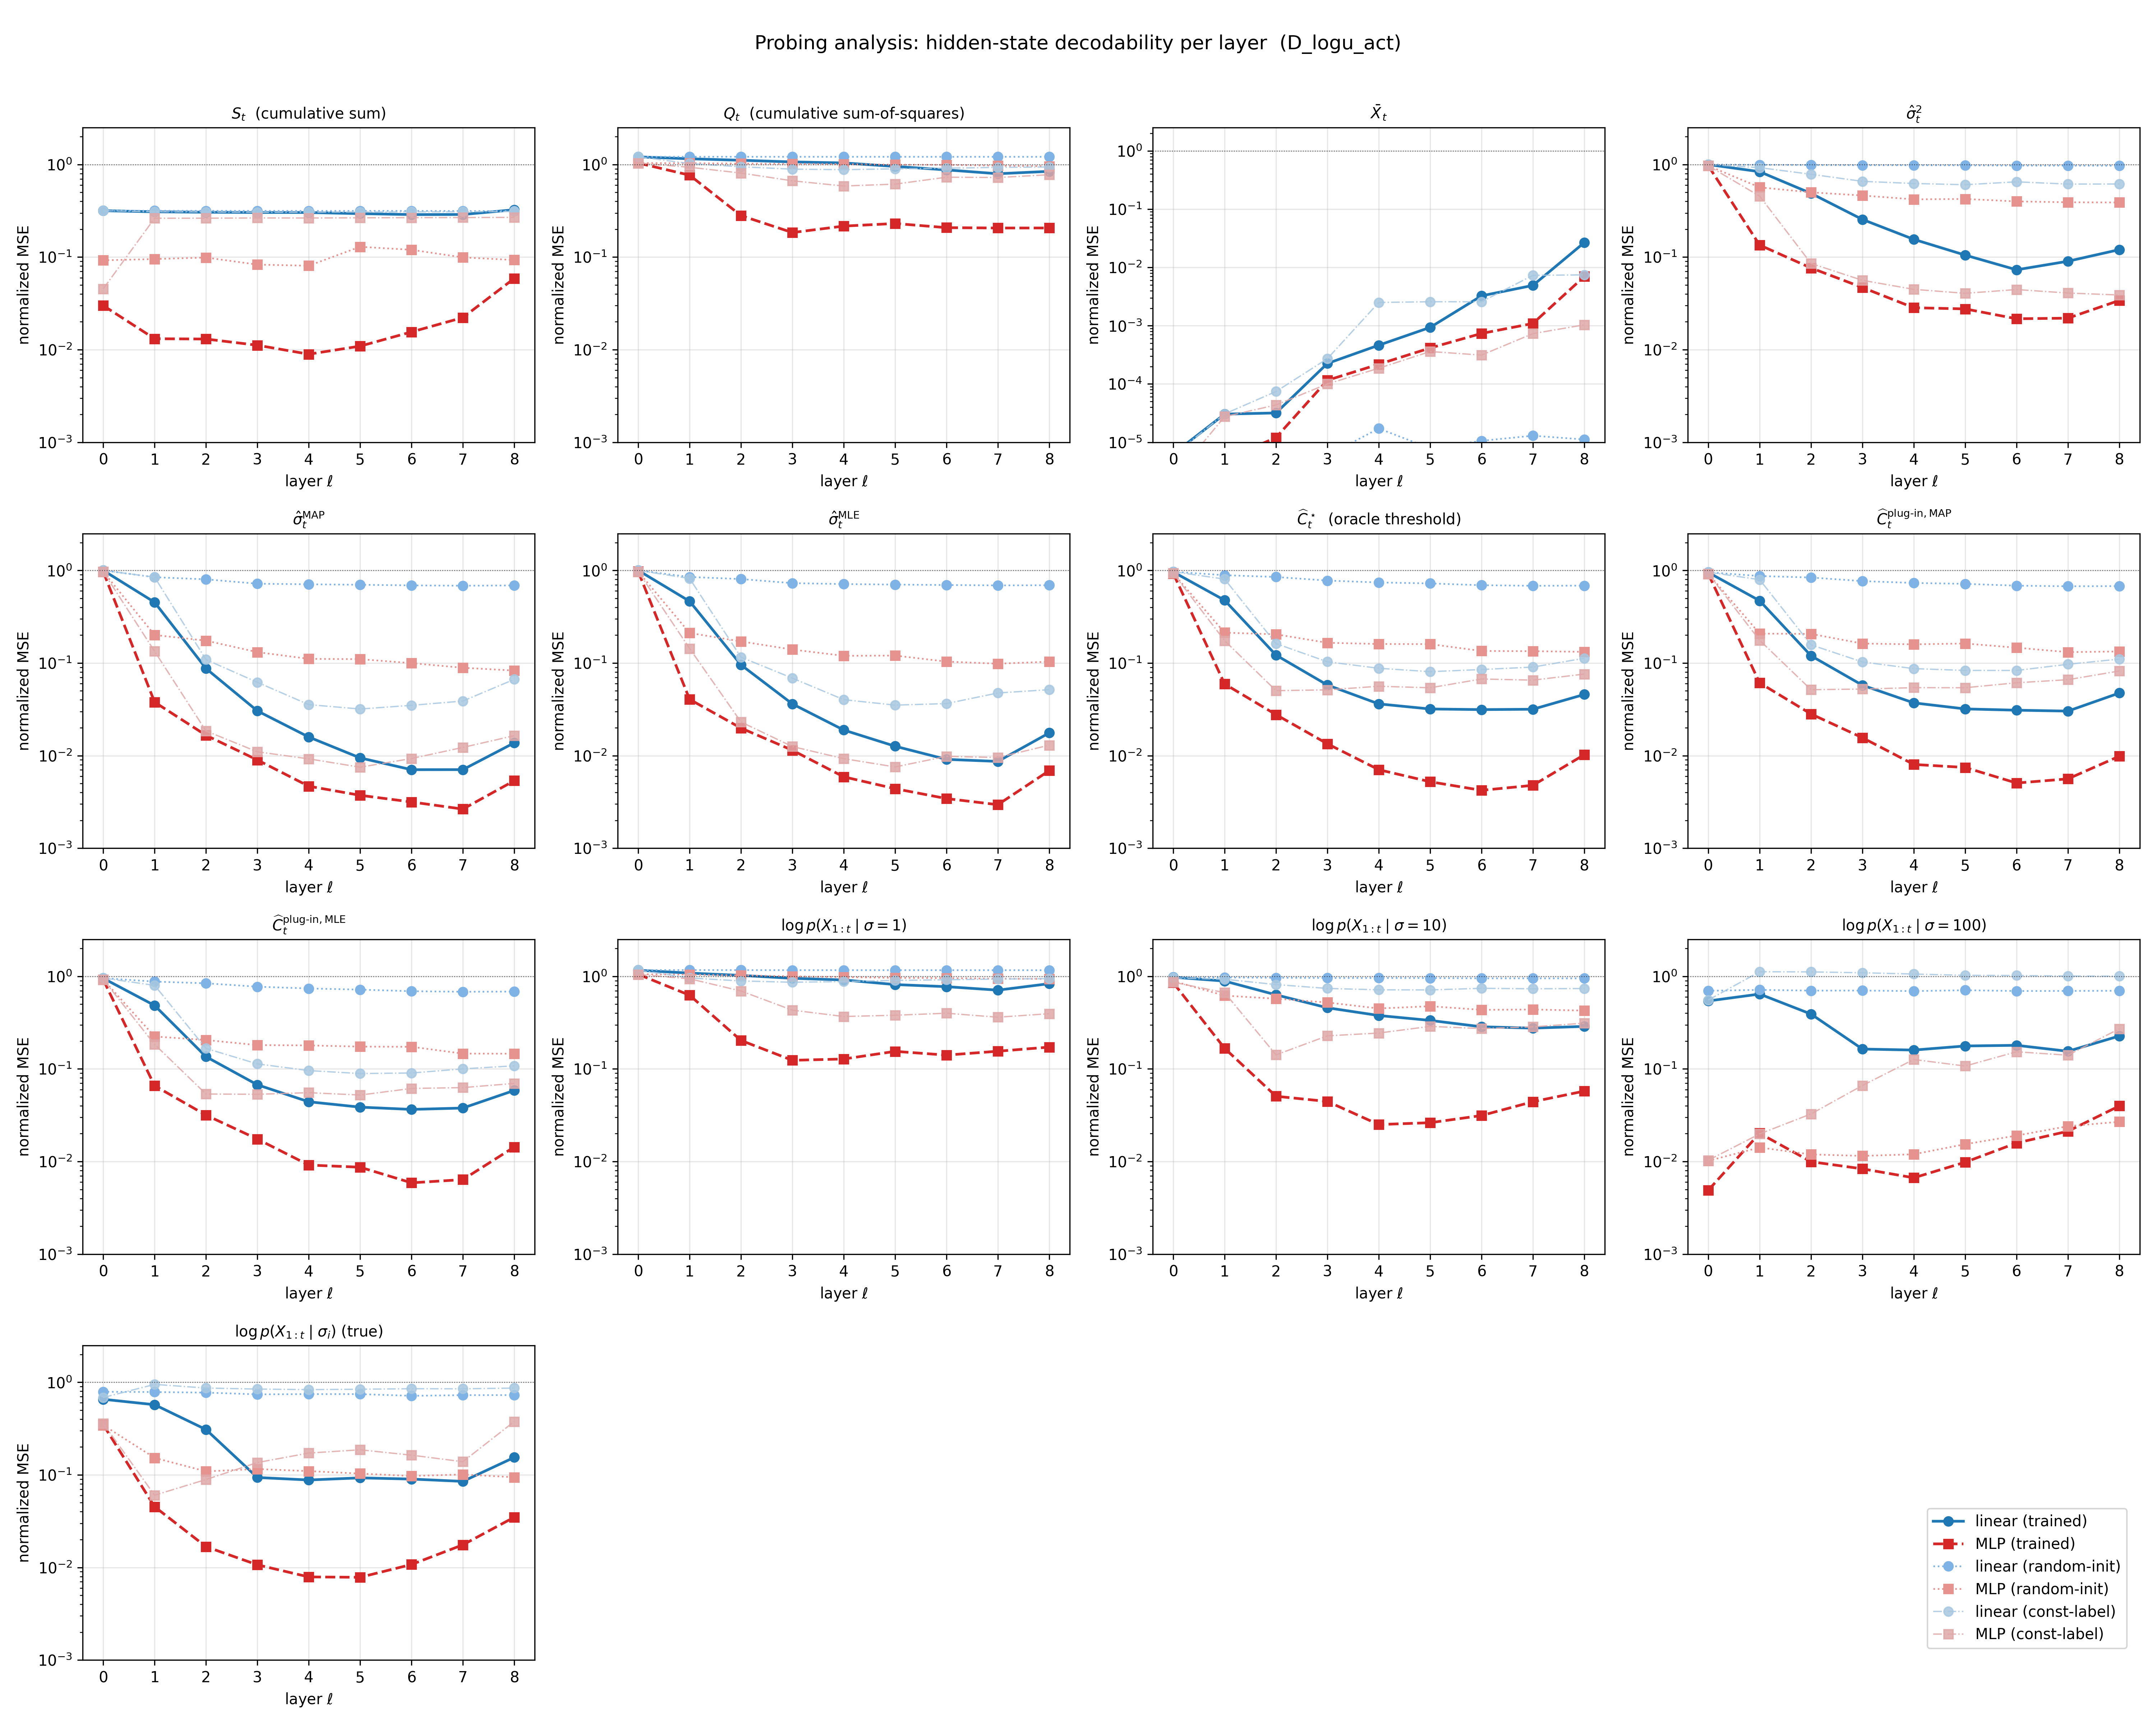
\includegraphics[width=\textwidth]{figures/probe-curves-logu-act.png}
\caption{$\mathcal{D}_{\mathrm{logu}}$\_act probing, attention-pooled probe. Same target list, layer axis, and color scheme as Figure~\ref{fig:probe-curves-logu-act}.}
\label{fig:probe-curves-logu-act-attn}
\end{figure}

\begin{figure}[H]
\centering
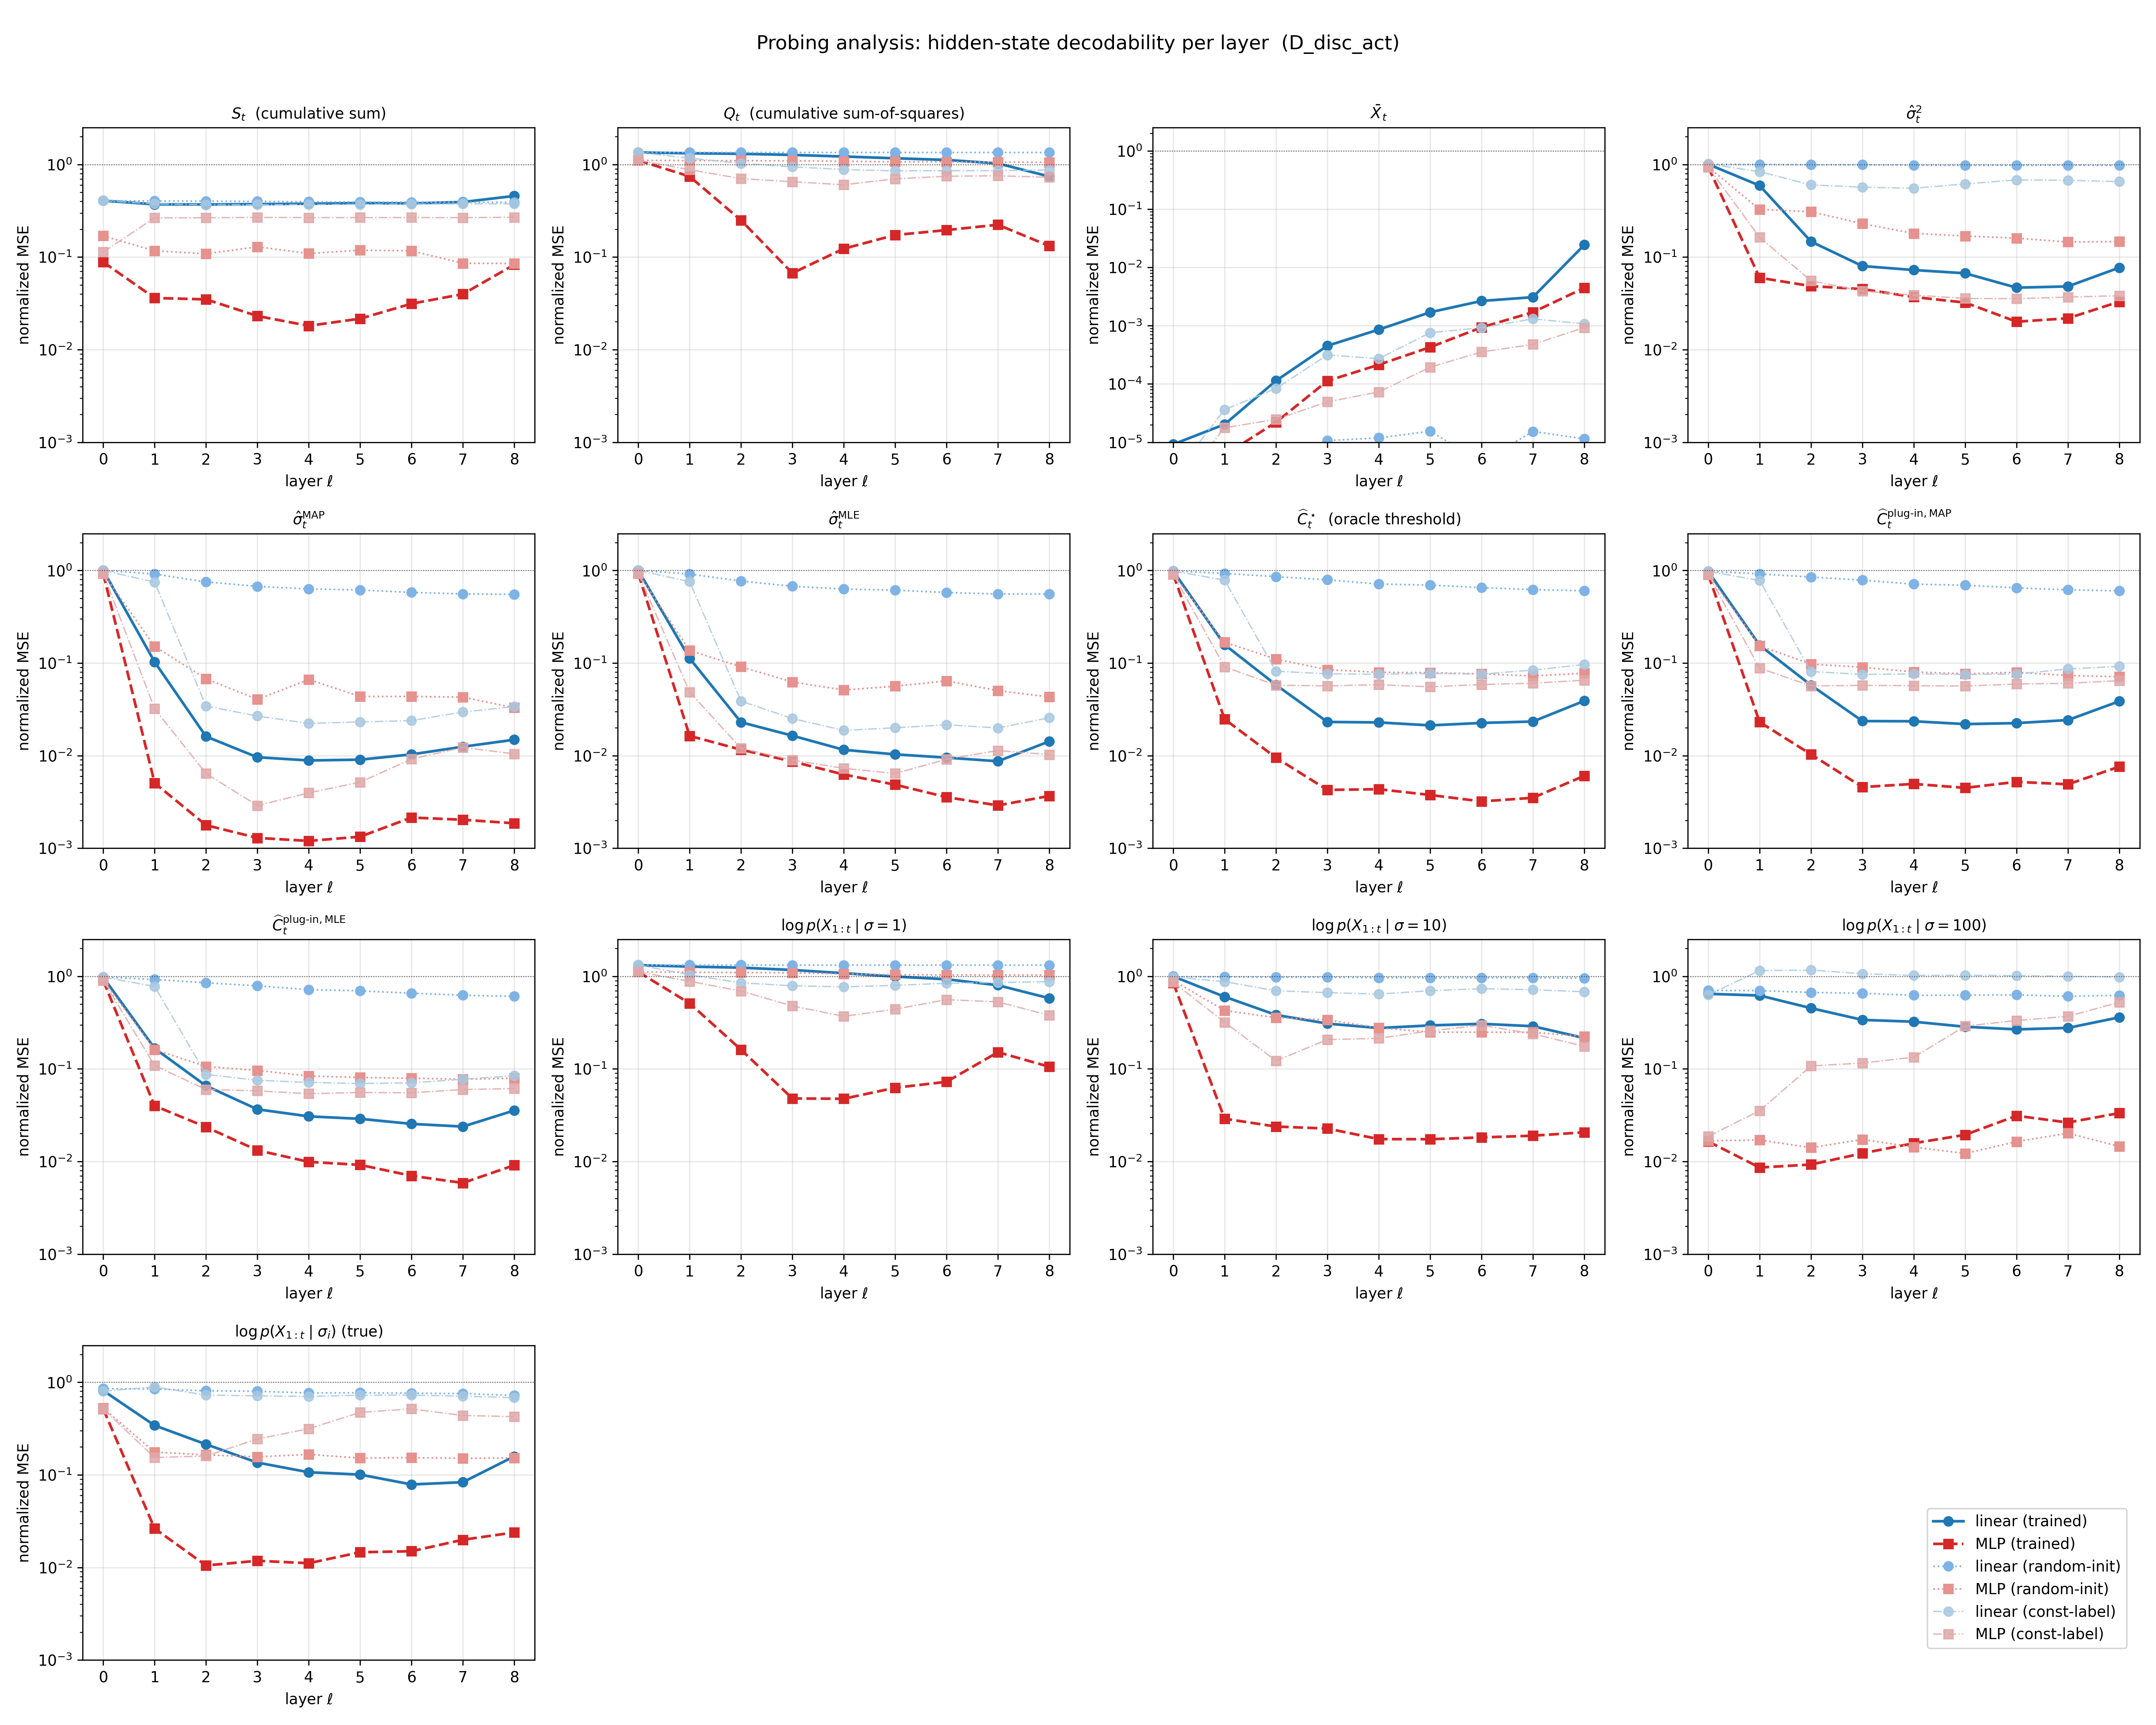
\includegraphics[width=\textwidth]{figures/probe-curves-disc-act.png}
\caption{$\mathcal{D}_{\mathrm{disc}}$\_act probing, attention-pooled probe. Same layout as Figure~\ref{fig:probe-curves-disc-act}.}
\label{fig:probe-curves-disc-act-attn}
\end{figure}

\begin{figure}[H]
\centering
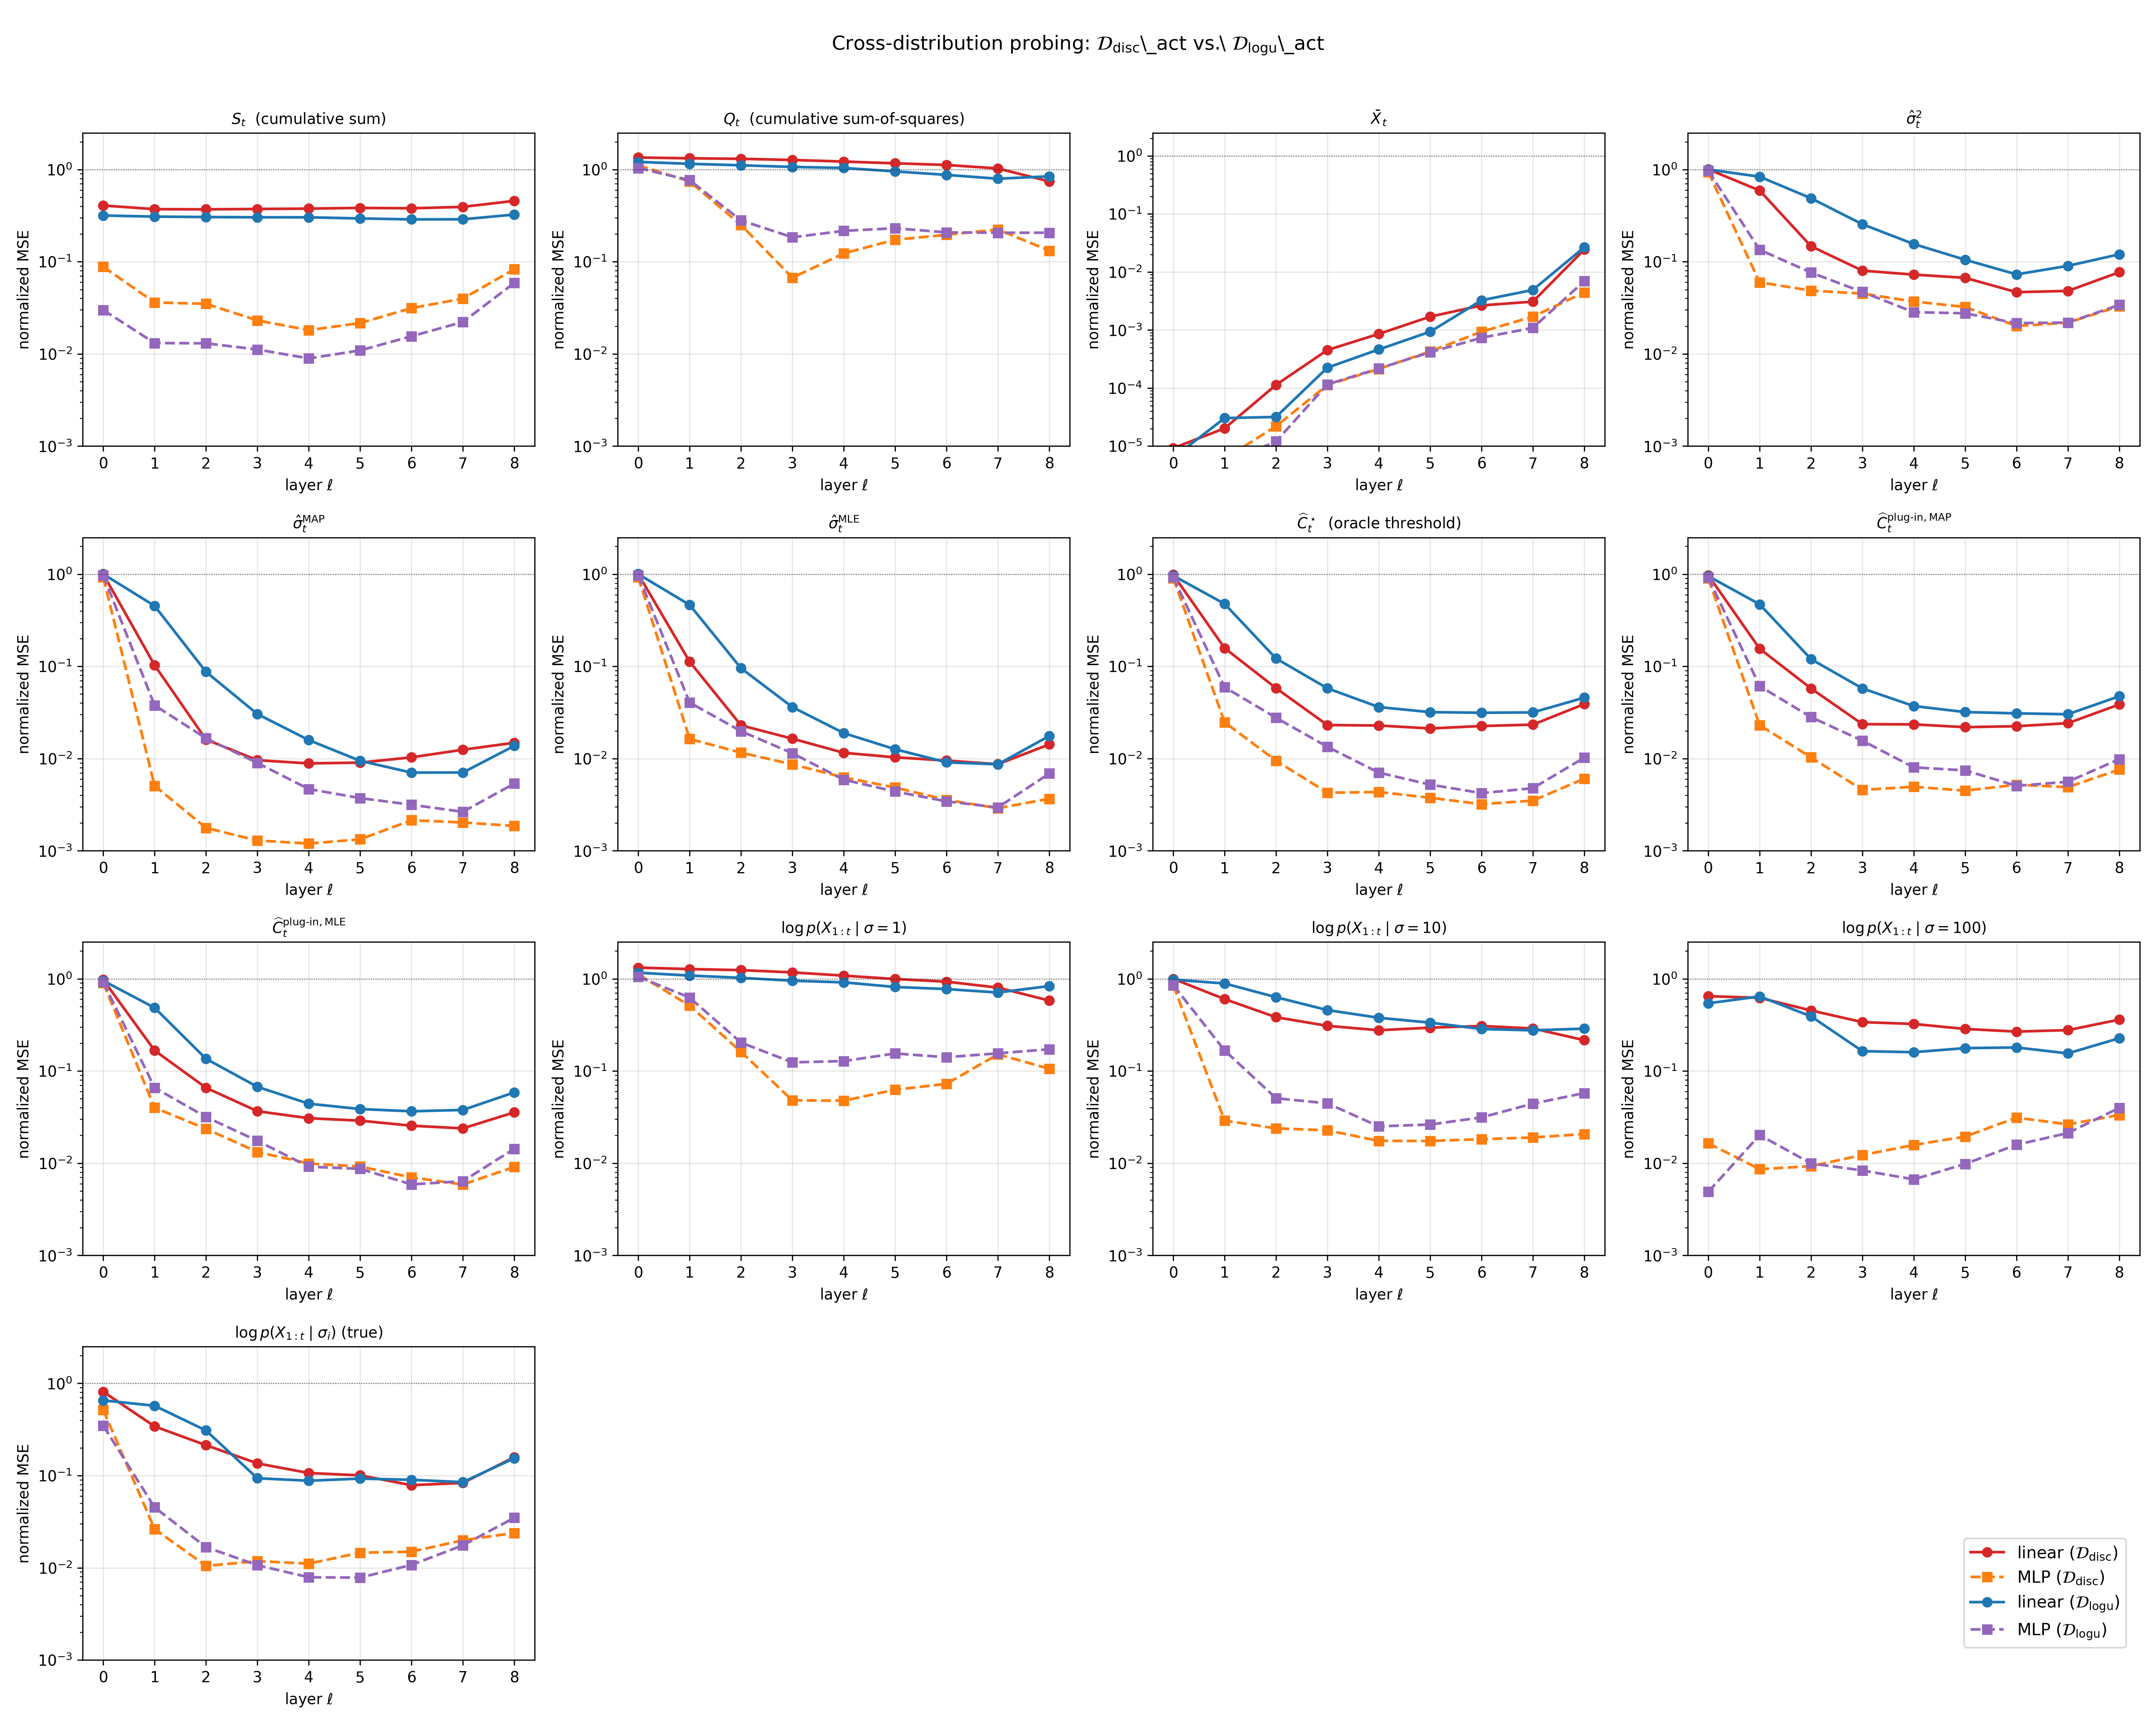
\includegraphics[width=\textwidth]{figures/probe-curves-disc-vs-logu.png}
\caption{Cross-distribution overlay, attention-pooled probe. Same color scheme as Figure~\ref{fig:probe-curves-disc-vs-logu}.}
\label{fig:probe-curves-disc-vs-logu-attn}
\end{figure}

\section{Future work}
\label{sec:future}

The remaining items of the planned mechanistic-interpretability stack are below; each tool is scoped against a specific question raised by Section~\ref{sec:results} or Section~\ref{sec:probe}.

\subsection{Attention entropy}
\label{sec:fw-attn}

The diagnostic question is whether the model develops heads that compute $\hat\sigma_t^2$. This requires multiplicative dependence on $X_s$ (squaring), distinct from the uniform-attention running-sum head needed to compute $\bar X_t$. At each position $t$, the causal attention mechanism in layer $\ell$, head $m$ produces a probability distribution $\alpha_t^{(\ell,m)} \in \Delta^{t-1}$ over the past positions $s \le t$. The number of past positions grows with $t$, so direct cross-$t$ averaging conflates structure with horizon length; we instead summarize each $\alpha_t^{(\ell,m)}$ by its normalized Shannon entropy
\[
\widetilde H_t^{(\ell, m)} \;:=\; \frac{H(\alpha_t^{(\ell, m)})}{\log(t+1)} \;\in\; [0, 1],
\]
and plot $\widetilde H_t^{(\ell, m)}$ averaged over the $N_{\mathrm{test}}$ test sequences as a function of $t$. The normalization makes the score horizon-invariant: a uniform head has $\widetilde H_t \approx 1$ at every $t$, a head concentrating on a single past position has $\widetilde H_t \approx 0$. A flat curve at $\widetilde H_t \approx 1$ identifies a candidate running-mean head; structured or low-entropy curves identify candidates for non-trivial computation. Whether such a head computes $\hat\sigma_t^2$ is then tested by the probing analysis of Section~\ref{sec:probe}.

\subsection{Causal interventions}
\label{sec:fw-intervention}

Probing is correlational: a probe direction does not establish that the model \emph{uses} the encoded quantity to set its threshold. We test causal use via vector arithmetic on the hidden states.

For a target $v$ (e.g., $\hat\sigma_t^2$ or $\hat\sigma_t^{\mathrm{MAP}}$) with linear probe direction $\mathbf{w}$ at layer $\ell$, modify the hidden state $\mathbf{h}_t^{(\ell')}$ during the forward pass at every layer $\ell' \in \{\ell, \ldots, L\}$:
\[
\mathbf{h}_t^{(\ell')} \;\leftarrow\; \mathbf{h}_t^{(\ell')} + \alpha\, \mathbf{w}.
\]
Applying at multiple layers (rather than just $\ell$) is necessary because subsequent layers can otherwise undo the intervention. Choose the scale $\alpha^\star$ so that pushing along $\mathbf{w}$ moves the probe readout from the typical $\hat\sigma_t^2$ at $\sigma = 10$ to its typical value at $\sigma = 100$.

\paragraph{Relative-shift readout.} For each random-variance model, compute three threshold trajectories averaged over the test set: $\widehat C_t^{\sigma = 10}$ on $\mathcal{D}_2$ sequences (no intervention), $\widehat C_t^{\mathrm{push}}$ on the same $\mathcal{D}_2$ sequences with $\alpha = \alpha^\star$, and $\widehat C_t^{\sigma = 100}$ on $\mathcal{D}_3$ sequences (no intervention). Plot all three, and report the relative shift
\[
\rho_t \;:=\; \frac{\widehat C_t^{\mathrm{push}} - \widehat C_t^{\sigma = 10}}{\widehat C_t^{\sigma = 100} - \widehat C_t^{\sigma = 10}}.
\]
$\rho_t = 0$ means the intervention had no effect; $\rho_t = 1$ means the model's threshold moved entirely from the $\sigma = 10$ regime to the $\sigma = 100$ regime, a signature of a causally-used variance estimate.

\subsection{Logit lens for the continuation value head}
\label{sec:fw-logit-lens}

The probing analysis tells us how target quantities are encoded layer-by-layer; ``the logit lens'' tells us when the model's \emph{output} is finalized. We apply the trained continuation-value head $\mathbf{w}_{\mathrm{cv}}^\top \mathbf{h} + b_{\mathrm{cv}}$ to the hidden state at every intermediate layer, not just the last:
\[
\widehat C_t^{(\ell)} \;:=\; \mathbf{w}_{\mathrm{cv}}^\top \mathbf{h}_t^{(\ell)} + b_{\mathrm{cv}}, \qquad \ell = 0, 1, \ldots, L.
\]
The trajectory $\ell \mapsto \widehat C_t^{(\ell)}$ shows how the predicted threshold evolves through depth. For act-supervised models we apply the act head analogously to recover $\hat a_t^{(\ell)}$.

\paragraph{Depth-of-commitment readout.} Per (model, test regime), plot the per-step trajectory of $\widehat C_t^{(\ell)}$ against $\ell$, averaged over the test set. The earliest layer at which $\widehat C_t^{(\ell)}$ matches the final-layer output to within a fixed tolerance (e.g., $1\%$) localizes the depth at which the model commits to its threshold. Combined with the layerwise probe-MSE curves of Section~\ref{sec:probe}, this orders the depths at which sufficient statistics, posterior estimates of $\sigma$, and the threshold itself become decodable.

\subsection{Activation patching}
\label{sec:fw-patching}

The hidden-state interventions of Section~\ref{sec:fw-intervention} push along a probe direction; activation patching localizes the same causal claim to specific components. Run the model on a clean sequence drawn from $\mathcal{D}_2$ (true noise level $\sigma = 10$) and a corrupt sequence drawn from $\mathcal{D}_3$ (true $\sigma = 100$). For each candidate patch site --- a (layer $\ell$, position $t'$, component $c$) triple where $c \in \{\text{attention}, \text{MLP}, \text{head}\;m\}$ --- replace the clean run's activation at that site with the corresponding corrupt activation, then complete the forward pass on the clean sequence and record the resulting $\widehat C_t^{\mathrm{patch}}$.

We report the relative shift
\[
\rho_t^{\mathrm{patch}}(\ell, t', c) \;:=\; \frac{\widehat C_t^{\mathrm{patch}} - \widehat C_t^{\mathrm{clean}}}{\widehat C_t^{\mathrm{corrupt}} - \widehat C_t^{\mathrm{clean}}}
\]
averaged over the test set, on the same $[0, 1]$ scale as Section~\ref{sec:fw-intervention}. Sites with $\rho_t^{\mathrm{patch}} \approx 1$ are individually sufficient to transport the threshold from the $\sigma = 10$ regime to $\sigma = 100$. Heatmaps over $(\ell, t')$ for each component class identify the heads or MLPs that carry the noise-level signal --- a sharper localization than the hidden-state pushing of Section~\ref{sec:fw-intervention}, which acts on all components at once.

\subsection{Head ablation at inference time}
\label{sec:fw-ablation}

Probing tells us what is encoded; ablation tells us what is used. Take a trained random-variance model and, at inference time on a held-out test set, zero or mean-replace the output of one attention head $(\ell, m)$ at all positions, leaving every other head untouched. Measure the resulting $R/R^\star$ on each test regime, and report the per-head, per-regime performance drop $\Delta_{\ell,m}^{(i)} := R/R^\star\big|_{\text{full}} - R/R^\star\big|_{\text{ablate}(\ell, m)}$ on $\mathcal{D}_i$.

The diagnostic is not just \emph{which heads are necessary} but \emph{for which regime}. A head whose ablation drops performance uniformly across $\mathcal{D}_1, \mathcal{D}_2, \mathcal{D}_3$ is doing regime-invariant work (e.g., computing $\bar X_t$). A head whose ablation drops performance only on $\mathcal{D}_3$, or whose drop scales with $\sigma$, is specifically a noise-level-handling head --- evidence that the model has learned regime-specialized circuitry. Because this requires no retraining, it can be run cheaply across all $L \times M = 32$ heads.

\end{document}
